\documentclass[twoside]{book}

% Packages required by doxygen
\usepackage{fixltx2e}
\usepackage{calc}
\usepackage{doxygen}
\usepackage[export]{adjustbox} % also loads graphicx
\usepackage{graphicx}
\usepackage[utf8]{inputenc}
\usepackage{makeidx}
\usepackage{multicol}
\usepackage{multirow}
\PassOptionsToPackage{warn}{textcomp}
\usepackage{textcomp}
\usepackage[nointegrals]{wasysym}
\usepackage[table]{xcolor}

% Font selection
\usepackage[T1]{fontenc}
\usepackage[scaled=.90]{helvet}
\usepackage{courier}
\usepackage{amssymb}
\usepackage{sectsty}
\renewcommand{\familydefault}{\sfdefault}
\allsectionsfont{%
  \fontseries{bc}\selectfont%
  \color{darkgray}%
}
\renewcommand{\DoxyLabelFont}{%
  \fontseries{bc}\selectfont%
  \color{darkgray}%
}
\newcommand{\+}{\discretionary{\mbox{\scriptsize$\hookleftarrow$}}{}{}}

% Page & text layout
\usepackage{geometry}
\geometry{%
  a4paper,%
  top=2.5cm,%
  bottom=2.5cm,%
  left=2.5cm,%
  right=2.5cm%
}
\tolerance=750
\hfuzz=15pt
\hbadness=750
\setlength{\emergencystretch}{15pt}
\setlength{\parindent}{0cm}
\setlength{\parskip}{3ex plus 2ex minus 2ex}
\makeatletter
\renewcommand{\paragraph}{%
  \@startsection{paragraph}{4}{0ex}{-1.0ex}{1.0ex}{%
    \normalfont\normalsize\bfseries\SS@parafont%
  }%
}
\renewcommand{\subparagraph}{%
  \@startsection{subparagraph}{5}{0ex}{-1.0ex}{1.0ex}{%
    \normalfont\normalsize\bfseries\SS@subparafont%
  }%
}
\makeatother

% Headers & footers
\usepackage{fancyhdr}
\pagestyle{fancyplain}
\fancyhead[LE]{\fancyplain{}{\bfseries\thepage}}
\fancyhead[CE]{\fancyplain{}{}}
\fancyhead[RE]{\fancyplain{}{\bfseries\leftmark}}
\fancyhead[LO]{\fancyplain{}{\bfseries\rightmark}}
\fancyhead[CO]{\fancyplain{}{}}
\fancyhead[RO]{\fancyplain{}{\bfseries\thepage}}
\fancyfoot[LE]{\fancyplain{}{}}
\fancyfoot[CE]{\fancyplain{}{}}
\fancyfoot[RE]{\fancyplain{}{\bfseries\scriptsize Generated by Doxygen }}
\fancyfoot[LO]{\fancyplain{}{\bfseries\scriptsize Generated by Doxygen }}
\fancyfoot[CO]{\fancyplain{}{}}
\fancyfoot[RO]{\fancyplain{}{}}
\renewcommand{\footrulewidth}{0.4pt}
\renewcommand{\chaptermark}[1]{%
  \markboth{#1}{}%
}
\renewcommand{\sectionmark}[1]{%
  \markright{\thesection\ #1}%
}

% Indices & bibliography
\usepackage{natbib}
\usepackage[titles]{tocloft}
\setcounter{tocdepth}{3}
\setcounter{secnumdepth}{5}
\makeindex

% Hyperlinks (required, but should be loaded last)
\usepackage{ifpdf}
\ifpdf
  \usepackage[pdftex,pagebackref=true]{hyperref}
\else
  \usepackage[ps2pdf,pagebackref=true]{hyperref}
\fi
\hypersetup{%
  colorlinks=true,%
  linkcolor=blue,%
  citecolor=blue,%
  unicode%
}

% Custom commands
\newcommand{\clearemptydoublepage}{%
  \newpage{\pagestyle{empty}\cleardoublepage}%
}

\usepackage{caption}
\captionsetup{labelsep=space,justification=centering,font={bf},singlelinecheck=off,skip=4pt,position=top}

%===== C O N T E N T S =====

\begin{document}

% Titlepage & ToC
\hypersetup{pageanchor=false,
             bookmarksnumbered=true,
             pdfencoding=unicode
            }
\pagenumbering{roman}
\begin{titlepage}
\vspace*{7cm}
\begin{center}%
{\Large Base\+End\+Point }\\
\vspace*{1cm}
{\large Generated by Doxygen 1.8.11}\\
\end{center}
\end{titlepage}
\clearemptydoublepage
\tableofcontents
\clearemptydoublepage
\pagenumbering{arabic}
\hypersetup{pageanchor=true}

%--- Begin generated contents ---
\chapter{Namespace Index}
\section{Namespace List}
Here is a list of all namespaces with brief descriptions\+:\begin{DoxyCompactList}
\item\contentsline{section}{\hyperlink{namespaceipc}{ipc} }{\pageref{namespaceipc}}{}
\item\contentsline{section}{\hyperlink{namespaceutils}{utils} }{\pageref{namespaceutils}}{}
\end{DoxyCompactList}

\chapter{Hierarchical Index}
\section{Class Hierarchy}
This inheritance list is sorted roughly, but not completely, alphabetically\+:\begin{DoxyCompactList}
\item \contentsline{section}{Configuration\+Data}{\pageref{classConfigurationData}}{}
\item \contentsline{section}{Configuration\+Data\+From\+Database}{\pageref{classConfigurationDataFromDatabase}}{}
\item \contentsline{section}{Database\+Details}{\pageref{classDatabaseDetails}}{}
\item \contentsline{section}{Dynamic\+Config\+Item\+Data\+Struct}{\pageref{structDynamicConfigItemDataStruct}}{}
\item \contentsline{section}{ipc\+:\+:emp\+\_\+message\+\_\+part\+\_\+after\+\_\+length}{\pageref{structipc_1_1emp__message__part__after__length}}{}
\item \contentsline{section}{ipc\+:\+:emp\+\_\+message\+\_\+part\+\_\+before\+\_\+length}{\pageref{structipc_1_1emp__message__part__before__length}}{}
\item \contentsline{section}{Encrypt\+Decrypt}{\pageref{classEncryptDecrypt}}{}
\item \contentsline{section}{ipc\+:\+:End\+Point}{\pageref{classipc_1_1EndPoint}}{}
\begin{DoxyCompactList}
\item \contentsline{section}{ipc\+:\+:Fifo}{\pageref{classipc_1_1Fifo}}{}
\item \contentsline{section}{ipc\+:\+:Pipe}{\pageref{classipc_1_1Pipe}}{}
\end{DoxyCompactList}
\item \contentsline{section}{ipc\+:\+:End\+Point\+Factory}{\pageref{classipc_1_1EndPointFactory}}{}
\item \contentsline{section}{File\+Based\+Configuration}{\pageref{classFileBasedConfiguration}}{}
\item \contentsline{section}{utils\+:\+:Log}{\pageref{classutils_1_1Log}}{}
\item \contentsline{section}{Login\+Agent}{\pageref{classLoginAgent}}{}
\item \contentsline{section}{ipc\+:\+:Socket\+End\+Point}{\pageref{classipc_1_1SocketEndPoint}}{}
\begin{DoxyCompactList}
\item \contentsline{section}{ipc\+:\+:Unix\+Domain\+Socket}{\pageref{classipc_1_1UnixDomainSocket}}{}
\end{DoxyCompactList}
\end{DoxyCompactList}

\chapter{Class Index}
\section{Class List}
Here are the classes, structs, unions and interfaces with brief descriptions\+:\begin{DoxyCompactList}
\item\contentsline{section}{\hyperlink{classConfigurationData}{Configuration\+Data} }{\pageref{classConfigurationData}}{}
\item\contentsline{section}{\hyperlink{classConfigurationDataFromDatabase}{Configuration\+Data\+From\+Database} }{\pageref{classConfigurationDataFromDatabase}}{}
\item\contentsline{section}{\hyperlink{classDatabaseDetails}{Database\+Details} }{\pageref{classDatabaseDetails}}{}
\item\contentsline{section}{\hyperlink{structDynamicConfigItemDataStruct}{Dynamic\+Config\+Item\+Data\+Struct} }{\pageref{structDynamicConfigItemDataStruct}}{}
\item\contentsline{section}{\hyperlink{structipc_1_1emp__message__part__after__length}{ipc\+::emp\+\_\+message\+\_\+part\+\_\+after\+\_\+length} }{\pageref{structipc_1_1emp__message__part__after__length}}{}
\item\contentsline{section}{\hyperlink{structipc_1_1emp__message__part__before__length}{ipc\+::emp\+\_\+message\+\_\+part\+\_\+before\+\_\+length} }{\pageref{structipc_1_1emp__message__part__before__length}}{}
\item\contentsline{section}{\hyperlink{classEncryptDecrypt}{Encrypt\+Decrypt} }{\pageref{classEncryptDecrypt}}{}
\item\contentsline{section}{\hyperlink{classipc_1_1EndPoint}{ipc\+::\+End\+Point} }{\pageref{classipc_1_1EndPoint}}{}
\item\contentsline{section}{\hyperlink{classipc_1_1EndPointFactory}{ipc\+::\+End\+Point\+Factory} }{\pageref{classipc_1_1EndPointFactory}}{}
\item\contentsline{section}{\hyperlink{classipc_1_1Fifo}{ipc\+::\+Fifo} }{\pageref{classipc_1_1Fifo}}{}
\item\contentsline{section}{\hyperlink{classFileBasedConfiguration}{File\+Based\+Configuration} }{\pageref{classFileBasedConfiguration}}{}
\item\contentsline{section}{\hyperlink{classutils_1_1Log}{utils\+::\+Log} }{\pageref{classutils_1_1Log}}{}
\item\contentsline{section}{\hyperlink{classLoginAgent}{Login\+Agent} }{\pageref{classLoginAgent}}{}
\item\contentsline{section}{\hyperlink{classipc_1_1Pipe}{ipc\+::\+Pipe} }{\pageref{classipc_1_1Pipe}}{}
\item\contentsline{section}{\hyperlink{classipc_1_1SocketEndPoint}{ipc\+::\+Socket\+End\+Point} }{\pageref{classipc_1_1SocketEndPoint}}{}
\item\contentsline{section}{\hyperlink{classipc_1_1UnixDomainSocket}{ipc\+::\+Unix\+Domain\+Socket} }{\pageref{classipc_1_1UnixDomainSocket}}{}
\end{DoxyCompactList}

\chapter{File Index}
\section{File List}
Here is a list of all files with brief descriptions\+:\begin{DoxyCompactList}
\item\contentsline{section}{C\+O\+M\+M\+O\+N/\hyperlink{EndPoint_8cpp}{End\+Point.\+cpp} }{\pageref{EndPoint_8cpp}}{}
\item\contentsline{section}{C\+O\+M\+M\+O\+N/\hyperlink{EndPoint_8h}{End\+Point.\+h} }{\pageref{EndPoint_8h}}{}
\item\contentsline{section}{C\+O\+M\+M\+O\+N/\hyperlink{EndPointFactory_8cpp}{End\+Point\+Factory.\+cpp} }{\pageref{EndPointFactory_8cpp}}{}
\item\contentsline{section}{C\+O\+M\+M\+O\+N/\hyperlink{EndPointFactory_8h}{End\+Point\+Factory.\+h} }{\pageref{EndPointFactory_8h}}{}
\item\contentsline{section}{C\+O\+M\+M\+O\+N/\hyperlink{SocketEndPoint_8cpp}{Socket\+End\+Point.\+cpp} }{\pageref{SocketEndPoint_8cpp}}{}
\item\contentsline{section}{C\+O\+M\+M\+O\+N/\hyperlink{SocketEndPoint_8h}{Socket\+End\+Point.\+h} }{\pageref{SocketEndPoint_8h}}{}
\item\contentsline{section}{Debug/\+C\+O\+M\+M\+O\+N/\hyperlink{EndPoint_8d}{End\+Point.\+d} }{\pageref{EndPoint_8d}}{}
\item\contentsline{section}{Debug/\+C\+O\+M\+M\+O\+N/\hyperlink{EndPointFactory_8d}{End\+Point\+Factory.\+d} }{\pageref{EndPointFactory_8d}}{}
\item\contentsline{section}{Debug/\+C\+O\+M\+M\+O\+N/\hyperlink{MessageReader_8d}{Message\+Reader.\+d} }{\pageref{MessageReader_8d}}{}
\item\contentsline{section}{Debug/\+C\+O\+M\+M\+O\+N/\hyperlink{SocketEndPoint_8d}{Socket\+End\+Point.\+d} }{\pageref{SocketEndPoint_8d}}{}
\item\contentsline{section}{Debug/\+I\+P\+C\+\_\+\+F\+I\+F\+O/\hyperlink{Fifo_8d}{Fifo.\+d} }{\pageref{Fifo_8d}}{}
\item\contentsline{section}{Debug/\+I\+P\+C\+\_\+\+P\+I\+P\+E/\hyperlink{Pipe_8d}{Pipe.\+d} }{\pageref{Pipe_8d}}{}
\item\contentsline{section}{Debug/\+I\+P\+C\+\_\+\+U\+D\+S/\hyperlink{UnixDomainSocket_8d}{Unix\+Domain\+Socket.\+d} }{\pageref{UnixDomainSocket_8d}}{}
\item\contentsline{section}{Debug/\+L\+O\+G/\hyperlink{Log_8d}{Log.\+d} }{\pageref{Log_8d}}{}
\item\contentsline{section}{Debug/\+L\+O\+G/\hyperlink{main_8d}{main.\+d} }{\pageref{main_8d}}{}
\item\contentsline{section}{Debug/\+T\+E\+S\+T/\hyperlink{GtestMain_8d}{Gtest\+Main.\+d} }{\pageref{GtestMain_8d}}{}
\item\contentsline{section}{Debug/\+T\+E\+S\+T/\hyperlink{TestIPCTechniques_8d}{Test\+I\+P\+C\+Techniques.\+d} }{\pageref{TestIPCTechniques_8d}}{}
\item\contentsline{section}{D\+Y\+N\+\_\+\+C\+O\+N\+F\+I\+G/include/\hyperlink{ConfigurationData_8h}{Configuration\+Data.\+h} }{\pageref{ConfigurationData_8h}}{}
\item\contentsline{section}{D\+Y\+N\+\_\+\+C\+O\+N\+F\+I\+G/include/\hyperlink{ConfigurationDataFromDatabase_8h}{Configuration\+Data\+From\+Database.\+h} }{\pageref{ConfigurationDataFromDatabase_8h}}{}
\item\contentsline{section}{D\+Y\+N\+\_\+\+C\+O\+N\+F\+I\+G/include/\hyperlink{DatabaseDetails_8h}{Database\+Details.\+h} }{\pageref{DatabaseDetails_8h}}{}
\item\contentsline{section}{D\+Y\+N\+\_\+\+C\+O\+N\+F\+I\+G/include/\hyperlink{DynamicConfigItemDataStruct_8h}{Dynamic\+Config\+Item\+Data\+Struct.\+h} }{\pageref{DynamicConfigItemDataStruct_8h}}{}
\item\contentsline{section}{D\+Y\+N\+\_\+\+C\+O\+N\+F\+I\+G/include/\hyperlink{EncryptDecrypt_8h}{Encrypt\+Decrypt.\+h} }{\pageref{EncryptDecrypt_8h}}{}
\item\contentsline{section}{D\+Y\+N\+\_\+\+C\+O\+N\+F\+I\+G/include/\hyperlink{FileBasedConfiguration_8h}{File\+Based\+Configuration.\+h} }{\pageref{FileBasedConfiguration_8h}}{}
\item\contentsline{section}{D\+Y\+N\+\_\+\+C\+O\+N\+F\+I\+G/include/\hyperlink{LoginAgent_8h}{Login\+Agent.\+h} }{\pageref{LoginAgent_8h}}{}
\item\contentsline{section}{D\+Y\+N\+\_\+\+C\+O\+N\+F\+I\+G/include/\hyperlink{OraError_8h}{Ora\+Error.\+h} }{\pageref{OraError_8h}}{}
\item\contentsline{section}{I\+P\+C\+\_\+\+F\+I\+F\+O/\hyperlink{Fifo_8cpp}{Fifo.\+cpp} }{\pageref{Fifo_8cpp}}{}
\item\contentsline{section}{I\+P\+C\+\_\+\+F\+I\+F\+O/\hyperlink{Fifo_8h}{Fifo.\+h} }{\pageref{Fifo_8h}}{}
\item\contentsline{section}{I\+P\+C\+\_\+\+P\+I\+P\+E/\hyperlink{Pipe_8cpp}{Pipe.\+cpp} }{\pageref{Pipe_8cpp}}{}
\item\contentsline{section}{I\+P\+C\+\_\+\+P\+I\+P\+E/\hyperlink{Pipe_8h}{Pipe.\+h} }{\pageref{Pipe_8h}}{}
\item\contentsline{section}{I\+P\+C\+\_\+\+U\+D\+S/\hyperlink{UnixDomainSocket_8cpp}{Unix\+Domain\+Socket.\+cpp} }{\pageref{UnixDomainSocket_8cpp}}{}
\item\contentsline{section}{I\+P\+C\+\_\+\+U\+D\+S/\hyperlink{UnixDomainSocket_8h}{Unix\+Domain\+Socket.\+h} }{\pageref{UnixDomainSocket_8h}}{}
\item\contentsline{section}{L\+O\+G/\hyperlink{Log_8cpp}{Log.\+cpp} }{\pageref{Log_8cpp}}{}
\item\contentsline{section}{L\+O\+G/\hyperlink{Log_8h}{Log.\+h} }{\pageref{Log_8h}}{}
\item\contentsline{section}{L\+O\+G/\hyperlink{main_8cpp}{main.\+cpp} }{\pageref{main_8cpp}}{}
\item\contentsline{section}{T\+E\+S\+T/\hyperlink{GtestMain_8cpp}{Gtest\+Main.\+cpp} }{\pageref{GtestMain_8cpp}}{}
\item\contentsline{section}{T\+E\+S\+T/\hyperlink{TestIPCTechniques_8cpp}{Test\+I\+P\+C\+Techniques.\+cpp} }{\pageref{TestIPCTechniques_8cpp}}{}
\end{DoxyCompactList}

\chapter{Namespace Documentation}
\hypertarget{namespaceipc}{}\section{ipc Namespace Reference}
\label{namespaceipc}\index{ipc@{ipc}}
\subsection*{Classes}
\begin{DoxyCompactItemize}
\item 
struct \hyperlink{structipc_1_1emp__message__part__after__length}{emp\+\_\+message\+\_\+part\+\_\+after\+\_\+length}
\item 
struct \hyperlink{structipc_1_1emp__message__part__before__length}{emp\+\_\+message\+\_\+part\+\_\+before\+\_\+length}
\item 
class \hyperlink{classipc_1_1EndPoint}{End\+Point}
\item 
class \hyperlink{classipc_1_1EndPointFactory}{End\+Point\+Factory}
\item 
class \hyperlink{classipc_1_1Fifo}{Fifo}
\item 
class \hyperlink{classipc_1_1Pipe}{Pipe}
\item 
class \hyperlink{classipc_1_1SocketEndPoint}{Socket\+End\+Point}
\item 
class \hyperlink{classipc_1_1UnixDomainSocket}{Unix\+Domain\+Socket}
\end{DoxyCompactItemize}

\hypertarget{namespaceutils}{}\section{utils Namespace Reference}
\label{namespaceutils}\index{utils@{utils}}
\subsection*{Classes}
\begin{DoxyCompactItemize}
\item 
class \hyperlink{classutils_1_1Log}{Log}
\end{DoxyCompactItemize}

\chapter{Class Documentation}
\hypertarget{classConfigurationData}{}\section{Configuration\+Data Class Reference}
\label{classConfigurationData}\index{Configuration\+Data@{Configuration\+Data}}


{\ttfamily \#include $<$Configuration\+Data.\+h$>$}

\subsection*{Public Types}
\begin{DoxyCompactItemize}
\item 
enum \hyperlink{classConfigurationData_a6b159be92b02274088a4de34584eeabc}{Data\+Source} \{ \hyperlink{classConfigurationData_a6b159be92b02274088a4de34584eeabca9e0c7b9239487cfb4752209277ac79aa}{F\+I\+LE}, 
\hyperlink{classConfigurationData_a6b159be92b02274088a4de34584eeabca30f2137384653ca12f00f3bc62a807ea}{DB}, 
\hyperlink{classConfigurationData_a6b159be92b02274088a4de34584eeabca38caa02da39a1a3ed2b30b02f3153a8f}{E\+N\+D\+\_\+\+O\+F\+\_\+\+Data\+Source}
 \}
\item 
typedef map$<$ std\+::string, std\+::vector$<$ \hyperlink{structDynamicConfigItemDataStruct}{Dynamic\+Config\+Item\+Data\+Struct} $>$ $>$ \hyperlink{classConfigurationData_a88b45bf304a35e4e78cfce6688087cce}{configuration\+Data\+\_\+map\+\_\+t}
\end{DoxyCompactItemize}
\subsection*{Public Member Functions}
\begin{DoxyCompactItemize}
\item 
\hyperlink{classConfigurationData_a8cb8af69711def4253a59956e7b33c15}{Configuration\+Data} ()
\item 
virtual \hyperlink{classConfigurationData_a4f90f14791e6c4dc6836dffab3ae49ae}{$\sim$\+Configuration\+Data} ()
\item 
\hyperlink{ConfigurationData_8h_a4e9a8de26cf7d053d8e1db76220bdc33}{Dyn\+Cfg\+Intf\+Return\+Codes} \hyperlink{classConfigurationData_a85ef47317952a9369b474c8df2525322}{Get\+Configuration\+Data} ()
\item 
\hyperlink{ConfigurationData_8h_a4e9a8de26cf7d053d8e1db76220bdc33}{Dyn\+Cfg\+Intf\+Return\+Codes} \hyperlink{classConfigurationData_ae3be498bfc92a2162247810dfb37f6ec}{Get\+Configuration\+Data\+From\+File} (const std\+::string file\+Name, bool is\+Success)
\item 
\hyperlink{ConfigurationData_8h_a4e9a8de26cf7d053d8e1db76220bdc33}{Dyn\+Cfg\+Intf\+Return\+Codes} \hyperlink{classConfigurationData_aa5fd34a8fabbe045ec9b607a94fc021c}{Get\+Configuration\+Data\+From\+Db} (string svcname, bool is\+Success)
\item 
{\footnotesize template$<$typename T $>$ }\\T \hyperlink{classConfigurationData_a5960620b5e6e32d288157bb35860aa4d}{Get\+Configuration\+Item\+Value} (string str\+Group\+Name, string str\+Item\+Name, T t\+Def\+Item\+Value)
\item 
bool \hyperlink{classConfigurationData_a37a40d143e56aa3577cace34049091df}{get\+Group\+Name} (const std\+::string str\+Group\+\_\+c, vector$<$ \hyperlink{structDynamicConfigItemDataStruct}{Dynamic\+Config\+Item\+Data\+Struct} $>$ \&vt\+\_\+config\+Data)
\item 
bool \hyperlink{classConfigurationData_a4d298695a36f8537adff911698e8da6a}{get\+Bool\+Type\+Item\+Value} (string str\+Group\+Name, string str\+Item\+Name, bool b\+Def\+Item\+Value=false)
\item 
int \hyperlink{classConfigurationData_a54bb3e76dfb9e720bbcb41a277e1aee1}{get\+Int\+Type\+Item\+Value} (string str\+Group\+Name, string str\+Item\+Name, int n\+Def\+Item\+Value=0)
\item 
long \hyperlink{classConfigurationData_ace8acd6f1471ffc98cc2df5e526d7e3a}{get\+Long\+Type\+Item\+Value} (string str\+Group\+Name, string str\+Item\+Name, long l\+Def\+Item\+Value=0)
\item 
double \hyperlink{classConfigurationData_aa3255f642441d984e8963896a22eeb04}{get\+Double\+Type\+Item\+Value} (string str\+Group\+Name, string str\+Item\+Name, double d\+Def\+Item\+Value=0.\+0)
\item 
char \hyperlink{classConfigurationData_a81813d9b987a56d31b1d49db4f308746}{get\+Char\+Type\+Item\+Value} (string str\+Group\+Name, string str\+Item\+Name, char def\+Item\+Value= \textquotesingle{}\textbackslash{}0\textquotesingle{})
\item 
string \hyperlink{classConfigurationData_a59866f345224cbf203c835e0693771b9}{get\+String\+Type\+Item\+Value} (string str\+Group\+Name, string str\+Item\+Name, string str\+Def\+Item\+Value=\char`\"{}\char`\"{})
\item 
std\+::vector$<$ std\+::string $>$ \& \hyperlink{classConfigurationData_af68323f3fea60118d8150ad469bd2a0a}{get\+Item\+Value\+String\+List} (string str\+Group\+Name, string str\+Item\+Name)
\item 
std\+::vector$<$ std\+::pair$<$ std\+::string, std\+::string $>$ $>$ \hyperlink{classConfigurationData_acab5cb404d738f84daed25f604f692e4}{get\+Name\+Value\+List} (string str\+Group\+Name)
\item 
bool \hyperlink{classConfigurationData_a93380d92256f8798651a07fce30f7d83}{print\+Configuration\+Data} ()
\item 
bool \hyperlink{classConfigurationData_a7c04864007d1a78c1881b1ab83d78698}{get\+Item\+Name\+Found} ()
\item 
\hyperlink{classConfigurationData_a88b45bf304a35e4e78cfce6688087cce}{configuration\+Data\+\_\+map\+\_\+t} \hyperlink{classConfigurationData_a7a2e42c0440473858c382c39e3d66f3a}{get\+Configuration\+Data} ()
\item 
\hyperlink{classConfigurationData_a6b159be92b02274088a4de34584eeabc}{Data\+Source} \hyperlink{classConfigurationData_a10b79d03076c79b4e16aeed78f50a427}{Get\+Data\+Source} ()
\item 
void \hyperlink{classConfigurationData_ac5288ab51744fc8697a24d2663136916}{Set\+Data\+Source} (\hyperlink{classConfigurationData_a6b159be92b02274088a4de34584eeabc}{Data\+Source} source)
\item 
const std\+::string \& \hyperlink{classConfigurationData_abc7059c19e27c48a05ef4184c73a26bc}{Get\+File\+Name} ()
\item 
void \hyperlink{classConfigurationData_a54f43e41906262c4a336b370a4f1726c}{Set\+File\+Name} (string str\+File\+Name)
\item 
const std\+::string \& \hyperlink{classConfigurationData_a1deecfa52d87b2cfedf59390813bd2b3}{Get\+Service\+Name} ()
\item 
void \hyperlink{classConfigurationData_aeaa0566bed9b1c41ae77a363a811e1ce}{Set\+Service\+Name} (string str\+Svc\+Name)
\end{DoxyCompactItemize}
\subsection*{Public Attributes}
\begin{DoxyCompactItemize}
\item 
char \hyperlink{classConfigurationData_aefb528ceef393a3d4a016ab52fca5c0b}{m\+\_\+sz\+Error\+Message} \mbox{[}512\mbox{]}
\end{DoxyCompactItemize}
\subsection*{Static Public Attributes}
\begin{DoxyCompactItemize}
\item 
static \hyperlink{classConfigurationData_a88b45bf304a35e4e78cfce6688087cce}{configuration\+Data\+\_\+map\+\_\+t} \hyperlink{classConfigurationData_a7068df8bceb0fd7e24abde430532eeca}{configuration\+Data\+\_\+map}
\end{DoxyCompactItemize}
\subsection*{Protected Attributes}
\begin{DoxyCompactItemize}
\item 
\hyperlink{classConfigurationData_a6b159be92b02274088a4de34584eeabc}{Data\+Source} \hyperlink{classConfigurationData_a76fde55e5e58cd5726449bee19c378dd}{m\+\_\+data\+Source}
\item 
string \hyperlink{classConfigurationData_aae2da98258156ab8a7b4884694d5cea7}{m\+\_\+str\+Service\+Name}
\item 
string \hyperlink{classConfigurationData_a3c2246db7a0a2cfa91081e91a98625df}{m\+\_\+str\+File\+Name}
\item 
bool \hyperlink{classConfigurationData_a358d8d3d441e31872a9f52a5dd0a8943}{m\+\_\+b\+Item\+Found\+Flag}
\end{DoxyCompactItemize}


\subsection{Detailed Description}


Definition at line 29 of file Configuration\+Data.\+h.



\subsection{Member Typedef Documentation}
\index{Configuration\+Data@{Configuration\+Data}!configuration\+Data\+\_\+map\+\_\+t@{configuration\+Data\+\_\+map\+\_\+t}}
\index{configuration\+Data\+\_\+map\+\_\+t@{configuration\+Data\+\_\+map\+\_\+t}!Configuration\+Data@{Configuration\+Data}}
\subsubsection[{\texorpdfstring{configuration\+Data\+\_\+map\+\_\+t}{configurationData_map_t}}]{\setlength{\rightskip}{0pt plus 5cm}typedef map$<$std\+::string, std\+::vector$<${\bf Dynamic\+Config\+Item\+Data\+Struct}$>$ $>$ {\bf Configuration\+Data\+::configuration\+Data\+\_\+map\+\_\+t}}\hypertarget{classConfigurationData_a88b45bf304a35e4e78cfce6688087cce}{}\label{classConfigurationData_a88b45bf304a35e4e78cfce6688087cce}


Definition at line 40 of file Configuration\+Data.\+h.



\subsection{Member Enumeration Documentation}
\index{Configuration\+Data@{Configuration\+Data}!Data\+Source@{Data\+Source}}
\index{Data\+Source@{Data\+Source}!Configuration\+Data@{Configuration\+Data}}
\subsubsection[{\texorpdfstring{Data\+Source}{DataSource}}]{\setlength{\rightskip}{0pt plus 5cm}enum {\bf Configuration\+Data\+::\+Data\+Source}}\hypertarget{classConfigurationData_a6b159be92b02274088a4de34584eeabc}{}\label{classConfigurationData_a6b159be92b02274088a4de34584eeabc}
\begin{Desc}
\item[Enumerator]\par
\begin{description}
\index{F\+I\+LE@{F\+I\+LE}!Configuration\+Data@{Configuration\+Data}}\index{Configuration\+Data@{Configuration\+Data}!F\+I\+LE@{F\+I\+LE}}\item[{\em 
F\+I\+LE\hypertarget{classConfigurationData_a6b159be92b02274088a4de34584eeabca9e0c7b9239487cfb4752209277ac79aa}{}\label{classConfigurationData_a6b159be92b02274088a4de34584eeabca9e0c7b9239487cfb4752209277ac79aa}
}]\index{DB@{DB}!Configuration\+Data@{Configuration\+Data}}\index{Configuration\+Data@{Configuration\+Data}!DB@{DB}}\item[{\em 
DB\hypertarget{classConfigurationData_a6b159be92b02274088a4de34584eeabca30f2137384653ca12f00f3bc62a807ea}{}\label{classConfigurationData_a6b159be92b02274088a4de34584eeabca30f2137384653ca12f00f3bc62a807ea}
}]\index{E\+N\+D\+\_\+\+O\+F\+\_\+\+Data\+Source@{E\+N\+D\+\_\+\+O\+F\+\_\+\+Data\+Source}!Configuration\+Data@{Configuration\+Data}}\index{Configuration\+Data@{Configuration\+Data}!E\+N\+D\+\_\+\+O\+F\+\_\+\+Data\+Source@{E\+N\+D\+\_\+\+O\+F\+\_\+\+Data\+Source}}\item[{\em 
E\+N\+D\+\_\+\+O\+F\+\_\+\+Data\+Source\hypertarget{classConfigurationData_a6b159be92b02274088a4de34584eeabca38caa02da39a1a3ed2b30b02f3153a8f}{}\label{classConfigurationData_a6b159be92b02274088a4de34584eeabca38caa02da39a1a3ed2b30b02f3153a8f}
}]\end{description}
\end{Desc}


Definition at line 32 of file Configuration\+Data.\+h.



\subsection{Constructor \& Destructor Documentation}
\index{Configuration\+Data@{Configuration\+Data}!Configuration\+Data@{Configuration\+Data}}
\index{Configuration\+Data@{Configuration\+Data}!Configuration\+Data@{Configuration\+Data}}
\subsubsection[{\texorpdfstring{Configuration\+Data()}{ConfigurationData()}}]{\setlength{\rightskip}{0pt plus 5cm}Configuration\+Data\+::\+Configuration\+Data (
\begin{DoxyParamCaption}
{}
\end{DoxyParamCaption}
)}\hypertarget{classConfigurationData_a8cb8af69711def4253a59956e7b33c15}{}\label{classConfigurationData_a8cb8af69711def4253a59956e7b33c15}
\index{Configuration\+Data@{Configuration\+Data}!````~Configuration\+Data@{$\sim$\+Configuration\+Data}}
\index{````~Configuration\+Data@{$\sim$\+Configuration\+Data}!Configuration\+Data@{Configuration\+Data}}
\subsubsection[{\texorpdfstring{$\sim$\+Configuration\+Data()}{~ConfigurationData()}}]{\setlength{\rightskip}{0pt plus 5cm}virtual Configuration\+Data\+::$\sim$\+Configuration\+Data (
\begin{DoxyParamCaption}
{}
\end{DoxyParamCaption}
)\hspace{0.3cm}{\ttfamily [virtual]}}\hypertarget{classConfigurationData_a4f90f14791e6c4dc6836dffab3ae49ae}{}\label{classConfigurationData_a4f90f14791e6c4dc6836dffab3ae49ae}


\subsection{Member Function Documentation}
\index{Configuration\+Data@{Configuration\+Data}!get\+Bool\+Type\+Item\+Value@{get\+Bool\+Type\+Item\+Value}}
\index{get\+Bool\+Type\+Item\+Value@{get\+Bool\+Type\+Item\+Value}!Configuration\+Data@{Configuration\+Data}}
\subsubsection[{\texorpdfstring{get\+Bool\+Type\+Item\+Value(string str\+Group\+Name, string str\+Item\+Name, bool b\+Def\+Item\+Value=false)}{getBoolTypeItemValue(string strGroupName, string strItemName, bool bDefItemValue=false)}}]{\setlength{\rightskip}{0pt plus 5cm}bool Configuration\+Data\+::get\+Bool\+Type\+Item\+Value (
\begin{DoxyParamCaption}
\item[{string}]{str\+Group\+Name, }
\item[{string}]{str\+Item\+Name, }
\item[{bool}]{b\+Def\+Item\+Value = {\ttfamily false}}
\end{DoxyParamCaption}
)}\hypertarget{classConfigurationData_a4d298695a36f8537adff911698e8da6a}{}\label{classConfigurationData_a4d298695a36f8537adff911698e8da6a}
\index{Configuration\+Data@{Configuration\+Data}!get\+Char\+Type\+Item\+Value@{get\+Char\+Type\+Item\+Value}}
\index{get\+Char\+Type\+Item\+Value@{get\+Char\+Type\+Item\+Value}!Configuration\+Data@{Configuration\+Data}}
\subsubsection[{\texorpdfstring{get\+Char\+Type\+Item\+Value(string str\+Group\+Name, string str\+Item\+Name, char def\+Item\+Value= \textquotesingle{}\textbackslash{}0\textquotesingle{})}{getCharTypeItemValue(string strGroupName, string strItemName, char defItemValue= '\textbackslash{}0')}}]{\setlength{\rightskip}{0pt plus 5cm}char Configuration\+Data\+::get\+Char\+Type\+Item\+Value (
\begin{DoxyParamCaption}
\item[{string}]{str\+Group\+Name, }
\item[{string}]{str\+Item\+Name, }
\item[{char}]{def\+Item\+Value = {\ttfamily \textquotesingle{}\textbackslash{}0\textquotesingle{}}}
\end{DoxyParamCaption}
)}\hypertarget{classConfigurationData_a81813d9b987a56d31b1d49db4f308746}{}\label{classConfigurationData_a81813d9b987a56d31b1d49db4f308746}
\index{Configuration\+Data@{Configuration\+Data}!Get\+Configuration\+Data@{Get\+Configuration\+Data}}
\index{Get\+Configuration\+Data@{Get\+Configuration\+Data}!Configuration\+Data@{Configuration\+Data}}
\subsubsection[{\texorpdfstring{Get\+Configuration\+Data()}{GetConfigurationData()}}]{\setlength{\rightskip}{0pt plus 5cm}{\bf Dyn\+Cfg\+Intf\+Return\+Codes} Configuration\+Data\+::\+Get\+Configuration\+Data (
\begin{DoxyParamCaption}
{}
\end{DoxyParamCaption}
)}\hypertarget{classConfigurationData_a85ef47317952a9369b474c8df2525322}{}\label{classConfigurationData_a85ef47317952a9369b474c8df2525322}


Here is the caller graph for this function\+:
\nopagebreak
\begin{figure}[H]
\begin{center}
\leavevmode
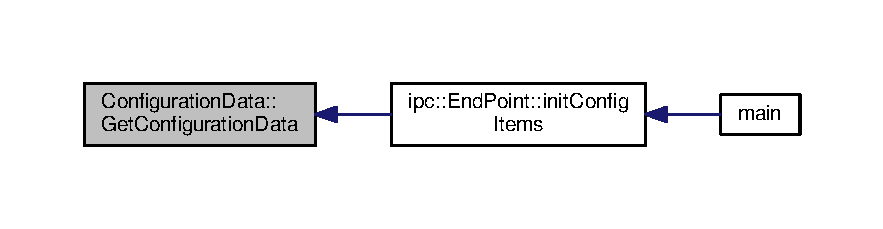
\includegraphics[width=350pt]{classConfigurationData_a85ef47317952a9369b474c8df2525322_icgraph}
\end{center}
\end{figure}


\index{Configuration\+Data@{Configuration\+Data}!get\+Configuration\+Data@{get\+Configuration\+Data}}
\index{get\+Configuration\+Data@{get\+Configuration\+Data}!Configuration\+Data@{Configuration\+Data}}
\subsubsection[{\texorpdfstring{get\+Configuration\+Data()}{getConfigurationData()}}]{\setlength{\rightskip}{0pt plus 5cm}{\bf configuration\+Data\+\_\+map\+\_\+t} Configuration\+Data\+::get\+Configuration\+Data (
\begin{DoxyParamCaption}
{}
\end{DoxyParamCaption}
)\hspace{0.3cm}{\ttfamily [inline]}}\hypertarget{classConfigurationData_a7a2e42c0440473858c382c39e3d66f3a}{}\label{classConfigurationData_a7a2e42c0440473858c382c39e3d66f3a}


Definition at line 213 of file Configuration\+Data.\+h.

\index{Configuration\+Data@{Configuration\+Data}!Get\+Configuration\+Data\+From\+Db@{Get\+Configuration\+Data\+From\+Db}}
\index{Get\+Configuration\+Data\+From\+Db@{Get\+Configuration\+Data\+From\+Db}!Configuration\+Data@{Configuration\+Data}}
\subsubsection[{\texorpdfstring{Get\+Configuration\+Data\+From\+Db(string svcname, bool is\+Success)}{GetConfigurationDataFromDb(string svcname, bool isSuccess)}}]{\setlength{\rightskip}{0pt plus 5cm}{\bf Dyn\+Cfg\+Intf\+Return\+Codes} Configuration\+Data\+::\+Get\+Configuration\+Data\+From\+Db (
\begin{DoxyParamCaption}
\item[{string}]{svcname, }
\item[{bool}]{is\+Success}
\end{DoxyParamCaption}
)}\hypertarget{classConfigurationData_aa5fd34a8fabbe045ec9b607a94fc021c}{}\label{classConfigurationData_aa5fd34a8fabbe045ec9b607a94fc021c}
\index{Configuration\+Data@{Configuration\+Data}!Get\+Configuration\+Data\+From\+File@{Get\+Configuration\+Data\+From\+File}}
\index{Get\+Configuration\+Data\+From\+File@{Get\+Configuration\+Data\+From\+File}!Configuration\+Data@{Configuration\+Data}}
\subsubsection[{\texorpdfstring{Get\+Configuration\+Data\+From\+File(const std\+::string file\+Name, bool is\+Success)}{GetConfigurationDataFromFile(const std::string fileName, bool isSuccess)}}]{\setlength{\rightskip}{0pt plus 5cm}{\bf Dyn\+Cfg\+Intf\+Return\+Codes} Configuration\+Data\+::\+Get\+Configuration\+Data\+From\+File (
\begin{DoxyParamCaption}
\item[{const std\+::string}]{file\+Name, }
\item[{bool}]{is\+Success}
\end{DoxyParamCaption}
)}\hypertarget{classConfigurationData_ae3be498bfc92a2162247810dfb37f6ec}{}\label{classConfigurationData_ae3be498bfc92a2162247810dfb37f6ec}
\index{Configuration\+Data@{Configuration\+Data}!Get\+Configuration\+Item\+Value@{Get\+Configuration\+Item\+Value}}
\index{Get\+Configuration\+Item\+Value@{Get\+Configuration\+Item\+Value}!Configuration\+Data@{Configuration\+Data}}
\subsubsection[{\texorpdfstring{Get\+Configuration\+Item\+Value(string str\+Group\+Name, string str\+Item\+Name, T t\+Def\+Item\+Value)}{GetConfigurationItemValue(string strGroupName, string strItemName, T tDefItemValue)}}]{\setlength{\rightskip}{0pt plus 5cm}template$<$typename T $>$ T Configuration\+Data\+::\+Get\+Configuration\+Item\+Value (
\begin{DoxyParamCaption}
\item[{string}]{str\+Group\+Name, }
\item[{string}]{str\+Item\+Name, }
\item[{T}]{t\+Def\+Item\+Value}
\end{DoxyParamCaption}
)}\hypertarget{classConfigurationData_a5960620b5e6e32d288157bb35860aa4d}{}\label{classConfigurationData_a5960620b5e6e32d288157bb35860aa4d}


Definition at line 275 of file Configuration\+Data.\+h.

\index{Configuration\+Data@{Configuration\+Data}!Get\+Data\+Source@{Get\+Data\+Source}}
\index{Get\+Data\+Source@{Get\+Data\+Source}!Configuration\+Data@{Configuration\+Data}}
\subsubsection[{\texorpdfstring{Get\+Data\+Source()}{GetDataSource()}}]{\setlength{\rightskip}{0pt plus 5cm}{\bf Data\+Source} Configuration\+Data\+::\+Get\+Data\+Source (
\begin{DoxyParamCaption}
{}
\end{DoxyParamCaption}
)\hspace{0.3cm}{\ttfamily [inline]}}\hypertarget{classConfigurationData_a10b79d03076c79b4e16aeed78f50a427}{}\label{classConfigurationData_a10b79d03076c79b4e16aeed78f50a427}


Definition at line 220 of file Configuration\+Data.\+h.

\index{Configuration\+Data@{Configuration\+Data}!get\+Double\+Type\+Item\+Value@{get\+Double\+Type\+Item\+Value}}
\index{get\+Double\+Type\+Item\+Value@{get\+Double\+Type\+Item\+Value}!Configuration\+Data@{Configuration\+Data}}
\subsubsection[{\texorpdfstring{get\+Double\+Type\+Item\+Value(string str\+Group\+Name, string str\+Item\+Name, double d\+Def\+Item\+Value=0.\+0)}{getDoubleTypeItemValue(string strGroupName, string strItemName, double dDefItemValue=0.0)}}]{\setlength{\rightskip}{0pt plus 5cm}double Configuration\+Data\+::get\+Double\+Type\+Item\+Value (
\begin{DoxyParamCaption}
\item[{string}]{str\+Group\+Name, }
\item[{string}]{str\+Item\+Name, }
\item[{double}]{d\+Def\+Item\+Value = {\ttfamily 0.0}}
\end{DoxyParamCaption}
)}\hypertarget{classConfigurationData_aa3255f642441d984e8963896a22eeb04}{}\label{classConfigurationData_aa3255f642441d984e8963896a22eeb04}
\index{Configuration\+Data@{Configuration\+Data}!Get\+File\+Name@{Get\+File\+Name}}
\index{Get\+File\+Name@{Get\+File\+Name}!Configuration\+Data@{Configuration\+Data}}
\subsubsection[{\texorpdfstring{Get\+File\+Name()}{GetFileName()}}]{\setlength{\rightskip}{0pt plus 5cm}const std\+::string\& Configuration\+Data\+::\+Get\+File\+Name (
\begin{DoxyParamCaption}
{}
\end{DoxyParamCaption}
)\hspace{0.3cm}{\ttfamily [inline]}}\hypertarget{classConfigurationData_abc7059c19e27c48a05ef4184c73a26bc}{}\label{classConfigurationData_abc7059c19e27c48a05ef4184c73a26bc}


Definition at line 232 of file Configuration\+Data.\+h.

\index{Configuration\+Data@{Configuration\+Data}!get\+Group\+Name@{get\+Group\+Name}}
\index{get\+Group\+Name@{get\+Group\+Name}!Configuration\+Data@{Configuration\+Data}}
\subsubsection[{\texorpdfstring{get\+Group\+Name(const std\+::string str\+Group\+\_\+c, vector$<$ Dynamic\+Config\+Item\+Data\+Struct $>$ \&vt\+\_\+config\+Data)}{getGroupName(const std::string strGroup_c, vector< DynamicConfigItemDataStruct > &vt_configData)}}]{\setlength{\rightskip}{0pt plus 5cm}bool Configuration\+Data\+::get\+Group\+Name (
\begin{DoxyParamCaption}
\item[{const std\+::string}]{str\+Group\+\_\+c, }
\item[{vector$<$ {\bf Dynamic\+Config\+Item\+Data\+Struct} $>$ \&}]{vt\+\_\+config\+Data}
\end{DoxyParamCaption}
)}\hypertarget{classConfigurationData_a37a40d143e56aa3577cace34049091df}{}\label{classConfigurationData_a37a40d143e56aa3577cace34049091df}
\index{Configuration\+Data@{Configuration\+Data}!get\+Int\+Type\+Item\+Value@{get\+Int\+Type\+Item\+Value}}
\index{get\+Int\+Type\+Item\+Value@{get\+Int\+Type\+Item\+Value}!Configuration\+Data@{Configuration\+Data}}
\subsubsection[{\texorpdfstring{get\+Int\+Type\+Item\+Value(string str\+Group\+Name, string str\+Item\+Name, int n\+Def\+Item\+Value=0)}{getIntTypeItemValue(string strGroupName, string strItemName, int nDefItemValue=0)}}]{\setlength{\rightskip}{0pt plus 5cm}int Configuration\+Data\+::get\+Int\+Type\+Item\+Value (
\begin{DoxyParamCaption}
\item[{string}]{str\+Group\+Name, }
\item[{string}]{str\+Item\+Name, }
\item[{int}]{n\+Def\+Item\+Value = {\ttfamily 0}}
\end{DoxyParamCaption}
)}\hypertarget{classConfigurationData_a54bb3e76dfb9e720bbcb41a277e1aee1}{}\label{classConfigurationData_a54bb3e76dfb9e720bbcb41a277e1aee1}


Here is the caller graph for this function\+:
\nopagebreak
\begin{figure}[H]
\begin{center}
\leavevmode
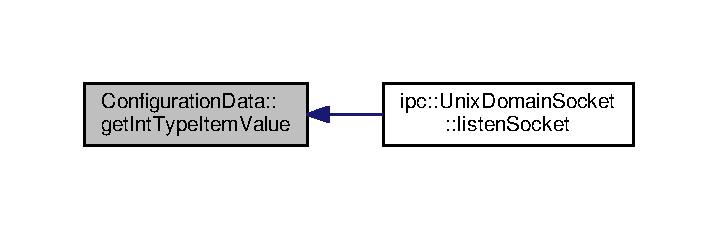
\includegraphics[width=344pt]{classConfigurationData_a54bb3e76dfb9e720bbcb41a277e1aee1_icgraph}
\end{center}
\end{figure}


\index{Configuration\+Data@{Configuration\+Data}!get\+Item\+Name\+Found@{get\+Item\+Name\+Found}}
\index{get\+Item\+Name\+Found@{get\+Item\+Name\+Found}!Configuration\+Data@{Configuration\+Data}}
\subsubsection[{\texorpdfstring{get\+Item\+Name\+Found()}{getItemNameFound()}}]{\setlength{\rightskip}{0pt plus 5cm}bool Configuration\+Data\+::get\+Item\+Name\+Found (
\begin{DoxyParamCaption}
{}
\end{DoxyParamCaption}
)\hspace{0.3cm}{\ttfamily [inline]}}\hypertarget{classConfigurationData_a7c04864007d1a78c1881b1ab83d78698}{}\label{classConfigurationData_a7c04864007d1a78c1881b1ab83d78698}


Definition at line 207 of file Configuration\+Data.\+h.

\index{Configuration\+Data@{Configuration\+Data}!get\+Item\+Value\+String\+List@{get\+Item\+Value\+String\+List}}
\index{get\+Item\+Value\+String\+List@{get\+Item\+Value\+String\+List}!Configuration\+Data@{Configuration\+Data}}
\subsubsection[{\texorpdfstring{get\+Item\+Value\+String\+List(string str\+Group\+Name, string str\+Item\+Name)}{getItemValueStringList(string strGroupName, string strItemName)}}]{\setlength{\rightskip}{0pt plus 5cm}std\+::vector$<$std\+::string$>$\& Configuration\+Data\+::get\+Item\+Value\+String\+List (
\begin{DoxyParamCaption}
\item[{string}]{str\+Group\+Name, }
\item[{string}]{str\+Item\+Name}
\end{DoxyParamCaption}
)}\hypertarget{classConfigurationData_af68323f3fea60118d8150ad469bd2a0a}{}\label{classConfigurationData_af68323f3fea60118d8150ad469bd2a0a}
\index{Configuration\+Data@{Configuration\+Data}!get\+Long\+Type\+Item\+Value@{get\+Long\+Type\+Item\+Value}}
\index{get\+Long\+Type\+Item\+Value@{get\+Long\+Type\+Item\+Value}!Configuration\+Data@{Configuration\+Data}}
\subsubsection[{\texorpdfstring{get\+Long\+Type\+Item\+Value(string str\+Group\+Name, string str\+Item\+Name, long l\+Def\+Item\+Value=0)}{getLongTypeItemValue(string strGroupName, string strItemName, long lDefItemValue=0)}}]{\setlength{\rightskip}{0pt plus 5cm}long Configuration\+Data\+::get\+Long\+Type\+Item\+Value (
\begin{DoxyParamCaption}
\item[{string}]{str\+Group\+Name, }
\item[{string}]{str\+Item\+Name, }
\item[{long}]{l\+Def\+Item\+Value = {\ttfamily 0}}
\end{DoxyParamCaption}
)}\hypertarget{classConfigurationData_ace8acd6f1471ffc98cc2df5e526d7e3a}{}\label{classConfigurationData_ace8acd6f1471ffc98cc2df5e526d7e3a}
\index{Configuration\+Data@{Configuration\+Data}!get\+Name\+Value\+List@{get\+Name\+Value\+List}}
\index{get\+Name\+Value\+List@{get\+Name\+Value\+List}!Configuration\+Data@{Configuration\+Data}}
\subsubsection[{\texorpdfstring{get\+Name\+Value\+List(string str\+Group\+Name)}{getNameValueList(string strGroupName)}}]{\setlength{\rightskip}{0pt plus 5cm}std\+::vector$<$std\+::pair$<$std\+::string, std\+::string$>$ $>$ Configuration\+Data\+::get\+Name\+Value\+List (
\begin{DoxyParamCaption}
\item[{string}]{str\+Group\+Name}
\end{DoxyParamCaption}
)}\hypertarget{classConfigurationData_acab5cb404d738f84daed25f604f692e4}{}\label{classConfigurationData_acab5cb404d738f84daed25f604f692e4}
\index{Configuration\+Data@{Configuration\+Data}!Get\+Service\+Name@{Get\+Service\+Name}}
\index{Get\+Service\+Name@{Get\+Service\+Name}!Configuration\+Data@{Configuration\+Data}}
\subsubsection[{\texorpdfstring{Get\+Service\+Name()}{GetServiceName()}}]{\setlength{\rightskip}{0pt plus 5cm}const std\+::string\& Configuration\+Data\+::\+Get\+Service\+Name (
\begin{DoxyParamCaption}
{}
\end{DoxyParamCaption}
)\hspace{0.3cm}{\ttfamily [inline]}}\hypertarget{classConfigurationData_a1deecfa52d87b2cfedf59390813bd2b3}{}\label{classConfigurationData_a1deecfa52d87b2cfedf59390813bd2b3}


Definition at line 243 of file Configuration\+Data.\+h.

\index{Configuration\+Data@{Configuration\+Data}!get\+String\+Type\+Item\+Value@{get\+String\+Type\+Item\+Value}}
\index{get\+String\+Type\+Item\+Value@{get\+String\+Type\+Item\+Value}!Configuration\+Data@{Configuration\+Data}}
\subsubsection[{\texorpdfstring{get\+String\+Type\+Item\+Value(string str\+Group\+Name, string str\+Item\+Name, string str\+Def\+Item\+Value="""")}{getStringTypeItemValue(string strGroupName, string strItemName, string strDefItemValue="")}}]{\setlength{\rightskip}{0pt plus 5cm}string Configuration\+Data\+::get\+String\+Type\+Item\+Value (
\begin{DoxyParamCaption}
\item[{string}]{str\+Group\+Name, }
\item[{string}]{str\+Item\+Name, }
\item[{string}]{str\+Def\+Item\+Value = {\ttfamily \char`\"{}\char`\"{}}}
\end{DoxyParamCaption}
)}\hypertarget{classConfigurationData_a59866f345224cbf203c835e0693771b9}{}\label{classConfigurationData_a59866f345224cbf203c835e0693771b9}


Here is the caller graph for this function\+:
\nopagebreak
\begin{figure}[H]
\begin{center}
\leavevmode
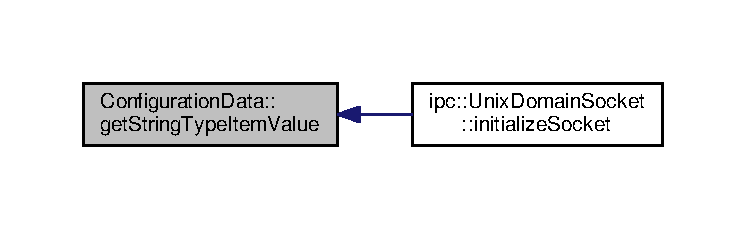
\includegraphics[width=350pt]{classConfigurationData_a59866f345224cbf203c835e0693771b9_icgraph}
\end{center}
\end{figure}


\index{Configuration\+Data@{Configuration\+Data}!print\+Configuration\+Data@{print\+Configuration\+Data}}
\index{print\+Configuration\+Data@{print\+Configuration\+Data}!Configuration\+Data@{Configuration\+Data}}
\subsubsection[{\texorpdfstring{print\+Configuration\+Data()}{printConfigurationData()}}]{\setlength{\rightskip}{0pt plus 5cm}bool Configuration\+Data\+::print\+Configuration\+Data (
\begin{DoxyParamCaption}
{}
\end{DoxyParamCaption}
)}\hypertarget{classConfigurationData_a93380d92256f8798651a07fce30f7d83}{}\label{classConfigurationData_a93380d92256f8798651a07fce30f7d83}
\index{Configuration\+Data@{Configuration\+Data}!Set\+Data\+Source@{Set\+Data\+Source}}
\index{Set\+Data\+Source@{Set\+Data\+Source}!Configuration\+Data@{Configuration\+Data}}
\subsubsection[{\texorpdfstring{Set\+Data\+Source(\+Data\+Source source)}{SetDataSource(DataSource source)}}]{\setlength{\rightskip}{0pt plus 5cm}void Configuration\+Data\+::\+Set\+Data\+Source (
\begin{DoxyParamCaption}
\item[{{\bf Data\+Source}}]{source}
\end{DoxyParamCaption}
)\hspace{0.3cm}{\ttfamily [inline]}}\hypertarget{classConfigurationData_ac5288ab51744fc8697a24d2663136916}{}\label{classConfigurationData_ac5288ab51744fc8697a24d2663136916}


Definition at line 226 of file Configuration\+Data.\+h.



Here is the caller graph for this function\+:
\nopagebreak
\begin{figure}[H]
\begin{center}
\leavevmode
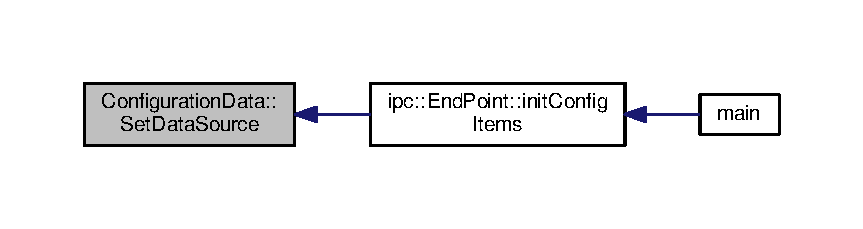
\includegraphics[width=350pt]{classConfigurationData_ac5288ab51744fc8697a24d2663136916_icgraph}
\end{center}
\end{figure}


\index{Configuration\+Data@{Configuration\+Data}!Set\+File\+Name@{Set\+File\+Name}}
\index{Set\+File\+Name@{Set\+File\+Name}!Configuration\+Data@{Configuration\+Data}}
\subsubsection[{\texorpdfstring{Set\+File\+Name(string str\+File\+Name)}{SetFileName(string strFileName)}}]{\setlength{\rightskip}{0pt plus 5cm}void Configuration\+Data\+::\+Set\+File\+Name (
\begin{DoxyParamCaption}
\item[{string}]{str\+File\+Name}
\end{DoxyParamCaption}
)\hspace{0.3cm}{\ttfamily [inline]}}\hypertarget{classConfigurationData_a54f43e41906262c4a336b370a4f1726c}{}\label{classConfigurationData_a54f43e41906262c4a336b370a4f1726c}


Definition at line 237 of file Configuration\+Data.\+h.



Here is the caller graph for this function\+:
\nopagebreak
\begin{figure}[H]
\begin{center}
\leavevmode
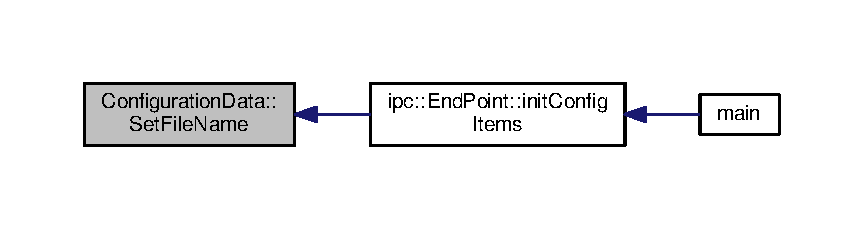
\includegraphics[width=350pt]{classConfigurationData_a54f43e41906262c4a336b370a4f1726c_icgraph}
\end{center}
\end{figure}


\index{Configuration\+Data@{Configuration\+Data}!Set\+Service\+Name@{Set\+Service\+Name}}
\index{Set\+Service\+Name@{Set\+Service\+Name}!Configuration\+Data@{Configuration\+Data}}
\subsubsection[{\texorpdfstring{Set\+Service\+Name(string str\+Svc\+Name)}{SetServiceName(string strSvcName)}}]{\setlength{\rightskip}{0pt plus 5cm}void Configuration\+Data\+::\+Set\+Service\+Name (
\begin{DoxyParamCaption}
\item[{string}]{str\+Svc\+Name}
\end{DoxyParamCaption}
)\hspace{0.3cm}{\ttfamily [inline]}}\hypertarget{classConfigurationData_aeaa0566bed9b1c41ae77a363a811e1ce}{}\label{classConfigurationData_aeaa0566bed9b1c41ae77a363a811e1ce}


Definition at line 248 of file Configuration\+Data.\+h.



Here is the caller graph for this function\+:
\nopagebreak
\begin{figure}[H]
\begin{center}
\leavevmode
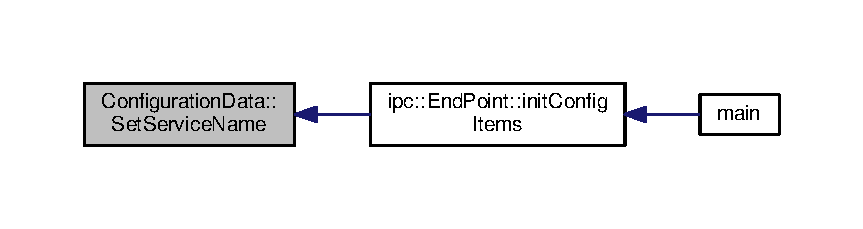
\includegraphics[width=350pt]{classConfigurationData_aeaa0566bed9b1c41ae77a363a811e1ce_icgraph}
\end{center}
\end{figure}




\subsection{Member Data Documentation}
\index{Configuration\+Data@{Configuration\+Data}!configuration\+Data\+\_\+map@{configuration\+Data\+\_\+map}}
\index{configuration\+Data\+\_\+map@{configuration\+Data\+\_\+map}!Configuration\+Data@{Configuration\+Data}}
\subsubsection[{\texorpdfstring{configuration\+Data\+\_\+map}{configurationData_map}}]{\setlength{\rightskip}{0pt plus 5cm}{\bf configuration\+Data\+\_\+map\+\_\+t} Configuration\+Data\+::configuration\+Data\+\_\+map\hspace{0.3cm}{\ttfamily [static]}}\hypertarget{classConfigurationData_a7068df8bceb0fd7e24abde430532eeca}{}\label{classConfigurationData_a7068df8bceb0fd7e24abde430532eeca}


Definition at line 41 of file Configuration\+Data.\+h.

\index{Configuration\+Data@{Configuration\+Data}!m\+\_\+b\+Item\+Found\+Flag@{m\+\_\+b\+Item\+Found\+Flag}}
\index{m\+\_\+b\+Item\+Found\+Flag@{m\+\_\+b\+Item\+Found\+Flag}!Configuration\+Data@{Configuration\+Data}}
\subsubsection[{\texorpdfstring{m\+\_\+b\+Item\+Found\+Flag}{m_bItemFoundFlag}}]{\setlength{\rightskip}{0pt plus 5cm}bool Configuration\+Data\+::m\+\_\+b\+Item\+Found\+Flag\hspace{0.3cm}{\ttfamily [protected]}}\hypertarget{classConfigurationData_a358d8d3d441e31872a9f52a5dd0a8943}{}\label{classConfigurationData_a358d8d3d441e31872a9f52a5dd0a8943}


Definition at line 259 of file Configuration\+Data.\+h.

\index{Configuration\+Data@{Configuration\+Data}!m\+\_\+data\+Source@{m\+\_\+data\+Source}}
\index{m\+\_\+data\+Source@{m\+\_\+data\+Source}!Configuration\+Data@{Configuration\+Data}}
\subsubsection[{\texorpdfstring{m\+\_\+data\+Source}{m_dataSource}}]{\setlength{\rightskip}{0pt plus 5cm}{\bf Data\+Source} Configuration\+Data\+::m\+\_\+data\+Source\hspace{0.3cm}{\ttfamily [protected]}}\hypertarget{classConfigurationData_a76fde55e5e58cd5726449bee19c378dd}{}\label{classConfigurationData_a76fde55e5e58cd5726449bee19c378dd}


Definition at line 255 of file Configuration\+Data.\+h.

\index{Configuration\+Data@{Configuration\+Data}!m\+\_\+str\+File\+Name@{m\+\_\+str\+File\+Name}}
\index{m\+\_\+str\+File\+Name@{m\+\_\+str\+File\+Name}!Configuration\+Data@{Configuration\+Data}}
\subsubsection[{\texorpdfstring{m\+\_\+str\+File\+Name}{m_strFileName}}]{\setlength{\rightskip}{0pt plus 5cm}string Configuration\+Data\+::m\+\_\+str\+File\+Name\hspace{0.3cm}{\ttfamily [protected]}}\hypertarget{classConfigurationData_a3c2246db7a0a2cfa91081e91a98625df}{}\label{classConfigurationData_a3c2246db7a0a2cfa91081e91a98625df}


Definition at line 257 of file Configuration\+Data.\+h.

\index{Configuration\+Data@{Configuration\+Data}!m\+\_\+str\+Service\+Name@{m\+\_\+str\+Service\+Name}}
\index{m\+\_\+str\+Service\+Name@{m\+\_\+str\+Service\+Name}!Configuration\+Data@{Configuration\+Data}}
\subsubsection[{\texorpdfstring{m\+\_\+str\+Service\+Name}{m_strServiceName}}]{\setlength{\rightskip}{0pt plus 5cm}string Configuration\+Data\+::m\+\_\+str\+Service\+Name\hspace{0.3cm}{\ttfamily [protected]}}\hypertarget{classConfigurationData_aae2da98258156ab8a7b4884694d5cea7}{}\label{classConfigurationData_aae2da98258156ab8a7b4884694d5cea7}


Definition at line 256 of file Configuration\+Data.\+h.

\index{Configuration\+Data@{Configuration\+Data}!m\+\_\+sz\+Error\+Message@{m\+\_\+sz\+Error\+Message}}
\index{m\+\_\+sz\+Error\+Message@{m\+\_\+sz\+Error\+Message}!Configuration\+Data@{Configuration\+Data}}
\subsubsection[{\texorpdfstring{m\+\_\+sz\+Error\+Message}{m_szErrorMessage}}]{\setlength{\rightskip}{0pt plus 5cm}char Configuration\+Data\+::m\+\_\+sz\+Error\+Message\mbox{[}512\mbox{]}}\hypertarget{classConfigurationData_aefb528ceef393a3d4a016ab52fca5c0b}{}\label{classConfigurationData_aefb528ceef393a3d4a016ab52fca5c0b}


Definition at line 38 of file Configuration\+Data.\+h.



The documentation for this class was generated from the following file\+:\begin{DoxyCompactItemize}
\item 
D\+Y\+N\+\_\+\+C\+O\+N\+F\+I\+G/include/\hyperlink{ConfigurationData_8h}{Configuration\+Data.\+h}\end{DoxyCompactItemize}

\hypertarget{classConfigurationDataFromDatabase}{}\section{Configuration\+Data\+From\+Database Class Reference}
\label{classConfigurationDataFromDatabase}\index{Configuration\+Data\+From\+Database@{Configuration\+Data\+From\+Database}}


{\ttfamily \#include $<$Configuration\+Data\+From\+Database.\+h$>$}

\subsection*{Public Member Functions}
\begin{DoxyCompactItemize}
\item 
\hyperlink{classConfigurationDataFromDatabase_a6c0e423623ede29421d9678288decc21}{Configuration\+Data\+From\+Database} ()
\item 
\hyperlink{classConfigurationDataFromDatabase_a2d769374c9a11cb9a2b4678a89995da9}{$\sim$\+Configuration\+Data\+From\+Database} ()
\item 
map$<$ string, vector$<$ \hyperlink{structDynamicConfigItemDataStruct}{Dynamic\+Config\+Item\+Data\+Struct} $>$ $>$ \hyperlink{classConfigurationDataFromDatabase_a5f9c07b2e4bf331a2e06c3ac226b2dd7}{Retrieve\+Service\+Configuration\+Data} (string service\+Name, bool \&is\+Success)
\end{DoxyCompactItemize}
\subsection*{Public Attributes}
\begin{DoxyCompactItemize}
\item 
char \hyperlink{classConfigurationDataFromDatabase_aac7ca30370d501a0a55681c6174f906b}{m\+\_\+sz\+Error\+Message} \mbox{[}\hyperlink{ConfigurationDataFromDatabase_8h_a6e392370bd440c3edd8c168172e1ea08}{max\+\_\+msg\+\_\+size\+\_\+c}\mbox{]}
\item 
long \hyperlink{classConfigurationDataFromDatabase_a20f590ac28d74a441f0cecedff273392}{m\+\_\+dw\+Error\+Code}
\end{DoxyCompactItemize}


\subsection{Detailed Description}


Definition at line 22 of file Configuration\+Data\+From\+Database.\+h.



\subsection{Constructor \& Destructor Documentation}
\index{Configuration\+Data\+From\+Database@{Configuration\+Data\+From\+Database}!Configuration\+Data\+From\+Database@{Configuration\+Data\+From\+Database}}
\index{Configuration\+Data\+From\+Database@{Configuration\+Data\+From\+Database}!Configuration\+Data\+From\+Database@{Configuration\+Data\+From\+Database}}
\subsubsection[{\texorpdfstring{Configuration\+Data\+From\+Database()}{ConfigurationDataFromDatabase()}}]{\setlength{\rightskip}{0pt plus 5cm}Configuration\+Data\+From\+Database\+::\+Configuration\+Data\+From\+Database (
\begin{DoxyParamCaption}
{}
\end{DoxyParamCaption}
)}\hypertarget{classConfigurationDataFromDatabase_a6c0e423623ede29421d9678288decc21}{}\label{classConfigurationDataFromDatabase_a6c0e423623ede29421d9678288decc21}
\index{Configuration\+Data\+From\+Database@{Configuration\+Data\+From\+Database}!````~Configuration\+Data\+From\+Database@{$\sim$\+Configuration\+Data\+From\+Database}}
\index{````~Configuration\+Data\+From\+Database@{$\sim$\+Configuration\+Data\+From\+Database}!Configuration\+Data\+From\+Database@{Configuration\+Data\+From\+Database}}
\subsubsection[{\texorpdfstring{$\sim$\+Configuration\+Data\+From\+Database()}{~ConfigurationDataFromDatabase()}}]{\setlength{\rightskip}{0pt plus 5cm}Configuration\+Data\+From\+Database\+::$\sim$\+Configuration\+Data\+From\+Database (
\begin{DoxyParamCaption}
{}
\end{DoxyParamCaption}
)}\hypertarget{classConfigurationDataFromDatabase_a2d769374c9a11cb9a2b4678a89995da9}{}\label{classConfigurationDataFromDatabase_a2d769374c9a11cb9a2b4678a89995da9}


\subsection{Member Function Documentation}
\index{Configuration\+Data\+From\+Database@{Configuration\+Data\+From\+Database}!Retrieve\+Service\+Configuration\+Data@{Retrieve\+Service\+Configuration\+Data}}
\index{Retrieve\+Service\+Configuration\+Data@{Retrieve\+Service\+Configuration\+Data}!Configuration\+Data\+From\+Database@{Configuration\+Data\+From\+Database}}
\subsubsection[{\texorpdfstring{Retrieve\+Service\+Configuration\+Data(string service\+Name, bool \&is\+Success)}{RetrieveServiceConfigurationData(string serviceName, bool &isSuccess)}}]{\setlength{\rightskip}{0pt plus 5cm}map$<$string, vector $<${\bf Dynamic\+Config\+Item\+Data\+Struct}$>$ $>$ Configuration\+Data\+From\+Database\+::\+Retrieve\+Service\+Configuration\+Data (
\begin{DoxyParamCaption}
\item[{string}]{service\+Name, }
\item[{bool \&}]{is\+Success}
\end{DoxyParamCaption}
)}\hypertarget{classConfigurationDataFromDatabase_a5f9c07b2e4bf331a2e06c3ac226b2dd7}{}\label{classConfigurationDataFromDatabase_a5f9c07b2e4bf331a2e06c3ac226b2dd7}


\subsection{Member Data Documentation}
\index{Configuration\+Data\+From\+Database@{Configuration\+Data\+From\+Database}!m\+\_\+dw\+Error\+Code@{m\+\_\+dw\+Error\+Code}}
\index{m\+\_\+dw\+Error\+Code@{m\+\_\+dw\+Error\+Code}!Configuration\+Data\+From\+Database@{Configuration\+Data\+From\+Database}}
\subsubsection[{\texorpdfstring{m\+\_\+dw\+Error\+Code}{m_dwErrorCode}}]{\setlength{\rightskip}{0pt plus 5cm}long Configuration\+Data\+From\+Database\+::m\+\_\+dw\+Error\+Code}\hypertarget{classConfigurationDataFromDatabase_a20f590ac28d74a441f0cecedff273392}{}\label{classConfigurationDataFromDatabase_a20f590ac28d74a441f0cecedff273392}


Definition at line 26 of file Configuration\+Data\+From\+Database.\+h.

\index{Configuration\+Data\+From\+Database@{Configuration\+Data\+From\+Database}!m\+\_\+sz\+Error\+Message@{m\+\_\+sz\+Error\+Message}}
\index{m\+\_\+sz\+Error\+Message@{m\+\_\+sz\+Error\+Message}!Configuration\+Data\+From\+Database@{Configuration\+Data\+From\+Database}}
\subsubsection[{\texorpdfstring{m\+\_\+sz\+Error\+Message}{m_szErrorMessage}}]{\setlength{\rightskip}{0pt plus 5cm}char Configuration\+Data\+From\+Database\+::m\+\_\+sz\+Error\+Message\mbox{[}{\bf max\+\_\+msg\+\_\+size\+\_\+c}\mbox{]}}\hypertarget{classConfigurationDataFromDatabase_aac7ca30370d501a0a55681c6174f906b}{}\label{classConfigurationDataFromDatabase_aac7ca30370d501a0a55681c6174f906b}


Definition at line 25 of file Configuration\+Data\+From\+Database.\+h.



The documentation for this class was generated from the following file\+:\begin{DoxyCompactItemize}
\item 
D\+Y\+N\+\_\+\+C\+O\+N\+F\+I\+G/include/\hyperlink{ConfigurationDataFromDatabase_8h}{Configuration\+Data\+From\+Database.\+h}\end{DoxyCompactItemize}

\hypertarget{classDatabaseDetails}{}\section{Database\+Details Class Reference}
\label{classDatabaseDetails}\index{Database\+Details@{Database\+Details}}


{\ttfamily \#include $<$Database\+Details.\+h$>$}

\subsection*{Public Member Functions}
\begin{DoxyCompactItemize}
\item 
\hyperlink{classDatabaseDetails_acabeafc7ed16f5a2157848bad8e9e7aa}{Database\+Details} ()
\item 
virtual \hyperlink{classDatabaseDetails_a869768858f75283b579dd5c62b05ce71}{$\sim$\+Database\+Details} ()
\item 
string \hyperlink{classDatabaseDetails_aa14ce03e41c3bb2c78f2d455b7423436}{get\+Database\+Name} () const 
\item 
void \hyperlink{classDatabaseDetails_ad5a8adc1d2e84c83aa0860cd63911393}{set\+Database\+Name} (string database\+Name)
\item 
string \hyperlink{classDatabaseDetails_aff9d9a580f67e985b0dee76b697fa57c}{get\+Password} () const 
\item 
void \hyperlink{classDatabaseDetails_a61b082a9006613de2453bfab67f1af9e}{set\+Password} (string password)
\item 
string \hyperlink{classDatabaseDetails_a3bc6aa0cab0547109277e5e6179fe24c}{get\+Tag\+Name} () const 
\item 
void \hyperlink{classDatabaseDetails_afadd6c964135607f0daaeae2cec64497}{set\+Tag\+Name} (string tag\+Name)
\item 
string \hyperlink{classDatabaseDetails_ad8153b502d603be68b389a0aca7d2b15}{get\+User\+Name} () const 
\item 
void \hyperlink{classDatabaseDetails_a2070515ac65842cbfe50d8e7423f6952}{set\+User\+Name} (string user\+Name)
\item 
bool \hyperlink{classDatabaseDetails_a1d16c8e4021ac65b09e3cd51d12b1f36}{is\+Connected} () const 
\item 
void \hyperlink{classDatabaseDetails_a59395315dd39566ecef24b99e9232ce0}{set\+Connected} (bool connected)
\end{DoxyCompactItemize}


\subsection{Detailed Description}


Definition at line 15 of file Database\+Details.\+h.



\subsection{Constructor \& Destructor Documentation}
\index{Database\+Details@{Database\+Details}!Database\+Details@{Database\+Details}}
\index{Database\+Details@{Database\+Details}!Database\+Details@{Database\+Details}}
\subsubsection[{\texorpdfstring{Database\+Details()}{DatabaseDetails()}}]{\setlength{\rightskip}{0pt plus 5cm}Database\+Details\+::\+Database\+Details (
\begin{DoxyParamCaption}
{}
\end{DoxyParamCaption}
)}\hypertarget{classDatabaseDetails_acabeafc7ed16f5a2157848bad8e9e7aa}{}\label{classDatabaseDetails_acabeafc7ed16f5a2157848bad8e9e7aa}
\index{Database\+Details@{Database\+Details}!````~Database\+Details@{$\sim$\+Database\+Details}}
\index{````~Database\+Details@{$\sim$\+Database\+Details}!Database\+Details@{Database\+Details}}
\subsubsection[{\texorpdfstring{$\sim$\+Database\+Details()}{~DatabaseDetails()}}]{\setlength{\rightskip}{0pt plus 5cm}virtual Database\+Details\+::$\sim$\+Database\+Details (
\begin{DoxyParamCaption}
{}
\end{DoxyParamCaption}
)\hspace{0.3cm}{\ttfamily [virtual]}}\hypertarget{classDatabaseDetails_a869768858f75283b579dd5c62b05ce71}{}\label{classDatabaseDetails_a869768858f75283b579dd5c62b05ce71}


\subsection{Member Function Documentation}
\index{Database\+Details@{Database\+Details}!get\+Database\+Name@{get\+Database\+Name}}
\index{get\+Database\+Name@{get\+Database\+Name}!Database\+Details@{Database\+Details}}
\subsubsection[{\texorpdfstring{get\+Database\+Name() const }{getDatabaseName() const }}]{\setlength{\rightskip}{0pt plus 5cm}string Database\+Details\+::get\+Database\+Name (
\begin{DoxyParamCaption}
{}
\end{DoxyParamCaption}
) const}\hypertarget{classDatabaseDetails_aa14ce03e41c3bb2c78f2d455b7423436}{}\label{classDatabaseDetails_aa14ce03e41c3bb2c78f2d455b7423436}
\index{Database\+Details@{Database\+Details}!get\+Password@{get\+Password}}
\index{get\+Password@{get\+Password}!Database\+Details@{Database\+Details}}
\subsubsection[{\texorpdfstring{get\+Password() const }{getPassword() const }}]{\setlength{\rightskip}{0pt plus 5cm}string Database\+Details\+::get\+Password (
\begin{DoxyParamCaption}
{}
\end{DoxyParamCaption}
) const}\hypertarget{classDatabaseDetails_aff9d9a580f67e985b0dee76b697fa57c}{}\label{classDatabaseDetails_aff9d9a580f67e985b0dee76b697fa57c}
\index{Database\+Details@{Database\+Details}!get\+Tag\+Name@{get\+Tag\+Name}}
\index{get\+Tag\+Name@{get\+Tag\+Name}!Database\+Details@{Database\+Details}}
\subsubsection[{\texorpdfstring{get\+Tag\+Name() const }{getTagName() const }}]{\setlength{\rightskip}{0pt plus 5cm}string Database\+Details\+::get\+Tag\+Name (
\begin{DoxyParamCaption}
{}
\end{DoxyParamCaption}
) const}\hypertarget{classDatabaseDetails_a3bc6aa0cab0547109277e5e6179fe24c}{}\label{classDatabaseDetails_a3bc6aa0cab0547109277e5e6179fe24c}
\index{Database\+Details@{Database\+Details}!get\+User\+Name@{get\+User\+Name}}
\index{get\+User\+Name@{get\+User\+Name}!Database\+Details@{Database\+Details}}
\subsubsection[{\texorpdfstring{get\+User\+Name() const }{getUserName() const }}]{\setlength{\rightskip}{0pt plus 5cm}string Database\+Details\+::get\+User\+Name (
\begin{DoxyParamCaption}
{}
\end{DoxyParamCaption}
) const}\hypertarget{classDatabaseDetails_ad8153b502d603be68b389a0aca7d2b15}{}\label{classDatabaseDetails_ad8153b502d603be68b389a0aca7d2b15}
\index{Database\+Details@{Database\+Details}!is\+Connected@{is\+Connected}}
\index{is\+Connected@{is\+Connected}!Database\+Details@{Database\+Details}}
\subsubsection[{\texorpdfstring{is\+Connected() const }{isConnected() const }}]{\setlength{\rightskip}{0pt plus 5cm}bool Database\+Details\+::is\+Connected (
\begin{DoxyParamCaption}
{}
\end{DoxyParamCaption}
) const}\hypertarget{classDatabaseDetails_a1d16c8e4021ac65b09e3cd51d12b1f36}{}\label{classDatabaseDetails_a1d16c8e4021ac65b09e3cd51d12b1f36}
\index{Database\+Details@{Database\+Details}!set\+Connected@{set\+Connected}}
\index{set\+Connected@{set\+Connected}!Database\+Details@{Database\+Details}}
\subsubsection[{\texorpdfstring{set\+Connected(bool connected)}{setConnected(bool connected)}}]{\setlength{\rightskip}{0pt plus 5cm}void Database\+Details\+::set\+Connected (
\begin{DoxyParamCaption}
\item[{bool}]{connected}
\end{DoxyParamCaption}
)}\hypertarget{classDatabaseDetails_a59395315dd39566ecef24b99e9232ce0}{}\label{classDatabaseDetails_a59395315dd39566ecef24b99e9232ce0}
\index{Database\+Details@{Database\+Details}!set\+Database\+Name@{set\+Database\+Name}}
\index{set\+Database\+Name@{set\+Database\+Name}!Database\+Details@{Database\+Details}}
\subsubsection[{\texorpdfstring{set\+Database\+Name(string database\+Name)}{setDatabaseName(string databaseName)}}]{\setlength{\rightskip}{0pt plus 5cm}void Database\+Details\+::set\+Database\+Name (
\begin{DoxyParamCaption}
\item[{string}]{database\+Name}
\end{DoxyParamCaption}
)}\hypertarget{classDatabaseDetails_ad5a8adc1d2e84c83aa0860cd63911393}{}\label{classDatabaseDetails_ad5a8adc1d2e84c83aa0860cd63911393}
\index{Database\+Details@{Database\+Details}!set\+Password@{set\+Password}}
\index{set\+Password@{set\+Password}!Database\+Details@{Database\+Details}}
\subsubsection[{\texorpdfstring{set\+Password(string password)}{setPassword(string password)}}]{\setlength{\rightskip}{0pt plus 5cm}void Database\+Details\+::set\+Password (
\begin{DoxyParamCaption}
\item[{string}]{password}
\end{DoxyParamCaption}
)}\hypertarget{classDatabaseDetails_a61b082a9006613de2453bfab67f1af9e}{}\label{classDatabaseDetails_a61b082a9006613de2453bfab67f1af9e}
\index{Database\+Details@{Database\+Details}!set\+Tag\+Name@{set\+Tag\+Name}}
\index{set\+Tag\+Name@{set\+Tag\+Name}!Database\+Details@{Database\+Details}}
\subsubsection[{\texorpdfstring{set\+Tag\+Name(string tag\+Name)}{setTagName(string tagName)}}]{\setlength{\rightskip}{0pt plus 5cm}void Database\+Details\+::set\+Tag\+Name (
\begin{DoxyParamCaption}
\item[{string}]{tag\+Name}
\end{DoxyParamCaption}
)}\hypertarget{classDatabaseDetails_afadd6c964135607f0daaeae2cec64497}{}\label{classDatabaseDetails_afadd6c964135607f0daaeae2cec64497}
\index{Database\+Details@{Database\+Details}!set\+User\+Name@{set\+User\+Name}}
\index{set\+User\+Name@{set\+User\+Name}!Database\+Details@{Database\+Details}}
\subsubsection[{\texorpdfstring{set\+User\+Name(string user\+Name)}{setUserName(string userName)}}]{\setlength{\rightskip}{0pt plus 5cm}void Database\+Details\+::set\+User\+Name (
\begin{DoxyParamCaption}
\item[{string}]{user\+Name}
\end{DoxyParamCaption}
)}\hypertarget{classDatabaseDetails_a2070515ac65842cbfe50d8e7423f6952}{}\label{classDatabaseDetails_a2070515ac65842cbfe50d8e7423f6952}


The documentation for this class was generated from the following file\+:\begin{DoxyCompactItemize}
\item 
D\+Y\+N\+\_\+\+C\+O\+N\+F\+I\+G/include/\hyperlink{DatabaseDetails_8h}{Database\+Details.\+h}\end{DoxyCompactItemize}

\hypertarget{structDynamicConfigItemDataStruct}{}\section{Dynamic\+Config\+Item\+Data\+Struct Struct Reference}
\label{structDynamicConfigItemDataStruct}\index{Dynamic\+Config\+Item\+Data\+Struct@{Dynamic\+Config\+Item\+Data\+Struct}}


{\ttfamily \#include $<$Dynamic\+Config\+Item\+Data\+Struct.\+h$>$}

\subsection*{Public Attributes}
\begin{DoxyCompactItemize}
\item 
char \hyperlink{structDynamicConfigItemDataStruct_a4959e12c0fab44e54a8edc4dde9e6386}{conf\+\_\+item\+\_\+value} \mbox{[}\hyperlink{DynamicConfigItemDataStruct_8h_a856963f31e35df3fa9c1dc12c397f6be}{max\+\_\+item\+\_\+value\+\_\+size\+\_\+c}\mbox{]}
\item 
char \hyperlink{structDynamicConfigItemDataStruct_ab6daf678bb97c46fe6a18c7da629b448}{conf\+\_\+item\+\_\+name} \mbox{[}\hyperlink{DynamicConfigItemDataStruct_8h_a36ad3a2b20f9ec19b16064c421b6e953}{max\+\_\+item\+\_\+name\+\_\+size\+\_\+c}\mbox{]}
\item 
char \hyperlink{structDynamicConfigItemDataStruct_ac63f92a24fff751ddcf49be5eae1fc0d}{conf\+\_\+item\+\_\+value\+\_\+type} \mbox{[}\hyperlink{DynamicConfigItemDataStruct_8h_abe9e708509ade3a5605d85dd5c0593ce}{max\+\_\+item\+\_\+value\+\_\+type\+\_\+size\+\_\+c}\mbox{]}
\end{DoxyCompactItemize}


\subsection{Detailed Description}


Definition at line 10 of file Dynamic\+Config\+Item\+Data\+Struct.\+h.



\subsection{Member Data Documentation}
\index{Dynamic\+Config\+Item\+Data\+Struct@{Dynamic\+Config\+Item\+Data\+Struct}!conf\+\_\+item\+\_\+name@{conf\+\_\+item\+\_\+name}}
\index{conf\+\_\+item\+\_\+name@{conf\+\_\+item\+\_\+name}!Dynamic\+Config\+Item\+Data\+Struct@{Dynamic\+Config\+Item\+Data\+Struct}}
\subsubsection[{\texorpdfstring{conf\+\_\+item\+\_\+name}{conf_item_name}}]{\setlength{\rightskip}{0pt plus 5cm}char Dynamic\+Config\+Item\+Data\+Struct\+::conf\+\_\+item\+\_\+name\mbox{[}{\bf max\+\_\+item\+\_\+name\+\_\+size\+\_\+c}\mbox{]}}\hypertarget{structDynamicConfigItemDataStruct_ab6daf678bb97c46fe6a18c7da629b448}{}\label{structDynamicConfigItemDataStruct_ab6daf678bb97c46fe6a18c7da629b448}


Definition at line 12 of file Dynamic\+Config\+Item\+Data\+Struct.\+h.

\index{Dynamic\+Config\+Item\+Data\+Struct@{Dynamic\+Config\+Item\+Data\+Struct}!conf\+\_\+item\+\_\+value@{conf\+\_\+item\+\_\+value}}
\index{conf\+\_\+item\+\_\+value@{conf\+\_\+item\+\_\+value}!Dynamic\+Config\+Item\+Data\+Struct@{Dynamic\+Config\+Item\+Data\+Struct}}
\subsubsection[{\texorpdfstring{conf\+\_\+item\+\_\+value}{conf_item_value}}]{\setlength{\rightskip}{0pt plus 5cm}char Dynamic\+Config\+Item\+Data\+Struct\+::conf\+\_\+item\+\_\+value\mbox{[}{\bf max\+\_\+item\+\_\+value\+\_\+size\+\_\+c}\mbox{]}}\hypertarget{structDynamicConfigItemDataStruct_a4959e12c0fab44e54a8edc4dde9e6386}{}\label{structDynamicConfigItemDataStruct_a4959e12c0fab44e54a8edc4dde9e6386}


Definition at line 11 of file Dynamic\+Config\+Item\+Data\+Struct.\+h.

\index{Dynamic\+Config\+Item\+Data\+Struct@{Dynamic\+Config\+Item\+Data\+Struct}!conf\+\_\+item\+\_\+value\+\_\+type@{conf\+\_\+item\+\_\+value\+\_\+type}}
\index{conf\+\_\+item\+\_\+value\+\_\+type@{conf\+\_\+item\+\_\+value\+\_\+type}!Dynamic\+Config\+Item\+Data\+Struct@{Dynamic\+Config\+Item\+Data\+Struct}}
\subsubsection[{\texorpdfstring{conf\+\_\+item\+\_\+value\+\_\+type}{conf_item_value_type}}]{\setlength{\rightskip}{0pt plus 5cm}char Dynamic\+Config\+Item\+Data\+Struct\+::conf\+\_\+item\+\_\+value\+\_\+type\mbox{[}{\bf max\+\_\+item\+\_\+value\+\_\+type\+\_\+size\+\_\+c}\mbox{]}}\hypertarget{structDynamicConfigItemDataStruct_ac63f92a24fff751ddcf49be5eae1fc0d}{}\label{structDynamicConfigItemDataStruct_ac63f92a24fff751ddcf49be5eae1fc0d}


Definition at line 13 of file Dynamic\+Config\+Item\+Data\+Struct.\+h.



The documentation for this struct was generated from the following file\+:\begin{DoxyCompactItemize}
\item 
D\+Y\+N\+\_\+\+C\+O\+N\+F\+I\+G/include/\hyperlink{DynamicConfigItemDataStruct_8h}{Dynamic\+Config\+Item\+Data\+Struct.\+h}\end{DoxyCompactItemize}

\hypertarget{structipc_1_1emp__message__part__after__length}{}\section{ipc\+:\+:emp\+\_\+message\+\_\+part\+\_\+after\+\_\+length Struct Reference}
\label{structipc_1_1emp__message__part__after__length}\index{ipc\+::emp\+\_\+message\+\_\+part\+\_\+after\+\_\+length@{ipc\+::emp\+\_\+message\+\_\+part\+\_\+after\+\_\+length}}


{\ttfamily \#include $<$End\+Point.\+h$>$}

\subsection*{Public Attributes}
\begin{DoxyCompactItemize}
\item 
boost\+::uint32\+\_\+t \hyperlink{structipc_1_1emp__message__part__after__length_aebdb6613dfd77c2b01b408d4f3efca2e}{message\+Number}
\item 
boost\+::uint32\+\_\+t \hyperlink{structipc_1_1emp__message__part__after__length_aa3063ea0ba9535359c290d34a2a43d46}{message\+Time}
\end{DoxyCompactItemize}


\subsection{Detailed Description}


Definition at line 23 of file End\+Point.\+h.



\subsection{Member Data Documentation}
\index{ipc\+::emp\+\_\+message\+\_\+part\+\_\+after\+\_\+length@{ipc\+::emp\+\_\+message\+\_\+part\+\_\+after\+\_\+length}!message\+Number@{message\+Number}}
\index{message\+Number@{message\+Number}!ipc\+::emp\+\_\+message\+\_\+part\+\_\+after\+\_\+length@{ipc\+::emp\+\_\+message\+\_\+part\+\_\+after\+\_\+length}}
\subsubsection[{\texorpdfstring{message\+Number}{messageNumber}}]{\setlength{\rightskip}{0pt plus 5cm}boost\+::uint32\+\_\+t ipc\+::emp\+\_\+message\+\_\+part\+\_\+after\+\_\+length\+::message\+Number}\hypertarget{structipc_1_1emp__message__part__after__length_aebdb6613dfd77c2b01b408d4f3efca2e}{}\label{structipc_1_1emp__message__part__after__length_aebdb6613dfd77c2b01b408d4f3efca2e}


Definition at line 25 of file End\+Point.\+h.

\index{ipc\+::emp\+\_\+message\+\_\+part\+\_\+after\+\_\+length@{ipc\+::emp\+\_\+message\+\_\+part\+\_\+after\+\_\+length}!message\+Time@{message\+Time}}
\index{message\+Time@{message\+Time}!ipc\+::emp\+\_\+message\+\_\+part\+\_\+after\+\_\+length@{ipc\+::emp\+\_\+message\+\_\+part\+\_\+after\+\_\+length}}
\subsubsection[{\texorpdfstring{message\+Time}{messageTime}}]{\setlength{\rightskip}{0pt plus 5cm}boost\+::uint32\+\_\+t ipc\+::emp\+\_\+message\+\_\+part\+\_\+after\+\_\+length\+::message\+Time}\hypertarget{structipc_1_1emp__message__part__after__length_aa3063ea0ba9535359c290d34a2a43d46}{}\label{structipc_1_1emp__message__part__after__length_aa3063ea0ba9535359c290d34a2a43d46}


Definition at line 26 of file End\+Point.\+h.



The documentation for this struct was generated from the following file\+:\begin{DoxyCompactItemize}
\item 
C\+O\+M\+M\+O\+N/\hyperlink{EndPoint_8h}{End\+Point.\+h}\end{DoxyCompactItemize}

\hypertarget{structipc_1_1emp__message__part__before__length}{}\section{ipc\+:\+:emp\+\_\+message\+\_\+part\+\_\+before\+\_\+length Struct Reference}
\label{structipc_1_1emp__message__part__before__length}\index{ipc\+::emp\+\_\+message\+\_\+part\+\_\+before\+\_\+length@{ipc\+::emp\+\_\+message\+\_\+part\+\_\+before\+\_\+length}}


{\ttfamily \#include $<$End\+Point.\+h$>$}

\subsection*{Public Attributes}
\begin{DoxyCompactItemize}
\item 
boost\+::uint8\+\_\+t \hyperlink{structipc_1_1emp__message__part__before__length_a823b229981f8bf4aa504bad9eb71c8ad}{protocol\+Version}
\item 
boost\+::uint16\+\_\+t \hyperlink{structipc_1_1emp__message__part__before__length_a48e0635345c37af793a98fcef9736b2b}{message\+Type}
\item 
boost\+::uint8\+\_\+t \hyperlink{structipc_1_1emp__message__part__before__length_a79751350900a0fa719f49e8423e3eee0}{message\+Version}
\item 
boost\+::uint8\+\_\+t \hyperlink{structipc_1_1emp__message__part__before__length_ad54efa0feff8b47ece3a1f4371587ec2}{flags}
\end{DoxyCompactItemize}


\subsection{Detailed Description}


Definition at line 15 of file End\+Point.\+h.



\subsection{Member Data Documentation}
\index{ipc\+::emp\+\_\+message\+\_\+part\+\_\+before\+\_\+length@{ipc\+::emp\+\_\+message\+\_\+part\+\_\+before\+\_\+length}!flags@{flags}}
\index{flags@{flags}!ipc\+::emp\+\_\+message\+\_\+part\+\_\+before\+\_\+length@{ipc\+::emp\+\_\+message\+\_\+part\+\_\+before\+\_\+length}}
\subsubsection[{\texorpdfstring{flags}{flags}}]{\setlength{\rightskip}{0pt plus 5cm}boost\+::uint8\+\_\+t ipc\+::emp\+\_\+message\+\_\+part\+\_\+before\+\_\+length\+::flags}\hypertarget{structipc_1_1emp__message__part__before__length_ad54efa0feff8b47ece3a1f4371587ec2}{}\label{structipc_1_1emp__message__part__before__length_ad54efa0feff8b47ece3a1f4371587ec2}


Definition at line 20 of file End\+Point.\+h.

\index{ipc\+::emp\+\_\+message\+\_\+part\+\_\+before\+\_\+length@{ipc\+::emp\+\_\+message\+\_\+part\+\_\+before\+\_\+length}!message\+Type@{message\+Type}}
\index{message\+Type@{message\+Type}!ipc\+::emp\+\_\+message\+\_\+part\+\_\+before\+\_\+length@{ipc\+::emp\+\_\+message\+\_\+part\+\_\+before\+\_\+length}}
\subsubsection[{\texorpdfstring{message\+Type}{messageType}}]{\setlength{\rightskip}{0pt plus 5cm}boost\+::uint16\+\_\+t ipc\+::emp\+\_\+message\+\_\+part\+\_\+before\+\_\+length\+::message\+Type}\hypertarget{structipc_1_1emp__message__part__before__length_a48e0635345c37af793a98fcef9736b2b}{}\label{structipc_1_1emp__message__part__before__length_a48e0635345c37af793a98fcef9736b2b}


Definition at line 18 of file End\+Point.\+h.

\index{ipc\+::emp\+\_\+message\+\_\+part\+\_\+before\+\_\+length@{ipc\+::emp\+\_\+message\+\_\+part\+\_\+before\+\_\+length}!message\+Version@{message\+Version}}
\index{message\+Version@{message\+Version}!ipc\+::emp\+\_\+message\+\_\+part\+\_\+before\+\_\+length@{ipc\+::emp\+\_\+message\+\_\+part\+\_\+before\+\_\+length}}
\subsubsection[{\texorpdfstring{message\+Version}{messageVersion}}]{\setlength{\rightskip}{0pt plus 5cm}boost\+::uint8\+\_\+t ipc\+::emp\+\_\+message\+\_\+part\+\_\+before\+\_\+length\+::message\+Version}\hypertarget{structipc_1_1emp__message__part__before__length_a79751350900a0fa719f49e8423e3eee0}{}\label{structipc_1_1emp__message__part__before__length_a79751350900a0fa719f49e8423e3eee0}


Definition at line 19 of file End\+Point.\+h.

\index{ipc\+::emp\+\_\+message\+\_\+part\+\_\+before\+\_\+length@{ipc\+::emp\+\_\+message\+\_\+part\+\_\+before\+\_\+length}!protocol\+Version@{protocol\+Version}}
\index{protocol\+Version@{protocol\+Version}!ipc\+::emp\+\_\+message\+\_\+part\+\_\+before\+\_\+length@{ipc\+::emp\+\_\+message\+\_\+part\+\_\+before\+\_\+length}}
\subsubsection[{\texorpdfstring{protocol\+Version}{protocolVersion}}]{\setlength{\rightskip}{0pt plus 5cm}boost\+::uint8\+\_\+t ipc\+::emp\+\_\+message\+\_\+part\+\_\+before\+\_\+length\+::protocol\+Version}\hypertarget{structipc_1_1emp__message__part__before__length_a823b229981f8bf4aa504bad9eb71c8ad}{}\label{structipc_1_1emp__message__part__before__length_a823b229981f8bf4aa504bad9eb71c8ad}


Definition at line 17 of file End\+Point.\+h.



The documentation for this struct was generated from the following file\+:\begin{DoxyCompactItemize}
\item 
C\+O\+M\+M\+O\+N/\hyperlink{EndPoint_8h}{End\+Point.\+h}\end{DoxyCompactItemize}

\hypertarget{classEncryptDecrypt}{}\section{Encrypt\+Decrypt Class Reference}
\label{classEncryptDecrypt}\index{Encrypt\+Decrypt@{Encrypt\+Decrypt}}


{\ttfamily \#include $<$Encrypt\+Decrypt.\+h$>$}

\subsection*{Public Member Functions}
\begin{DoxyCompactItemize}
\item 
void \hyperlink{classEncryptDecrypt_a2c7ed8b40b2d36813a333fce1bbe8e47}{encrypt\+Database\+Details} (\hyperlink{classDatabaseDetails}{Database\+Details} \&database\+Details)
\item 
\hyperlink{classDatabaseDetails}{Database\+Details} $\ast$ \hyperlink{classEncryptDecrypt_abd9b35f6b6878d3ea53cb54e95d5afde}{get\+Database\+Details} (string tag\+Name)
\item 
const string \& \hyperlink{classEncryptDecrypt_a7fd27c94e4219cccbb35b758a4434df1}{get\+File\+Name} () const 
\item 
void \hyperlink{classEncryptDecrypt_a931f659d61e2abe21e7cf923325af3e9}{set\+File\+Name} (const string \&file\+Name)
\end{DoxyCompactItemize}
\subsection*{Static Public Member Functions}
\begin{DoxyCompactItemize}
\item 
static \hyperlink{classEncryptDecrypt}{Encrypt\+Decrypt} $\ast$ \hyperlink{classEncryptDecrypt_a79b7e0bd46bf5cbc3a56e4744fdb1ec0}{get\+Encrypt\+Decrypt\+Instance} ()
\end{DoxyCompactItemize}


\subsection{Detailed Description}


Definition at line 21 of file Encrypt\+Decrypt.\+h.



\subsection{Member Function Documentation}
\index{Encrypt\+Decrypt@{Encrypt\+Decrypt}!encrypt\+Database\+Details@{encrypt\+Database\+Details}}
\index{encrypt\+Database\+Details@{encrypt\+Database\+Details}!Encrypt\+Decrypt@{Encrypt\+Decrypt}}
\subsubsection[{\texorpdfstring{encrypt\+Database\+Details(\+Database\+Details \&database\+Details)}{encryptDatabaseDetails(DatabaseDetails &databaseDetails)}}]{\setlength{\rightskip}{0pt plus 5cm}void Encrypt\+Decrypt\+::encrypt\+Database\+Details (
\begin{DoxyParamCaption}
\item[{{\bf Database\+Details} \&}]{database\+Details}
\end{DoxyParamCaption}
)}\hypertarget{classEncryptDecrypt_a2c7ed8b40b2d36813a333fce1bbe8e47}{}\label{classEncryptDecrypt_a2c7ed8b40b2d36813a333fce1bbe8e47}
\index{Encrypt\+Decrypt@{Encrypt\+Decrypt}!get\+Database\+Details@{get\+Database\+Details}}
\index{get\+Database\+Details@{get\+Database\+Details}!Encrypt\+Decrypt@{Encrypt\+Decrypt}}
\subsubsection[{\texorpdfstring{get\+Database\+Details(string tag\+Name)}{getDatabaseDetails(string tagName)}}]{\setlength{\rightskip}{0pt plus 5cm}{\bf Database\+Details}$\ast$ Encrypt\+Decrypt\+::get\+Database\+Details (
\begin{DoxyParamCaption}
\item[{string}]{tag\+Name}
\end{DoxyParamCaption}
)}\hypertarget{classEncryptDecrypt_abd9b35f6b6878d3ea53cb54e95d5afde}{}\label{classEncryptDecrypt_abd9b35f6b6878d3ea53cb54e95d5afde}
\index{Encrypt\+Decrypt@{Encrypt\+Decrypt}!get\+Encrypt\+Decrypt\+Instance@{get\+Encrypt\+Decrypt\+Instance}}
\index{get\+Encrypt\+Decrypt\+Instance@{get\+Encrypt\+Decrypt\+Instance}!Encrypt\+Decrypt@{Encrypt\+Decrypt}}
\subsubsection[{\texorpdfstring{get\+Encrypt\+Decrypt\+Instance()}{getEncryptDecryptInstance()}}]{\setlength{\rightskip}{0pt plus 5cm}static {\bf Encrypt\+Decrypt}$\ast$ Encrypt\+Decrypt\+::get\+Encrypt\+Decrypt\+Instance (
\begin{DoxyParamCaption}
{}
\end{DoxyParamCaption}
)\hspace{0.3cm}{\ttfamily [static]}}\hypertarget{classEncryptDecrypt_a79b7e0bd46bf5cbc3a56e4744fdb1ec0}{}\label{classEncryptDecrypt_a79b7e0bd46bf5cbc3a56e4744fdb1ec0}
\index{Encrypt\+Decrypt@{Encrypt\+Decrypt}!get\+File\+Name@{get\+File\+Name}}
\index{get\+File\+Name@{get\+File\+Name}!Encrypt\+Decrypt@{Encrypt\+Decrypt}}
\subsubsection[{\texorpdfstring{get\+File\+Name() const }{getFileName() const }}]{\setlength{\rightskip}{0pt plus 5cm}const string\& Encrypt\+Decrypt\+::get\+File\+Name (
\begin{DoxyParamCaption}
{}
\end{DoxyParamCaption}
) const}\hypertarget{classEncryptDecrypt_a7fd27c94e4219cccbb35b758a4434df1}{}\label{classEncryptDecrypt_a7fd27c94e4219cccbb35b758a4434df1}
\index{Encrypt\+Decrypt@{Encrypt\+Decrypt}!set\+File\+Name@{set\+File\+Name}}
\index{set\+File\+Name@{set\+File\+Name}!Encrypt\+Decrypt@{Encrypt\+Decrypt}}
\subsubsection[{\texorpdfstring{set\+File\+Name(const string \&file\+Name)}{setFileName(const string &fileName)}}]{\setlength{\rightskip}{0pt plus 5cm}void Encrypt\+Decrypt\+::set\+File\+Name (
\begin{DoxyParamCaption}
\item[{const string \&}]{file\+Name}
\end{DoxyParamCaption}
)}\hypertarget{classEncryptDecrypt_a931f659d61e2abe21e7cf923325af3e9}{}\label{classEncryptDecrypt_a931f659d61e2abe21e7cf923325af3e9}


The documentation for this class was generated from the following file\+:\begin{DoxyCompactItemize}
\item 
D\+Y\+N\+\_\+\+C\+O\+N\+F\+I\+G/include/\hyperlink{EncryptDecrypt_8h}{Encrypt\+Decrypt.\+h}\end{DoxyCompactItemize}

\hypertarget{classipc_1_1EndPoint}{}\section{ipc\+:\+:End\+Point Class Reference}
\label{classipc_1_1EndPoint}\index{ipc\+::\+End\+Point@{ipc\+::\+End\+Point}}


{\ttfamily \#include $<$End\+Point.\+h$>$}



Inheritance diagram for ipc\+:\+:End\+Point\+:
\nopagebreak
\begin{figure}[H]
\begin{center}
\leavevmode
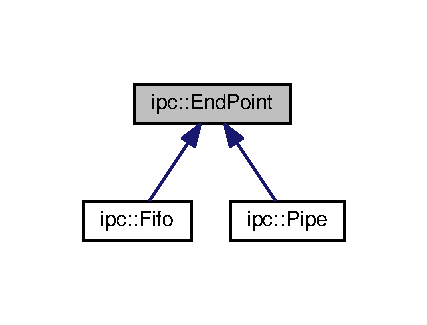
\includegraphics[width=205pt]{classipc_1_1EndPoint__inherit__graph}
\end{center}
\end{figure}


Collaboration diagram for ipc\+:\+:End\+Point\+:
\nopagebreak
\begin{figure}[H]
\begin{center}
\leavevmode
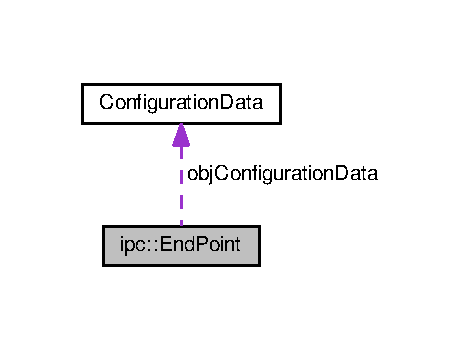
\includegraphics[width=222pt]{classipc_1_1EndPoint__coll__graph}
\end{center}
\end{figure}
\subsection*{Public Types}
\begin{DoxyCompactItemize}
\item 
enum \hyperlink{classipc_1_1EndPoint_adcdf30d3a61d3d342529b1fb8b0bbd72}{Protocol\+Type} \{ \hyperlink{classipc_1_1EndPoint_adcdf30d3a61d3d342529b1fb8b0bbd72a79ed024dca934b3dbe5150c824fa3f85}{T\+CP}, 
\hyperlink{classipc_1_1EndPoint_adcdf30d3a61d3d342529b1fb8b0bbd72a2e5b645e7fb05031f1c75d298db757b2}{U\+DP}
 \}
\item 
enum \hyperlink{classipc_1_1EndPoint_a5953c087a804e7c8c3e31fd97350b68a}{Socket\+Type} \{ \hyperlink{classipc_1_1EndPoint_a5953c087a804e7c8c3e31fd97350b68aaf20bc95cd10cd3a2dc9555f8affb9a75}{C\+L\+I\+E\+NT}, 
\hyperlink{classipc_1_1EndPoint_a5953c087a804e7c8c3e31fd97350b68aad92a281a0515f3dce327f63615417ae4}{S\+E\+R\+V\+ER}
 \}
\end{DoxyCompactItemize}
\subsection*{Public Member Functions}
\begin{DoxyCompactItemize}
\item 
virtual \hyperlink{classipc_1_1EndPoint_ad63e740860405b2073d51944accf3711}{$\sim$\+End\+Point} ()
\item 
virtual bool \hyperlink{classipc_1_1EndPoint_a11e6ea3b42eb264cd661abcd5c7398f4}{Initialize\+Log\+Mechanism} ()
\item 
virtual void \hyperlink{classipc_1_1EndPoint_a3a0ed19000bba31336d9e2d3f23e9e88}{initialize} (string str\+Name)=0
\item 
virtual Emp\+Full\+Message $\ast$ \hyperlink{classipc_1_1EndPoint_a6617ccd3bd8d8d314292db6ef3c9e7d5}{read\+Data} ()=0
\item 
virtual void \hyperlink{classipc_1_1EndPoint_a3dfd16e4b75e507f8c5fe9961934aa37}{write\+Data} (Emp\+Full\+Message $\ast$data)=0
\item 
virtual void \hyperlink{classipc_1_1EndPoint_a8d30be1048be238f4cef3240bfca143d}{destroy} ()=0
\item 
virtual bool \hyperlink{classipc_1_1EndPoint_a06f4cd9d1be23823c1f772da48779b58}{get\+Current\+State} ()=0
\end{DoxyCompactItemize}
\subsection*{Static Public Member Functions}
\begin{DoxyCompactItemize}
\item 
static void \hyperlink{classipc_1_1EndPoint_a22056e8bbdf6d8b1d901335acb7bdfba}{init\+Config\+Items} (string sz\+File\+Name)
\end{DoxyCompactItemize}
\subsection*{Static Public Attributes}
\begin{DoxyCompactItemize}
\item 
static \hyperlink{classConfigurationData}{Configuration\+Data} $\ast$ \hyperlink{classipc_1_1EndPoint_a7a04190956500a628f63f5d692ca6857}{obj\+Configuration\+Data} = N\+U\+LL
\end{DoxyCompactItemize}


\subsection{Detailed Description}


Definition at line 31 of file End\+Point.\+h.



\subsection{Member Enumeration Documentation}
\index{ipc\+::\+End\+Point@{ipc\+::\+End\+Point}!Protocol\+Type@{Protocol\+Type}}
\index{Protocol\+Type@{Protocol\+Type}!ipc\+::\+End\+Point@{ipc\+::\+End\+Point}}
\subsubsection[{\texorpdfstring{Protocol\+Type}{ProtocolType}}]{\setlength{\rightskip}{0pt plus 5cm}enum {\bf ipc\+::\+End\+Point\+::\+Protocol\+Type}}\hypertarget{classipc_1_1EndPoint_adcdf30d3a61d3d342529b1fb8b0bbd72}{}\label{classipc_1_1EndPoint_adcdf30d3a61d3d342529b1fb8b0bbd72}
\begin{Desc}
\item[Enumerator]\par
\begin{description}
\index{T\+CP@{T\+CP}!ipc\+::\+End\+Point@{ipc\+::\+End\+Point}}\index{ipc\+::\+End\+Point@{ipc\+::\+End\+Point}!T\+CP@{T\+CP}}\item[{\em 
T\+CP\hypertarget{classipc_1_1EndPoint_adcdf30d3a61d3d342529b1fb8b0bbd72a79ed024dca934b3dbe5150c824fa3f85}{}\label{classipc_1_1EndPoint_adcdf30d3a61d3d342529b1fb8b0bbd72a79ed024dca934b3dbe5150c824fa3f85}
}]\index{U\+DP@{U\+DP}!ipc\+::\+End\+Point@{ipc\+::\+End\+Point}}\index{ipc\+::\+End\+Point@{ipc\+::\+End\+Point}!U\+DP@{U\+DP}}\item[{\em 
U\+DP\hypertarget{classipc_1_1EndPoint_adcdf30d3a61d3d342529b1fb8b0bbd72a2e5b645e7fb05031f1c75d298db757b2}{}\label{classipc_1_1EndPoint_adcdf30d3a61d3d342529b1fb8b0bbd72a2e5b645e7fb05031f1c75d298db757b2}
}]\end{description}
\end{Desc}


Definition at line 36 of file End\+Point.\+h.

\index{ipc\+::\+End\+Point@{ipc\+::\+End\+Point}!Socket\+Type@{Socket\+Type}}
\index{Socket\+Type@{Socket\+Type}!ipc\+::\+End\+Point@{ipc\+::\+End\+Point}}
\subsubsection[{\texorpdfstring{Socket\+Type}{SocketType}}]{\setlength{\rightskip}{0pt plus 5cm}enum {\bf ipc\+::\+End\+Point\+::\+Socket\+Type}}\hypertarget{classipc_1_1EndPoint_a5953c087a804e7c8c3e31fd97350b68a}{}\label{classipc_1_1EndPoint_a5953c087a804e7c8c3e31fd97350b68a}
\begin{Desc}
\item[Enumerator]\par
\begin{description}
\index{C\+L\+I\+E\+NT@{C\+L\+I\+E\+NT}!ipc\+::\+End\+Point@{ipc\+::\+End\+Point}}\index{ipc\+::\+End\+Point@{ipc\+::\+End\+Point}!C\+L\+I\+E\+NT@{C\+L\+I\+E\+NT}}\item[{\em 
C\+L\+I\+E\+NT\hypertarget{classipc_1_1EndPoint_a5953c087a804e7c8c3e31fd97350b68aaf20bc95cd10cd3a2dc9555f8affb9a75}{}\label{classipc_1_1EndPoint_a5953c087a804e7c8c3e31fd97350b68aaf20bc95cd10cd3a2dc9555f8affb9a75}
}]\index{S\+E\+R\+V\+ER@{S\+E\+R\+V\+ER}!ipc\+::\+End\+Point@{ipc\+::\+End\+Point}}\index{ipc\+::\+End\+Point@{ipc\+::\+End\+Point}!S\+E\+R\+V\+ER@{S\+E\+R\+V\+ER}}\item[{\em 
S\+E\+R\+V\+ER\hypertarget{classipc_1_1EndPoint_a5953c087a804e7c8c3e31fd97350b68aad92a281a0515f3dce327f63615417ae4}{}\label{classipc_1_1EndPoint_a5953c087a804e7c8c3e31fd97350b68aad92a281a0515f3dce327f63615417ae4}
}]\end{description}
\end{Desc}


Definition at line 41 of file End\+Point.\+h.



\subsection{Constructor \& Destructor Documentation}
\index{ipc\+::\+End\+Point@{ipc\+::\+End\+Point}!````~End\+Point@{$\sim$\+End\+Point}}
\index{````~End\+Point@{$\sim$\+End\+Point}!ipc\+::\+End\+Point@{ipc\+::\+End\+Point}}
\subsubsection[{\texorpdfstring{$\sim$\+End\+Point()}{~EndPoint()}}]{\setlength{\rightskip}{0pt plus 5cm}End\+Point\+::$\sim$\+End\+Point (
\begin{DoxyParamCaption}
{}
\end{DoxyParamCaption}
)\hspace{0.3cm}{\ttfamily [virtual]}}\hypertarget{classipc_1_1EndPoint_ad63e740860405b2073d51944accf3711}{}\label{classipc_1_1EndPoint_ad63e740860405b2073d51944accf3711}


Definition at line 7 of file End\+Point.\+cpp.



\subsection{Member Function Documentation}
\index{ipc\+::\+End\+Point@{ipc\+::\+End\+Point}!destroy@{destroy}}
\index{destroy@{destroy}!ipc\+::\+End\+Point@{ipc\+::\+End\+Point}}
\subsubsection[{\texorpdfstring{destroy()=0}{destroy()=0}}]{\setlength{\rightskip}{0pt plus 5cm}virtual void ipc\+::\+End\+Point\+::destroy (
\begin{DoxyParamCaption}
{}
\end{DoxyParamCaption}
)\hspace{0.3cm}{\ttfamily [pure virtual]}}\hypertarget{classipc_1_1EndPoint_a8d30be1048be238f4cef3240bfca143d}{}\label{classipc_1_1EndPoint_a8d30be1048be238f4cef3240bfca143d}


Implemented in \hyperlink{classipc_1_1Pipe_a3f1de71c9add87611319d2838404dce3}{ipc\+::\+Pipe}, and \hyperlink{classipc_1_1Fifo_ac0797bc0cd5e0c2bf81aa4e1d6ed460f}{ipc\+::\+Fifo}.



Here is the caller graph for this function\+:
\nopagebreak
\begin{figure}[H]
\begin{center}
\leavevmode
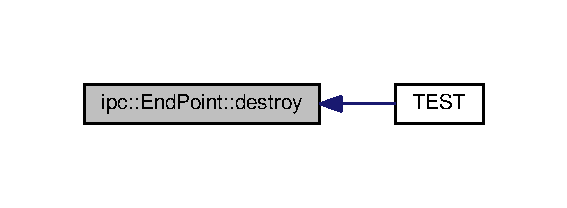
\includegraphics[width=272pt]{classipc_1_1EndPoint_a8d30be1048be238f4cef3240bfca143d_icgraph}
\end{center}
\end{figure}


\index{ipc\+::\+End\+Point@{ipc\+::\+End\+Point}!get\+Current\+State@{get\+Current\+State}}
\index{get\+Current\+State@{get\+Current\+State}!ipc\+::\+End\+Point@{ipc\+::\+End\+Point}}
\subsubsection[{\texorpdfstring{get\+Current\+State()=0}{getCurrentState()=0}}]{\setlength{\rightskip}{0pt plus 5cm}virtual bool ipc\+::\+End\+Point\+::get\+Current\+State (
\begin{DoxyParamCaption}
{}
\end{DoxyParamCaption}
)\hspace{0.3cm}{\ttfamily [pure virtual]}}\hypertarget{classipc_1_1EndPoint_a06f4cd9d1be23823c1f772da48779b58}{}\label{classipc_1_1EndPoint_a06f4cd9d1be23823c1f772da48779b58}


Implemented in \hyperlink{classipc_1_1Pipe_ab3c27bf2a9319b329f6fa380ec60d5f1}{ipc\+::\+Pipe}, and \hyperlink{classipc_1_1Fifo_aa409525e096829e18e1f9d8b07b49754}{ipc\+::\+Fifo}.

\index{ipc\+::\+End\+Point@{ipc\+::\+End\+Point}!init\+Config\+Items@{init\+Config\+Items}}
\index{init\+Config\+Items@{init\+Config\+Items}!ipc\+::\+End\+Point@{ipc\+::\+End\+Point}}
\subsubsection[{\texorpdfstring{init\+Config\+Items(string sz\+File\+Name)}{initConfigItems(string szFileName)}}]{\setlength{\rightskip}{0pt plus 5cm}void End\+Point\+::init\+Config\+Items (
\begin{DoxyParamCaption}
\item[{string}]{sz\+File\+Name}
\end{DoxyParamCaption}
)\hspace{0.3cm}{\ttfamily [static]}}\hypertarget{classipc_1_1EndPoint_a22056e8bbdf6d8b1d901335acb7bdfba}{}\label{classipc_1_1EndPoint_a22056e8bbdf6d8b1d901335acb7bdfba}


Definition at line 11 of file End\+Point.\+cpp.



Here is the caller graph for this function\+:
\nopagebreak
\begin{figure}[H]
\begin{center}
\leavevmode
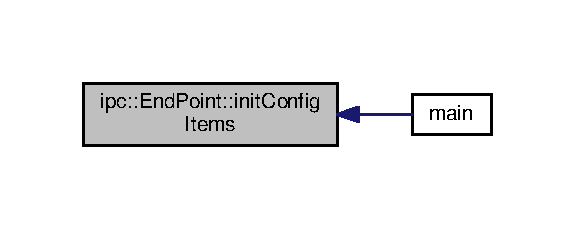
\includegraphics[width=276pt]{classipc_1_1EndPoint_a22056e8bbdf6d8b1d901335acb7bdfba_icgraph}
\end{center}
\end{figure}


\index{ipc\+::\+End\+Point@{ipc\+::\+End\+Point}!initialize@{initialize}}
\index{initialize@{initialize}!ipc\+::\+End\+Point@{ipc\+::\+End\+Point}}
\subsubsection[{\texorpdfstring{initialize(string str\+Name)=0}{initialize(string strName)=0}}]{\setlength{\rightskip}{0pt plus 5cm}virtual void ipc\+::\+End\+Point\+::initialize (
\begin{DoxyParamCaption}
\item[{string}]{str\+Name}
\end{DoxyParamCaption}
)\hspace{0.3cm}{\ttfamily [pure virtual]}}\hypertarget{classipc_1_1EndPoint_a3a0ed19000bba31336d9e2d3f23e9e88}{}\label{classipc_1_1EndPoint_a3a0ed19000bba31336d9e2d3f23e9e88}


Implemented in \hyperlink{classipc_1_1Pipe_adbae487d0da061626a372cf4b8dd9b39}{ipc\+::\+Pipe}, and \hyperlink{classipc_1_1Fifo_af8199c5aaa70ac42ea34f36a8209ecda}{ipc\+::\+Fifo}.



Here is the caller graph for this function\+:
\nopagebreak
\begin{figure}[H]
\begin{center}
\leavevmode
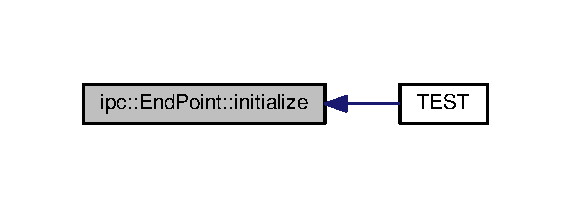
\includegraphics[width=274pt]{classipc_1_1EndPoint_a3a0ed19000bba31336d9e2d3f23e9e88_icgraph}
\end{center}
\end{figure}


\index{ipc\+::\+End\+Point@{ipc\+::\+End\+Point}!Initialize\+Log\+Mechanism@{Initialize\+Log\+Mechanism}}
\index{Initialize\+Log\+Mechanism@{Initialize\+Log\+Mechanism}!ipc\+::\+End\+Point@{ipc\+::\+End\+Point}}
\subsubsection[{\texorpdfstring{Initialize\+Log\+Mechanism()}{InitializeLogMechanism()}}]{\setlength{\rightskip}{0pt plus 5cm}bool End\+Point\+::\+Initialize\+Log\+Mechanism (
\begin{DoxyParamCaption}
{}
\end{DoxyParamCaption}
)\hspace{0.3cm}{\ttfamily [virtual]}}\hypertarget{classipc_1_1EndPoint_a11e6ea3b42eb264cd661abcd5c7398f4}{}\label{classipc_1_1EndPoint_a11e6ea3b42eb264cd661abcd5c7398f4}


Definition at line 24 of file End\+Point.\+cpp.

\index{ipc\+::\+End\+Point@{ipc\+::\+End\+Point}!read\+Data@{read\+Data}}
\index{read\+Data@{read\+Data}!ipc\+::\+End\+Point@{ipc\+::\+End\+Point}}
\subsubsection[{\texorpdfstring{read\+Data()=0}{readData()=0}}]{\setlength{\rightskip}{0pt plus 5cm}virtual Emp\+Full\+Message$\ast$ ipc\+::\+End\+Point\+::read\+Data (
\begin{DoxyParamCaption}
{}
\end{DoxyParamCaption}
)\hspace{0.3cm}{\ttfamily [pure virtual]}}\hypertarget{classipc_1_1EndPoint_a6617ccd3bd8d8d314292db6ef3c9e7d5}{}\label{classipc_1_1EndPoint_a6617ccd3bd8d8d314292db6ef3c9e7d5}


Implemented in \hyperlink{classipc_1_1Pipe_ac48948dba8e24c66d85c54594a813065}{ipc\+::\+Pipe}, and \hyperlink{classipc_1_1Fifo_a9c512a6ecabcc469432c068cdfeb7153}{ipc\+::\+Fifo}.



Here is the caller graph for this function\+:
\nopagebreak
\begin{figure}[H]
\begin{center}
\leavevmode
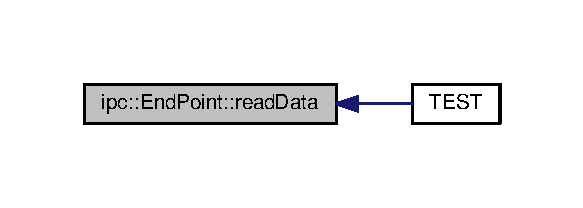
\includegraphics[width=280pt]{classipc_1_1EndPoint_a6617ccd3bd8d8d314292db6ef3c9e7d5_icgraph}
\end{center}
\end{figure}


\index{ipc\+::\+End\+Point@{ipc\+::\+End\+Point}!write\+Data@{write\+Data}}
\index{write\+Data@{write\+Data}!ipc\+::\+End\+Point@{ipc\+::\+End\+Point}}
\subsubsection[{\texorpdfstring{write\+Data(\+Emp\+Full\+Message $\ast$data)=0}{writeData(EmpFullMessage *data)=0}}]{\setlength{\rightskip}{0pt plus 5cm}virtual void ipc\+::\+End\+Point\+::write\+Data (
\begin{DoxyParamCaption}
\item[{Emp\+Full\+Message $\ast$}]{data}
\end{DoxyParamCaption}
)\hspace{0.3cm}{\ttfamily [pure virtual]}}\hypertarget{classipc_1_1EndPoint_a3dfd16e4b75e507f8c5fe9961934aa37}{}\label{classipc_1_1EndPoint_a3dfd16e4b75e507f8c5fe9961934aa37}


Implemented in \hyperlink{classipc_1_1Pipe_aa9d1114a883aef079d9f0d8d11fdd377}{ipc\+::\+Pipe}, and \hyperlink{classipc_1_1Fifo_aa134421064d4837dbd2361174fad955f}{ipc\+::\+Fifo}.



Here is the caller graph for this function\+:
\nopagebreak
\begin{figure}[H]
\begin{center}
\leavevmode
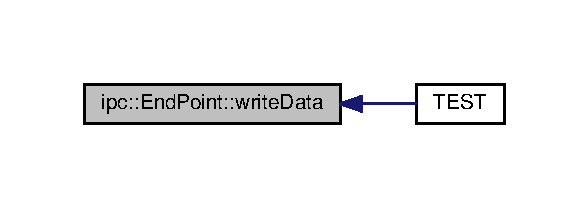
\includegraphics[width=282pt]{classipc_1_1EndPoint_a3dfd16e4b75e507f8c5fe9961934aa37_icgraph}
\end{center}
\end{figure}




\subsection{Member Data Documentation}
\index{ipc\+::\+End\+Point@{ipc\+::\+End\+Point}!obj\+Configuration\+Data@{obj\+Configuration\+Data}}
\index{obj\+Configuration\+Data@{obj\+Configuration\+Data}!ipc\+::\+End\+Point@{ipc\+::\+End\+Point}}
\subsubsection[{\texorpdfstring{obj\+Configuration\+Data}{objConfigurationData}}]{\setlength{\rightskip}{0pt plus 5cm}{\bf Configuration\+Data} $\ast$ End\+Point\+::obj\+Configuration\+Data = N\+U\+LL\hspace{0.3cm}{\ttfamily [static]}}\hypertarget{classipc_1_1EndPoint_a7a04190956500a628f63f5d692ca6857}{}\label{classipc_1_1EndPoint_a7a04190956500a628f63f5d692ca6857}


Definition at line 68 of file End\+Point.\+h.



The documentation for this class was generated from the following files\+:\begin{DoxyCompactItemize}
\item 
C\+O\+M\+M\+O\+N/\hyperlink{EndPoint_8h}{End\+Point.\+h}\item 
C\+O\+M\+M\+O\+N/\hyperlink{EndPoint_8cpp}{End\+Point.\+cpp}\end{DoxyCompactItemize}

\hypertarget{classipc_1_1EndPointFactory}{}\section{ipc\+:\+:End\+Point\+Factory Class Reference}
\label{classipc_1_1EndPointFactory}\index{ipc\+::\+End\+Point\+Factory@{ipc\+::\+End\+Point\+Factory}}


{\ttfamily \#include $<$End\+Point\+Factory.\+h$>$}

\subsection*{Public Types}
\begin{DoxyCompactItemize}
\item 
enum \hyperlink{classipc_1_1EndPointFactory_a436d6caf00a27aa28ca00bf116edca04}{End\+Point\+Type} \{ \\*
\hyperlink{classipc_1_1EndPointFactory_a436d6caf00a27aa28ca00bf116edca04ab4f2febf223e7103da442bcfe346789e}{I\+P\+C\+\_\+\+P\+I\+PE}, 
\hyperlink{classipc_1_1EndPointFactory_a436d6caf00a27aa28ca00bf116edca04aed25e2f8890e6f5c9a8b9b7215e378c0}{I\+P\+C\+\_\+\+F\+I\+FO}, 
\hyperlink{classipc_1_1EndPointFactory_a436d6caf00a27aa28ca00bf116edca04a8fa11a5e2ed1da22c16c97c530938cfa}{I\+P\+C\+\_\+\+SM}, 
\hyperlink{classipc_1_1EndPointFactory_a436d6caf00a27aa28ca00bf116edca04a07dfcba7770e093e86cb7e5fb5152827}{I\+P\+C\+\_\+\+MQ}, 
\\*
\hyperlink{classipc_1_1EndPointFactory_a436d6caf00a27aa28ca00bf116edca04a1e79496cd773f3410e261313944bf341}{I\+P\+C\+\_\+\+FL}, 
\hyperlink{classipc_1_1EndPointFactory_a436d6caf00a27aa28ca00bf116edca04af75cb0d4978f6067d53e887816c54c1c}{T\+C\+P\+\_\+\+IP}, 
\hyperlink{classipc_1_1EndPointFactory_a436d6caf00a27aa28ca00bf116edca04a53908264697bf3f606c27b77728dc80d}{I\+P\+C\+\_\+\+U\+DS}, 
\hyperlink{classipc_1_1EndPointFactory_a436d6caf00a27aa28ca00bf116edca04a4aef5054db3eecc660ec639e68b1346d}{E\+M\+P\+\_\+\+C\+L\+A\+S\+SD}
 \}
\end{DoxyCompactItemize}
\subsection*{Public Member Functions}
\begin{DoxyCompactItemize}
\item 
\hyperlink{classipc_1_1EndPoint}{End\+Point} $\ast$ \hyperlink{classipc_1_1EndPointFactory_a033e956410419b063d5074f4cd541048}{create\+End\+Point\+Instance} (\hyperlink{classipc_1_1EndPointFactory_a436d6caf00a27aa28ca00bf116edca04}{End\+Point\+Factory\+::\+End\+Point\+Type} end\+Point\+Type)
\item 
\hyperlink{classipc_1_1SocketEndPoint}{Socket\+End\+Point} $\ast$ \hyperlink{classipc_1_1EndPointFactory_a88cee65bcd3d20262fc289e0c61c1b2e}{create\+Socket\+End\+Point\+Instance} (\hyperlink{classipc_1_1EndPointFactory_a436d6caf00a27aa28ca00bf116edca04}{End\+Point\+Factory\+::\+End\+Point\+Type} end\+Point\+Type, \hyperlink{classipc_1_1EndPoint_adcdf30d3a61d3d342529b1fb8b0bbd72}{End\+Point\+::\+Protocol\+Type} protocol\+Type)
\end{DoxyCompactItemize}
\subsection*{Static Public Member Functions}
\begin{DoxyCompactItemize}
\item 
static \hyperlink{classipc_1_1EndPointFactory}{End\+Point\+Factory} $\ast$ \hyperlink{classipc_1_1EndPointFactory_a73f3fb990f682beeff892b65cf91a35b}{get\+End\+Point\+Factory} ()
\end{DoxyCompactItemize}


\subsection{Detailed Description}


Definition at line 12 of file End\+Point\+Factory.\+h.



\subsection{Member Enumeration Documentation}
\index{ipc\+::\+End\+Point\+Factory@{ipc\+::\+End\+Point\+Factory}!End\+Point\+Type@{End\+Point\+Type}}
\index{End\+Point\+Type@{End\+Point\+Type}!ipc\+::\+End\+Point\+Factory@{ipc\+::\+End\+Point\+Factory}}
\subsubsection[{\texorpdfstring{End\+Point\+Type}{EndPointType}}]{\setlength{\rightskip}{0pt plus 5cm}enum {\bf ipc\+::\+End\+Point\+Factory\+::\+End\+Point\+Type}}\hypertarget{classipc_1_1EndPointFactory_a436d6caf00a27aa28ca00bf116edca04}{}\label{classipc_1_1EndPointFactory_a436d6caf00a27aa28ca00bf116edca04}
\begin{Desc}
\item[Enumerator]\par
\begin{description}
\index{I\+P\+C\+\_\+\+P\+I\+PE@{I\+P\+C\+\_\+\+P\+I\+PE}!ipc\+::\+End\+Point\+Factory@{ipc\+::\+End\+Point\+Factory}}\index{ipc\+::\+End\+Point\+Factory@{ipc\+::\+End\+Point\+Factory}!I\+P\+C\+\_\+\+P\+I\+PE@{I\+P\+C\+\_\+\+P\+I\+PE}}\item[{\em 
I\+P\+C\+\_\+\+P\+I\+PE\hypertarget{classipc_1_1EndPointFactory_a436d6caf00a27aa28ca00bf116edca04ab4f2febf223e7103da442bcfe346789e}{}\label{classipc_1_1EndPointFactory_a436d6caf00a27aa28ca00bf116edca04ab4f2febf223e7103da442bcfe346789e}
}]\index{I\+P\+C\+\_\+\+F\+I\+FO@{I\+P\+C\+\_\+\+F\+I\+FO}!ipc\+::\+End\+Point\+Factory@{ipc\+::\+End\+Point\+Factory}}\index{ipc\+::\+End\+Point\+Factory@{ipc\+::\+End\+Point\+Factory}!I\+P\+C\+\_\+\+F\+I\+FO@{I\+P\+C\+\_\+\+F\+I\+FO}}\item[{\em 
I\+P\+C\+\_\+\+F\+I\+FO\hypertarget{classipc_1_1EndPointFactory_a436d6caf00a27aa28ca00bf116edca04aed25e2f8890e6f5c9a8b9b7215e378c0}{}\label{classipc_1_1EndPointFactory_a436d6caf00a27aa28ca00bf116edca04aed25e2f8890e6f5c9a8b9b7215e378c0}
}]\index{I\+P\+C\+\_\+\+SM@{I\+P\+C\+\_\+\+SM}!ipc\+::\+End\+Point\+Factory@{ipc\+::\+End\+Point\+Factory}}\index{ipc\+::\+End\+Point\+Factory@{ipc\+::\+End\+Point\+Factory}!I\+P\+C\+\_\+\+SM@{I\+P\+C\+\_\+\+SM}}\item[{\em 
I\+P\+C\+\_\+\+SM\hypertarget{classipc_1_1EndPointFactory_a436d6caf00a27aa28ca00bf116edca04a8fa11a5e2ed1da22c16c97c530938cfa}{}\label{classipc_1_1EndPointFactory_a436d6caf00a27aa28ca00bf116edca04a8fa11a5e2ed1da22c16c97c530938cfa}
}]\index{I\+P\+C\+\_\+\+MQ@{I\+P\+C\+\_\+\+MQ}!ipc\+::\+End\+Point\+Factory@{ipc\+::\+End\+Point\+Factory}}\index{ipc\+::\+End\+Point\+Factory@{ipc\+::\+End\+Point\+Factory}!I\+P\+C\+\_\+\+MQ@{I\+P\+C\+\_\+\+MQ}}\item[{\em 
I\+P\+C\+\_\+\+MQ\hypertarget{classipc_1_1EndPointFactory_a436d6caf00a27aa28ca00bf116edca04a07dfcba7770e093e86cb7e5fb5152827}{}\label{classipc_1_1EndPointFactory_a436d6caf00a27aa28ca00bf116edca04a07dfcba7770e093e86cb7e5fb5152827}
}]\index{I\+P\+C\+\_\+\+FL@{I\+P\+C\+\_\+\+FL}!ipc\+::\+End\+Point\+Factory@{ipc\+::\+End\+Point\+Factory}}\index{ipc\+::\+End\+Point\+Factory@{ipc\+::\+End\+Point\+Factory}!I\+P\+C\+\_\+\+FL@{I\+P\+C\+\_\+\+FL}}\item[{\em 
I\+P\+C\+\_\+\+FL\hypertarget{classipc_1_1EndPointFactory_a436d6caf00a27aa28ca00bf116edca04a1e79496cd773f3410e261313944bf341}{}\label{classipc_1_1EndPointFactory_a436d6caf00a27aa28ca00bf116edca04a1e79496cd773f3410e261313944bf341}
}]\index{T\+C\+P\+\_\+\+IP@{T\+C\+P\+\_\+\+IP}!ipc\+::\+End\+Point\+Factory@{ipc\+::\+End\+Point\+Factory}}\index{ipc\+::\+End\+Point\+Factory@{ipc\+::\+End\+Point\+Factory}!T\+C\+P\+\_\+\+IP@{T\+C\+P\+\_\+\+IP}}\item[{\em 
T\+C\+P\+\_\+\+IP\hypertarget{classipc_1_1EndPointFactory_a436d6caf00a27aa28ca00bf116edca04af75cb0d4978f6067d53e887816c54c1c}{}\label{classipc_1_1EndPointFactory_a436d6caf00a27aa28ca00bf116edca04af75cb0d4978f6067d53e887816c54c1c}
}]\index{I\+P\+C\+\_\+\+U\+DS@{I\+P\+C\+\_\+\+U\+DS}!ipc\+::\+End\+Point\+Factory@{ipc\+::\+End\+Point\+Factory}}\index{ipc\+::\+End\+Point\+Factory@{ipc\+::\+End\+Point\+Factory}!I\+P\+C\+\_\+\+U\+DS@{I\+P\+C\+\_\+\+U\+DS}}\item[{\em 
I\+P\+C\+\_\+\+U\+DS\hypertarget{classipc_1_1EndPointFactory_a436d6caf00a27aa28ca00bf116edca04a53908264697bf3f606c27b77728dc80d}{}\label{classipc_1_1EndPointFactory_a436d6caf00a27aa28ca00bf116edca04a53908264697bf3f606c27b77728dc80d}
}]\index{E\+M\+P\+\_\+\+C\+L\+A\+S\+SD@{E\+M\+P\+\_\+\+C\+L\+A\+S\+SD}!ipc\+::\+End\+Point\+Factory@{ipc\+::\+End\+Point\+Factory}}\index{ipc\+::\+End\+Point\+Factory@{ipc\+::\+End\+Point\+Factory}!E\+M\+P\+\_\+\+C\+L\+A\+S\+SD@{E\+M\+P\+\_\+\+C\+L\+A\+S\+SD}}\item[{\em 
E\+M\+P\+\_\+\+C\+L\+A\+S\+SD\hypertarget{classipc_1_1EndPointFactory_a436d6caf00a27aa28ca00bf116edca04a4aef5054db3eecc660ec639e68b1346d}{}\label{classipc_1_1EndPointFactory_a436d6caf00a27aa28ca00bf116edca04a4aef5054db3eecc660ec639e68b1346d}
}]\end{description}
\end{Desc}


Definition at line 21 of file End\+Point\+Factory.\+h.



\subsection{Member Function Documentation}
\index{ipc\+::\+End\+Point\+Factory@{ipc\+::\+End\+Point\+Factory}!create\+End\+Point\+Instance@{create\+End\+Point\+Instance}}
\index{create\+End\+Point\+Instance@{create\+End\+Point\+Instance}!ipc\+::\+End\+Point\+Factory@{ipc\+::\+End\+Point\+Factory}}
\subsubsection[{\texorpdfstring{create\+End\+Point\+Instance(\+End\+Point\+Factory\+::\+End\+Point\+Type end\+Point\+Type)}{createEndPointInstance(EndPointFactory::EndPointType endPointType)}}]{\setlength{\rightskip}{0pt plus 5cm}{\bf End\+Point} $\ast$ End\+Point\+Factory\+::create\+End\+Point\+Instance (
\begin{DoxyParamCaption}
\item[{{\bf End\+Point\+Factory\+::\+End\+Point\+Type}}]{end\+Point\+Type}
\end{DoxyParamCaption}
)}\hypertarget{classipc_1_1EndPointFactory_a033e956410419b063d5074f4cd541048}{}\label{classipc_1_1EndPointFactory_a033e956410419b063d5074f4cd541048}


Definition at line 32 of file End\+Point\+Factory.\+cpp.



Here is the caller graph for this function\+:
\nopagebreak
\begin{figure}[H]
\begin{center}
\leavevmode
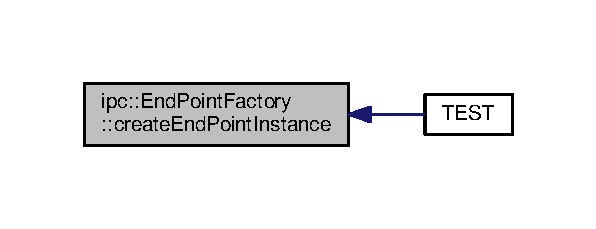
\includegraphics[width=286pt]{classipc_1_1EndPointFactory_a033e956410419b063d5074f4cd541048_icgraph}
\end{center}
\end{figure}


\index{ipc\+::\+End\+Point\+Factory@{ipc\+::\+End\+Point\+Factory}!create\+Socket\+End\+Point\+Instance@{create\+Socket\+End\+Point\+Instance}}
\index{create\+Socket\+End\+Point\+Instance@{create\+Socket\+End\+Point\+Instance}!ipc\+::\+End\+Point\+Factory@{ipc\+::\+End\+Point\+Factory}}
\subsubsection[{\texorpdfstring{create\+Socket\+End\+Point\+Instance(\+End\+Point\+Factory\+::\+End\+Point\+Type end\+Point\+Type, End\+Point\+::\+Protocol\+Type protocol\+Type)}{createSocketEndPointInstance(EndPointFactory::EndPointType endPointType, EndPoint::ProtocolType protocolType)}}]{\setlength{\rightskip}{0pt plus 5cm}{\bf Socket\+End\+Point} $\ast$ End\+Point\+Factory\+::create\+Socket\+End\+Point\+Instance (
\begin{DoxyParamCaption}
\item[{{\bf End\+Point\+Factory\+::\+End\+Point\+Type}}]{end\+Point\+Type, }
\item[{{\bf End\+Point\+::\+Protocol\+Type}}]{protocol\+Type}
\end{DoxyParamCaption}
)}\hypertarget{classipc_1_1EndPointFactory_a88cee65bcd3d20262fc289e0c61c1b2e}{}\label{classipc_1_1EndPointFactory_a88cee65bcd3d20262fc289e0c61c1b2e}


Definition at line 62 of file End\+Point\+Factory.\+cpp.



Here is the caller graph for this function\+:
\nopagebreak
\begin{figure}[H]
\begin{center}
\leavevmode
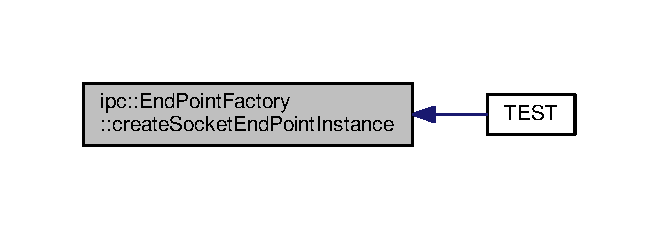
\includegraphics[width=316pt]{classipc_1_1EndPointFactory_a88cee65bcd3d20262fc289e0c61c1b2e_icgraph}
\end{center}
\end{figure}


\index{ipc\+::\+End\+Point\+Factory@{ipc\+::\+End\+Point\+Factory}!get\+End\+Point\+Factory@{get\+End\+Point\+Factory}}
\index{get\+End\+Point\+Factory@{get\+End\+Point\+Factory}!ipc\+::\+End\+Point\+Factory@{ipc\+::\+End\+Point\+Factory}}
\subsubsection[{\texorpdfstring{get\+End\+Point\+Factory()}{getEndPointFactory()}}]{\setlength{\rightskip}{0pt plus 5cm}{\bf End\+Point\+Factory} $\ast$ End\+Point\+Factory\+::get\+End\+Point\+Factory (
\begin{DoxyParamCaption}
{}
\end{DoxyParamCaption}
)\hspace{0.3cm}{\ttfamily [static]}}\hypertarget{classipc_1_1EndPointFactory_a73f3fb990f682beeff892b65cf91a35b}{}\label{classipc_1_1EndPointFactory_a73f3fb990f682beeff892b65cf91a35b}


Definition at line 25 of file End\+Point\+Factory.\+cpp.



The documentation for this class was generated from the following files\+:\begin{DoxyCompactItemize}
\item 
C\+O\+M\+M\+O\+N/\hyperlink{EndPointFactory_8h}{End\+Point\+Factory.\+h}\item 
C\+O\+M\+M\+O\+N/\hyperlink{EndPointFactory_8cpp}{End\+Point\+Factory.\+cpp}\end{DoxyCompactItemize}

\hypertarget{classipc_1_1Fifo}{}\section{ipc\+:\+:Fifo Class Reference}
\label{classipc_1_1Fifo}\index{ipc\+::\+Fifo@{ipc\+::\+Fifo}}


{\ttfamily \#include $<$Fifo.\+h$>$}



Inheritance diagram for ipc\+:\+:Fifo\+:
\nopagebreak
\begin{figure}[H]
\begin{center}
\leavevmode
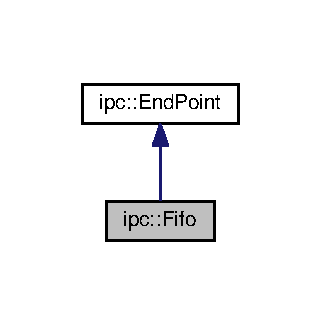
\includegraphics[width=154pt]{classipc_1_1Fifo__inherit__graph}
\end{center}
\end{figure}


Collaboration diagram for ipc\+:\+:Fifo\+:
\nopagebreak
\begin{figure}[H]
\begin{center}
\leavevmode
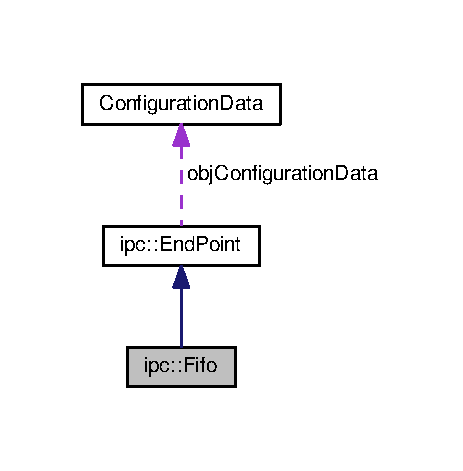
\includegraphics[width=222pt]{classipc_1_1Fifo__coll__graph}
\end{center}
\end{figure}
\subsection*{Public Member Functions}
\begin{DoxyCompactItemize}
\item 
\hyperlink{classipc_1_1Fifo_a5b466d3a17d14a6737a64e478b52ae3a}{Fifo} ()
\item 
virtual \hyperlink{classipc_1_1Fifo_ac057810a530bf36506bd87ecd0a52964}{$\sim$\+Fifo} ()
\item 
void \hyperlink{classipc_1_1Fifo_af8199c5aaa70ac42ea34f36a8209ecda}{initialize} (string str\+Name)
\item 
Emp\+Full\+Message $\ast$ \hyperlink{classipc_1_1Fifo_a9c512a6ecabcc469432c068cdfeb7153}{read\+Data} ()
\item 
void \hyperlink{classipc_1_1Fifo_aa134421064d4837dbd2361174fad955f}{write\+Data} (Emp\+Full\+Message $\ast$message)
\item 
void \hyperlink{classipc_1_1Fifo_ac0797bc0cd5e0c2bf81aa4e1d6ed460f}{destroy} ()
\item 
bool \hyperlink{classipc_1_1Fifo_aa409525e096829e18e1f9d8b07b49754}{get\+Current\+State} ()
\end{DoxyCompactItemize}
\subsection*{Additional Inherited Members}


\subsection{Detailed Description}


Definition at line 17 of file Fifo.\+h.



\subsection{Constructor \& Destructor Documentation}
\index{ipc\+::\+Fifo@{ipc\+::\+Fifo}!Fifo@{Fifo}}
\index{Fifo@{Fifo}!ipc\+::\+Fifo@{ipc\+::\+Fifo}}
\subsubsection[{\texorpdfstring{Fifo()}{Fifo()}}]{\setlength{\rightskip}{0pt plus 5cm}Fifo\+::\+Fifo (
\begin{DoxyParamCaption}
{}
\end{DoxyParamCaption}
)}\hypertarget{classipc_1_1Fifo_a5b466d3a17d14a6737a64e478b52ae3a}{}\label{classipc_1_1Fifo_a5b466d3a17d14a6737a64e478b52ae3a}


Definition at line 24 of file Fifo.\+cpp.

\index{ipc\+::\+Fifo@{ipc\+::\+Fifo}!````~Fifo@{$\sim$\+Fifo}}
\index{````~Fifo@{$\sim$\+Fifo}!ipc\+::\+Fifo@{ipc\+::\+Fifo}}
\subsubsection[{\texorpdfstring{$\sim$\+Fifo()}{~Fifo()}}]{\setlength{\rightskip}{0pt plus 5cm}Fifo\+::$\sim$\+Fifo (
\begin{DoxyParamCaption}
{}
\end{DoxyParamCaption}
)\hspace{0.3cm}{\ttfamily [virtual]}}\hypertarget{classipc_1_1Fifo_ac057810a530bf36506bd87ecd0a52964}{}\label{classipc_1_1Fifo_ac057810a530bf36506bd87ecd0a52964}


Definition at line 33 of file Fifo.\+cpp.



\subsection{Member Function Documentation}
\index{ipc\+::\+Fifo@{ipc\+::\+Fifo}!destroy@{destroy}}
\index{destroy@{destroy}!ipc\+::\+Fifo@{ipc\+::\+Fifo}}
\subsubsection[{\texorpdfstring{destroy()}{destroy()}}]{\setlength{\rightskip}{0pt plus 5cm}void Fifo\+::destroy (
\begin{DoxyParamCaption}
{}
\end{DoxyParamCaption}
)\hspace{0.3cm}{\ttfamily [virtual]}}\hypertarget{classipc_1_1Fifo_ac0797bc0cd5e0c2bf81aa4e1d6ed460f}{}\label{classipc_1_1Fifo_ac0797bc0cd5e0c2bf81aa4e1d6ed460f}


Implements \hyperlink{classipc_1_1EndPoint_a8d30be1048be238f4cef3240bfca143d}{ipc\+::\+End\+Point}.



Definition at line 180 of file Fifo.\+cpp.

\index{ipc\+::\+Fifo@{ipc\+::\+Fifo}!get\+Current\+State@{get\+Current\+State}}
\index{get\+Current\+State@{get\+Current\+State}!ipc\+::\+Fifo@{ipc\+::\+Fifo}}
\subsubsection[{\texorpdfstring{get\+Current\+State()}{getCurrentState()}}]{\setlength{\rightskip}{0pt plus 5cm}bool Fifo\+::get\+Current\+State (
\begin{DoxyParamCaption}
{}
\end{DoxyParamCaption}
)\hspace{0.3cm}{\ttfamily [virtual]}}\hypertarget{classipc_1_1Fifo_aa409525e096829e18e1f9d8b07b49754}{}\label{classipc_1_1Fifo_aa409525e096829e18e1f9d8b07b49754}


Implements \hyperlink{classipc_1_1EndPoint_a06f4cd9d1be23823c1f772da48779b58}{ipc\+::\+End\+Point}.



Definition at line 191 of file Fifo.\+cpp.

\index{ipc\+::\+Fifo@{ipc\+::\+Fifo}!initialize@{initialize}}
\index{initialize@{initialize}!ipc\+::\+Fifo@{ipc\+::\+Fifo}}
\subsubsection[{\texorpdfstring{initialize(string str\+Name)}{initialize(string strName)}}]{\setlength{\rightskip}{0pt plus 5cm}void Fifo\+::initialize (
\begin{DoxyParamCaption}
\item[{string}]{str\+Name}
\end{DoxyParamCaption}
)\hspace{0.3cm}{\ttfamily [virtual]}}\hypertarget{classipc_1_1Fifo_af8199c5aaa70ac42ea34f36a8209ecda}{}\label{classipc_1_1Fifo_af8199c5aaa70ac42ea34f36a8209ecda}


Implements \hyperlink{classipc_1_1EndPoint_a3a0ed19000bba31336d9e2d3f23e9e88}{ipc\+::\+End\+Point}.



Definition at line 43 of file Fifo.\+cpp.

\index{ipc\+::\+Fifo@{ipc\+::\+Fifo}!read\+Data@{read\+Data}}
\index{read\+Data@{read\+Data}!ipc\+::\+Fifo@{ipc\+::\+Fifo}}
\subsubsection[{\texorpdfstring{read\+Data()}{readData()}}]{\setlength{\rightskip}{0pt plus 5cm}Emp\+Full\+Message $\ast$ Fifo\+::read\+Data (
\begin{DoxyParamCaption}
{}
\end{DoxyParamCaption}
)\hspace{0.3cm}{\ttfamily [virtual]}}\hypertarget{classipc_1_1Fifo_a9c512a6ecabcc469432c068cdfeb7153}{}\label{classipc_1_1Fifo_a9c512a6ecabcc469432c068cdfeb7153}


Implements \hyperlink{classipc_1_1EndPoint_a6617ccd3bd8d8d314292db6ef3c9e7d5}{ipc\+::\+End\+Point}.



Definition at line 84 of file Fifo.\+cpp.

\index{ipc\+::\+Fifo@{ipc\+::\+Fifo}!write\+Data@{write\+Data}}
\index{write\+Data@{write\+Data}!ipc\+::\+Fifo@{ipc\+::\+Fifo}}
\subsubsection[{\texorpdfstring{write\+Data(\+Emp\+Full\+Message $\ast$message)}{writeData(EmpFullMessage *message)}}]{\setlength{\rightskip}{0pt plus 5cm}void Fifo\+::write\+Data (
\begin{DoxyParamCaption}
\item[{Emp\+Full\+Message $\ast$}]{message}
\end{DoxyParamCaption}
)\hspace{0.3cm}{\ttfamily [virtual]}}\hypertarget{classipc_1_1Fifo_aa134421064d4837dbd2361174fad955f}{}\label{classipc_1_1Fifo_aa134421064d4837dbd2361174fad955f}


Implements \hyperlink{classipc_1_1EndPoint_a3dfd16e4b75e507f8c5fe9961934aa37}{ipc\+::\+End\+Point}.



Definition at line 150 of file Fifo.\+cpp.



The documentation for this class was generated from the following files\+:\begin{DoxyCompactItemize}
\item 
I\+P\+C\+\_\+\+F\+I\+F\+O/\hyperlink{Fifo_8h}{Fifo.\+h}\item 
I\+P\+C\+\_\+\+F\+I\+F\+O/\hyperlink{Fifo_8cpp}{Fifo.\+cpp}\end{DoxyCompactItemize}

\hypertarget{classFileBasedConfiguration}{}\section{File\+Based\+Configuration Class Reference}
\label{classFileBasedConfiguration}\index{File\+Based\+Configuration@{File\+Based\+Configuration}}


{\ttfamily \#include $<$File\+Based\+Configuration.\+h$>$}

\subsection*{Public Member Functions}
\begin{DoxyCompactItemize}
\item 
\hyperlink{classFileBasedConfiguration_a83577180aecfeafb83e68437e8c7bd7d}{File\+Based\+Configuration} ()
\item 
virtual \hyperlink{classFileBasedConfiguration_a7d187cd831e37c33e6d1d202e57c0ecf}{$\sim$\+File\+Based\+Configuration} ()
\item 
map$<$ string, vector$<$ \hyperlink{structDynamicConfigItemDataStruct}{Dynamic\+Config\+Item\+Data\+Struct} $>$ $>$ \hyperlink{classFileBasedConfiguration_af0ac0445ddef7bdf5de10f5a0b7b07e1}{parse\+The\+Configuration\+Xml} (string file\+Name, bool \&is\+Success)
\end{DoxyCompactItemize}


\subsection{Detailed Description}


Definition at line 20 of file File\+Based\+Configuration.\+h.



\subsection{Constructor \& Destructor Documentation}
\index{File\+Based\+Configuration@{File\+Based\+Configuration}!File\+Based\+Configuration@{File\+Based\+Configuration}}
\index{File\+Based\+Configuration@{File\+Based\+Configuration}!File\+Based\+Configuration@{File\+Based\+Configuration}}
\subsubsection[{\texorpdfstring{File\+Based\+Configuration()}{FileBasedConfiguration()}}]{\setlength{\rightskip}{0pt plus 5cm}File\+Based\+Configuration\+::\+File\+Based\+Configuration (
\begin{DoxyParamCaption}
{}
\end{DoxyParamCaption}
)}\hypertarget{classFileBasedConfiguration_a83577180aecfeafb83e68437e8c7bd7d}{}\label{classFileBasedConfiguration_a83577180aecfeafb83e68437e8c7bd7d}
\index{File\+Based\+Configuration@{File\+Based\+Configuration}!````~File\+Based\+Configuration@{$\sim$\+File\+Based\+Configuration}}
\index{````~File\+Based\+Configuration@{$\sim$\+File\+Based\+Configuration}!File\+Based\+Configuration@{File\+Based\+Configuration}}
\subsubsection[{\texorpdfstring{$\sim$\+File\+Based\+Configuration()}{~FileBasedConfiguration()}}]{\setlength{\rightskip}{0pt plus 5cm}virtual File\+Based\+Configuration\+::$\sim$\+File\+Based\+Configuration (
\begin{DoxyParamCaption}
{}
\end{DoxyParamCaption}
)\hspace{0.3cm}{\ttfamily [virtual]}}\hypertarget{classFileBasedConfiguration_a7d187cd831e37c33e6d1d202e57c0ecf}{}\label{classFileBasedConfiguration_a7d187cd831e37c33e6d1d202e57c0ecf}


\subsection{Member Function Documentation}
\index{File\+Based\+Configuration@{File\+Based\+Configuration}!parse\+The\+Configuration\+Xml@{parse\+The\+Configuration\+Xml}}
\index{parse\+The\+Configuration\+Xml@{parse\+The\+Configuration\+Xml}!File\+Based\+Configuration@{File\+Based\+Configuration}}
\subsubsection[{\texorpdfstring{parse\+The\+Configuration\+Xml(string file\+Name, bool \&is\+Success)}{parseTheConfigurationXml(string fileName, bool &isSuccess)}}]{\setlength{\rightskip}{0pt plus 5cm}map$<$string, vector $<${\bf Dynamic\+Config\+Item\+Data\+Struct}$>$ $>$ File\+Based\+Configuration\+::parse\+The\+Configuration\+Xml (
\begin{DoxyParamCaption}
\item[{string}]{file\+Name, }
\item[{bool \&}]{is\+Success}
\end{DoxyParamCaption}
)}\hypertarget{classFileBasedConfiguration_af0ac0445ddef7bdf5de10f5a0b7b07e1}{}\label{classFileBasedConfiguration_af0ac0445ddef7bdf5de10f5a0b7b07e1}


The documentation for this class was generated from the following file\+:\begin{DoxyCompactItemize}
\item 
D\+Y\+N\+\_\+\+C\+O\+N\+F\+I\+G/include/\hyperlink{FileBasedConfiguration_8h}{File\+Based\+Configuration.\+h}\end{DoxyCompactItemize}

\hypertarget{classutils_1_1Log}{}\section{utils\+:\+:Log Class Reference}
\label{classutils_1_1Log}\index{utils\+::\+Log@{utils\+::\+Log}}


{\ttfamily \#include $<$Log.\+h$>$}

\subsection*{Public Types}
\begin{DoxyCompactItemize}
\item 
enum \hyperlink{classutils_1_1Log_a8f981afda2b7802a6e9ca4aac269d54a}{Log\+Levels} \{ \\*
\hyperlink{classutils_1_1Log_a8f981afda2b7802a6e9ca4aac269d54aaa3a7218440adf6d603dcaceabb683a12}{E\+R\+R\+O\+R\+\_\+\+L\+E\+V\+EL} = 1, 
\hyperlink{classutils_1_1Log_a8f981afda2b7802a6e9ca4aac269d54aac494c60808c9ca13881edb977d888127}{W\+A\+R\+N\+\_\+\+L\+E\+V\+EL} = 2, 
\hyperlink{classutils_1_1Log_a8f981afda2b7802a6e9ca4aac269d54aa9c80ebf03876dd47244938a0d60631a5}{I\+N\+F\+O\+\_\+\+L\+E\+V\+EL} = 3, 
\hyperlink{classutils_1_1Log_a8f981afda2b7802a6e9ca4aac269d54aa023731e6ba36eed6733acfa4e182dc85}{T\+R\+A\+C\+E\+\_\+\+L\+E\+V\+EL} = 4, 
\\*
\hyperlink{classutils_1_1Log_a8f981afda2b7802a6e9ca4aac269d54aab0e7af85fa3d909da693e83b540ac2a3}{E\+N\+D\+\_\+\+O\+F\+\_\+\+Log\+Levels}
 \}
\item 
enum \hyperlink{classutils_1_1Log_aeb031aea7d8d59f98a6857915d32e864}{Elaps\+Tm\+Lvls} \{ \\*
\hyperlink{classutils_1_1Log_aeb031aea7d8d59f98a6857915d32e864ac2b82d02aa2ddf29cc1e3f5385644267}{E\+L\+A\+P\+S\+T\+M\+\_\+\+S\+U\+M\+M\+A\+RY} = 1, 
\hyperlink{classutils_1_1Log_aeb031aea7d8d59f98a6857915d32e864a14889f3c1fee759c05748d57ffe33798}{E\+L\+A\+P\+S\+T\+M\+\_\+\+D\+E\+T\+A\+I\+L\+ED} = 2, 
\hyperlink{classutils_1_1Log_aeb031aea7d8d59f98a6857915d32e864a35b8d83c7001e838bdab3500441becd8}{E\+L\+A\+P\+S\+T\+M\+\_\+\+O\+U\+T\+\_\+\+O\+F\+\_\+\+R\+A\+N\+GE} = 4, 
\hyperlink{classutils_1_1Log_aeb031aea7d8d59f98a6857915d32e864ae1ccab5063c41d5d18e2cd7535a55983}{E\+L\+A\+P\+S\+T\+M\+\_\+\+D\+I\+S\+A\+B\+L\+ED} = 8, 
\\*
\hyperlink{classutils_1_1Log_aeb031aea7d8d59f98a6857915d32e864ad1c7a76ee5bd172473f5018c310d9eaa}{E\+N\+D\+\_\+\+O\+F\+\_\+\+Elaps\+Tm\+Lvls} = 16
 \}
\item 
enum \hyperlink{classutils_1_1Log_aa77064096777fe92d4ff8f6d68d42d5a}{Log\+Dest} \{ \\*
\hyperlink{classutils_1_1Log_aa77064096777fe92d4ff8f6d68d42d5aa073188971cc5f6222bcd080faba0e170}{N\+O\+NE} = 0, 
\hyperlink{classutils_1_1Log_aa77064096777fe92d4ff8f6d68d42d5aaa4c1e78fb35ae098bba52e43e2a5e0e5}{F\+I\+LE} = 1, 
\hyperlink{classutils_1_1Log_aa77064096777fe92d4ff8f6d68d42d5aa9b86815165af42d845410f10dfd2e061}{D\+A\+T\+A\+B\+A\+SE} = 2, 
\hyperlink{classutils_1_1Log_aa77064096777fe92d4ff8f6d68d42d5aa777a40d3f6fbce3f8d928c9d791e6d03}{B\+O\+TH} = 3, 
\\*
\hyperlink{classutils_1_1Log_aa77064096777fe92d4ff8f6d68d42d5aacabf499629d9834d891a51d030cdef68}{E\+N\+D\+\_\+\+O\+F\+\_\+\+Log\+Dest}
 \}
\end{DoxyCompactItemize}
\subsection*{Public Member Functions}
\begin{DoxyCompactItemize}
\item 
\hyperlink{classutils_1_1Log_a889fde15d21820f27d32315d53e75a06}{Log} ()
\item 
\hyperlink{classutils_1_1Log_aca4c4527042fc72294f36013924bb309}{$\sim$\+Log} ()
\end{DoxyCompactItemize}
\subsection*{Static Public Member Functions}
\begin{DoxyCompactItemize}
\item 
static bool \hyperlink{classutils_1_1Log_ad5b43b0f5ea6a8b447407a33cda5a4bf}{is\+Trace\+Enabled} ()
\item 
static bool \hyperlink{classutils_1_1Log_af831fb2def9d0984c712ca6c73cf2cd8}{is\+Info\+Enabled} ()
\item 
static bool \hyperlink{classutils_1_1Log_a99a23d525a51c3290f793dedadc65470}{is\+Warn\+Enabled} ()
\item 
static bool \hyperlink{classutils_1_1Log_ac8b80b98cd9f5de11e53980a873862a4}{is\+Error\+Enabled} ()
\item 
static void \hyperlink{classutils_1_1Log_a78fee29378f2064f9ee8299cb59d26ce}{init} (const char $\ast$value)
\begin{DoxyCompactList}\small\item\em Deprecated methods (Remove as soon as possible) /////. \end{DoxyCompactList}\item 
static void \hyperlink{classutils_1_1Log_a0a94150091c4d2768da2eac92006bdc7}{init} (const char $\ast$logapp, const char $\ast$logdir, const \hyperlink{classutils_1_1Log_a8f981afda2b7802a6e9ca4aac269d54a}{Log\+Levels} prio\+Lvl, const bool flag)
\item 
static void \hyperlink{classutils_1_1Log_aecbaeed2809b1cf54b5d78fbc9870ebe}{set\+Elapsed} (char $\ast$value, int mask)
\item 
static void \hyperlink{classutils_1_1Log_a37ae89eca0ad705c5e948710406e2054}{trace} (const char $\ast$sz\+File\+Name, const int n\+Line\+Number, const char $\ast$sz\+Msg, const char $\ast$sz\+Application\+Id=N\+U\+LL, const char $\ast$sz\+Method\+Name=N\+U\+LL, const char $\ast$sz\+Src\+Filename=N\+U\+LL, \hyperlink{classutils_1_1Log_aa77064096777fe92d4ff8f6d68d42d5a}{Log\+::\+Log\+Dest} nlog\+Dest=\hyperlink{classutils_1_1Log_aa77064096777fe92d4ff8f6d68d42d5aaa4c1e78fb35ae098bba52e43e2a5e0e5}{Log\+::\+F\+I\+LE}, bool use\+Param\+Destination=false)
\item 
static void \hyperlink{classutils_1_1Log_acee86547a863c04b349ab46a3b7ba9f2}{info} (const char $\ast$sz\+File\+Name, const int n\+Line\+Number, const char $\ast$sz\+Msg, const char $\ast$sz\+Application\+Id=N\+U\+LL, const char $\ast$sz\+Method\+Name=N\+U\+LL, const char $\ast$sz\+Src\+Filename=N\+U\+LL, \hyperlink{classutils_1_1Log_aa77064096777fe92d4ff8f6d68d42d5a}{Log\+::\+Log\+Dest} nlog\+Dest=\hyperlink{classutils_1_1Log_aa77064096777fe92d4ff8f6d68d42d5aaa4c1e78fb35ae098bba52e43e2a5e0e5}{Log\+::\+F\+I\+LE}, bool use\+Param\+Destination=false)
\item 
static void \hyperlink{classutils_1_1Log_aaff384f2d48d78b72b9c5e72ebed18db}{warn} (const char $\ast$sz\+File\+Name, const int n\+Line\+Number, const char $\ast$sz\+Msg, const char $\ast$sz\+Application\+Id=N\+U\+LL, const char $\ast$sz\+Method\+Name=N\+U\+LL, const char $\ast$sz\+Src\+Filename=N\+U\+LL, \hyperlink{classutils_1_1Log_aa77064096777fe92d4ff8f6d68d42d5a}{Log\+::\+Log\+Dest} nlog\+Dest=\hyperlink{classutils_1_1Log_aa77064096777fe92d4ff8f6d68d42d5aaa4c1e78fb35ae098bba52e43e2a5e0e5}{Log\+::\+F\+I\+LE}, bool use\+Param\+Destination=false)
\item 
static void \hyperlink{classutils_1_1Log_a79149fab5ab512aef26dbebc45e936d1}{error} (const char $\ast$sz\+File\+Name, const int n\+Line\+Number, const char $\ast$sz\+Msg, const char $\ast$sz\+Application\+Id=N\+U\+LL, const char $\ast$sz\+Method\+Name=N\+U\+LL, const char $\ast$sz\+Src\+Filename=N\+U\+LL, \hyperlink{classutils_1_1Log_aa77064096777fe92d4ff8f6d68d42d5a}{Log\+::\+Log\+Dest} nlog\+Dest=\hyperlink{classutils_1_1Log_aa77064096777fe92d4ff8f6d68d42d5aaa4c1e78fb35ae098bba52e43e2a5e0e5}{Log\+::\+F\+I\+LE}, bool use\+Param\+Destination=false)
\item 
static void \hyperlink{classutils_1_1Log_ae5616599185aa1a607c838caa150f760}{log} (\hyperlink{classutils_1_1Log_a8f981afda2b7802a6e9ca4aac269d54a}{Log\+Levels} n\+Log\+Level, const char $\ast$sz\+File\+Name, const int n\+Line\+Number, const char $\ast$sz\+Msg, const char $\ast$sz\+Application\+Id=N\+U\+LL, const char $\ast$sz\+Method\+Name=N\+U\+LL, const char $\ast$sz\+Src\+Filename=N\+U\+LL, \hyperlink{classutils_1_1Log_aa77064096777fe92d4ff8f6d68d42d5a}{Log\+::\+Log\+Dest} nlog\+Dest=\hyperlink{classutils_1_1Log_aa77064096777fe92d4ff8f6d68d42d5aaa4c1e78fb35ae098bba52e43e2a5e0e5}{Log\+::\+F\+I\+LE}, bool use\+Param\+Destination=false)
\item 
static unsigned long \hyperlink{classutils_1_1Log_ae8791e18abf55ade26b8bcbae0921eaf}{Get\+Tick\+Count} ()
\item 
static void \hyperlink{classutils_1_1Log_a3288f62f0edee03354f3c258aabccae3}{log\+Elapsed\+Time} (const char $\ast$sz\+Module\+Name, const int n\+Line\+Number, const char $\ast$sz\+Msg\+File\+Name, const char $\ast$sz\+Desc, const char $\ast$sz\+Call\+Id, const char $\ast$logname\+Override, \hyperlink{classutils_1_1Log_aa77064096777fe92d4ff8f6d68d42d5a}{Log\+::\+Log\+Dest} nlog\+Dest, unsigned long \&ul\+Start\+Call, unsigned long \&ul\+Initial, int n\+Tm\+Mask, double db\+Avg\+Tm=0.\+0, bool elapsed\+Time\+Db\+Logging=false, bool use\+Param\+Destination=false)
\item 
static void \hyperlink{classutils_1_1Log_a42cc9a0f0ecd76abd678ebd7ac59d8d7}{log\+Elapsed\+Time} (const char $\ast$sz\+Module\+Name, const int n\+Line\+Number, const char $\ast$sz\+Msg\+File\+Name, const char $\ast$sz\+Desc, const char $\ast$sz\+Call\+Id, unsigned long \&ul\+Start\+Call, unsigned long \&ul\+Initial, int n\+Tm\+Mask, double db\+Avg\+Tm=0.\+0)
\item 
static void \hyperlink{classutils_1_1Log_ab7985810504b1e575a408a3fc14118d0}{log\+Elapsed\+Time} (const char $\ast$sz\+Module\+Name, const int n\+Line\+Number, const char $\ast$sz\+Msg\+File\+Name, const char $\ast$sz\+Desc, const char $\ast$sz\+Call\+Id, \hyperlink{classutils_1_1Log_aa77064096777fe92d4ff8f6d68d42d5a}{Log\+::\+Log\+Dest} nlog\+Dest, unsigned long \&ul\+Start\+Call, unsigned long \&ul\+Initial, int n\+Tm\+Mask, double db\+Avg\+Tm=0.\+0)
\item 
static bool \hyperlink{classutils_1_1Log_a17b6d2bfbc21f2aa5af7815a1c2ca166}{init\+Done} ()
\item 
static const std\+::string \hyperlink{classutils_1_1Log_a20b001de07bd7b008126037bed0d1393}{strip\+File\+Name} (const std\+::string \&sz\+Original\+File\+Name, bool strip\+Ext\+Flag=false)
\item 
static const std\+::string \hyperlink{classutils_1_1Log_a779af049e980e1e02bc2e8b51d4557b1}{get\+Log\+Level\+String} (\hyperlink{classutils_1_1Log_a8f981afda2b7802a6e9ca4aac269d54a}{Log\+Levels} n\+Log\+Level)
\begin{DoxyCompactList}\small\item\em String constant holding the filename to be used if the requested file cannot be opened. \end{DoxyCompactList}\item 
static const \hyperlink{classutils_1_1Log_a8f981afda2b7802a6e9ca4aac269d54a}{Log\+Levels} \hyperlink{classutils_1_1Log_aa6c0a789ec50e1c59c4598e0a5436c2d}{get\+String\+To\+Log\+Level} (const std\+::string \&log\+Level)
\item 
static const std\+::string \hyperlink{classutils_1_1Log_a48fa60190dc3fea1f83fe40ff2457d93}{get\+Log\+Dir} ()
\item 
static \hyperlink{classutils_1_1Log_aa77064096777fe92d4ff8f6d68d42d5a}{Log\+Dest} \hyperlink{classutils_1_1Log_ad5953c44e5c56d1bd06597320f1ff684}{get\+Log\+Destination} ()
\item 
static void \hyperlink{classutils_1_1Log_a9bc0e1c6ce4e14943da1e94a36833b59}{set\+Log\+Destination} (\hyperlink{classutils_1_1Log_aa77064096777fe92d4ff8f6d68d42d5a}{Log\+Dest} dest)
\item 
static void \hyperlink{classutils_1_1Log_ac526c9aee25389e092ba27c5f5feb3e8}{log\+Message\+To\+File} ()
\item 
static const \hyperlink{classutils_1_1Log_aa77064096777fe92d4ff8f6d68d42d5a}{Log\+Dest} \hyperlink{classutils_1_1Log_a475ccc5ab88a7b288aaa89d67220c2b4}{get\+String\+To\+Log\+Destination} (const std\+::string \&log\+Destination)
\item 
static const std\+::string \hyperlink{classutils_1_1Log_a1b9c322df1f6e867cde069e02649df03}{get\+Log\+Destination\+String} (\hyperlink{classutils_1_1Log_aa77064096777fe92d4ff8f6d68d42d5a}{Log\+Dest} n\+Log\+Dest)
\item 
static void \hyperlink{classutils_1_1Log_a0d68bc67c1342672dc265bf16149b119}{set\+Input\+Source\+File} (std\+::string src\+File)
\item 
static const char $\ast$ \hyperlink{classutils_1_1Log_a56119815a8f43fdc9a7c942cdd29108b}{get\+Application\+Id} ()
\item 
static const std\+::string \hyperlink{classutils_1_1Log_ad34711830c35c8a91b61817a0669c4f8}{Get\+Date\+String} ()
\end{DoxyCompactItemize}
\subsection*{Static Public Attributes}
\begin{DoxyCompactItemize}
\item 
static const std\+::string \hyperlink{classutils_1_1Log_a887edb129af7794c19cf05ade96f892d}{D\+E\+F\+A\+U\+L\+T\+\_\+\+L\+O\+G\+\_\+\+F\+I\+L\+E\+N\+A\+ME} = \char`\"{}/tmp/hcu\+\_\+error.\+log\char`\"{}
\end{DoxyCompactItemize}
\subsection*{Static Protected Member Functions}
\begin{DoxyCompactItemize}
\item 
static void \hyperlink{classutils_1_1Log_afbdd825cb55cc5e13c08f347590debe9}{get\+Log\+Accs\+Client} (bool createnew=false)
\end{DoxyCompactItemize}


\subsection{Detailed Description}


Definition at line 42 of file Log.\+h.



\subsection{Member Enumeration Documentation}
\index{utils\+::\+Log@{utils\+::\+Log}!Elaps\+Tm\+Lvls@{Elaps\+Tm\+Lvls}}
\index{Elaps\+Tm\+Lvls@{Elaps\+Tm\+Lvls}!utils\+::\+Log@{utils\+::\+Log}}
\subsubsection[{\texorpdfstring{Elaps\+Tm\+Lvls}{ElapsTmLvls}}]{\setlength{\rightskip}{0pt plus 5cm}enum {\bf utils\+::\+Log\+::\+Elaps\+Tm\+Lvls}}\hypertarget{classutils_1_1Log_aeb031aea7d8d59f98a6857915d32e864}{}\label{classutils_1_1Log_aeb031aea7d8d59f98a6857915d32e864}
\begin{Desc}
\item[Enumerator]\par
\begin{description}
\index{E\+L\+A\+P\+S\+T\+M\+\_\+\+S\+U\+M\+M\+A\+RY@{E\+L\+A\+P\+S\+T\+M\+\_\+\+S\+U\+M\+M\+A\+RY}!utils\+::\+Log@{utils\+::\+Log}}\index{utils\+::\+Log@{utils\+::\+Log}!E\+L\+A\+P\+S\+T\+M\+\_\+\+S\+U\+M\+M\+A\+RY@{E\+L\+A\+P\+S\+T\+M\+\_\+\+S\+U\+M\+M\+A\+RY}}\item[{\em 
E\+L\+A\+P\+S\+T\+M\+\_\+\+S\+U\+M\+M\+A\+RY\hypertarget{classutils_1_1Log_aeb031aea7d8d59f98a6857915d32e864ac2b82d02aa2ddf29cc1e3f5385644267}{}\label{classutils_1_1Log_aeb031aea7d8d59f98a6857915d32e864ac2b82d02aa2ddf29cc1e3f5385644267}
}]\index{E\+L\+A\+P\+S\+T\+M\+\_\+\+D\+E\+T\+A\+I\+L\+ED@{E\+L\+A\+P\+S\+T\+M\+\_\+\+D\+E\+T\+A\+I\+L\+ED}!utils\+::\+Log@{utils\+::\+Log}}\index{utils\+::\+Log@{utils\+::\+Log}!E\+L\+A\+P\+S\+T\+M\+\_\+\+D\+E\+T\+A\+I\+L\+ED@{E\+L\+A\+P\+S\+T\+M\+\_\+\+D\+E\+T\+A\+I\+L\+ED}}\item[{\em 
E\+L\+A\+P\+S\+T\+M\+\_\+\+D\+E\+T\+A\+I\+L\+ED\hypertarget{classutils_1_1Log_aeb031aea7d8d59f98a6857915d32e864a14889f3c1fee759c05748d57ffe33798}{}\label{classutils_1_1Log_aeb031aea7d8d59f98a6857915d32e864a14889f3c1fee759c05748d57ffe33798}
}]Show summary of elapsed times only. \index{E\+L\+A\+P\+S\+T\+M\+\_\+\+O\+U\+T\+\_\+\+O\+F\+\_\+\+R\+A\+N\+GE@{E\+L\+A\+P\+S\+T\+M\+\_\+\+O\+U\+T\+\_\+\+O\+F\+\_\+\+R\+A\+N\+GE}!utils\+::\+Log@{utils\+::\+Log}}\index{utils\+::\+Log@{utils\+::\+Log}!E\+L\+A\+P\+S\+T\+M\+\_\+\+O\+U\+T\+\_\+\+O\+F\+\_\+\+R\+A\+N\+GE@{E\+L\+A\+P\+S\+T\+M\+\_\+\+O\+U\+T\+\_\+\+O\+F\+\_\+\+R\+A\+N\+GE}}\item[{\em 
E\+L\+A\+P\+S\+T\+M\+\_\+\+O\+U\+T\+\_\+\+O\+F\+\_\+\+R\+A\+N\+GE\hypertarget{classutils_1_1Log_aeb031aea7d8d59f98a6857915d32e864a35b8d83c7001e838bdab3500441becd8}{}\label{classutils_1_1Log_aeb031aea7d8d59f98a6857915d32e864a35b8d83c7001e838bdab3500441becd8}
}]Show detailed elapsed times only. \index{E\+L\+A\+P\+S\+T\+M\+\_\+\+D\+I\+S\+A\+B\+L\+ED@{E\+L\+A\+P\+S\+T\+M\+\_\+\+D\+I\+S\+A\+B\+L\+ED}!utils\+::\+Log@{utils\+::\+Log}}\index{utils\+::\+Log@{utils\+::\+Log}!E\+L\+A\+P\+S\+T\+M\+\_\+\+D\+I\+S\+A\+B\+L\+ED@{E\+L\+A\+P\+S\+T\+M\+\_\+\+D\+I\+S\+A\+B\+L\+ED}}\item[{\em 
E\+L\+A\+P\+S\+T\+M\+\_\+\+D\+I\+S\+A\+B\+L\+ED\hypertarget{classutils_1_1Log_aeb031aea7d8d59f98a6857915d32e864ae1ccab5063c41d5d18e2cd7535a55983}{}\label{classutils_1_1Log_aeb031aea7d8d59f98a6857915d32e864ae1ccab5063c41d5d18e2cd7535a55983}
}]Show elapsed times only when out of range of norm. \index{E\+N\+D\+\_\+\+O\+F\+\_\+\+Elaps\+Tm\+Lvls@{E\+N\+D\+\_\+\+O\+F\+\_\+\+Elaps\+Tm\+Lvls}!utils\+::\+Log@{utils\+::\+Log}}\index{utils\+::\+Log@{utils\+::\+Log}!E\+N\+D\+\_\+\+O\+F\+\_\+\+Elaps\+Tm\+Lvls@{E\+N\+D\+\_\+\+O\+F\+\_\+\+Elaps\+Tm\+Lvls}}\item[{\em 
E\+N\+D\+\_\+\+O\+F\+\_\+\+Elaps\+Tm\+Lvls\hypertarget{classutils_1_1Log_aeb031aea7d8d59f98a6857915d32e864ad1c7a76ee5bd172473f5018c310d9eaa}{}\label{classutils_1_1Log_aeb031aea7d8d59f98a6857915d32e864ad1c7a76ee5bd172473f5018c310d9eaa}
}]Disable elapsed times logging completely. \end{description}
\end{Desc}


Definition at line 57 of file Log.\+h.

\index{utils\+::\+Log@{utils\+::\+Log}!Log\+Dest@{Log\+Dest}}
\index{Log\+Dest@{Log\+Dest}!utils\+::\+Log@{utils\+::\+Log}}
\subsubsection[{\texorpdfstring{Log\+Dest}{LogDest}}]{\setlength{\rightskip}{0pt plus 5cm}enum {\bf utils\+::\+Log\+::\+Log\+Dest}}\hypertarget{classutils_1_1Log_aa77064096777fe92d4ff8f6d68d42d5a}{}\label{classutils_1_1Log_aa77064096777fe92d4ff8f6d68d42d5a}

\begin{DoxyItemize}
\item Switching values for overriding message destinations 
\end{DoxyItemize}\begin{Desc}
\item[Enumerator]\par
\begin{description}
\index{N\+O\+NE@{N\+O\+NE}!utils\+::\+Log@{utils\+::\+Log}}\index{utils\+::\+Log@{utils\+::\+Log}!N\+O\+NE@{N\+O\+NE}}\item[{\em 
N\+O\+NE\hypertarget{classutils_1_1Log_aa77064096777fe92d4ff8f6d68d42d5aa073188971cc5f6222bcd080faba0e170}{}\label{classutils_1_1Log_aa77064096777fe92d4ff8f6d68d42d5aa073188971cc5f6222bcd080faba0e170}
}]\index{F\+I\+LE@{F\+I\+LE}!utils\+::\+Log@{utils\+::\+Log}}\index{utils\+::\+Log@{utils\+::\+Log}!F\+I\+LE@{F\+I\+LE}}\item[{\em 
F\+I\+LE\hypertarget{classutils_1_1Log_aa77064096777fe92d4ff8f6d68d42d5aaa4c1e78fb35ae098bba52e43e2a5e0e5}{}\label{classutils_1_1Log_aa77064096777fe92d4ff8f6d68d42d5aaa4c1e78fb35ae098bba52e43e2a5e0e5}
}]No destination -\/ effectively, do not log. \index{D\+A\+T\+A\+B\+A\+SE@{D\+A\+T\+A\+B\+A\+SE}!utils\+::\+Log@{utils\+::\+Log}}\index{utils\+::\+Log@{utils\+::\+Log}!D\+A\+T\+A\+B\+A\+SE@{D\+A\+T\+A\+B\+A\+SE}}\item[{\em 
D\+A\+T\+A\+B\+A\+SE\hypertarget{classutils_1_1Log_aa77064096777fe92d4ff8f6d68d42d5aa9b86815165af42d845410f10dfd2e061}{}\label{classutils_1_1Log_aa77064096777fe92d4ff8f6d68d42d5aa9b86815165af42d845410f10dfd2e061}
}]\hyperlink{classutils_1_1Log}{Log} message to a file -\/ default. \index{B\+O\+TH@{B\+O\+TH}!utils\+::\+Log@{utils\+::\+Log}}\index{utils\+::\+Log@{utils\+::\+Log}!B\+O\+TH@{B\+O\+TH}}\item[{\em 
B\+O\+TH\hypertarget{classutils_1_1Log_aa77064096777fe92d4ff8f6d68d42d5aa777a40d3f6fbce3f8d928c9d791e6d03}{}\label{classutils_1_1Log_aa77064096777fe92d4ff8f6d68d42d5aa777a40d3f6fbce3f8d928c9d791e6d03}
}]Insert log message to database table. \index{E\+N\+D\+\_\+\+O\+F\+\_\+\+Log\+Dest@{E\+N\+D\+\_\+\+O\+F\+\_\+\+Log\+Dest}!utils\+::\+Log@{utils\+::\+Log}}\index{utils\+::\+Log@{utils\+::\+Log}!E\+N\+D\+\_\+\+O\+F\+\_\+\+Log\+Dest@{E\+N\+D\+\_\+\+O\+F\+\_\+\+Log\+Dest}}\item[{\em 
E\+N\+D\+\_\+\+O\+F\+\_\+\+Log\+Dest\hypertarget{classutils_1_1Log_aa77064096777fe92d4ff8f6d68d42d5aacabf499629d9834d891a51d030cdef68}{}\label{classutils_1_1Log_aa77064096777fe92d4ff8f6d68d42d5aacabf499629d9834d891a51d030cdef68}
}]\end{description}
\end{Desc}


Definition at line 69 of file Log.\+h.

\index{utils\+::\+Log@{utils\+::\+Log}!Log\+Levels@{Log\+Levels}}
\index{Log\+Levels@{Log\+Levels}!utils\+::\+Log@{utils\+::\+Log}}
\subsubsection[{\texorpdfstring{Log\+Levels}{LogLevels}}]{\setlength{\rightskip}{0pt plus 5cm}enum {\bf utils\+::\+Log\+::\+Log\+Levels}}\hypertarget{classutils_1_1Log_a8f981afda2b7802a6e9ca4aac269d54a}{}\label{classutils_1_1Log_a8f981afda2b7802a6e9ca4aac269d54a}
Switching values for filtering log messages \begin{Desc}
\item[Enumerator]\par
\begin{description}
\index{E\+R\+R\+O\+R\+\_\+\+L\+E\+V\+EL@{E\+R\+R\+O\+R\+\_\+\+L\+E\+V\+EL}!utils\+::\+Log@{utils\+::\+Log}}\index{utils\+::\+Log@{utils\+::\+Log}!E\+R\+R\+O\+R\+\_\+\+L\+E\+V\+EL@{E\+R\+R\+O\+R\+\_\+\+L\+E\+V\+EL}}\item[{\em 
E\+R\+R\+O\+R\+\_\+\+L\+E\+V\+EL\hypertarget{classutils_1_1Log_a8f981afda2b7802a6e9ca4aac269d54aaa3a7218440adf6d603dcaceabb683a12}{}\label{classutils_1_1Log_a8f981afda2b7802a6e9ca4aac269d54aaa3a7218440adf6d603dcaceabb683a12}
}]\index{W\+A\+R\+N\+\_\+\+L\+E\+V\+EL@{W\+A\+R\+N\+\_\+\+L\+E\+V\+EL}!utils\+::\+Log@{utils\+::\+Log}}\index{utils\+::\+Log@{utils\+::\+Log}!W\+A\+R\+N\+\_\+\+L\+E\+V\+EL@{W\+A\+R\+N\+\_\+\+L\+E\+V\+EL}}\item[{\em 
W\+A\+R\+N\+\_\+\+L\+E\+V\+EL\hypertarget{classutils_1_1Log_a8f981afda2b7802a6e9ca4aac269d54aac494c60808c9ca13881edb977d888127}{}\label{classutils_1_1Log_a8f981afda2b7802a6e9ca4aac269d54aac494c60808c9ca13881edb977d888127}
}]Error condition -\/ default. \index{I\+N\+F\+O\+\_\+\+L\+E\+V\+EL@{I\+N\+F\+O\+\_\+\+L\+E\+V\+EL}!utils\+::\+Log@{utils\+::\+Log}}\index{utils\+::\+Log@{utils\+::\+Log}!I\+N\+F\+O\+\_\+\+L\+E\+V\+EL@{I\+N\+F\+O\+\_\+\+L\+E\+V\+EL}}\item[{\em 
I\+N\+F\+O\+\_\+\+L\+E\+V\+EL\hypertarget{classutils_1_1Log_a8f981afda2b7802a6e9ca4aac269d54aa9c80ebf03876dd47244938a0d60631a5}{}\label{classutils_1_1Log_a8f981afda2b7802a6e9ca4aac269d54aa9c80ebf03876dd47244938a0d60631a5}
}]Warning condition -\/ non-\/critical error. \index{T\+R\+A\+C\+E\+\_\+\+L\+E\+V\+EL@{T\+R\+A\+C\+E\+\_\+\+L\+E\+V\+EL}!utils\+::\+Log@{utils\+::\+Log}}\index{utils\+::\+Log@{utils\+::\+Log}!T\+R\+A\+C\+E\+\_\+\+L\+E\+V\+EL@{T\+R\+A\+C\+E\+\_\+\+L\+E\+V\+EL}}\item[{\em 
T\+R\+A\+C\+E\+\_\+\+L\+E\+V\+EL\hypertarget{classutils_1_1Log_a8f981afda2b7802a6e9ca4aac269d54aa023731e6ba36eed6733acfa4e182dc85}{}\label{classutils_1_1Log_a8f981afda2b7802a6e9ca4aac269d54aa023731e6ba36eed6733acfa4e182dc85}
}]Informational. \index{E\+N\+D\+\_\+\+O\+F\+\_\+\+Log\+Levels@{E\+N\+D\+\_\+\+O\+F\+\_\+\+Log\+Levels}!utils\+::\+Log@{utils\+::\+Log}}\index{utils\+::\+Log@{utils\+::\+Log}!E\+N\+D\+\_\+\+O\+F\+\_\+\+Log\+Levels@{E\+N\+D\+\_\+\+O\+F\+\_\+\+Log\+Levels}}\item[{\em 
E\+N\+D\+\_\+\+O\+F\+\_\+\+Log\+Levels\hypertarget{classutils_1_1Log_a8f981afda2b7802a6e9ca4aac269d54aab0e7af85fa3d909da693e83b540ac2a3}{}\label{classutils_1_1Log_a8f981afda2b7802a6e9ca4aac269d54aab0e7af85fa3d909da693e83b540ac2a3}
}]Debugging messages. \end{description}
\end{Desc}


Definition at line 48 of file Log.\+h.



\subsection{Constructor \& Destructor Documentation}
\index{utils\+::\+Log@{utils\+::\+Log}!Log@{Log}}
\index{Log@{Log}!utils\+::\+Log@{utils\+::\+Log}}
\subsubsection[{\texorpdfstring{Log()}{Log()}}]{\setlength{\rightskip}{0pt plus 5cm}utils\+::\+Log\+::\+Log (
\begin{DoxyParamCaption}
{}
\end{DoxyParamCaption}
)\hspace{0.3cm}{\ttfamily [inline]}}\hypertarget{classutils_1_1Log_a889fde15d21820f27d32315d53e75a06}{}\label{classutils_1_1Log_a889fde15d21820f27d32315d53e75a06}


Definition at line 77 of file Log.\+h.

\index{utils\+::\+Log@{utils\+::\+Log}!````~Log@{$\sim$\+Log}}
\index{````~Log@{$\sim$\+Log}!utils\+::\+Log@{utils\+::\+Log}}
\subsubsection[{\texorpdfstring{$\sim$\+Log()}{~Log()}}]{\setlength{\rightskip}{0pt plus 5cm}utils\+::\+Log\+::$\sim$\+Log (
\begin{DoxyParamCaption}
{}
\end{DoxyParamCaption}
)\hspace{0.3cm}{\ttfamily [inline]}}\hypertarget{classutils_1_1Log_aca4c4527042fc72294f36013924bb309}{}\label{classutils_1_1Log_aca4c4527042fc72294f36013924bb309}


Definition at line 81 of file Log.\+h.



\subsection{Member Function Documentation}
\index{utils\+::\+Log@{utils\+::\+Log}!error@{error}}
\index{error@{error}!utils\+::\+Log@{utils\+::\+Log}}
\subsubsection[{\texorpdfstring{error(const char $\ast$sz\+File\+Name, const int n\+Line\+Number, const char $\ast$sz\+Msg, const char $\ast$sz\+Application\+Id=\+N\+U\+L\+L, const char $\ast$sz\+Method\+Name=\+N\+U\+L\+L, const char $\ast$sz\+Src\+Filename=\+N\+U\+L\+L, Log\+::\+Log\+Dest nlog\+Dest=\+Log\+::\+F\+I\+L\+E, bool use\+Param\+Destination=false)}{error(const char *szFileName, const int nLineNumber, const char *szMsg, const char *szApplicationId=NULL, const char *szMethodName=NULL, const char *szSrcFilename=NULL, Log::LogDest nlogDest=Log::FILE, bool useParamDestination=false)}}]{\setlength{\rightskip}{0pt plus 5cm}static void utils\+::\+Log\+::error (
\begin{DoxyParamCaption}
\item[{const char $\ast$}]{sz\+File\+Name, }
\item[{const int}]{n\+Line\+Number, }
\item[{const char $\ast$}]{sz\+Msg, }
\item[{const char $\ast$}]{sz\+Application\+Id = {\ttfamily NULL}, }
\item[{const char $\ast$}]{sz\+Method\+Name = {\ttfamily NULL}, }
\item[{const char $\ast$}]{sz\+Src\+Filename = {\ttfamily NULL}, }
\item[{{\bf Log\+::\+Log\+Dest}}]{nlog\+Dest = {\ttfamily {\bf Log\+::\+F\+I\+LE}}, }
\item[{bool}]{use\+Param\+Destination = {\ttfamily false}}
\end{DoxyParamCaption}
)\hspace{0.3cm}{\ttfamily [inline]}, {\ttfamily [static]}}\hypertarget{classutils_1_1Log_a79149fab5ab512aef26dbebc45e936d1}{}\label{classutils_1_1Log_a79149fab5ab512aef26dbebc45e936d1}
Send an error message to the logging output -\/ unrecoverable error 
\begin{DoxyParams}{Parameters}
{\em sz\+File\+Name} & file name of the file from which the log call was made \\
\hline
{\em n\+Line\+Number} & line number within the source file \\
\hline
{\em sz\+Msg} & message string to be logged \\
\hline
{\em sz\+Application\+Id} & application id from which the log call was made (used to construct log file name). Defaults to value set on init \\
\hline
{\em sz\+Application\+Id} & application id from which the log call was made (used to construct log file name). Defaults to value set on init \\
\hline
{\em sz\+Method\+Name} & the method name from where this function has been called \\
\hline
{\em sz\+Src\+Filename} & name of file which is getting procceses at the time of this function call \\
\hline
{\em nlog\+Dest} & which destination(file/database) the log message need to be logged \\
\hline
{\em use\+Param\+Destination} & boolean variable which says wether the log destination is passed in parameter or the dynamic config variable \\
\hline
\end{DoxyParams}
\begin{DoxyReturn}{Returns}
none 
\end{DoxyReturn}
\begin{DoxySeeAlso}{See also}
\hyperlink{classutils_1_1Log_ae5616599185aa1a607c838caa150f760}{Log\+::log} 
\end{DoxySeeAlso}


Definition at line 171 of file Log.\+h.

\index{utils\+::\+Log@{utils\+::\+Log}!get\+Application\+Id@{get\+Application\+Id}}
\index{get\+Application\+Id@{get\+Application\+Id}!utils\+::\+Log@{utils\+::\+Log}}
\subsubsection[{\texorpdfstring{get\+Application\+Id()}{getApplicationId()}}]{\setlength{\rightskip}{0pt plus 5cm}static const char$\ast$ utils\+::\+Log\+::get\+Application\+Id (
\begin{DoxyParamCaption}
{}
\end{DoxyParamCaption}
)\hspace{0.3cm}{\ttfamily [inline]}, {\ttfamily [static]}}\hypertarget{classutils_1_1Log_a56119815a8f43fdc9a7c942cdd29108b}{}\label{classutils_1_1Log_a56119815a8f43fdc9a7c942cdd29108b}


Definition at line 354 of file Log.\+h.

\index{utils\+::\+Log@{utils\+::\+Log}!Get\+Date\+String@{Get\+Date\+String}}
\index{Get\+Date\+String@{Get\+Date\+String}!utils\+::\+Log@{utils\+::\+Log}}
\subsubsection[{\texorpdfstring{Get\+Date\+String()}{GetDateString()}}]{\setlength{\rightskip}{0pt plus 5cm}const std\+::string utils\+::\+Log\+::\+Get\+Date\+String (
\begin{DoxyParamCaption}
{}
\end{DoxyParamCaption}
)\hspace{0.3cm}{\ttfamily [static]}}\hypertarget{classutils_1_1Log_ad34711830c35c8a91b61817a0669c4f8}{}\label{classutils_1_1Log_ad34711830c35c8a91b61817a0669c4f8}


Definition at line 245 of file Log.\+cpp.



Here is the caller graph for this function\+:
\nopagebreak
\begin{figure}[H]
\begin{center}
\leavevmode
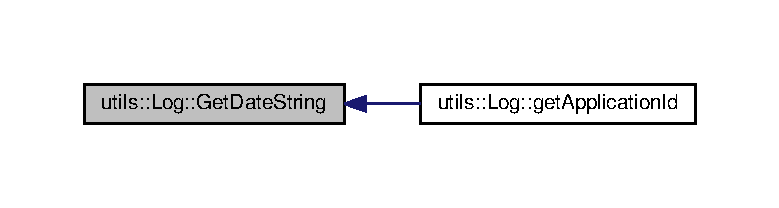
\includegraphics[width=350pt]{classutils_1_1Log_ad34711830c35c8a91b61817a0669c4f8_icgraph}
\end{center}
\end{figure}


\index{utils\+::\+Log@{utils\+::\+Log}!get\+Log\+Accs\+Client@{get\+Log\+Accs\+Client}}
\index{get\+Log\+Accs\+Client@{get\+Log\+Accs\+Client}!utils\+::\+Log@{utils\+::\+Log}}
\subsubsection[{\texorpdfstring{get\+Log\+Accs\+Client(bool createnew=false)}{getLogAccsClient(bool createnew=false)}}]{\setlength{\rightskip}{0pt plus 5cm}static void utils\+::\+Log\+::get\+Log\+Accs\+Client (
\begin{DoxyParamCaption}
\item[{bool}]{createnew = {\ttfamily false}}
\end{DoxyParamCaption}
)\hspace{0.3cm}{\ttfamily [static]}, {\ttfamily [protected]}}\hypertarget{classutils_1_1Log_afbdd825cb55cc5e13c08f347590debe9}{}\label{classutils_1_1Log_afbdd825cb55cc5e13c08f347590debe9}


Here is the caller graph for this function\+:
\nopagebreak
\begin{figure}[H]
\begin{center}
\leavevmode
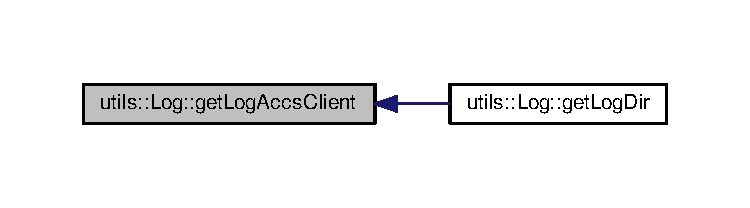
\includegraphics[width=350pt]{classutils_1_1Log_afbdd825cb55cc5e13c08f347590debe9_icgraph}
\end{center}
\end{figure}


\index{utils\+::\+Log@{utils\+::\+Log}!get\+Log\+Destination@{get\+Log\+Destination}}
\index{get\+Log\+Destination@{get\+Log\+Destination}!utils\+::\+Log@{utils\+::\+Log}}
\subsubsection[{\texorpdfstring{get\+Log\+Destination()}{getLogDestination()}}]{\setlength{\rightskip}{0pt plus 5cm}static {\bf Log\+Dest} utils\+::\+Log\+::get\+Log\+Destination (
\begin{DoxyParamCaption}
{}
\end{DoxyParamCaption}
)\hspace{0.3cm}{\ttfamily [static]}}\hypertarget{classutils_1_1Log_ad5953c44e5c56d1bd06597320f1ff684}{}\label{classutils_1_1Log_ad5953c44e5c56d1bd06597320f1ff684}


Here is the caller graph for this function\+:
\nopagebreak
\begin{figure}[H]
\begin{center}
\leavevmode
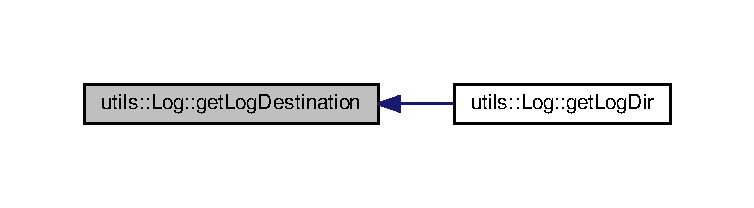
\includegraphics[width=350pt]{classutils_1_1Log_ad5953c44e5c56d1bd06597320f1ff684_icgraph}
\end{center}
\end{figure}


\index{utils\+::\+Log@{utils\+::\+Log}!get\+Log\+Destination\+String@{get\+Log\+Destination\+String}}
\index{get\+Log\+Destination\+String@{get\+Log\+Destination\+String}!utils\+::\+Log@{utils\+::\+Log}}
\subsubsection[{\texorpdfstring{get\+Log\+Destination\+String(\+Log\+Dest n\+Log\+Dest)}{getLogDestinationString(LogDest nLogDest)}}]{\setlength{\rightskip}{0pt plus 5cm}static const std\+::string utils\+::\+Log\+::get\+Log\+Destination\+String (
\begin{DoxyParamCaption}
\item[{{\bf Log\+Dest}}]{n\+Log\+Dest}
\end{DoxyParamCaption}
)\hspace{0.3cm}{\ttfamily [static]}}\hypertarget{classutils_1_1Log_a1b9c322df1f6e867cde069e02649df03}{}\label{classutils_1_1Log_a1b9c322df1f6e867cde069e02649df03}


Here is the caller graph for this function\+:
\nopagebreak
\begin{figure}[H]
\begin{center}
\leavevmode
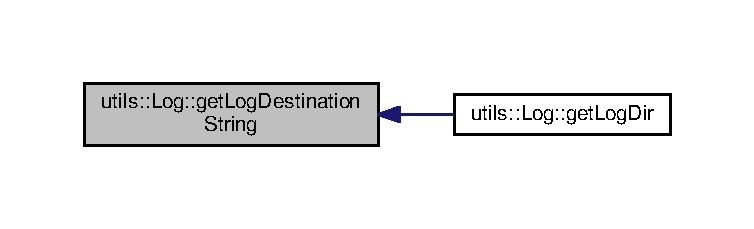
\includegraphics[width=350pt]{classutils_1_1Log_a1b9c322df1f6e867cde069e02649df03_icgraph}
\end{center}
\end{figure}


\index{utils\+::\+Log@{utils\+::\+Log}!get\+Log\+Dir@{get\+Log\+Dir}}
\index{get\+Log\+Dir@{get\+Log\+Dir}!utils\+::\+Log@{utils\+::\+Log}}
\subsubsection[{\texorpdfstring{get\+Log\+Dir()}{getLogDir()}}]{\setlength{\rightskip}{0pt plus 5cm}static const std\+::string utils\+::\+Log\+::get\+Log\+Dir (
\begin{DoxyParamCaption}
{}
\end{DoxyParamCaption}
)\hspace{0.3cm}{\ttfamily [inline]}, {\ttfamily [static]}}\hypertarget{classutils_1_1Log_a48fa60190dc3fea1f83fe40ff2457d93}{}\label{classutils_1_1Log_a48fa60190dc3fea1f83fe40ff2457d93}


Definition at line 276 of file Log.\+h.

\index{utils\+::\+Log@{utils\+::\+Log}!get\+Log\+Level\+String@{get\+Log\+Level\+String}}
\index{get\+Log\+Level\+String@{get\+Log\+Level\+String}!utils\+::\+Log@{utils\+::\+Log}}
\subsubsection[{\texorpdfstring{get\+Log\+Level\+String(\+Log\+Levels n\+Log\+Level)}{getLogLevelString(LogLevels nLogLevel)}}]{\setlength{\rightskip}{0pt plus 5cm}const string utils\+::\+Log\+::get\+Log\+Level\+String (
\begin{DoxyParamCaption}
\item[{{\bf Log\+Levels}}]{n\+Log\+Level}
\end{DoxyParamCaption}
)\hspace{0.3cm}{\ttfamily [static]}}\hypertarget{classutils_1_1Log_a779af049e980e1e02bc2e8b51d4557b1}{}\label{classutils_1_1Log_a779af049e980e1e02bc2e8b51d4557b1}


String constant holding the filename to be used if the requested file cannot be opened. 

Converts the log level enum into a string to be put in the log message 
\begin{DoxyParams}{Parameters}
{\em n\+Log\+Level} & the level assigned to this message \\
\hline
\end{DoxyParams}
\begin{DoxyReturn}{Returns}
true if this level is active, false if it is to be ignored 
\end{DoxyReturn}


Definition at line 98 of file Log.\+cpp.

\index{utils\+::\+Log@{utils\+::\+Log}!get\+String\+To\+Log\+Destination@{get\+String\+To\+Log\+Destination}}
\index{get\+String\+To\+Log\+Destination@{get\+String\+To\+Log\+Destination}!utils\+::\+Log@{utils\+::\+Log}}
\subsubsection[{\texorpdfstring{get\+String\+To\+Log\+Destination(const std\+::string \&log\+Destination)}{getStringToLogDestination(const std::string &logDestination)}}]{\setlength{\rightskip}{0pt plus 5cm}static const {\bf Log\+Dest} utils\+::\+Log\+::get\+String\+To\+Log\+Destination (
\begin{DoxyParamCaption}
\item[{const std\+::string \&}]{log\+Destination}
\end{DoxyParamCaption}
)\hspace{0.3cm}{\ttfamily [static]}}\hypertarget{classutils_1_1Log_a475ccc5ab88a7b288aaa89d67220c2b4}{}\label{classutils_1_1Log_a475ccc5ab88a7b288aaa89d67220c2b4}


Here is the caller graph for this function\+:
\nopagebreak
\begin{figure}[H]
\begin{center}
\leavevmode
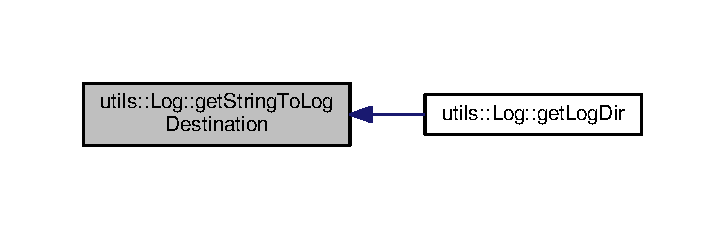
\includegraphics[width=348pt]{classutils_1_1Log_a475ccc5ab88a7b288aaa89d67220c2b4_icgraph}
\end{center}
\end{figure}


\index{utils\+::\+Log@{utils\+::\+Log}!get\+String\+To\+Log\+Level@{get\+String\+To\+Log\+Level}}
\index{get\+String\+To\+Log\+Level@{get\+String\+To\+Log\+Level}!utils\+::\+Log@{utils\+::\+Log}}
\subsubsection[{\texorpdfstring{get\+String\+To\+Log\+Level(const std\+::string \&log\+Level)}{getStringToLogLevel(const std::string &logLevel)}}]{\setlength{\rightskip}{0pt plus 5cm}const {\bf Log\+::\+Log\+Levels} utils\+::\+Log\+::get\+String\+To\+Log\+Level (
\begin{DoxyParamCaption}
\item[{const std\+::string \&}]{log\+Level}
\end{DoxyParamCaption}
)\hspace{0.3cm}{\ttfamily [static]}}\hypertarget{classutils_1_1Log_aa6c0a789ec50e1c59c4598e0a5436c2d}{}\label{classutils_1_1Log_aa6c0a789ec50e1c59c4598e0a5436c2d}


Definition at line 114 of file Log.\+cpp.

\index{utils\+::\+Log@{utils\+::\+Log}!Get\+Tick\+Count@{Get\+Tick\+Count}}
\index{Get\+Tick\+Count@{Get\+Tick\+Count}!utils\+::\+Log@{utils\+::\+Log}}
\subsubsection[{\texorpdfstring{Get\+Tick\+Count()}{GetTickCount()}}]{\setlength{\rightskip}{0pt plus 5cm}static unsigned long utils\+::\+Log\+::\+Get\+Tick\+Count (
\begin{DoxyParamCaption}
{}
\end{DoxyParamCaption}
)\hspace{0.3cm}{\ttfamily [static]}}\hypertarget{classutils_1_1Log_ae8791e18abf55ade26b8bcbae0921eaf}{}\label{classutils_1_1Log_ae8791e18abf55ade26b8bcbae0921eaf}
Get Tick Count \begin{DoxyReturn}{Returns}
unsigned long tick count in milliseconds 
\end{DoxyReturn}


Here is the caller graph for this function\+:
\nopagebreak
\begin{figure}[H]
\begin{center}
\leavevmode
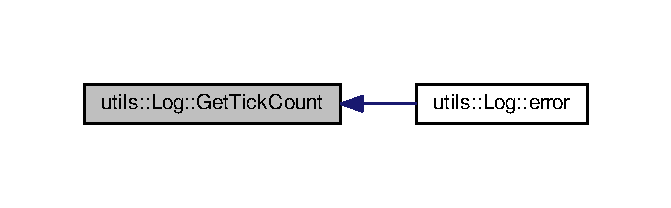
\includegraphics[width=322pt]{classutils_1_1Log_ae8791e18abf55ade26b8bcbae0921eaf_icgraph}
\end{center}
\end{figure}


\index{utils\+::\+Log@{utils\+::\+Log}!info@{info}}
\index{info@{info}!utils\+::\+Log@{utils\+::\+Log}}
\subsubsection[{\texorpdfstring{info(const char $\ast$sz\+File\+Name, const int n\+Line\+Number, const char $\ast$sz\+Msg, const char $\ast$sz\+Application\+Id=\+N\+U\+L\+L, const char $\ast$sz\+Method\+Name=\+N\+U\+L\+L, const char $\ast$sz\+Src\+Filename=\+N\+U\+L\+L, Log\+::\+Log\+Dest nlog\+Dest=\+Log\+::\+F\+I\+L\+E, bool use\+Param\+Destination=false)}{info(const char *szFileName, const int nLineNumber, const char *szMsg, const char *szApplicationId=NULL, const char *szMethodName=NULL, const char *szSrcFilename=NULL, Log::LogDest nlogDest=Log::FILE, bool useParamDestination=false)}}]{\setlength{\rightskip}{0pt plus 5cm}static void utils\+::\+Log\+::info (
\begin{DoxyParamCaption}
\item[{const char $\ast$}]{sz\+File\+Name, }
\item[{const int}]{n\+Line\+Number, }
\item[{const char $\ast$}]{sz\+Msg, }
\item[{const char $\ast$}]{sz\+Application\+Id = {\ttfamily NULL}, }
\item[{const char $\ast$}]{sz\+Method\+Name = {\ttfamily NULL}, }
\item[{const char $\ast$}]{sz\+Src\+Filename = {\ttfamily NULL}, }
\item[{{\bf Log\+::\+Log\+Dest}}]{nlog\+Dest = {\ttfamily {\bf Log\+::\+F\+I\+LE}}, }
\item[{bool}]{use\+Param\+Destination = {\ttfamily false}}
\end{DoxyParamCaption}
)\hspace{0.3cm}{\ttfamily [inline]}, {\ttfamily [static]}}\hypertarget{classutils_1_1Log_acee86547a863c04b349ab46a3b7ba9f2}{}\label{classutils_1_1Log_acee86547a863c04b349ab46a3b7ba9f2}
Send an informational message to the logging output 
\begin{DoxyParams}{Parameters}
{\em sz\+File\+Name} & file name of the file from which the log call was made \\
\hline
{\em n\+Line\+Number} & line number within the source file \\
\hline
{\em sz\+Msg} & message string to be logged \\
\hline
{\em sz\+Application\+Id} & application id from which the log call was made (used to construct log file name). Defaults to value set on init \\
\hline
{\em sz\+Application\+Id} & application id from which the log call was made (used to construct log file name). Defaults to value set on init \\
\hline
{\em sz\+Method\+Name} & the method name from where this function has been called \\
\hline
{\em sz\+Src\+Filename} & name of file which is getting procceses at the time of this function call \\
\hline
{\em nlog\+Dest} & which destination(file/database) the log message need to be logged \\
\hline
{\em use\+Param\+Destination} & boolean variable which says wether the log destination is passed in parameter or the dynamic config variable \\
\hline
\end{DoxyParams}
\begin{DoxyReturn}{Returns}
none 
\end{DoxyReturn}
\begin{DoxySeeAlso}{See also}
\hyperlink{classutils_1_1Log_ae5616599185aa1a607c838caa150f760}{Log\+::log} 
\end{DoxySeeAlso}


Definition at line 136 of file Log.\+h.

\index{utils\+::\+Log@{utils\+::\+Log}!init@{init}}
\index{init@{init}!utils\+::\+Log@{utils\+::\+Log}}
\subsubsection[{\texorpdfstring{init(const char $\ast$value)}{init(const char *value)}}]{\setlength{\rightskip}{0pt plus 5cm}void utils\+::\+Log\+::init (
\begin{DoxyParamCaption}
\item[{const char $\ast$}]{value}
\end{DoxyParamCaption}
)\hspace{0.3cm}{\ttfamily [static]}}\hypertarget{classutils_1_1Log_a78fee29378f2064f9ee8299cb59d26ce}{}\label{classutils_1_1Log_a78fee29378f2064f9ee8299cb59d26ce}


Deprecated methods (Remove as soon as possible) /////. 

Initialise logging with the application id to be used to construct the log file 
\begin{DoxyParams}{Parameters}
{\em value} & application id from which the log call was made \\
\hline
\end{DoxyParams}
\begin{DoxyReturn}{Returns}
none 
\end{DoxyReturn}


Definition at line 298 of file Log.\+cpp.



Here is the caller graph for this function\+:
\nopagebreak
\begin{figure}[H]
\begin{center}
\leavevmode
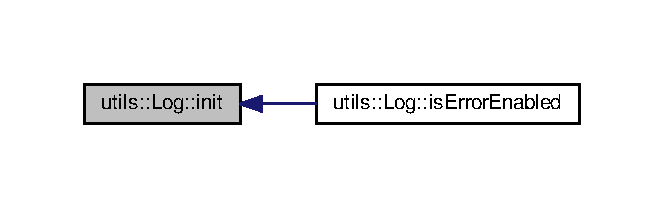
\includegraphics[width=318pt]{classutils_1_1Log_a78fee29378f2064f9ee8299cb59d26ce_icgraph}
\end{center}
\end{figure}


\index{utils\+::\+Log@{utils\+::\+Log}!init@{init}}
\index{init@{init}!utils\+::\+Log@{utils\+::\+Log}}
\subsubsection[{\texorpdfstring{init(const char $\ast$logapp, const char $\ast$logdir, const Log\+Levels prio\+Lvl, const bool flag)}{init(const char *logapp, const char *logdir, const LogLevels prioLvl, const bool flag)}}]{\setlength{\rightskip}{0pt plus 5cm}void utils\+::\+Log\+::init (
\begin{DoxyParamCaption}
\item[{const char $\ast$}]{logapp, }
\item[{const char $\ast$}]{logdir, }
\item[{const {\bf Log\+Levels}}]{prio\+Lvl, }
\item[{const bool}]{flag}
\end{DoxyParamCaption}
)\hspace{0.3cm}{\ttfamily [static]}}\hypertarget{classutils_1_1Log_a0a94150091c4d2768da2eac92006bdc7}{}\label{classutils_1_1Log_a0a94150091c4d2768da2eac92006bdc7}


Definition at line 60 of file Log.\+cpp.

\index{utils\+::\+Log@{utils\+::\+Log}!init\+Done@{init\+Done}}
\index{init\+Done@{init\+Done}!utils\+::\+Log@{utils\+::\+Log}}
\subsubsection[{\texorpdfstring{init\+Done()}{initDone()}}]{\setlength{\rightskip}{0pt plus 5cm}static bool utils\+::\+Log\+::init\+Done (
\begin{DoxyParamCaption}
{}
\end{DoxyParamCaption}
)\hspace{0.3cm}{\ttfamily [inline]}, {\ttfamily [static]}}\hypertarget{classutils_1_1Log_a17b6d2bfbc21f2aa5af7815a1c2ca166}{}\label{classutils_1_1Log_a17b6d2bfbc21f2aa5af7815a1c2ca166}
Checks to see if init called \begin{DoxyReturn}{Returns}
true if initialise has been called, false if not 
\end{DoxyReturn}


Definition at line 257 of file Log.\+h.

\index{utils\+::\+Log@{utils\+::\+Log}!is\+Error\+Enabled@{is\+Error\+Enabled}}
\index{is\+Error\+Enabled@{is\+Error\+Enabled}!utils\+::\+Log@{utils\+::\+Log}}
\subsubsection[{\texorpdfstring{is\+Error\+Enabled()}{isErrorEnabled()}}]{\setlength{\rightskip}{0pt plus 5cm}static bool utils\+::\+Log\+::is\+Error\+Enabled (
\begin{DoxyParamCaption}
{}
\end{DoxyParamCaption}
)\hspace{0.3cm}{\ttfamily [inline]}, {\ttfamily [static]}}\hypertarget{classutils_1_1Log_ac8b80b98cd9f5de11e53980a873862a4}{}\label{classutils_1_1Log_ac8b80b98cd9f5de11e53980a873862a4}


Definition at line 88 of file Log.\+h.

\index{utils\+::\+Log@{utils\+::\+Log}!is\+Info\+Enabled@{is\+Info\+Enabled}}
\index{is\+Info\+Enabled@{is\+Info\+Enabled}!utils\+::\+Log@{utils\+::\+Log}}
\subsubsection[{\texorpdfstring{is\+Info\+Enabled()}{isInfoEnabled()}}]{\setlength{\rightskip}{0pt plus 5cm}static bool utils\+::\+Log\+::is\+Info\+Enabled (
\begin{DoxyParamCaption}
{}
\end{DoxyParamCaption}
)\hspace{0.3cm}{\ttfamily [inline]}, {\ttfamily [static]}}\hypertarget{classutils_1_1Log_af831fb2def9d0984c712ca6c73cf2cd8}{}\label{classutils_1_1Log_af831fb2def9d0984c712ca6c73cf2cd8}


Definition at line 86 of file Log.\+h.

\index{utils\+::\+Log@{utils\+::\+Log}!is\+Trace\+Enabled@{is\+Trace\+Enabled}}
\index{is\+Trace\+Enabled@{is\+Trace\+Enabled}!utils\+::\+Log@{utils\+::\+Log}}
\subsubsection[{\texorpdfstring{is\+Trace\+Enabled()}{isTraceEnabled()}}]{\setlength{\rightskip}{0pt plus 5cm}static bool utils\+::\+Log\+::is\+Trace\+Enabled (
\begin{DoxyParamCaption}
{}
\end{DoxyParamCaption}
)\hspace{0.3cm}{\ttfamily [inline]}, {\ttfamily [static]}}\hypertarget{classutils_1_1Log_ad5b43b0f5ea6a8b447407a33cda5a4bf}{}\label{classutils_1_1Log_ad5b43b0f5ea6a8b447407a33cda5a4bf}


Definition at line 85 of file Log.\+h.

\index{utils\+::\+Log@{utils\+::\+Log}!is\+Warn\+Enabled@{is\+Warn\+Enabled}}
\index{is\+Warn\+Enabled@{is\+Warn\+Enabled}!utils\+::\+Log@{utils\+::\+Log}}
\subsubsection[{\texorpdfstring{is\+Warn\+Enabled()}{isWarnEnabled()}}]{\setlength{\rightskip}{0pt plus 5cm}static bool utils\+::\+Log\+::is\+Warn\+Enabled (
\begin{DoxyParamCaption}
{}
\end{DoxyParamCaption}
)\hspace{0.3cm}{\ttfamily [inline]}, {\ttfamily [static]}}\hypertarget{classutils_1_1Log_a99a23d525a51c3290f793dedadc65470}{}\label{classutils_1_1Log_a99a23d525a51c3290f793dedadc65470}


Definition at line 87 of file Log.\+h.

\index{utils\+::\+Log@{utils\+::\+Log}!log@{log}}
\index{log@{log}!utils\+::\+Log@{utils\+::\+Log}}
\subsubsection[{\texorpdfstring{log(\+Log\+Levels n\+Log\+Level, const char $\ast$sz\+File\+Name, const int n\+Line\+Number, const char $\ast$sz\+Msg, const char $\ast$sz\+Application\+Id=\+N\+U\+L\+L, const char $\ast$sz\+Method\+Name=\+N\+U\+L\+L, const char $\ast$sz\+Src\+Filename=\+N\+U\+L\+L, Log\+::\+Log\+Dest nlog\+Dest=\+Log\+::\+F\+I\+L\+E, bool use\+Param\+Destination=false)}{log(LogLevels nLogLevel, const char *szFileName, const int nLineNumber, const char *szMsg, const char *szApplicationId=NULL, const char *szMethodName=NULL, const char *szSrcFilename=NULL, Log::LogDest nlogDest=Log::FILE, bool useParamDestination=false)}}]{\setlength{\rightskip}{0pt plus 5cm}void utils\+::\+Log\+::log (
\begin{DoxyParamCaption}
\item[{{\bf Log\+Levels}}]{n\+Log\+Level, }
\item[{const char $\ast$}]{sz\+File\+Name, }
\item[{const int}]{n\+Line\+Number, }
\item[{const char $\ast$}]{sz\+Msg, }
\item[{const char $\ast$}]{sz\+Application\+Id = {\ttfamily NULL}, }
\item[{const char $\ast$}]{sz\+Method\+Name = {\ttfamily NULL}, }
\item[{const char $\ast$}]{sz\+Src\+Filename = {\ttfamily NULL}, }
\item[{{\bf Log\+::\+Log\+Dest}}]{nlog\+Dest = {\ttfamily {\bf Log\+::\+F\+I\+LE}}, }
\item[{bool}]{use\+Param\+Destination = {\ttfamily false}}
\end{DoxyParamCaption}
)\hspace{0.3cm}{\ttfamily [static]}}\hypertarget{classutils_1_1Log_ae5616599185aa1a607c838caa150f760}{}\label{classutils_1_1Log_ae5616599185aa1a607c838caa150f760}
\hyperlink{classutils_1_1Log}{Log} a message to the defined output, if the levels are set such that this is required 
\begin{DoxyParams}{Parameters}
{\em n\+Log\+Level} & the filtering level assigned to this message \\
\hline
{\em sz\+File\+Name} & file name of the file from which the log call was made \\
\hline
{\em n\+Line\+Number} & line number within the source file \\
\hline
{\em sz\+Msg} & message string to be logged \\
\hline
{\em sz\+Application\+Id} & application id from which the log call was made (used to construct log file name). Defaults to value set on init \\
\hline
{\em sz\+Application\+Id} & application id from which the log call was made (used to construct log file name). Defaults to value set on init \\
\hline
{\em sz\+Method\+Name} & the method name from where this function has been called \\
\hline
{\em sz\+Src\+Filename} & name of file which is getting procceses at the time of this function call \\
\hline
{\em nlog\+Dest} & which destination(file/database) the log message need to be logged \\
\hline
{\em use\+Param\+Destination} & boolean variable which says wether the log destination is passed in parameter or the dynamic config variable \\
\hline
\end{DoxyParams}
\begin{DoxyReturn}{Returns}
none 
\end{DoxyReturn}
\begin{DoxySeeAlso}{See also}
Log\+::log\+Message\+To\+File 

Log\+::log\+Message\+To\+Db 
\end{DoxySeeAlso}


Definition at line 128 of file Log.\+cpp.



Here is the caller graph for this function\+:
\nopagebreak
\begin{figure}[H]
\begin{center}
\leavevmode
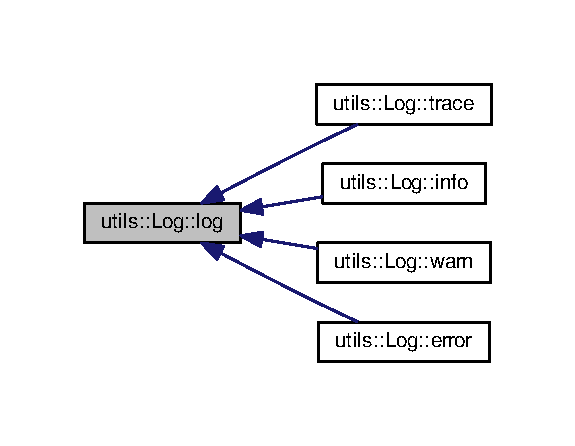
\includegraphics[width=276pt]{classutils_1_1Log_ae5616599185aa1a607c838caa150f760_icgraph}
\end{center}
\end{figure}


\index{utils\+::\+Log@{utils\+::\+Log}!log\+Elapsed\+Time@{log\+Elapsed\+Time}}
\index{log\+Elapsed\+Time@{log\+Elapsed\+Time}!utils\+::\+Log@{utils\+::\+Log}}
\subsubsection[{\texorpdfstring{log\+Elapsed\+Time(const char $\ast$sz\+Module\+Name, const int n\+Line\+Number, const char $\ast$sz\+Msg\+File\+Name, const char $\ast$sz\+Desc, const char $\ast$sz\+Call\+Id, const char $\ast$logname\+Override, Log\+::\+Log\+Dest nlog\+Dest, unsigned long \&ul\+Start\+Call, unsigned long \&ul\+Initial, int n\+Tm\+Mask, double db\+Avg\+Tm=0.\+0, bool elapsed\+Time\+Db\+Logging=false, bool use\+Param\+Destination=false)}{logElapsedTime(const char *szModuleName, const int nLineNumber, const char *szMsgFileName, const char *szDesc, const char *szCallId, const char *lognameOverride, Log::LogDest nlogDest, unsigned long &ulStartCall, unsigned long &ulInitial, int nTmMask, double dbAvgTm=0.0, bool elapsedTimeDbLogging=false, bool useParamDestination=false)}}]{\setlength{\rightskip}{0pt plus 5cm}static void utils\+::\+Log\+::log\+Elapsed\+Time (
\begin{DoxyParamCaption}
\item[{const char $\ast$}]{sz\+Module\+Name, }
\item[{const int}]{n\+Line\+Number, }
\item[{const char $\ast$}]{sz\+Msg\+File\+Name, }
\item[{const char $\ast$}]{sz\+Desc, }
\item[{const char $\ast$}]{sz\+Call\+Id, }
\item[{const char $\ast$}]{logname\+Override, }
\item[{{\bf Log\+::\+Log\+Dest}}]{nlog\+Dest, }
\item[{unsigned long \&}]{ul\+Start\+Call, }
\item[{unsigned long \&}]{ul\+Initial, }
\item[{int}]{n\+Tm\+Mask, }
\item[{double}]{db\+Avg\+Tm = {\ttfamily 0.0}, }
\item[{bool}]{elapsed\+Time\+Db\+Logging = {\ttfamily false}, }
\item[{bool}]{use\+Param\+Destination = {\ttfamily false}}
\end{DoxyParamCaption}
)\hspace{0.3cm}{\ttfamily [static]}}\hypertarget{classutils_1_1Log_a3288f62f0edee03354f3c258aabccae3}{}\label{classutils_1_1Log_a3288f62f0edee03354f3c258aabccae3}
Write the elapsed time log message to a file using the description 
\begin{DoxyParams}{Parameters}
{\em sz\+Module\+Name} & file name of the code module from which the log call was made \\
\hline
{\em n\+Line\+Number} & line number within the source file \\
\hline
{\em sz\+Msg\+File\+Name} & file name of message being processed \\
\hline
{\em sz\+Desc} & message description \\
\hline
{\em sz\+Call\+Id} & name of method for which the elapsed time applies \\
\hline
{\em sz\+Logname\+Override} & Overrides the default logname with the specified logname \\
\hline
{\em ul\+Start\+Call} & starting time for call \\
\hline
{\em ul\+Initial} & initial starting time for current processing stage \\
\hline
{\em n\+Tm\+Mask} & Mask which determines whether to output elapsed time or not \\
\hline
{\em db\+Avg\+Tm} & Time to use for out of range calculations \\
\hline
\end{DoxyParams}
\begin{DoxyReturn}{Returns}
none 
\end{DoxyReturn}


Here is the caller graph for this function\+:
\nopagebreak
\begin{figure}[H]
\begin{center}
\leavevmode
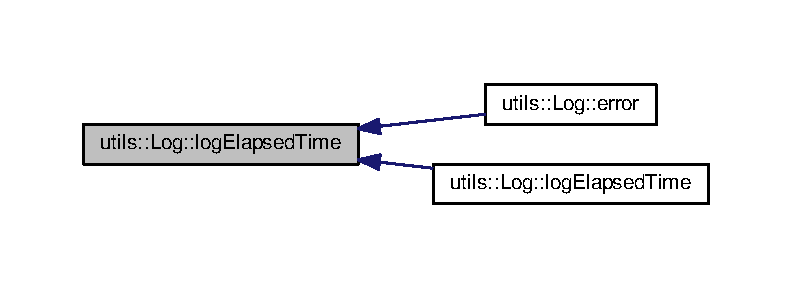
\includegraphics[width=350pt]{classutils_1_1Log_a3288f62f0edee03354f3c258aabccae3_icgraph}
\end{center}
\end{figure}


\index{utils\+::\+Log@{utils\+::\+Log}!log\+Elapsed\+Time@{log\+Elapsed\+Time}}
\index{log\+Elapsed\+Time@{log\+Elapsed\+Time}!utils\+::\+Log@{utils\+::\+Log}}
\subsubsection[{\texorpdfstring{log\+Elapsed\+Time(const char $\ast$sz\+Module\+Name, const int n\+Line\+Number, const char $\ast$sz\+Msg\+File\+Name, const char $\ast$sz\+Desc, const char $\ast$sz\+Call\+Id, unsigned long \&ul\+Start\+Call, unsigned long \&ul\+Initial, int n\+Tm\+Mask, double db\+Avg\+Tm=0.\+0)}{logElapsedTime(const char *szModuleName, const int nLineNumber, const char *szMsgFileName, const char *szDesc, const char *szCallId, unsigned long &ulStartCall, unsigned long &ulInitial, int nTmMask, double dbAvgTm=0.0)}}]{\setlength{\rightskip}{0pt plus 5cm}static void utils\+::\+Log\+::log\+Elapsed\+Time (
\begin{DoxyParamCaption}
\item[{const char $\ast$}]{sz\+Module\+Name, }
\item[{const int}]{n\+Line\+Number, }
\item[{const char $\ast$}]{sz\+Msg\+File\+Name, }
\item[{const char $\ast$}]{sz\+Desc, }
\item[{const char $\ast$}]{sz\+Call\+Id, }
\item[{unsigned long \&}]{ul\+Start\+Call, }
\item[{unsigned long \&}]{ul\+Initial, }
\item[{int}]{n\+Tm\+Mask, }
\item[{double}]{db\+Avg\+Tm = {\ttfamily 0.0}}
\end{DoxyParamCaption}
)\hspace{0.3cm}{\ttfamily [inline]}, {\ttfamily [static]}}\hypertarget{classutils_1_1Log_a42cc9a0f0ecd76abd678ebd7ac59d8d7}{}\label{classutils_1_1Log_a42cc9a0f0ecd76abd678ebd7ac59d8d7}
Calls log\+Elapsed\+Time(...) with the following defaults 
\begin{DoxyParams}{Parameters}
{\em sz\+Logname\+Override} & parameter defaulted to N\+U\+LL \\
\hline
{\em nlog\+Dest} & parameter defaulted to N\+O\+NE \\
\hline
\end{DoxyParams}


Definition at line 233 of file Log.\+h.

\index{utils\+::\+Log@{utils\+::\+Log}!log\+Elapsed\+Time@{log\+Elapsed\+Time}}
\index{log\+Elapsed\+Time@{log\+Elapsed\+Time}!utils\+::\+Log@{utils\+::\+Log}}
\subsubsection[{\texorpdfstring{log\+Elapsed\+Time(const char $\ast$sz\+Module\+Name, const int n\+Line\+Number, const char $\ast$sz\+Msg\+File\+Name, const char $\ast$sz\+Desc, const char $\ast$sz\+Call\+Id, Log\+::\+Log\+Dest nlog\+Dest, unsigned long \&ul\+Start\+Call, unsigned long \&ul\+Initial, int n\+Tm\+Mask, double db\+Avg\+Tm=0.\+0)}{logElapsedTime(const char *szModuleName, const int nLineNumber, const char *szMsgFileName, const char *szDesc, const char *szCallId, Log::LogDest nlogDest, unsigned long &ulStartCall, unsigned long &ulInitial, int nTmMask, double dbAvgTm=0.0)}}]{\setlength{\rightskip}{0pt plus 5cm}static void utils\+::\+Log\+::log\+Elapsed\+Time (
\begin{DoxyParamCaption}
\item[{const char $\ast$}]{sz\+Module\+Name, }
\item[{const int}]{n\+Line\+Number, }
\item[{const char $\ast$}]{sz\+Msg\+File\+Name, }
\item[{const char $\ast$}]{sz\+Desc, }
\item[{const char $\ast$}]{sz\+Call\+Id, }
\item[{{\bf Log\+::\+Log\+Dest}}]{nlog\+Dest, }
\item[{unsigned long \&}]{ul\+Start\+Call, }
\item[{unsigned long \&}]{ul\+Initial, }
\item[{int}]{n\+Tm\+Mask, }
\item[{double}]{db\+Avg\+Tm = {\ttfamily 0.0}}
\end{DoxyParamCaption}
)\hspace{0.3cm}{\ttfamily [inline]}, {\ttfamily [static]}}\hypertarget{classutils_1_1Log_ab7985810504b1e575a408a3fc14118d0}{}\label{classutils_1_1Log_ab7985810504b1e575a408a3fc14118d0}
Calls log\+Elapsed\+Time(...) with the following defaults 
\begin{DoxyParams}{Parameters}
{\em sz\+Logname\+Override} & parameter defaulted to N\+U\+LL \\
\hline
\end{DoxyParams}


Definition at line 245 of file Log.\+h.

\index{utils\+::\+Log@{utils\+::\+Log}!log\+Message\+To\+File@{log\+Message\+To\+File}}
\index{log\+Message\+To\+File@{log\+Message\+To\+File}!utils\+::\+Log@{utils\+::\+Log}}
\subsubsection[{\texorpdfstring{log\+Message\+To\+File()}{logMessageToFile()}}]{\setlength{\rightskip}{0pt plus 5cm}static void utils\+::\+Log\+::log\+Message\+To\+File (
\begin{DoxyParamCaption}
{}
\end{DoxyParamCaption}
)\hspace{0.3cm}{\ttfamily [static]}}\hypertarget{classutils_1_1Log_ac526c9aee25389e092ba27c5f5feb3e8}{}\label{classutils_1_1Log_ac526c9aee25389e092ba27c5f5feb3e8}


Here is the caller graph for this function\+:
\nopagebreak
\begin{figure}[H]
\begin{center}
\leavevmode
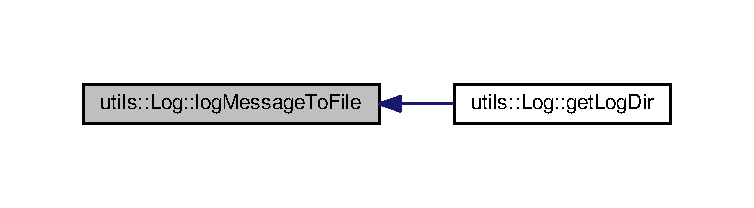
\includegraphics[width=350pt]{classutils_1_1Log_ac526c9aee25389e092ba27c5f5feb3e8_icgraph}
\end{center}
\end{figure}


\index{utils\+::\+Log@{utils\+::\+Log}!set\+Elapsed@{set\+Elapsed}}
\index{set\+Elapsed@{set\+Elapsed}!utils\+::\+Log@{utils\+::\+Log}}
\subsubsection[{\texorpdfstring{set\+Elapsed(char $\ast$value, int mask)}{setElapsed(char *value, int mask)}}]{\setlength{\rightskip}{0pt plus 5cm}static void utils\+::\+Log\+::set\+Elapsed (
\begin{DoxyParamCaption}
\item[{char $\ast$}]{value, }
\item[{int}]{mask}
\end{DoxyParamCaption}
)\hspace{0.3cm}{\ttfamily [static]}}\hypertarget{classutils_1_1Log_aecbaeed2809b1cf54b5d78fbc9870ebe}{}\label{classutils_1_1Log_aecbaeed2809b1cf54b5d78fbc9870ebe}
Initialise / reset elapsed data fields 
\begin{DoxyParams}{Parameters}
{\em value} & logname \\
\hline
{\em mask} & elapsed mask \\
\hline
\end{DoxyParams}
\begin{DoxyReturn}{Returns}
none 
\end{DoxyReturn}


Here is the caller graph for this function\+:
\nopagebreak
\begin{figure}[H]
\begin{center}
\leavevmode
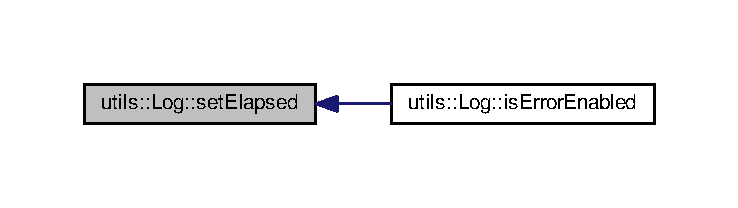
\includegraphics[width=350pt]{classutils_1_1Log_aecbaeed2809b1cf54b5d78fbc9870ebe_icgraph}
\end{center}
\end{figure}


\index{utils\+::\+Log@{utils\+::\+Log}!set\+Input\+Source\+File@{set\+Input\+Source\+File}}
\index{set\+Input\+Source\+File@{set\+Input\+Source\+File}!utils\+::\+Log@{utils\+::\+Log}}
\subsubsection[{\texorpdfstring{set\+Input\+Source\+File(std\+::string src\+File)}{setInputSourceFile(std::string srcFile)}}]{\setlength{\rightskip}{0pt plus 5cm}static void utils\+::\+Log\+::set\+Input\+Source\+File (
\begin{DoxyParamCaption}
\item[{std\+::string}]{src\+File}
\end{DoxyParamCaption}
)\hspace{0.3cm}{\ttfamily [inline]}, {\ttfamily [static]}}\hypertarget{classutils_1_1Log_a0d68bc67c1342672dc265bf16149b119}{}\label{classutils_1_1Log_a0d68bc67c1342672dc265bf16149b119}


Definition at line 349 of file Log.\+h.

\index{utils\+::\+Log@{utils\+::\+Log}!set\+Log\+Destination@{set\+Log\+Destination}}
\index{set\+Log\+Destination@{set\+Log\+Destination}!utils\+::\+Log@{utils\+::\+Log}}
\subsubsection[{\texorpdfstring{set\+Log\+Destination(\+Log\+Dest dest)}{setLogDestination(LogDest dest)}}]{\setlength{\rightskip}{0pt plus 5cm}static void utils\+::\+Log\+::set\+Log\+Destination (
\begin{DoxyParamCaption}
\item[{{\bf Log\+Dest}}]{dest}
\end{DoxyParamCaption}
)\hspace{0.3cm}{\ttfamily [static]}}\hypertarget{classutils_1_1Log_a9bc0e1c6ce4e14943da1e94a36833b59}{}\label{classutils_1_1Log_a9bc0e1c6ce4e14943da1e94a36833b59}


Here is the caller graph for this function\+:
\nopagebreak
\begin{figure}[H]
\begin{center}
\leavevmode
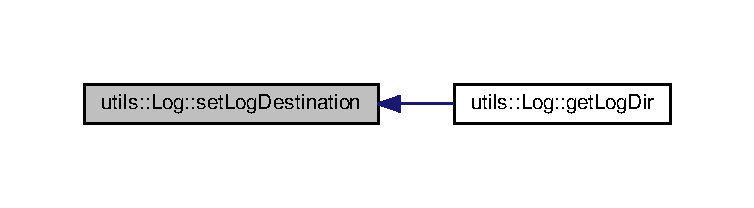
\includegraphics[width=350pt]{classutils_1_1Log_a9bc0e1c6ce4e14943da1e94a36833b59_icgraph}
\end{center}
\end{figure}


\index{utils\+::\+Log@{utils\+::\+Log}!strip\+File\+Name@{strip\+File\+Name}}
\index{strip\+File\+Name@{strip\+File\+Name}!utils\+::\+Log@{utils\+::\+Log}}
\subsubsection[{\texorpdfstring{strip\+File\+Name(const std\+::string \&sz\+Original\+File\+Name, bool strip\+Ext\+Flag=false)}{stripFileName(const std::string &szOriginalFileName, bool stripExtFlag=false)}}]{\setlength{\rightskip}{0pt plus 5cm}const string utils\+::\+Log\+::strip\+File\+Name (
\begin{DoxyParamCaption}
\item[{const std\+::string \&}]{sz\+Original\+File\+Name, }
\item[{bool}]{strip\+Ext\+Flag = {\ttfamily false}}
\end{DoxyParamCaption}
)\hspace{0.3cm}{\ttfamily [static]}}\hypertarget{classutils_1_1Log_a20b001de07bd7b008126037bed0d1393}{}\label{classutils_1_1Log_a20b001de07bd7b008126037bed0d1393}
Strip any path component off the file name 
\begin{DoxyParams}{Parameters}
{\em sz\+Original\+File\+Name} & name of the source file generating this log message \\
\hline
\end{DoxyParams}
\begin{DoxyReturn}{Returns}
Basename of the file 
\end{DoxyReturn}


Definition at line 184 of file Log.\+cpp.



Here is the caller graph for this function\+:
\nopagebreak
\begin{figure}[H]
\begin{center}
\leavevmode
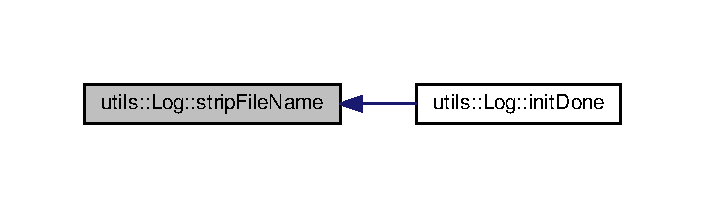
\includegraphics[width=338pt]{classutils_1_1Log_a20b001de07bd7b008126037bed0d1393_icgraph}
\end{center}
\end{figure}


\index{utils\+::\+Log@{utils\+::\+Log}!trace@{trace}}
\index{trace@{trace}!utils\+::\+Log@{utils\+::\+Log}}
\subsubsection[{\texorpdfstring{trace(const char $\ast$sz\+File\+Name, const int n\+Line\+Number, const char $\ast$sz\+Msg, const char $\ast$sz\+Application\+Id=\+N\+U\+L\+L, const char $\ast$sz\+Method\+Name=\+N\+U\+L\+L, const char $\ast$sz\+Src\+Filename=\+N\+U\+L\+L, Log\+::\+Log\+Dest nlog\+Dest=\+Log\+::\+F\+I\+L\+E, bool use\+Param\+Destination=false)}{trace(const char *szFileName, const int nLineNumber, const char *szMsg, const char *szApplicationId=NULL, const char *szMethodName=NULL, const char *szSrcFilename=NULL, Log::LogDest nlogDest=Log::FILE, bool useParamDestination=false)}}]{\setlength{\rightskip}{0pt plus 5cm}static void utils\+::\+Log\+::trace (
\begin{DoxyParamCaption}
\item[{const char $\ast$}]{sz\+File\+Name, }
\item[{const int}]{n\+Line\+Number, }
\item[{const char $\ast$}]{sz\+Msg, }
\item[{const char $\ast$}]{sz\+Application\+Id = {\ttfamily NULL}, }
\item[{const char $\ast$}]{sz\+Method\+Name = {\ttfamily NULL}, }
\item[{const char $\ast$}]{sz\+Src\+Filename = {\ttfamily NULL}, }
\item[{{\bf Log\+::\+Log\+Dest}}]{nlog\+Dest = {\ttfamily {\bf Log\+::\+F\+I\+LE}}, }
\item[{bool}]{use\+Param\+Destination = {\ttfamily false}}
\end{DoxyParamCaption}
)\hspace{0.3cm}{\ttfamily [inline]}, {\ttfamily [static]}}\hypertarget{classutils_1_1Log_a37ae89eca0ad705c5e948710406e2054}{}\label{classutils_1_1Log_a37ae89eca0ad705c5e948710406e2054}
Send a trace (debug) level message to the logging output with override for the application id 
\begin{DoxyParams}{Parameters}
{\em sz\+File\+Name} & file name of the file from which the log call was made \\
\hline
{\em n\+Line\+Number} & line number within the source file \\
\hline
{\em sz\+Msg} & message string to be logged \\
\hline
{\em sz\+Application\+Id} & application id from which the log call was made (used to construct log file name). Defaults to value set on init \\
\hline
{\em sz\+Method\+Name} & the method name from where this function has been called \\
\hline
{\em sz\+Src\+Filename} & name of file which is getting procceses at the time of this function call \\
\hline
{\em nlog\+Dest} & which destination(file/database) the log message need to be logged \\
\hline
{\em use\+Param\+Destination} & boolean variable which says wether the log destination is passed in parameter or the dynamic config variable \\
\hline
\end{DoxyParams}
\begin{DoxyReturn}{Returns}
none 
\end{DoxyReturn}
\begin{DoxySeeAlso}{See also}
\hyperlink{classutils_1_1Log_ae5616599185aa1a607c838caa150f760}{Log\+::log} 
\end{DoxySeeAlso}


Definition at line 119 of file Log.\+h.

\index{utils\+::\+Log@{utils\+::\+Log}!warn@{warn}}
\index{warn@{warn}!utils\+::\+Log@{utils\+::\+Log}}
\subsubsection[{\texorpdfstring{warn(const char $\ast$sz\+File\+Name, const int n\+Line\+Number, const char $\ast$sz\+Msg, const char $\ast$sz\+Application\+Id=\+N\+U\+L\+L, const char $\ast$sz\+Method\+Name=\+N\+U\+L\+L, const char $\ast$sz\+Src\+Filename=\+N\+U\+L\+L, Log\+::\+Log\+Dest nlog\+Dest=\+Log\+::\+F\+I\+L\+E, bool use\+Param\+Destination=false)}{warn(const char *szFileName, const int nLineNumber, const char *szMsg, const char *szApplicationId=NULL, const char *szMethodName=NULL, const char *szSrcFilename=NULL, Log::LogDest nlogDest=Log::FILE, bool useParamDestination=false)}}]{\setlength{\rightskip}{0pt plus 5cm}static void utils\+::\+Log\+::warn (
\begin{DoxyParamCaption}
\item[{const char $\ast$}]{sz\+File\+Name, }
\item[{const int}]{n\+Line\+Number, }
\item[{const char $\ast$}]{sz\+Msg, }
\item[{const char $\ast$}]{sz\+Application\+Id = {\ttfamily NULL}, }
\item[{const char $\ast$}]{sz\+Method\+Name = {\ttfamily NULL}, }
\item[{const char $\ast$}]{sz\+Src\+Filename = {\ttfamily NULL}, }
\item[{{\bf Log\+::\+Log\+Dest}}]{nlog\+Dest = {\ttfamily {\bf Log\+::\+F\+I\+LE}}, }
\item[{bool}]{use\+Param\+Destination = {\ttfamily false}}
\end{DoxyParamCaption}
)\hspace{0.3cm}{\ttfamily [inline]}, {\ttfamily [static]}}\hypertarget{classutils_1_1Log_aaff384f2d48d78b72b9c5e72ebed18db}{}\label{classutils_1_1Log_aaff384f2d48d78b72b9c5e72ebed18db}
Send a warning message to the logging output -\/ recoverable error condition 
\begin{DoxyParams}{Parameters}
{\em sz\+File\+Name} & file name of the file from which the log call was made \\
\hline
{\em n\+Line\+Number} & line number within the source file \\
\hline
{\em sz\+Msg} & message string to be logged \\
\hline
{\em sz\+Application\+Id} & application id from which the log call was made (used to construct log file name). Defaults to value set on init \\
\hline
{\em sz\+Application\+Id} & application id from which the log call was made (used to construct log file name). Defaults to value set on init \\
\hline
{\em sz\+Method\+Name} & the method name from where this function has been called \\
\hline
{\em sz\+Src\+Filename} & name of file which is getting procceses at the time of this function call \\
\hline
{\em nlog\+Dest} & which destination(file/database) the log message need to be logged \\
\hline
{\em use\+Param\+Destination} & boolean variable which says wether the log destination is passed in parameter or the dynamic config variable \\
\hline
\end{DoxyParams}
\begin{DoxyReturn}{Returns}
none 
\end{DoxyReturn}
\begin{DoxySeeAlso}{See also}
\hyperlink{classutils_1_1Log_ae5616599185aa1a607c838caa150f760}{Log\+::log} 
\end{DoxySeeAlso}


Definition at line 153 of file Log.\+h.



\subsection{Member Data Documentation}
\index{utils\+::\+Log@{utils\+::\+Log}!D\+E\+F\+A\+U\+L\+T\+\_\+\+L\+O\+G\+\_\+\+F\+I\+L\+E\+N\+A\+ME@{D\+E\+F\+A\+U\+L\+T\+\_\+\+L\+O\+G\+\_\+\+F\+I\+L\+E\+N\+A\+ME}}
\index{D\+E\+F\+A\+U\+L\+T\+\_\+\+L\+O\+G\+\_\+\+F\+I\+L\+E\+N\+A\+ME@{D\+E\+F\+A\+U\+L\+T\+\_\+\+L\+O\+G\+\_\+\+F\+I\+L\+E\+N\+A\+ME}!utils\+::\+Log@{utils\+::\+Log}}
\subsubsection[{\texorpdfstring{D\+E\+F\+A\+U\+L\+T\+\_\+\+L\+O\+G\+\_\+\+F\+I\+L\+E\+N\+A\+ME}{DEFAULT_LOG_FILENAME}}]{\setlength{\rightskip}{0pt plus 5cm}const std\+::string utils\+::\+Log\+::\+D\+E\+F\+A\+U\+L\+T\+\_\+\+L\+O\+G\+\_\+\+F\+I\+L\+E\+N\+A\+ME = \char`\"{}/tmp/hcu\+\_\+error.\+log\char`\"{}\hspace{0.3cm}{\ttfamily [static]}}\hypertarget{classutils_1_1Log_a887edb129af7794c19cf05ade96f892d}{}\label{classutils_1_1Log_a887edb129af7794c19cf05ade96f892d}


Definition at line 266 of file Log.\+h.



The documentation for this class was generated from the following files\+:\begin{DoxyCompactItemize}
\item 
L\+O\+G/\hyperlink{Log_8h}{Log.\+h}\item 
L\+O\+G/\hyperlink{Log_8cpp}{Log.\+cpp}\end{DoxyCompactItemize}

\hypertarget{classLoginAgent}{}\section{Login\+Agent Class Reference}
\label{classLoginAgent}\index{Login\+Agent@{Login\+Agent}}


{\ttfamily \#include $<$Login\+Agent.\+h$>$}

\subsection*{Public Member Functions}
\begin{DoxyCompactItemize}
\item 
void \hyperlink{classLoginAgent_a670d5b47ae1ed387f66781ae4b3a9f0c}{login} (string str\+Tag\+Name)
\item 
void \hyperlink{classLoginAgent_ababd52a019dcec0ea12d5a8f4fbea7ff}{logout} (string str\+Tag\+Name)
\item 
bool \hyperlink{classLoginAgent_a0688ca0f5cbf3daf3ed9af699774d5f3}{is\+D\+B\+Connection\+Alive} (string str\+Tag\+Name)
\end{DoxyCompactItemize}
\subsection*{Static Public Member Functions}
\begin{DoxyCompactItemize}
\item 
static \hyperlink{classLoginAgent}{Login\+Agent} $\ast$ \hyperlink{classLoginAgent_a77e0224354a90e78193bcd1110c7af37}{get\+Instance} ()
\end{DoxyCompactItemize}


\subsection{Detailed Description}


Definition at line 18 of file Login\+Agent.\+h.



\subsection{Member Function Documentation}
\index{Login\+Agent@{Login\+Agent}!get\+Instance@{get\+Instance}}
\index{get\+Instance@{get\+Instance}!Login\+Agent@{Login\+Agent}}
\subsubsection[{\texorpdfstring{get\+Instance()}{getInstance()}}]{\setlength{\rightskip}{0pt plus 5cm}static {\bf Login\+Agent}$\ast$ Login\+Agent\+::get\+Instance (
\begin{DoxyParamCaption}
{}
\end{DoxyParamCaption}
)\hspace{0.3cm}{\ttfamily [static]}}\hypertarget{classLoginAgent_a77e0224354a90e78193bcd1110c7af37}{}\label{classLoginAgent_a77e0224354a90e78193bcd1110c7af37}
\index{Login\+Agent@{Login\+Agent}!is\+D\+B\+Connection\+Alive@{is\+D\+B\+Connection\+Alive}}
\index{is\+D\+B\+Connection\+Alive@{is\+D\+B\+Connection\+Alive}!Login\+Agent@{Login\+Agent}}
\subsubsection[{\texorpdfstring{is\+D\+B\+Connection\+Alive(string str\+Tag\+Name)}{isDBConnectionAlive(string strTagName)}}]{\setlength{\rightskip}{0pt plus 5cm}bool Login\+Agent\+::is\+D\+B\+Connection\+Alive (
\begin{DoxyParamCaption}
\item[{string}]{str\+Tag\+Name}
\end{DoxyParamCaption}
)}\hypertarget{classLoginAgent_a0688ca0f5cbf3daf3ed9af699774d5f3}{}\label{classLoginAgent_a0688ca0f5cbf3daf3ed9af699774d5f3}
\index{Login\+Agent@{Login\+Agent}!login@{login}}
\index{login@{login}!Login\+Agent@{Login\+Agent}}
\subsubsection[{\texorpdfstring{login(string str\+Tag\+Name)}{login(string strTagName)}}]{\setlength{\rightskip}{0pt plus 5cm}void Login\+Agent\+::login (
\begin{DoxyParamCaption}
\item[{string}]{str\+Tag\+Name}
\end{DoxyParamCaption}
)}\hypertarget{classLoginAgent_a670d5b47ae1ed387f66781ae4b3a9f0c}{}\label{classLoginAgent_a670d5b47ae1ed387f66781ae4b3a9f0c}
\index{Login\+Agent@{Login\+Agent}!logout@{logout}}
\index{logout@{logout}!Login\+Agent@{Login\+Agent}}
\subsubsection[{\texorpdfstring{logout(string str\+Tag\+Name)}{logout(string strTagName)}}]{\setlength{\rightskip}{0pt plus 5cm}void Login\+Agent\+::logout (
\begin{DoxyParamCaption}
\item[{string}]{str\+Tag\+Name}
\end{DoxyParamCaption}
)}\hypertarget{classLoginAgent_ababd52a019dcec0ea12d5a8f4fbea7ff}{}\label{classLoginAgent_ababd52a019dcec0ea12d5a8f4fbea7ff}


The documentation for this class was generated from the following file\+:\begin{DoxyCompactItemize}
\item 
D\+Y\+N\+\_\+\+C\+O\+N\+F\+I\+G/include/\hyperlink{LoginAgent_8h}{Login\+Agent.\+h}\end{DoxyCompactItemize}

\hypertarget{classipc_1_1Pipe}{}\section{ipc\+:\+:Pipe Class Reference}
\label{classipc_1_1Pipe}\index{ipc\+::\+Pipe@{ipc\+::\+Pipe}}


{\ttfamily \#include $<$Pipe.\+h$>$}



Inheritance diagram for ipc\+:\+:Pipe\+:
\nopagebreak
\begin{figure}[H]
\begin{center}
\leavevmode
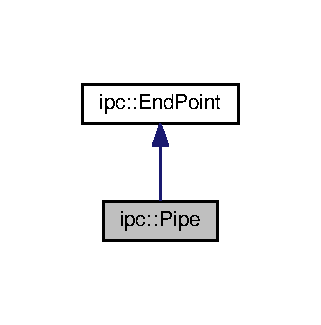
\includegraphics[width=154pt]{classipc_1_1Pipe__inherit__graph}
\end{center}
\end{figure}


Collaboration diagram for ipc\+:\+:Pipe\+:
\nopagebreak
\begin{figure}[H]
\begin{center}
\leavevmode
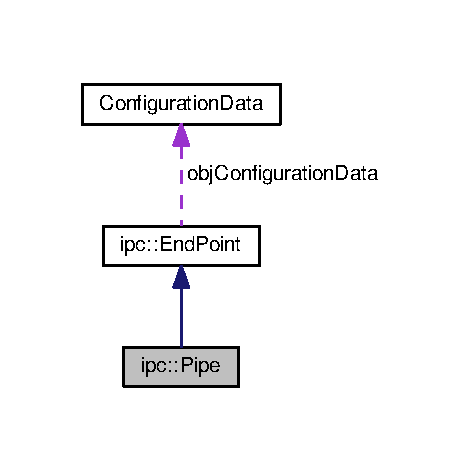
\includegraphics[width=222pt]{classipc_1_1Pipe__coll__graph}
\end{center}
\end{figure}
\subsection*{Public Member Functions}
\begin{DoxyCompactItemize}
\item 
\hyperlink{classipc_1_1Pipe_a91ddad07e89d5585b1cf27fa7860e201}{Pipe} ()
\item 
virtual \hyperlink{classipc_1_1Pipe_af4519cc3f1f13857a724db7b2220eefa}{$\sim$\+Pipe} ()
\item 
void \hyperlink{classipc_1_1Pipe_adbae487d0da061626a372cf4b8dd9b39}{initialize} (string str\+Name=\char`\"{}\char`\"{})
\item 
Emp\+Full\+Message $\ast$ \hyperlink{classipc_1_1Pipe_ac48948dba8e24c66d85c54594a813065}{read\+Data} ()
\item 
void \hyperlink{classipc_1_1Pipe_aa9d1114a883aef079d9f0d8d11fdd377}{write\+Data} (Emp\+Full\+Message $\ast$message)
\item 
void \hyperlink{classipc_1_1Pipe_a3f1de71c9add87611319d2838404dce3}{destroy} ()
\item 
bool \hyperlink{classipc_1_1Pipe_ab3c27bf2a9319b329f6fa380ec60d5f1}{get\+Current\+State} ()
\end{DoxyCompactItemize}
\subsection*{Additional Inherited Members}


\subsection{Detailed Description}


Definition at line 23 of file Pipe.\+h.



\subsection{Constructor \& Destructor Documentation}
\index{ipc\+::\+Pipe@{ipc\+::\+Pipe}!Pipe@{Pipe}}
\index{Pipe@{Pipe}!ipc\+::\+Pipe@{ipc\+::\+Pipe}}
\subsubsection[{\texorpdfstring{Pipe()}{Pipe()}}]{\setlength{\rightskip}{0pt plus 5cm}Pipe\+::\+Pipe (
\begin{DoxyParamCaption}
{}
\end{DoxyParamCaption}
)}\hypertarget{classipc_1_1Pipe_a91ddad07e89d5585b1cf27fa7860e201}{}\label{classipc_1_1Pipe_a91ddad07e89d5585b1cf27fa7860e201}


Definition at line 24 of file Pipe.\+cpp.

\index{ipc\+::\+Pipe@{ipc\+::\+Pipe}!````~Pipe@{$\sim$\+Pipe}}
\index{````~Pipe@{$\sim$\+Pipe}!ipc\+::\+Pipe@{ipc\+::\+Pipe}}
\subsubsection[{\texorpdfstring{$\sim$\+Pipe()}{~Pipe()}}]{\setlength{\rightskip}{0pt plus 5cm}Pipe\+::$\sim$\+Pipe (
\begin{DoxyParamCaption}
{}
\end{DoxyParamCaption}
)\hspace{0.3cm}{\ttfamily [virtual]}}\hypertarget{classipc_1_1Pipe_af4519cc3f1f13857a724db7b2220eefa}{}\label{classipc_1_1Pipe_af4519cc3f1f13857a724db7b2220eefa}


Definition at line 34 of file Pipe.\+cpp.



\subsection{Member Function Documentation}
\index{ipc\+::\+Pipe@{ipc\+::\+Pipe}!destroy@{destroy}}
\index{destroy@{destroy}!ipc\+::\+Pipe@{ipc\+::\+Pipe}}
\subsubsection[{\texorpdfstring{destroy()}{destroy()}}]{\setlength{\rightskip}{0pt plus 5cm}void Pipe\+::destroy (
\begin{DoxyParamCaption}
{}
\end{DoxyParamCaption}
)\hspace{0.3cm}{\ttfamily [virtual]}}\hypertarget{classipc_1_1Pipe_a3f1de71c9add87611319d2838404dce3}{}\label{classipc_1_1Pipe_a3f1de71c9add87611319d2838404dce3}


Implements \hyperlink{classipc_1_1EndPoint_a8d30be1048be238f4cef3240bfca143d}{ipc\+::\+End\+Point}.



Definition at line 181 of file Pipe.\+cpp.

\index{ipc\+::\+Pipe@{ipc\+::\+Pipe}!get\+Current\+State@{get\+Current\+State}}
\index{get\+Current\+State@{get\+Current\+State}!ipc\+::\+Pipe@{ipc\+::\+Pipe}}
\subsubsection[{\texorpdfstring{get\+Current\+State()}{getCurrentState()}}]{\setlength{\rightskip}{0pt plus 5cm}bool Pipe\+::get\+Current\+State (
\begin{DoxyParamCaption}
{}
\end{DoxyParamCaption}
)\hspace{0.3cm}{\ttfamily [virtual]}}\hypertarget{classipc_1_1Pipe_ab3c27bf2a9319b329f6fa380ec60d5f1}{}\label{classipc_1_1Pipe_ab3c27bf2a9319b329f6fa380ec60d5f1}


Implements \hyperlink{classipc_1_1EndPoint_a06f4cd9d1be23823c1f772da48779b58}{ipc\+::\+End\+Point}.



Definition at line 185 of file Pipe.\+cpp.

\index{ipc\+::\+Pipe@{ipc\+::\+Pipe}!initialize@{initialize}}
\index{initialize@{initialize}!ipc\+::\+Pipe@{ipc\+::\+Pipe}}
\subsubsection[{\texorpdfstring{initialize(string str\+Name="""")}{initialize(string strName="")}}]{\setlength{\rightskip}{0pt plus 5cm}void Pipe\+::initialize (
\begin{DoxyParamCaption}
\item[{string}]{str\+Name = {\ttfamily \char`\"{}\char`\"{}}}
\end{DoxyParamCaption}
)\hspace{0.3cm}{\ttfamily [virtual]}}\hypertarget{classipc_1_1Pipe_adbae487d0da061626a372cf4b8dd9b39}{}\label{classipc_1_1Pipe_adbae487d0da061626a372cf4b8dd9b39}


Implements \hyperlink{classipc_1_1EndPoint_a3a0ed19000bba31336d9e2d3f23e9e88}{ipc\+::\+End\+Point}.



Definition at line 44 of file Pipe.\+cpp.

\index{ipc\+::\+Pipe@{ipc\+::\+Pipe}!read\+Data@{read\+Data}}
\index{read\+Data@{read\+Data}!ipc\+::\+Pipe@{ipc\+::\+Pipe}}
\subsubsection[{\texorpdfstring{read\+Data()}{readData()}}]{\setlength{\rightskip}{0pt plus 5cm}Emp\+Full\+Message $\ast$ Pipe\+::read\+Data (
\begin{DoxyParamCaption}
{}
\end{DoxyParamCaption}
)\hspace{0.3cm}{\ttfamily [virtual]}}\hypertarget{classipc_1_1Pipe_ac48948dba8e24c66d85c54594a813065}{}\label{classipc_1_1Pipe_ac48948dba8e24c66d85c54594a813065}


Implements \hyperlink{classipc_1_1EndPoint_a6617ccd3bd8d8d314292db6ef3c9e7d5}{ipc\+::\+End\+Point}.



Definition at line 86 of file Pipe.\+cpp.

\index{ipc\+::\+Pipe@{ipc\+::\+Pipe}!write\+Data@{write\+Data}}
\index{write\+Data@{write\+Data}!ipc\+::\+Pipe@{ipc\+::\+Pipe}}
\subsubsection[{\texorpdfstring{write\+Data(\+Emp\+Full\+Message $\ast$message)}{writeData(EmpFullMessage *message)}}]{\setlength{\rightskip}{0pt plus 5cm}void Pipe\+::write\+Data (
\begin{DoxyParamCaption}
\item[{Emp\+Full\+Message $\ast$}]{message}
\end{DoxyParamCaption}
)\hspace{0.3cm}{\ttfamily [virtual]}}\hypertarget{classipc_1_1Pipe_aa9d1114a883aef079d9f0d8d11fdd377}{}\label{classipc_1_1Pipe_aa9d1114a883aef079d9f0d8d11fdd377}


Implements \hyperlink{classipc_1_1EndPoint_a3dfd16e4b75e507f8c5fe9961934aa37}{ipc\+::\+End\+Point}.



Definition at line 150 of file Pipe.\+cpp.



The documentation for this class was generated from the following files\+:\begin{DoxyCompactItemize}
\item 
I\+P\+C\+\_\+\+P\+I\+P\+E/\hyperlink{Pipe_8h}{Pipe.\+h}\item 
I\+P\+C\+\_\+\+P\+I\+P\+E/\hyperlink{Pipe_8cpp}{Pipe.\+cpp}\end{DoxyCompactItemize}

\hypertarget{classipc_1_1SocketEndPoint}{}\section{ipc\+:\+:Socket\+End\+Point Class Reference}
\label{classipc_1_1SocketEndPoint}\index{ipc\+::\+Socket\+End\+Point@{ipc\+::\+Socket\+End\+Point}}


{\ttfamily \#include $<$Socket\+End\+Point.\+h$>$}



Inheritance diagram for ipc\+:\+:Socket\+End\+Point\+:
\nopagebreak
\begin{figure}[H]
\begin{center}
\leavevmode
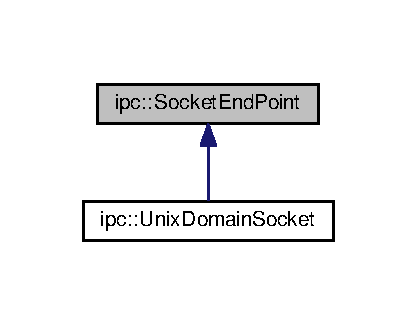
\includegraphics[width=200pt]{classipc_1_1SocketEndPoint__inherit__graph}
\end{center}
\end{figure}
\subsection*{Public Member Functions}
\begin{DoxyCompactItemize}
\item 
\hyperlink{classipc_1_1SocketEndPoint_a24700cf1faa9804dd9959ce1f25bd1b4}{Socket\+End\+Point} ()
\item 
virtual \hyperlink{classipc_1_1SocketEndPoint_a9c99d24a44f871ce8a69b5220e381855}{$\sim$\+Socket\+End\+Point} ()
\item 
virtual int \hyperlink{classipc_1_1SocketEndPoint_a84ded69d1b4d517aaefceeee03fe0846}{initialize\+Socket} ()=0
\item 
virtual bool \hyperlink{classipc_1_1SocketEndPoint_a81b916a8e92b383afa9d0bb85a76e364}{connect\+To\+Server} ()=0
\item 
virtual bool \hyperlink{classipc_1_1SocketEndPoint_a6de9aa716acefb344ddc566df4c1628d}{bind\+Socket} ()=0
\item 
virtual bool \hyperlink{classipc_1_1SocketEndPoint_a4e1ada6c59c1fc4b8d2a75e5939f06e5}{listen\+Socket} ()=0
\item 
virtual int \hyperlink{classipc_1_1SocketEndPoint_ab025dab15878d325d0932f0b813e31f4}{accept\+Request} ()=0
\item 
virtual Emp\+Full\+Message $\ast$ \hyperlink{classipc_1_1SocketEndPoint_ac626b7166cdda6bc1434d897c335e6b8}{read\+Data} ()=0
\item 
virtual void \hyperlink{classipc_1_1SocketEndPoint_ad487a279c5f3456e241a71f4b37173a1}{write\+Data} (Emp\+Full\+Message $\ast$message)=0
\item 
virtual void \hyperlink{classipc_1_1SocketEndPoint_adacb2194fa63c2eff027c094b4958997}{set\+Non\+Blocking} (int socket\+FD)=0
\item 
virtual void \hyperlink{classipc_1_1SocketEndPoint_a65dba66f56f769ae7b424cb40dd2cf5b}{destroy} ()=0
\item 
virtual bool \hyperlink{classipc_1_1SocketEndPoint_a3c86a15ac04aa3fe9480b4f6c7b09ae3}{get\+Current\+State} ()=0
\end{DoxyCompactItemize}
\subsection*{Static Public Member Functions}
\begin{DoxyCompactItemize}
\item 
static void \hyperlink{classipc_1_1SocketEndPoint_a637ace8f8872aa88463405ac95561578}{init\+Config\+Items} (string sz\+File\+Name)
\end{DoxyCompactItemize}


\subsection{Detailed Description}


Definition at line 21 of file Socket\+End\+Point.\+h.



\subsection{Constructor \& Destructor Documentation}
\index{ipc\+::\+Socket\+End\+Point@{ipc\+::\+Socket\+End\+Point}!Socket\+End\+Point@{Socket\+End\+Point}}
\index{Socket\+End\+Point@{Socket\+End\+Point}!ipc\+::\+Socket\+End\+Point@{ipc\+::\+Socket\+End\+Point}}
\subsubsection[{\texorpdfstring{Socket\+End\+Point()}{SocketEndPoint()}}]{\setlength{\rightskip}{0pt plus 5cm}Socket\+End\+Point\+::\+Socket\+End\+Point (
\begin{DoxyParamCaption}
{}
\end{DoxyParamCaption}
)}\hypertarget{classipc_1_1SocketEndPoint_a24700cf1faa9804dd9959ce1f25bd1b4}{}\label{classipc_1_1SocketEndPoint_a24700cf1faa9804dd9959ce1f25bd1b4}


Definition at line 14 of file Socket\+End\+Point.\+cpp.

\index{ipc\+::\+Socket\+End\+Point@{ipc\+::\+Socket\+End\+Point}!````~Socket\+End\+Point@{$\sim$\+Socket\+End\+Point}}
\index{````~Socket\+End\+Point@{$\sim$\+Socket\+End\+Point}!ipc\+::\+Socket\+End\+Point@{ipc\+::\+Socket\+End\+Point}}
\subsubsection[{\texorpdfstring{$\sim$\+Socket\+End\+Point()}{~SocketEndPoint()}}]{\setlength{\rightskip}{0pt plus 5cm}Socket\+End\+Point\+::$\sim$\+Socket\+End\+Point (
\begin{DoxyParamCaption}
{}
\end{DoxyParamCaption}
)\hspace{0.3cm}{\ttfamily [virtual]}}\hypertarget{classipc_1_1SocketEndPoint_a9c99d24a44f871ce8a69b5220e381855}{}\label{classipc_1_1SocketEndPoint_a9c99d24a44f871ce8a69b5220e381855}


Definition at line 18 of file Socket\+End\+Point.\+cpp.



\subsection{Member Function Documentation}
\index{ipc\+::\+Socket\+End\+Point@{ipc\+::\+Socket\+End\+Point}!accept\+Request@{accept\+Request}}
\index{accept\+Request@{accept\+Request}!ipc\+::\+Socket\+End\+Point@{ipc\+::\+Socket\+End\+Point}}
\subsubsection[{\texorpdfstring{accept\+Request()=0}{acceptRequest()=0}}]{\setlength{\rightskip}{0pt plus 5cm}virtual int ipc\+::\+Socket\+End\+Point\+::accept\+Request (
\begin{DoxyParamCaption}
{}
\end{DoxyParamCaption}
)\hspace{0.3cm}{\ttfamily [pure virtual]}}\hypertarget{classipc_1_1SocketEndPoint_ab025dab15878d325d0932f0b813e31f4}{}\label{classipc_1_1SocketEndPoint_ab025dab15878d325d0932f0b813e31f4}


Implemented in \hyperlink{classipc_1_1UnixDomainSocket_a381d1f377da1a980bddfde2abb577bf0}{ipc\+::\+Unix\+Domain\+Socket}.



Here is the caller graph for this function\+:
\nopagebreak
\begin{figure}[H]
\begin{center}
\leavevmode
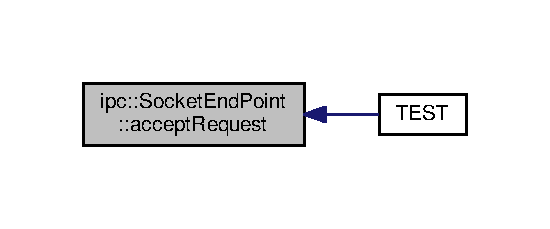
\includegraphics[width=264pt]{classipc_1_1SocketEndPoint_ab025dab15878d325d0932f0b813e31f4_icgraph}
\end{center}
\end{figure}


\index{ipc\+::\+Socket\+End\+Point@{ipc\+::\+Socket\+End\+Point}!bind\+Socket@{bind\+Socket}}
\index{bind\+Socket@{bind\+Socket}!ipc\+::\+Socket\+End\+Point@{ipc\+::\+Socket\+End\+Point}}
\subsubsection[{\texorpdfstring{bind\+Socket()=0}{bindSocket()=0}}]{\setlength{\rightskip}{0pt plus 5cm}virtual bool ipc\+::\+Socket\+End\+Point\+::bind\+Socket (
\begin{DoxyParamCaption}
{}
\end{DoxyParamCaption}
)\hspace{0.3cm}{\ttfamily [pure virtual]}}\hypertarget{classipc_1_1SocketEndPoint_a6de9aa716acefb344ddc566df4c1628d}{}\label{classipc_1_1SocketEndPoint_a6de9aa716acefb344ddc566df4c1628d}


Implemented in \hyperlink{classipc_1_1UnixDomainSocket_a5dddd0aef5c2184843f573c19156ba37}{ipc\+::\+Unix\+Domain\+Socket}.



Here is the caller graph for this function\+:
\nopagebreak
\begin{figure}[H]
\begin{center}
\leavevmode
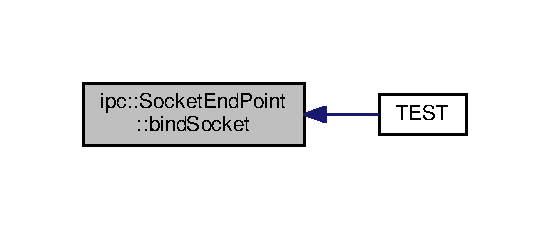
\includegraphics[width=264pt]{classipc_1_1SocketEndPoint_a6de9aa716acefb344ddc566df4c1628d_icgraph}
\end{center}
\end{figure}


\index{ipc\+::\+Socket\+End\+Point@{ipc\+::\+Socket\+End\+Point}!connect\+To\+Server@{connect\+To\+Server}}
\index{connect\+To\+Server@{connect\+To\+Server}!ipc\+::\+Socket\+End\+Point@{ipc\+::\+Socket\+End\+Point}}
\subsubsection[{\texorpdfstring{connect\+To\+Server()=0}{connectToServer()=0}}]{\setlength{\rightskip}{0pt plus 5cm}virtual bool ipc\+::\+Socket\+End\+Point\+::connect\+To\+Server (
\begin{DoxyParamCaption}
{}
\end{DoxyParamCaption}
)\hspace{0.3cm}{\ttfamily [pure virtual]}}\hypertarget{classipc_1_1SocketEndPoint_a81b916a8e92b383afa9d0bb85a76e364}{}\label{classipc_1_1SocketEndPoint_a81b916a8e92b383afa9d0bb85a76e364}


Implemented in \hyperlink{classipc_1_1UnixDomainSocket_acaf4e80b5d2e0069c0347cb7ad69b279}{ipc\+::\+Unix\+Domain\+Socket}.



Here is the caller graph for this function\+:
\nopagebreak
\begin{figure}[H]
\begin{center}
\leavevmode
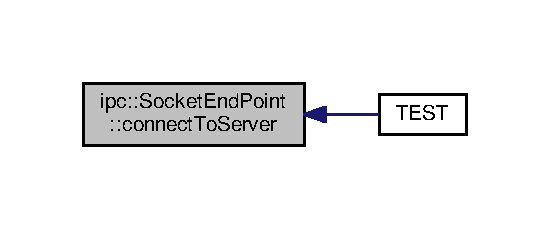
\includegraphics[width=264pt]{classipc_1_1SocketEndPoint_a81b916a8e92b383afa9d0bb85a76e364_icgraph}
\end{center}
\end{figure}


\index{ipc\+::\+Socket\+End\+Point@{ipc\+::\+Socket\+End\+Point}!destroy@{destroy}}
\index{destroy@{destroy}!ipc\+::\+Socket\+End\+Point@{ipc\+::\+Socket\+End\+Point}}
\subsubsection[{\texorpdfstring{destroy()=0}{destroy()=0}}]{\setlength{\rightskip}{0pt plus 5cm}virtual void ipc\+::\+Socket\+End\+Point\+::destroy (
\begin{DoxyParamCaption}
{}
\end{DoxyParamCaption}
)\hspace{0.3cm}{\ttfamily [pure virtual]}}\hypertarget{classipc_1_1SocketEndPoint_a65dba66f56f769ae7b424cb40dd2cf5b}{}\label{classipc_1_1SocketEndPoint_a65dba66f56f769ae7b424cb40dd2cf5b}


Implemented in \hyperlink{classipc_1_1UnixDomainSocket_ae8e7915608903f74300a9f626bdb3d3f}{ipc\+::\+Unix\+Domain\+Socket}.



Here is the caller graph for this function\+:
\nopagebreak
\begin{figure}[H]
\begin{center}
\leavevmode
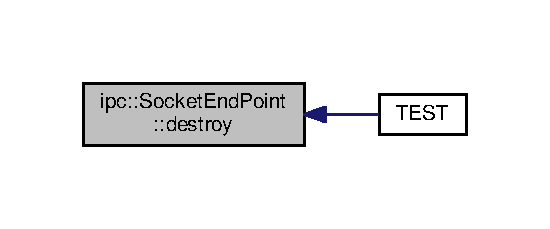
\includegraphics[width=264pt]{classipc_1_1SocketEndPoint_a65dba66f56f769ae7b424cb40dd2cf5b_icgraph}
\end{center}
\end{figure}


\index{ipc\+::\+Socket\+End\+Point@{ipc\+::\+Socket\+End\+Point}!get\+Current\+State@{get\+Current\+State}}
\index{get\+Current\+State@{get\+Current\+State}!ipc\+::\+Socket\+End\+Point@{ipc\+::\+Socket\+End\+Point}}
\subsubsection[{\texorpdfstring{get\+Current\+State()=0}{getCurrentState()=0}}]{\setlength{\rightskip}{0pt plus 5cm}virtual bool ipc\+::\+Socket\+End\+Point\+::get\+Current\+State (
\begin{DoxyParamCaption}
{}
\end{DoxyParamCaption}
)\hspace{0.3cm}{\ttfamily [pure virtual]}}\hypertarget{classipc_1_1SocketEndPoint_a3c86a15ac04aa3fe9480b4f6c7b09ae3}{}\label{classipc_1_1SocketEndPoint_a3c86a15ac04aa3fe9480b4f6c7b09ae3}


Implemented in \hyperlink{classipc_1_1UnixDomainSocket_a7fc2dceda50345568051d849c1c396dd}{ipc\+::\+Unix\+Domain\+Socket}.

\index{ipc\+::\+Socket\+End\+Point@{ipc\+::\+Socket\+End\+Point}!init\+Config\+Items@{init\+Config\+Items}}
\index{init\+Config\+Items@{init\+Config\+Items}!ipc\+::\+Socket\+End\+Point@{ipc\+::\+Socket\+End\+Point}}
\subsubsection[{\texorpdfstring{init\+Config\+Items(string sz\+File\+Name)}{initConfigItems(string szFileName)}}]{\setlength{\rightskip}{0pt plus 5cm}static void ipc\+::\+Socket\+End\+Point\+::init\+Config\+Items (
\begin{DoxyParamCaption}
\item[{string}]{sz\+File\+Name}
\end{DoxyParamCaption}
)\hspace{0.3cm}{\ttfamily [static]}}\hypertarget{classipc_1_1SocketEndPoint_a637ace8f8872aa88463405ac95561578}{}\label{classipc_1_1SocketEndPoint_a637ace8f8872aa88463405ac95561578}
\index{ipc\+::\+Socket\+End\+Point@{ipc\+::\+Socket\+End\+Point}!initialize\+Socket@{initialize\+Socket}}
\index{initialize\+Socket@{initialize\+Socket}!ipc\+::\+Socket\+End\+Point@{ipc\+::\+Socket\+End\+Point}}
\subsubsection[{\texorpdfstring{initialize\+Socket()=0}{initializeSocket()=0}}]{\setlength{\rightskip}{0pt plus 5cm}virtual int ipc\+::\+Socket\+End\+Point\+::initialize\+Socket (
\begin{DoxyParamCaption}
{}
\end{DoxyParamCaption}
)\hspace{0.3cm}{\ttfamily [pure virtual]}}\hypertarget{classipc_1_1SocketEndPoint_a84ded69d1b4d517aaefceeee03fe0846}{}\label{classipc_1_1SocketEndPoint_a84ded69d1b4d517aaefceeee03fe0846}


Implemented in \hyperlink{classipc_1_1UnixDomainSocket_ae1d8cecdd27269a77969b128e2f70774}{ipc\+::\+Unix\+Domain\+Socket}.



Here is the caller graph for this function\+:
\nopagebreak
\begin{figure}[H]
\begin{center}
\leavevmode
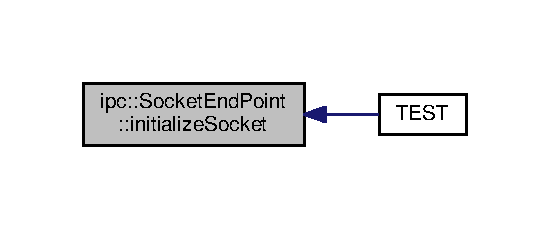
\includegraphics[width=264pt]{classipc_1_1SocketEndPoint_a84ded69d1b4d517aaefceeee03fe0846_icgraph}
\end{center}
\end{figure}


\index{ipc\+::\+Socket\+End\+Point@{ipc\+::\+Socket\+End\+Point}!listen\+Socket@{listen\+Socket}}
\index{listen\+Socket@{listen\+Socket}!ipc\+::\+Socket\+End\+Point@{ipc\+::\+Socket\+End\+Point}}
\subsubsection[{\texorpdfstring{listen\+Socket()=0}{listenSocket()=0}}]{\setlength{\rightskip}{0pt plus 5cm}virtual bool ipc\+::\+Socket\+End\+Point\+::listen\+Socket (
\begin{DoxyParamCaption}
{}
\end{DoxyParamCaption}
)\hspace{0.3cm}{\ttfamily [pure virtual]}}\hypertarget{classipc_1_1SocketEndPoint_a4e1ada6c59c1fc4b8d2a75e5939f06e5}{}\label{classipc_1_1SocketEndPoint_a4e1ada6c59c1fc4b8d2a75e5939f06e5}


Implemented in \hyperlink{classipc_1_1UnixDomainSocket_a2887b754b2b26b7c4c947aa27a8a75c8}{ipc\+::\+Unix\+Domain\+Socket}.



Here is the caller graph for this function\+:
\nopagebreak
\begin{figure}[H]
\begin{center}
\leavevmode
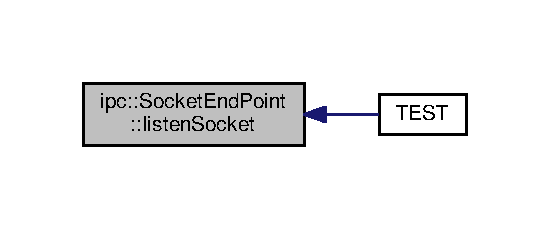
\includegraphics[width=264pt]{classipc_1_1SocketEndPoint_a4e1ada6c59c1fc4b8d2a75e5939f06e5_icgraph}
\end{center}
\end{figure}


\index{ipc\+::\+Socket\+End\+Point@{ipc\+::\+Socket\+End\+Point}!read\+Data@{read\+Data}}
\index{read\+Data@{read\+Data}!ipc\+::\+Socket\+End\+Point@{ipc\+::\+Socket\+End\+Point}}
\subsubsection[{\texorpdfstring{read\+Data()=0}{readData()=0}}]{\setlength{\rightskip}{0pt plus 5cm}virtual Emp\+Full\+Message$\ast$ ipc\+::\+Socket\+End\+Point\+::read\+Data (
\begin{DoxyParamCaption}
{}
\end{DoxyParamCaption}
)\hspace{0.3cm}{\ttfamily [pure virtual]}}\hypertarget{classipc_1_1SocketEndPoint_ac626b7166cdda6bc1434d897c335e6b8}{}\label{classipc_1_1SocketEndPoint_ac626b7166cdda6bc1434d897c335e6b8}


Implemented in \hyperlink{classipc_1_1UnixDomainSocket_a694233d63430495b4ecbc5c5b59c01e4}{ipc\+::\+Unix\+Domain\+Socket}.



Here is the caller graph for this function\+:
\nopagebreak
\begin{figure}[H]
\begin{center}
\leavevmode
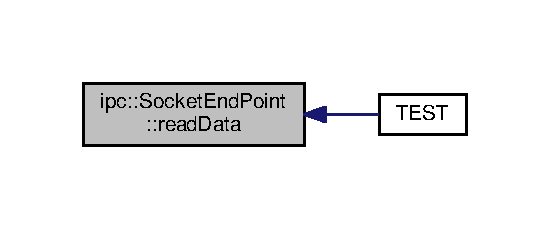
\includegraphics[width=264pt]{classipc_1_1SocketEndPoint_ac626b7166cdda6bc1434d897c335e6b8_icgraph}
\end{center}
\end{figure}


\index{ipc\+::\+Socket\+End\+Point@{ipc\+::\+Socket\+End\+Point}!set\+Non\+Blocking@{set\+Non\+Blocking}}
\index{set\+Non\+Blocking@{set\+Non\+Blocking}!ipc\+::\+Socket\+End\+Point@{ipc\+::\+Socket\+End\+Point}}
\subsubsection[{\texorpdfstring{set\+Non\+Blocking(int socket\+F\+D)=0}{setNonBlocking(int socketFD)=0}}]{\setlength{\rightskip}{0pt plus 5cm}virtual void ipc\+::\+Socket\+End\+Point\+::set\+Non\+Blocking (
\begin{DoxyParamCaption}
\item[{int}]{socket\+FD}
\end{DoxyParamCaption}
)\hspace{0.3cm}{\ttfamily [pure virtual]}}\hypertarget{classipc_1_1SocketEndPoint_adacb2194fa63c2eff027c094b4958997}{}\label{classipc_1_1SocketEndPoint_adacb2194fa63c2eff027c094b4958997}


Implemented in \hyperlink{classipc_1_1UnixDomainSocket_abbb0ec8d20157b203eee0eabcda81ec9}{ipc\+::\+Unix\+Domain\+Socket}.



Here is the caller graph for this function\+:
\nopagebreak
\begin{figure}[H]
\begin{center}
\leavevmode
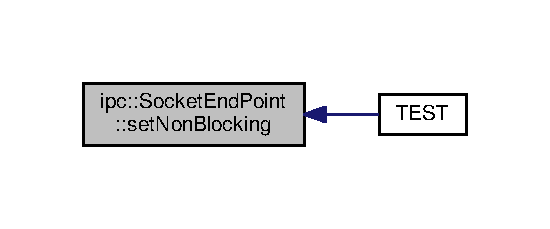
\includegraphics[width=264pt]{classipc_1_1SocketEndPoint_adacb2194fa63c2eff027c094b4958997_icgraph}
\end{center}
\end{figure}


\index{ipc\+::\+Socket\+End\+Point@{ipc\+::\+Socket\+End\+Point}!write\+Data@{write\+Data}}
\index{write\+Data@{write\+Data}!ipc\+::\+Socket\+End\+Point@{ipc\+::\+Socket\+End\+Point}}
\subsubsection[{\texorpdfstring{write\+Data(\+Emp\+Full\+Message $\ast$message)=0}{writeData(EmpFullMessage *message)=0}}]{\setlength{\rightskip}{0pt plus 5cm}virtual void ipc\+::\+Socket\+End\+Point\+::write\+Data (
\begin{DoxyParamCaption}
\item[{Emp\+Full\+Message $\ast$}]{message}
\end{DoxyParamCaption}
)\hspace{0.3cm}{\ttfamily [pure virtual]}}\hypertarget{classipc_1_1SocketEndPoint_ad487a279c5f3456e241a71f4b37173a1}{}\label{classipc_1_1SocketEndPoint_ad487a279c5f3456e241a71f4b37173a1}


Implemented in \hyperlink{classipc_1_1UnixDomainSocket_aff0368529a5eebb701e4689213880a97}{ipc\+::\+Unix\+Domain\+Socket}.



Here is the caller graph for this function\+:
\nopagebreak
\begin{figure}[H]
\begin{center}
\leavevmode
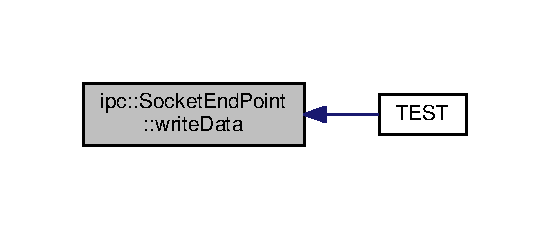
\includegraphics[width=264pt]{classipc_1_1SocketEndPoint_ad487a279c5f3456e241a71f4b37173a1_icgraph}
\end{center}
\end{figure}




The documentation for this class was generated from the following files\+:\begin{DoxyCompactItemize}
\item 
C\+O\+M\+M\+O\+N/\hyperlink{SocketEndPoint_8h}{Socket\+End\+Point.\+h}\item 
C\+O\+M\+M\+O\+N/\hyperlink{SocketEndPoint_8cpp}{Socket\+End\+Point.\+cpp}\end{DoxyCompactItemize}

\hypertarget{classipc_1_1UnixDomainSocket}{}\section{ipc\+:\+:Unix\+Domain\+Socket Class Reference}
\label{classipc_1_1UnixDomainSocket}\index{ipc\+::\+Unix\+Domain\+Socket@{ipc\+::\+Unix\+Domain\+Socket}}


{\ttfamily \#include $<$Unix\+Domain\+Socket.\+h$>$}



Inheritance diagram for ipc\+:\+:Unix\+Domain\+Socket\+:
\nopagebreak
\begin{figure}[H]
\begin{center}
\leavevmode
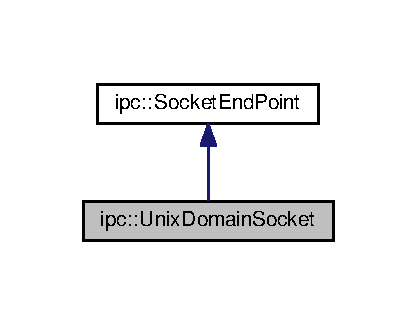
\includegraphics[width=200pt]{classipc_1_1UnixDomainSocket__inherit__graph}
\end{center}
\end{figure}


Collaboration diagram for ipc\+:\+:Unix\+Domain\+Socket\+:
\nopagebreak
\begin{figure}[H]
\begin{center}
\leavevmode
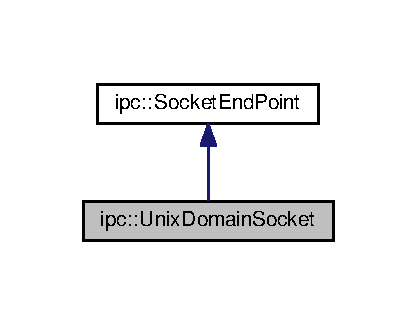
\includegraphics[width=200pt]{classipc_1_1UnixDomainSocket__coll__graph}
\end{center}
\end{figure}
\subsection*{Public Member Functions}
\begin{DoxyCompactItemize}
\item 
\hyperlink{classipc_1_1UnixDomainSocket_a9d87b6cfaa62cf9fa8d64ed533001753}{Unix\+Domain\+Socket} ()
\item 
\hyperlink{classipc_1_1UnixDomainSocket_a10ab8e00efe147e7f313a1298113244a}{Unix\+Domain\+Socket} (\hyperlink{classipc_1_1EndPoint_adcdf30d3a61d3d342529b1fb8b0bbd72}{End\+Point\+::\+Protocol\+Type} protocol\+Type)
\item 
virtual \hyperlink{classipc_1_1UnixDomainSocket_a77a7af339ff0c934d90586d124244e7b}{$\sim$\+Unix\+Domain\+Socket} ()
\item 
Emp\+Full\+Message $\ast$ \hyperlink{classipc_1_1UnixDomainSocket_a694233d63430495b4ecbc5c5b59c01e4}{read\+Data} ()
\item 
void \hyperlink{classipc_1_1UnixDomainSocket_aff0368529a5eebb701e4689213880a97}{write\+Data} (Emp\+Full\+Message $\ast$message)
\item 
void \hyperlink{classipc_1_1UnixDomainSocket_ae8e7915608903f74300a9f626bdb3d3f}{destroy} ()
\item 
int \hyperlink{classipc_1_1UnixDomainSocket_ae1d8cecdd27269a77969b128e2f70774}{initialize\+Socket} ()
\item 
bool \hyperlink{classipc_1_1UnixDomainSocket_acaf4e80b5d2e0069c0347cb7ad69b279}{connect\+To\+Server} ()
\item 
bool \hyperlink{classipc_1_1UnixDomainSocket_a5dddd0aef5c2184843f573c19156ba37}{bind\+Socket} ()
\item 
int \hyperlink{classipc_1_1UnixDomainSocket_a381d1f377da1a980bddfde2abb577bf0}{accept\+Request} ()
\item 
bool \hyperlink{classipc_1_1UnixDomainSocket_a2887b754b2b26b7c4c947aa27a8a75c8}{listen\+Socket} ()
\item 
void \hyperlink{classipc_1_1UnixDomainSocket_abbb0ec8d20157b203eee0eabcda81ec9}{set\+Non\+Blocking} (int socket\+FD)
\item 
bool \hyperlink{classipc_1_1UnixDomainSocket_a7fc2dceda50345568051d849c1c396dd}{get\+Current\+State} ()
\item 
ssize\+\_\+t \hyperlink{classipc_1_1UnixDomainSocket_aa3495bc1d20aaf30d80c14b3fb85f35c}{read\+From\+FD} (int fd, boost\+::uint8\+\_\+t $\ast$buffer, size\+\_\+t size)
\end{DoxyCompactItemize}
\subsection*{Public Attributes}
\begin{DoxyCompactItemize}
\item 
size\+\_\+t \hyperlink{classipc_1_1UnixDomainSocket_a2a7e269ee896e8ca6fc4400c28d22f46}{m\+\_\+total\+Bytes\+Read}
\item 
size\+\_\+t \hyperlink{classipc_1_1UnixDomainSocket_a93a554cd7a8c2ef97e22a4e5a28f2191}{m\+\_\+bytes\+Allocated}
\item 
size\+\_\+t \hyperlink{classipc_1_1UnixDomainSocket_a232d748cd70ad72d18d746a9b8ccf537}{m\+\_\+buffer\+Size}
\end{DoxyCompactItemize}
\subsection*{Additional Inherited Members}


\subsection{Detailed Description}


Definition at line 26 of file Unix\+Domain\+Socket.\+h.



\subsection{Constructor \& Destructor Documentation}
\index{ipc\+::\+Unix\+Domain\+Socket@{ipc\+::\+Unix\+Domain\+Socket}!Unix\+Domain\+Socket@{Unix\+Domain\+Socket}}
\index{Unix\+Domain\+Socket@{Unix\+Domain\+Socket}!ipc\+::\+Unix\+Domain\+Socket@{ipc\+::\+Unix\+Domain\+Socket}}
\subsubsection[{\texorpdfstring{Unix\+Domain\+Socket()}{UnixDomainSocket()}}]{\setlength{\rightskip}{0pt plus 5cm}Unix\+Domain\+Socket\+::\+Unix\+Domain\+Socket (
\begin{DoxyParamCaption}
{}
\end{DoxyParamCaption}
)}\hypertarget{classipc_1_1UnixDomainSocket_a9d87b6cfaa62cf9fa8d64ed533001753}{}\label{classipc_1_1UnixDomainSocket_a9d87b6cfaa62cf9fa8d64ed533001753}


Definition at line 25 of file Unix\+Domain\+Socket.\+cpp.

\index{ipc\+::\+Unix\+Domain\+Socket@{ipc\+::\+Unix\+Domain\+Socket}!Unix\+Domain\+Socket@{Unix\+Domain\+Socket}}
\index{Unix\+Domain\+Socket@{Unix\+Domain\+Socket}!ipc\+::\+Unix\+Domain\+Socket@{ipc\+::\+Unix\+Domain\+Socket}}
\subsubsection[{\texorpdfstring{Unix\+Domain\+Socket(\+End\+Point\+::\+Protocol\+Type protocol\+Type)}{UnixDomainSocket(EndPoint::ProtocolType protocolType)}}]{\setlength{\rightskip}{0pt plus 5cm}Unix\+Domain\+Socket\+::\+Unix\+Domain\+Socket (
\begin{DoxyParamCaption}
\item[{{\bf End\+Point\+::\+Protocol\+Type}}]{protocol\+Type}
\end{DoxyParamCaption}
)}\hypertarget{classipc_1_1UnixDomainSocket_a10ab8e00efe147e7f313a1298113244a}{}\label{classipc_1_1UnixDomainSocket_a10ab8e00efe147e7f313a1298113244a}


Definition at line 31 of file Unix\+Domain\+Socket.\+cpp.

\index{ipc\+::\+Unix\+Domain\+Socket@{ipc\+::\+Unix\+Domain\+Socket}!````~Unix\+Domain\+Socket@{$\sim$\+Unix\+Domain\+Socket}}
\index{````~Unix\+Domain\+Socket@{$\sim$\+Unix\+Domain\+Socket}!ipc\+::\+Unix\+Domain\+Socket@{ipc\+::\+Unix\+Domain\+Socket}}
\subsubsection[{\texorpdfstring{$\sim$\+Unix\+Domain\+Socket()}{~UnixDomainSocket()}}]{\setlength{\rightskip}{0pt plus 5cm}Unix\+Domain\+Socket\+::$\sim$\+Unix\+Domain\+Socket (
\begin{DoxyParamCaption}
{}
\end{DoxyParamCaption}
)\hspace{0.3cm}{\ttfamily [virtual]}}\hypertarget{classipc_1_1UnixDomainSocket_a77a7af339ff0c934d90586d124244e7b}{}\label{classipc_1_1UnixDomainSocket_a77a7af339ff0c934d90586d124244e7b}


Definition at line 51 of file Unix\+Domain\+Socket.\+cpp.



\subsection{Member Function Documentation}
\index{ipc\+::\+Unix\+Domain\+Socket@{ipc\+::\+Unix\+Domain\+Socket}!accept\+Request@{accept\+Request}}
\index{accept\+Request@{accept\+Request}!ipc\+::\+Unix\+Domain\+Socket@{ipc\+::\+Unix\+Domain\+Socket}}
\subsubsection[{\texorpdfstring{accept\+Request()}{acceptRequest()}}]{\setlength{\rightskip}{0pt plus 5cm}int Unix\+Domain\+Socket\+::accept\+Request (
\begin{DoxyParamCaption}
{}
\end{DoxyParamCaption}
)\hspace{0.3cm}{\ttfamily [virtual]}}\hypertarget{classipc_1_1UnixDomainSocket_a381d1f377da1a980bddfde2abb577bf0}{}\label{classipc_1_1UnixDomainSocket_a381d1f377da1a980bddfde2abb577bf0}


Implements \hyperlink{classipc_1_1SocketEndPoint_ab025dab15878d325d0932f0b813e31f4}{ipc\+::\+Socket\+End\+Point}.



Definition at line 146 of file Unix\+Domain\+Socket.\+cpp.

\index{ipc\+::\+Unix\+Domain\+Socket@{ipc\+::\+Unix\+Domain\+Socket}!bind\+Socket@{bind\+Socket}}
\index{bind\+Socket@{bind\+Socket}!ipc\+::\+Unix\+Domain\+Socket@{ipc\+::\+Unix\+Domain\+Socket}}
\subsubsection[{\texorpdfstring{bind\+Socket()}{bindSocket()}}]{\setlength{\rightskip}{0pt plus 5cm}bool Unix\+Domain\+Socket\+::bind\+Socket (
\begin{DoxyParamCaption}
{}
\end{DoxyParamCaption}
)\hspace{0.3cm}{\ttfamily [virtual]}}\hypertarget{classipc_1_1UnixDomainSocket_a5dddd0aef5c2184843f573c19156ba37}{}\label{classipc_1_1UnixDomainSocket_a5dddd0aef5c2184843f573c19156ba37}


Implements \hyperlink{classipc_1_1SocketEndPoint_a6de9aa716acefb344ddc566df4c1628d}{ipc\+::\+Socket\+End\+Point}.



Definition at line 128 of file Unix\+Domain\+Socket.\+cpp.

\index{ipc\+::\+Unix\+Domain\+Socket@{ipc\+::\+Unix\+Domain\+Socket}!connect\+To\+Server@{connect\+To\+Server}}
\index{connect\+To\+Server@{connect\+To\+Server}!ipc\+::\+Unix\+Domain\+Socket@{ipc\+::\+Unix\+Domain\+Socket}}
\subsubsection[{\texorpdfstring{connect\+To\+Server()}{connectToServer()}}]{\setlength{\rightskip}{0pt plus 5cm}bool Unix\+Domain\+Socket\+::connect\+To\+Server (
\begin{DoxyParamCaption}
{}
\end{DoxyParamCaption}
)\hspace{0.3cm}{\ttfamily [virtual]}}\hypertarget{classipc_1_1UnixDomainSocket_acaf4e80b5d2e0069c0347cb7ad69b279}{}\label{classipc_1_1UnixDomainSocket_acaf4e80b5d2e0069c0347cb7ad69b279}


Implements \hyperlink{classipc_1_1SocketEndPoint_a81b916a8e92b383afa9d0bb85a76e364}{ipc\+::\+Socket\+End\+Point}.



Definition at line 112 of file Unix\+Domain\+Socket.\+cpp.

\index{ipc\+::\+Unix\+Domain\+Socket@{ipc\+::\+Unix\+Domain\+Socket}!destroy@{destroy}}
\index{destroy@{destroy}!ipc\+::\+Unix\+Domain\+Socket@{ipc\+::\+Unix\+Domain\+Socket}}
\subsubsection[{\texorpdfstring{destroy()}{destroy()}}]{\setlength{\rightskip}{0pt plus 5cm}void Unix\+Domain\+Socket\+::destroy (
\begin{DoxyParamCaption}
{}
\end{DoxyParamCaption}
)\hspace{0.3cm}{\ttfamily [virtual]}}\hypertarget{classipc_1_1UnixDomainSocket_ae8e7915608903f74300a9f626bdb3d3f}{}\label{classipc_1_1UnixDomainSocket_ae8e7915608903f74300a9f626bdb3d3f}


Implements \hyperlink{classipc_1_1SocketEndPoint_a65dba66f56f769ae7b424cb40dd2cf5b}{ipc\+::\+Socket\+End\+Point}.



Definition at line 346 of file Unix\+Domain\+Socket.\+cpp.

\index{ipc\+::\+Unix\+Domain\+Socket@{ipc\+::\+Unix\+Domain\+Socket}!get\+Current\+State@{get\+Current\+State}}
\index{get\+Current\+State@{get\+Current\+State}!ipc\+::\+Unix\+Domain\+Socket@{ipc\+::\+Unix\+Domain\+Socket}}
\subsubsection[{\texorpdfstring{get\+Current\+State()}{getCurrentState()}}]{\setlength{\rightskip}{0pt plus 5cm}bool Unix\+Domain\+Socket\+::get\+Current\+State (
\begin{DoxyParamCaption}
{}
\end{DoxyParamCaption}
)\hspace{0.3cm}{\ttfamily [virtual]}}\hypertarget{classipc_1_1UnixDomainSocket_a7fc2dceda50345568051d849c1c396dd}{}\label{classipc_1_1UnixDomainSocket_a7fc2dceda50345568051d849c1c396dd}


Implements \hyperlink{classipc_1_1SocketEndPoint_a3c86a15ac04aa3fe9480b4f6c7b09ae3}{ipc\+::\+Socket\+End\+Point}.



Definition at line 353 of file Unix\+Domain\+Socket.\+cpp.

\index{ipc\+::\+Unix\+Domain\+Socket@{ipc\+::\+Unix\+Domain\+Socket}!initialize\+Socket@{initialize\+Socket}}
\index{initialize\+Socket@{initialize\+Socket}!ipc\+::\+Unix\+Domain\+Socket@{ipc\+::\+Unix\+Domain\+Socket}}
\subsubsection[{\texorpdfstring{initialize\+Socket()}{initializeSocket()}}]{\setlength{\rightskip}{0pt plus 5cm}int Unix\+Domain\+Socket\+::initialize\+Socket (
\begin{DoxyParamCaption}
{}
\end{DoxyParamCaption}
)\hspace{0.3cm}{\ttfamily [virtual]}}\hypertarget{classipc_1_1UnixDomainSocket_ae1d8cecdd27269a77969b128e2f70774}{}\label{classipc_1_1UnixDomainSocket_ae1d8cecdd27269a77969b128e2f70774}


Implements \hyperlink{classipc_1_1SocketEndPoint_a84ded69d1b4d517aaefceeee03fe0846}{ipc\+::\+Socket\+End\+Point}.



Definition at line 63 of file Unix\+Domain\+Socket.\+cpp.

\index{ipc\+::\+Unix\+Domain\+Socket@{ipc\+::\+Unix\+Domain\+Socket}!listen\+Socket@{listen\+Socket}}
\index{listen\+Socket@{listen\+Socket}!ipc\+::\+Unix\+Domain\+Socket@{ipc\+::\+Unix\+Domain\+Socket}}
\subsubsection[{\texorpdfstring{listen\+Socket()}{listenSocket()}}]{\setlength{\rightskip}{0pt plus 5cm}bool Unix\+Domain\+Socket\+::listen\+Socket (
\begin{DoxyParamCaption}
{}
\end{DoxyParamCaption}
)\hspace{0.3cm}{\ttfamily [virtual]}}\hypertarget{classipc_1_1UnixDomainSocket_a2887b754b2b26b7c4c947aa27a8a75c8}{}\label{classipc_1_1UnixDomainSocket_a2887b754b2b26b7c4c947aa27a8a75c8}


Implements \hyperlink{classipc_1_1SocketEndPoint_a4e1ada6c59c1fc4b8d2a75e5939f06e5}{ipc\+::\+Socket\+End\+Point}.



Definition at line 168 of file Unix\+Domain\+Socket.\+cpp.

\index{ipc\+::\+Unix\+Domain\+Socket@{ipc\+::\+Unix\+Domain\+Socket}!read\+Data@{read\+Data}}
\index{read\+Data@{read\+Data}!ipc\+::\+Unix\+Domain\+Socket@{ipc\+::\+Unix\+Domain\+Socket}}
\subsubsection[{\texorpdfstring{read\+Data()}{readData()}}]{\setlength{\rightskip}{0pt plus 5cm}Emp\+Full\+Message $\ast$ Unix\+Domain\+Socket\+::read\+Data (
\begin{DoxyParamCaption}
{}
\end{DoxyParamCaption}
)\hspace{0.3cm}{\ttfamily [virtual]}}\hypertarget{classipc_1_1UnixDomainSocket_a694233d63430495b4ecbc5c5b59c01e4}{}\label{classipc_1_1UnixDomainSocket_a694233d63430495b4ecbc5c5b59c01e4}


Implements \hyperlink{classipc_1_1SocketEndPoint_ac626b7166cdda6bc1434d897c335e6b8}{ipc\+::\+Socket\+End\+Point}.



Definition at line 228 of file Unix\+Domain\+Socket.\+cpp.

\index{ipc\+::\+Unix\+Domain\+Socket@{ipc\+::\+Unix\+Domain\+Socket}!read\+From\+FD@{read\+From\+FD}}
\index{read\+From\+FD@{read\+From\+FD}!ipc\+::\+Unix\+Domain\+Socket@{ipc\+::\+Unix\+Domain\+Socket}}
\subsubsection[{\texorpdfstring{read\+From\+F\+D(int fd, boost\+::uint8\+\_\+t $\ast$buffer, size\+\_\+t size)}{readFromFD(int fd, boost::uint8_t *buffer, size_t size)}}]{\setlength{\rightskip}{0pt plus 5cm}ssize\+\_\+t Unix\+Domain\+Socket\+::read\+From\+FD (
\begin{DoxyParamCaption}
\item[{int}]{fd, }
\item[{boost\+::uint8\+\_\+t $\ast$}]{buffer, }
\item[{size\+\_\+t}]{size}
\end{DoxyParamCaption}
)}\hypertarget{classipc_1_1UnixDomainSocket_aa3495bc1d20aaf30d80c14b3fb85f35c}{}\label{classipc_1_1UnixDomainSocket_aa3495bc1d20aaf30d80c14b3fb85f35c}


Definition at line 197 of file Unix\+Domain\+Socket.\+cpp.

\index{ipc\+::\+Unix\+Domain\+Socket@{ipc\+::\+Unix\+Domain\+Socket}!set\+Non\+Blocking@{set\+Non\+Blocking}}
\index{set\+Non\+Blocking@{set\+Non\+Blocking}!ipc\+::\+Unix\+Domain\+Socket@{ipc\+::\+Unix\+Domain\+Socket}}
\subsubsection[{\texorpdfstring{set\+Non\+Blocking(int socket\+F\+D)}{setNonBlocking(int socketFD)}}]{\setlength{\rightskip}{0pt plus 5cm}void Unix\+Domain\+Socket\+::set\+Non\+Blocking (
\begin{DoxyParamCaption}
\item[{int}]{socket\+FD}
\end{DoxyParamCaption}
)\hspace{0.3cm}{\ttfamily [virtual]}}\hypertarget{classipc_1_1UnixDomainSocket_abbb0ec8d20157b203eee0eabcda81ec9}{}\label{classipc_1_1UnixDomainSocket_abbb0ec8d20157b203eee0eabcda81ec9}


Implements \hyperlink{classipc_1_1SocketEndPoint_adacb2194fa63c2eff027c094b4958997}{ipc\+::\+Socket\+End\+Point}.



Definition at line 192 of file Unix\+Domain\+Socket.\+cpp.

\index{ipc\+::\+Unix\+Domain\+Socket@{ipc\+::\+Unix\+Domain\+Socket}!write\+Data@{write\+Data}}
\index{write\+Data@{write\+Data}!ipc\+::\+Unix\+Domain\+Socket@{ipc\+::\+Unix\+Domain\+Socket}}
\subsubsection[{\texorpdfstring{write\+Data(\+Emp\+Full\+Message $\ast$message)}{writeData(EmpFullMessage *message)}}]{\setlength{\rightskip}{0pt plus 5cm}void Unix\+Domain\+Socket\+::write\+Data (
\begin{DoxyParamCaption}
\item[{Emp\+Full\+Message $\ast$}]{message}
\end{DoxyParamCaption}
)\hspace{0.3cm}{\ttfamily [virtual]}}\hypertarget{classipc_1_1UnixDomainSocket_aff0368529a5eebb701e4689213880a97}{}\label{classipc_1_1UnixDomainSocket_aff0368529a5eebb701e4689213880a97}


Implements \hyperlink{classipc_1_1SocketEndPoint_ad487a279c5f3456e241a71f4b37173a1}{ipc\+::\+Socket\+End\+Point}.



Definition at line 310 of file Unix\+Domain\+Socket.\+cpp.



\subsection{Member Data Documentation}
\index{ipc\+::\+Unix\+Domain\+Socket@{ipc\+::\+Unix\+Domain\+Socket}!m\+\_\+buffer\+Size@{m\+\_\+buffer\+Size}}
\index{m\+\_\+buffer\+Size@{m\+\_\+buffer\+Size}!ipc\+::\+Unix\+Domain\+Socket@{ipc\+::\+Unix\+Domain\+Socket}}
\subsubsection[{\texorpdfstring{m\+\_\+buffer\+Size}{m_bufferSize}}]{\setlength{\rightskip}{0pt plus 5cm}size\+\_\+t ipc\+::\+Unix\+Domain\+Socket\+::m\+\_\+buffer\+Size}\hypertarget{classipc_1_1UnixDomainSocket_a232d748cd70ad72d18d746a9b8ccf537}{}\label{classipc_1_1UnixDomainSocket_a232d748cd70ad72d18d746a9b8ccf537}


Definition at line 129 of file Unix\+Domain\+Socket.\+h.

\index{ipc\+::\+Unix\+Domain\+Socket@{ipc\+::\+Unix\+Domain\+Socket}!m\+\_\+bytes\+Allocated@{m\+\_\+bytes\+Allocated}}
\index{m\+\_\+bytes\+Allocated@{m\+\_\+bytes\+Allocated}!ipc\+::\+Unix\+Domain\+Socket@{ipc\+::\+Unix\+Domain\+Socket}}
\subsubsection[{\texorpdfstring{m\+\_\+bytes\+Allocated}{m_bytesAllocated}}]{\setlength{\rightskip}{0pt plus 5cm}size\+\_\+t ipc\+::\+Unix\+Domain\+Socket\+::m\+\_\+bytes\+Allocated}\hypertarget{classipc_1_1UnixDomainSocket_a93a554cd7a8c2ef97e22a4e5a28f2191}{}\label{classipc_1_1UnixDomainSocket_a93a554cd7a8c2ef97e22a4e5a28f2191}


Definition at line 128 of file Unix\+Domain\+Socket.\+h.

\index{ipc\+::\+Unix\+Domain\+Socket@{ipc\+::\+Unix\+Domain\+Socket}!m\+\_\+total\+Bytes\+Read@{m\+\_\+total\+Bytes\+Read}}
\index{m\+\_\+total\+Bytes\+Read@{m\+\_\+total\+Bytes\+Read}!ipc\+::\+Unix\+Domain\+Socket@{ipc\+::\+Unix\+Domain\+Socket}}
\subsubsection[{\texorpdfstring{m\+\_\+total\+Bytes\+Read}{m_totalBytesRead}}]{\setlength{\rightskip}{0pt plus 5cm}size\+\_\+t ipc\+::\+Unix\+Domain\+Socket\+::m\+\_\+total\+Bytes\+Read}\hypertarget{classipc_1_1UnixDomainSocket_a2a7e269ee896e8ca6fc4400c28d22f46}{}\label{classipc_1_1UnixDomainSocket_a2a7e269ee896e8ca6fc4400c28d22f46}


Definition at line 127 of file Unix\+Domain\+Socket.\+h.



The documentation for this class was generated from the following files\+:\begin{DoxyCompactItemize}
\item 
I\+P\+C\+\_\+\+U\+D\+S/\hyperlink{UnixDomainSocket_8h}{Unix\+Domain\+Socket.\+h}\item 
I\+P\+C\+\_\+\+U\+D\+S/\hyperlink{UnixDomainSocket_8cpp}{Unix\+Domain\+Socket.\+cpp}\end{DoxyCompactItemize}

\chapter{File Documentation}
\hypertarget{EndPoint_8cpp}{}\section{C\+O\+M\+M\+O\+N/\+End\+Point.cpp File Reference}
\label{EndPoint_8cpp}\index{C\+O\+M\+M\+O\+N/\+End\+Point.\+cpp@{C\+O\+M\+M\+O\+N/\+End\+Point.\+cpp}}
{\ttfamily \#include \char`\"{}End\+Point.\+h\char`\"{}}\\*
Include dependency graph for End\+Point.\+cpp\+:
\nopagebreak
\begin{figure}[H]
\begin{center}
\leavevmode
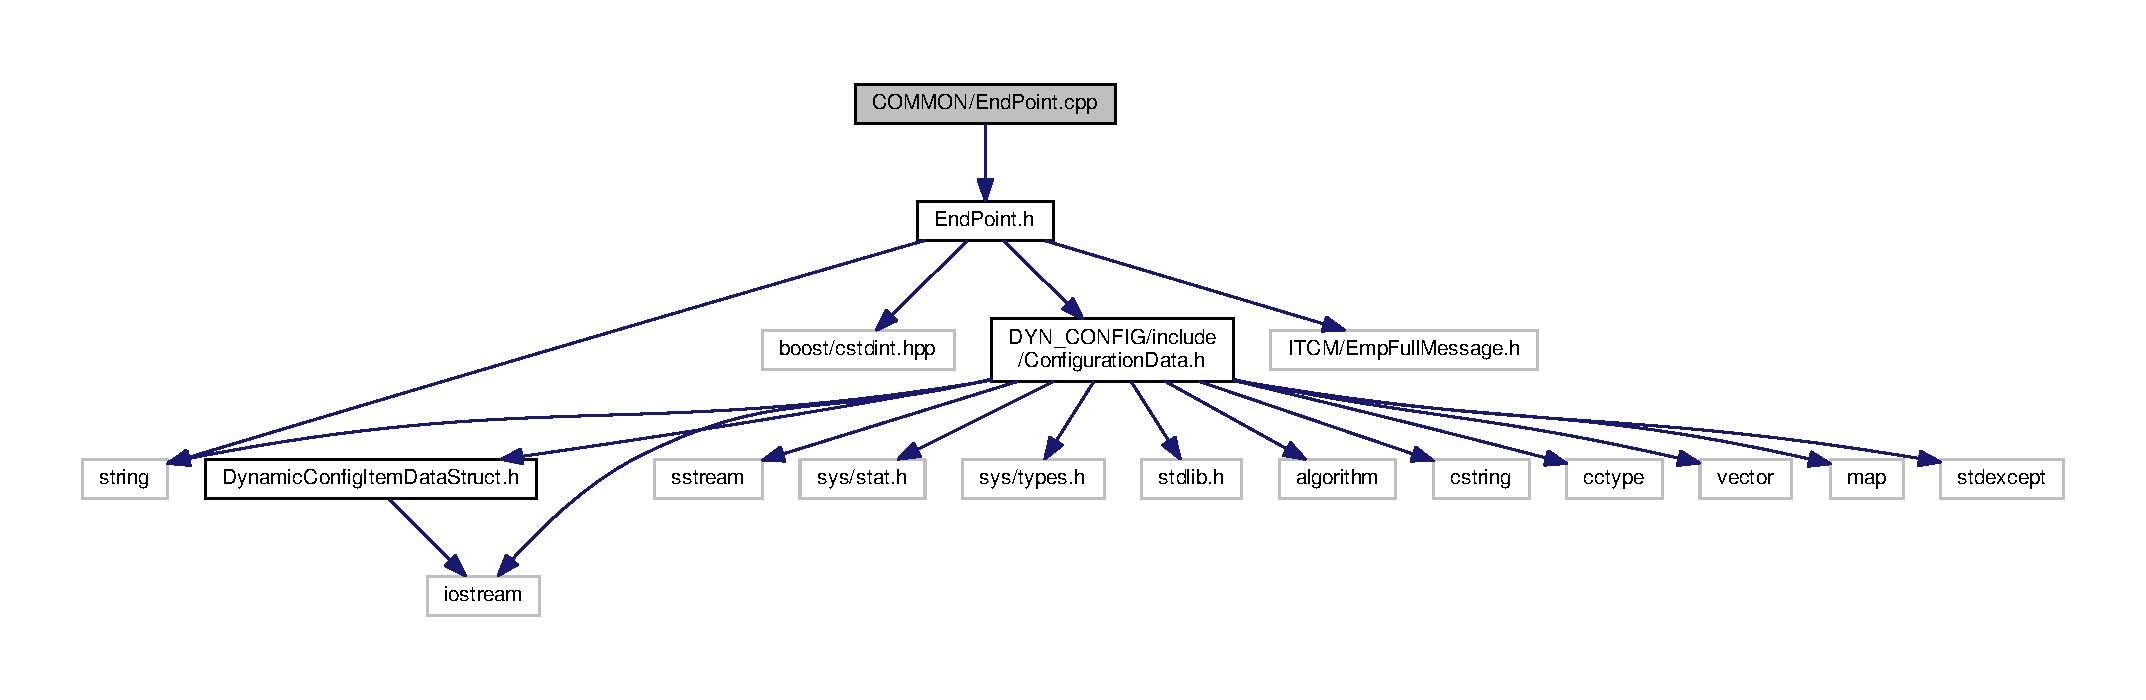
\includegraphics[width=350pt]{EndPoint_8cpp__incl}
\end{center}
\end{figure}

\hypertarget{EndPoint_8h}{}\section{C\+O\+M\+M\+O\+N/\+End\+Point.h File Reference}
\label{EndPoint_8h}\index{C\+O\+M\+M\+O\+N/\+End\+Point.\+h@{C\+O\+M\+M\+O\+N/\+End\+Point.\+h}}
{\ttfamily \#include $<$string$>$}\\*
{\ttfamily \#include $<$boost/cstdint.\+hpp$>$}\\*
{\ttfamily \#include \char`\"{}D\+Y\+N\+\_\+\+C\+O\+N\+F\+I\+G/include/\+Configuration\+Data.\+h\char`\"{}}\\*
{\ttfamily \#include \char`\"{}I\+T\+C\+M/\+Emp\+Full\+Message.\+h\char`\"{}}\\*
Include dependency graph for End\+Point.\+h\+:
\nopagebreak
\begin{figure}[H]
\begin{center}
\leavevmode
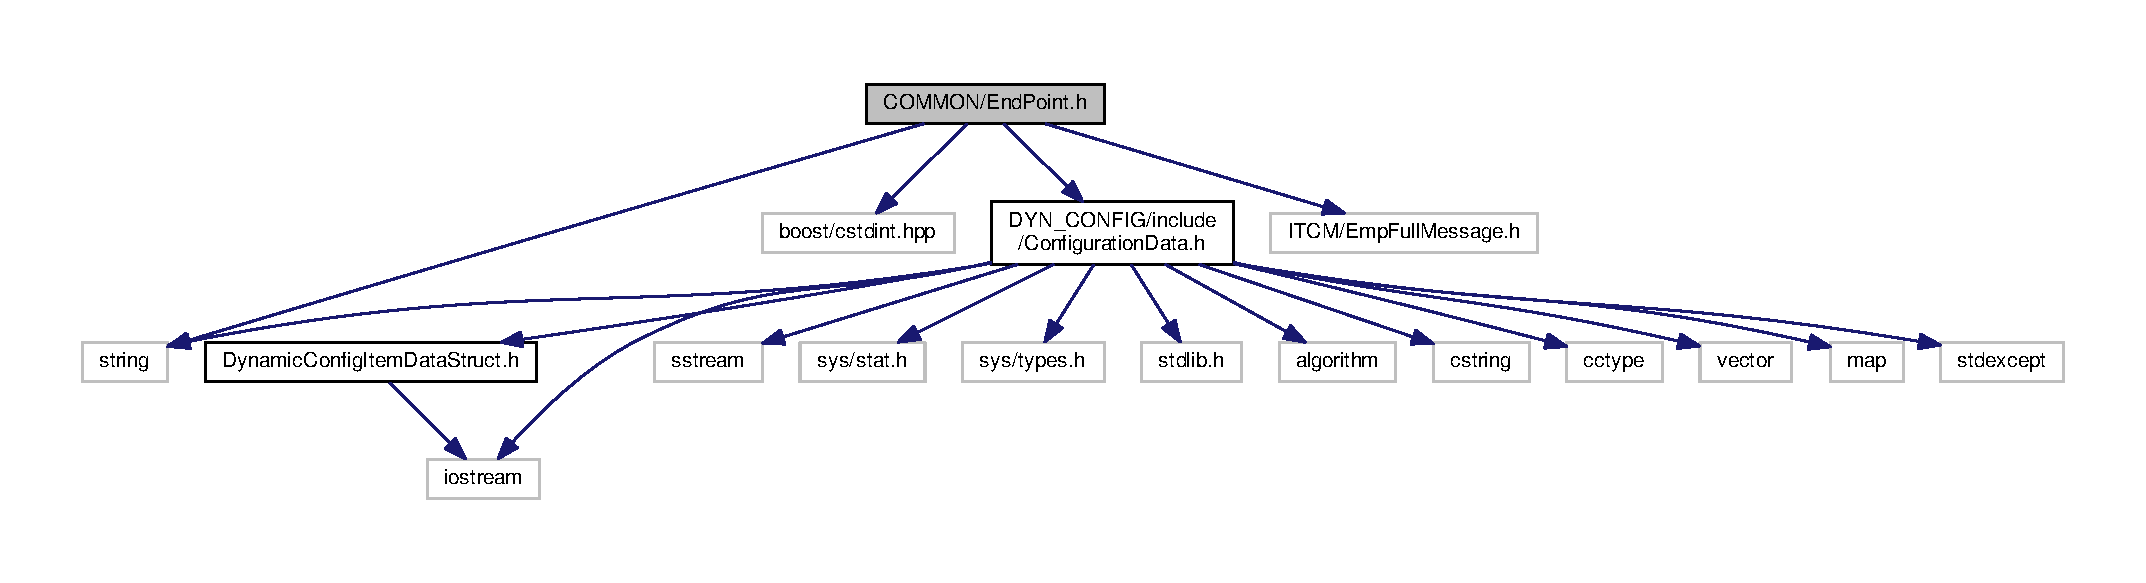
\includegraphics[width=350pt]{EndPoint_8h__incl}
\end{center}
\end{figure}
This graph shows which files directly or indirectly include this file\+:
\nopagebreak
\begin{figure}[H]
\begin{center}
\leavevmode
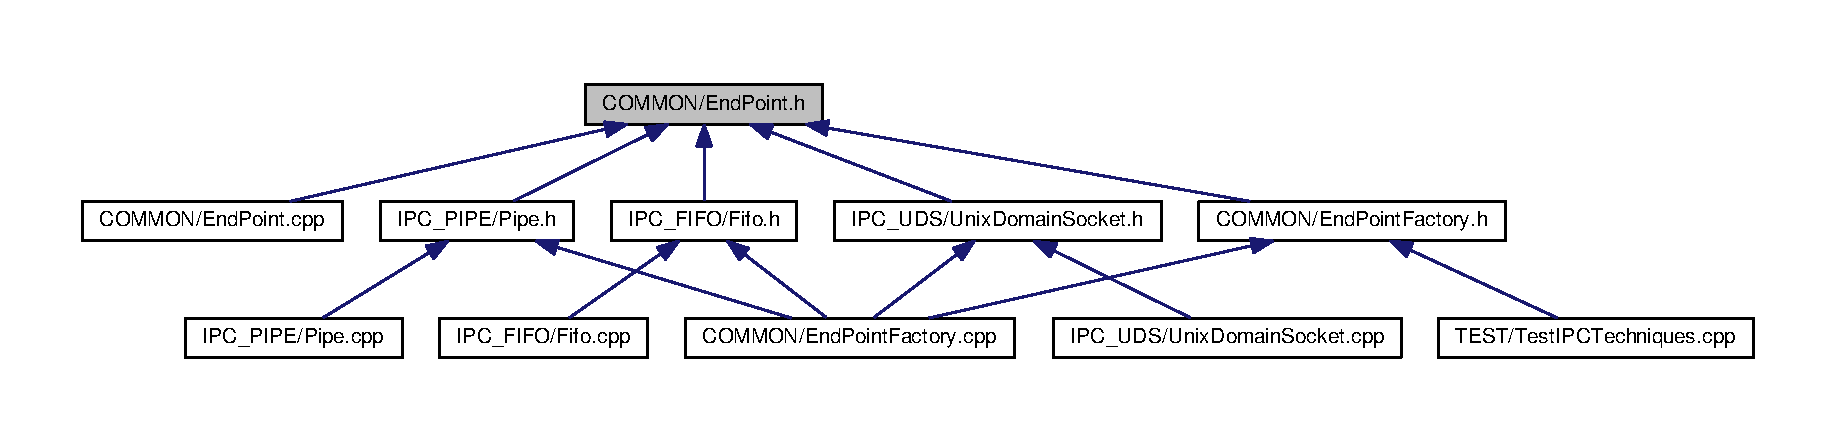
\includegraphics[width=350pt]{EndPoint_8h__dep__incl}
\end{center}
\end{figure}
\subsection*{Classes}
\begin{DoxyCompactItemize}
\item 
struct \hyperlink{structipc_1_1emp__message__part__before__length}{ipc\+::emp\+\_\+message\+\_\+part\+\_\+before\+\_\+length}
\item 
struct \hyperlink{structipc_1_1emp__message__part__after__length}{ipc\+::emp\+\_\+message\+\_\+part\+\_\+after\+\_\+length}
\item 
class \hyperlink{classipc_1_1EndPoint}{ipc\+::\+End\+Point}
\end{DoxyCompactItemize}
\subsection*{Namespaces}
\begin{DoxyCompactItemize}
\item 
 \hyperlink{namespaceipc}{ipc}
\end{DoxyCompactItemize}
\subsection*{Macros}
\begin{DoxyCompactItemize}
\item 
\#define \hyperlink{EndPoint_8h_a4cc22404ae783a0f4c410aaae085e2f1}{M\+A\+X\+\_\+\+E\+M\+P\+\_\+\+M\+E\+S\+S\+A\+G\+E\+\_\+\+L\+E\+N\+G\+TH}~1 $\ast$ 1024 $\ast$ 1024
\end{DoxyCompactItemize}


\subsection{Macro Definition Documentation}
\index{End\+Point.\+h@{End\+Point.\+h}!M\+A\+X\+\_\+\+E\+M\+P\+\_\+\+M\+E\+S\+S\+A\+G\+E\+\_\+\+L\+E\+N\+G\+TH@{M\+A\+X\+\_\+\+E\+M\+P\+\_\+\+M\+E\+S\+S\+A\+G\+E\+\_\+\+L\+E\+N\+G\+TH}}
\index{M\+A\+X\+\_\+\+E\+M\+P\+\_\+\+M\+E\+S\+S\+A\+G\+E\+\_\+\+L\+E\+N\+G\+TH@{M\+A\+X\+\_\+\+E\+M\+P\+\_\+\+M\+E\+S\+S\+A\+G\+E\+\_\+\+L\+E\+N\+G\+TH}!End\+Point.\+h@{End\+Point.\+h}}
\subsubsection[{\texorpdfstring{M\+A\+X\+\_\+\+E\+M\+P\+\_\+\+M\+E\+S\+S\+A\+G\+E\+\_\+\+L\+E\+N\+G\+TH}{MAX_EMP_MESSAGE_LENGTH}}]{\setlength{\rightskip}{0pt plus 5cm}\#define M\+A\+X\+\_\+\+E\+M\+P\+\_\+\+M\+E\+S\+S\+A\+G\+E\+\_\+\+L\+E\+N\+G\+TH~1 $\ast$ 1024 $\ast$ 1024}\hypertarget{EndPoint_8h_a4cc22404ae783a0f4c410aaae085e2f1}{}\label{EndPoint_8h_a4cc22404ae783a0f4c410aaae085e2f1}


Definition at line 29 of file End\+Point.\+h.


\hypertarget{EndPointFactory_8cpp}{}\section{C\+O\+M\+M\+O\+N/\+End\+Point\+Factory.cpp File Reference}
\label{EndPointFactory_8cpp}\index{C\+O\+M\+M\+O\+N/\+End\+Point\+Factory.\+cpp@{C\+O\+M\+M\+O\+N/\+End\+Point\+Factory.\+cpp}}
{\ttfamily \#include \char`\"{}End\+Point\+Factory.\+h\char`\"{}}\\*
{\ttfamily \#include \char`\"{}I\+P\+C\+\_\+\+P\+I\+P\+E/\+Pipe.\+h\char`\"{}}\\*
{\ttfamily \#include \char`\"{}I\+P\+C\+\_\+\+F\+I\+F\+O/\+Fifo.\+h\char`\"{}}\\*
{\ttfamily \#include \char`\"{}I\+P\+C\+\_\+\+U\+D\+S/\+Unix\+Domain\+Socket.\+h\char`\"{}}\\*
Include dependency graph for End\+Point\+Factory.\+cpp\+:
\nopagebreak
\begin{figure}[H]
\begin{center}
\leavevmode
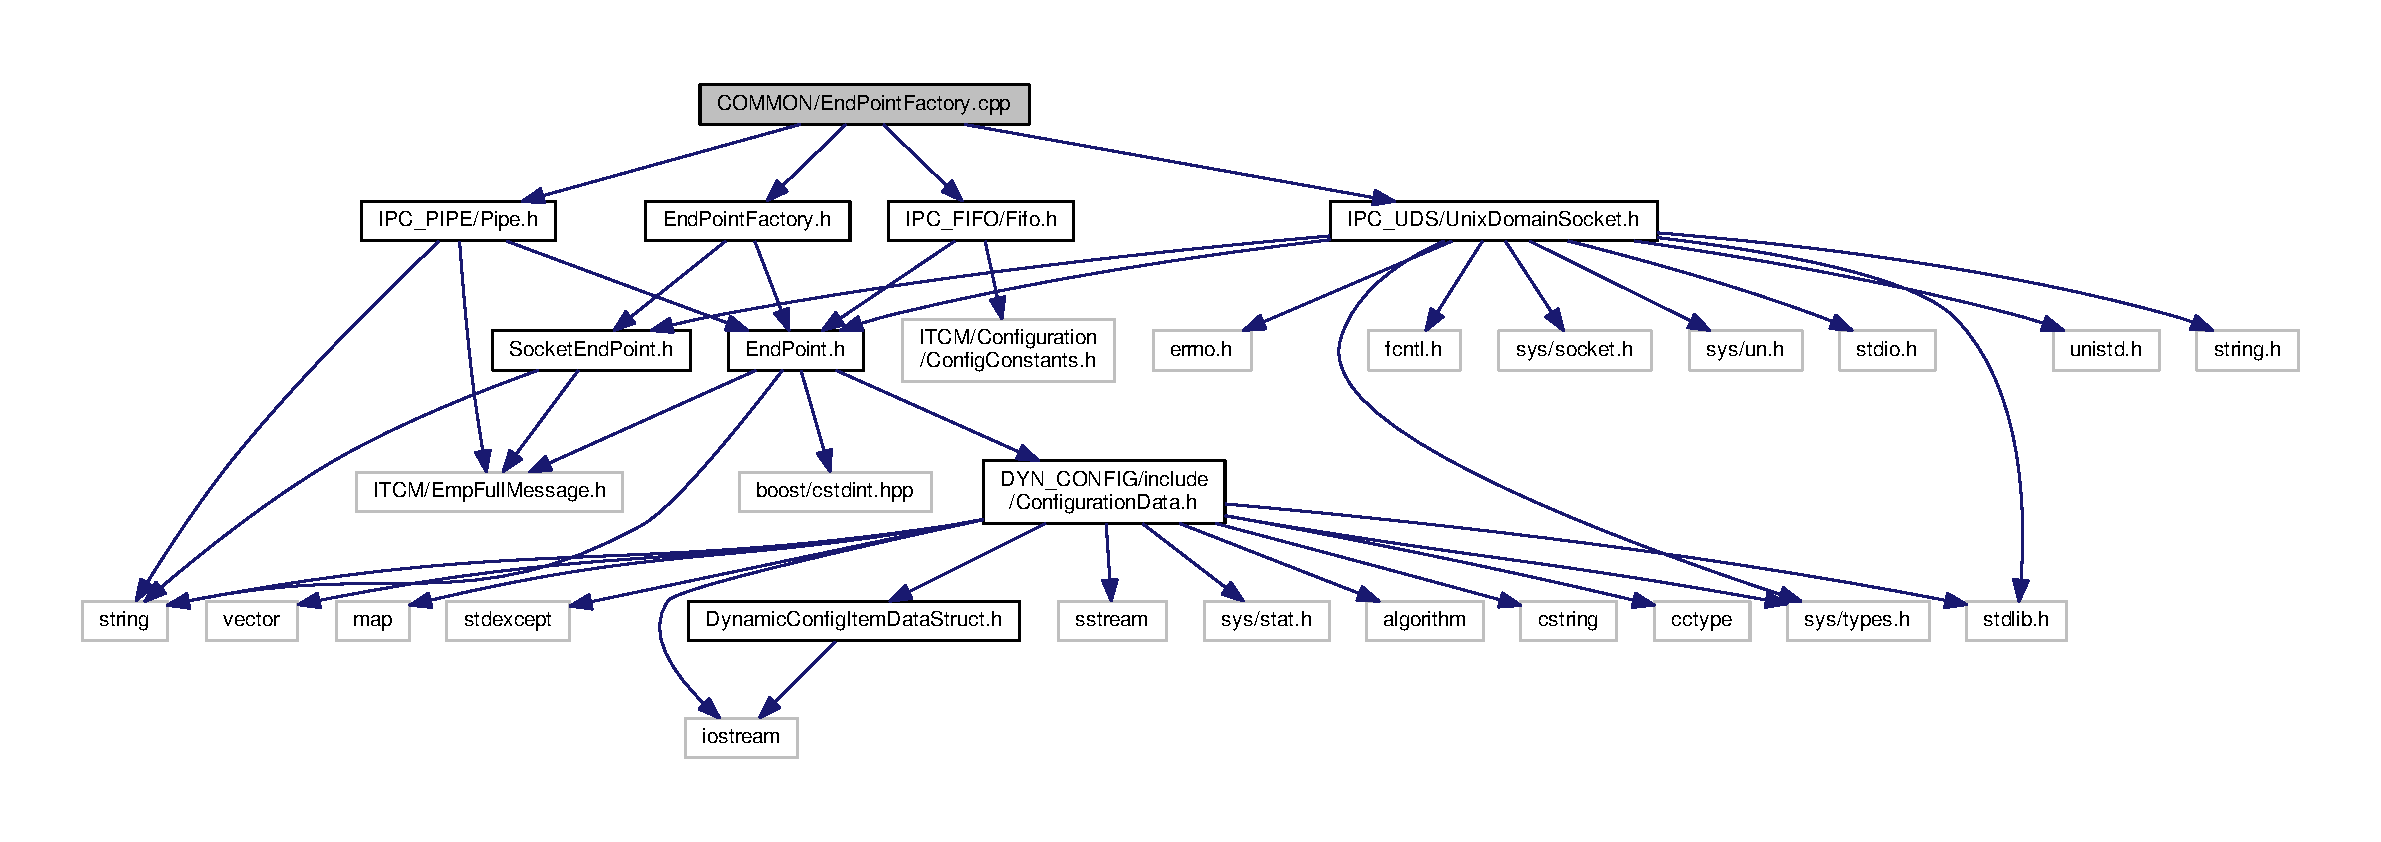
\includegraphics[width=350pt]{EndPointFactory_8cpp__incl}
\end{center}
\end{figure}

\hypertarget{EndPointFactory_8h}{}\section{C\+O\+M\+M\+O\+N/\+End\+Point\+Factory.h File Reference}
\label{EndPointFactory_8h}\index{C\+O\+M\+M\+O\+N/\+End\+Point\+Factory.\+h@{C\+O\+M\+M\+O\+N/\+End\+Point\+Factory.\+h}}
{\ttfamily \#include \char`\"{}End\+Point.\+h\char`\"{}}\\*
{\ttfamily \#include \char`\"{}Socket\+End\+Point.\+h\char`\"{}}\\*
Include dependency graph for End\+Point\+Factory.\+h\+:
\nopagebreak
\begin{figure}[H]
\begin{center}
\leavevmode
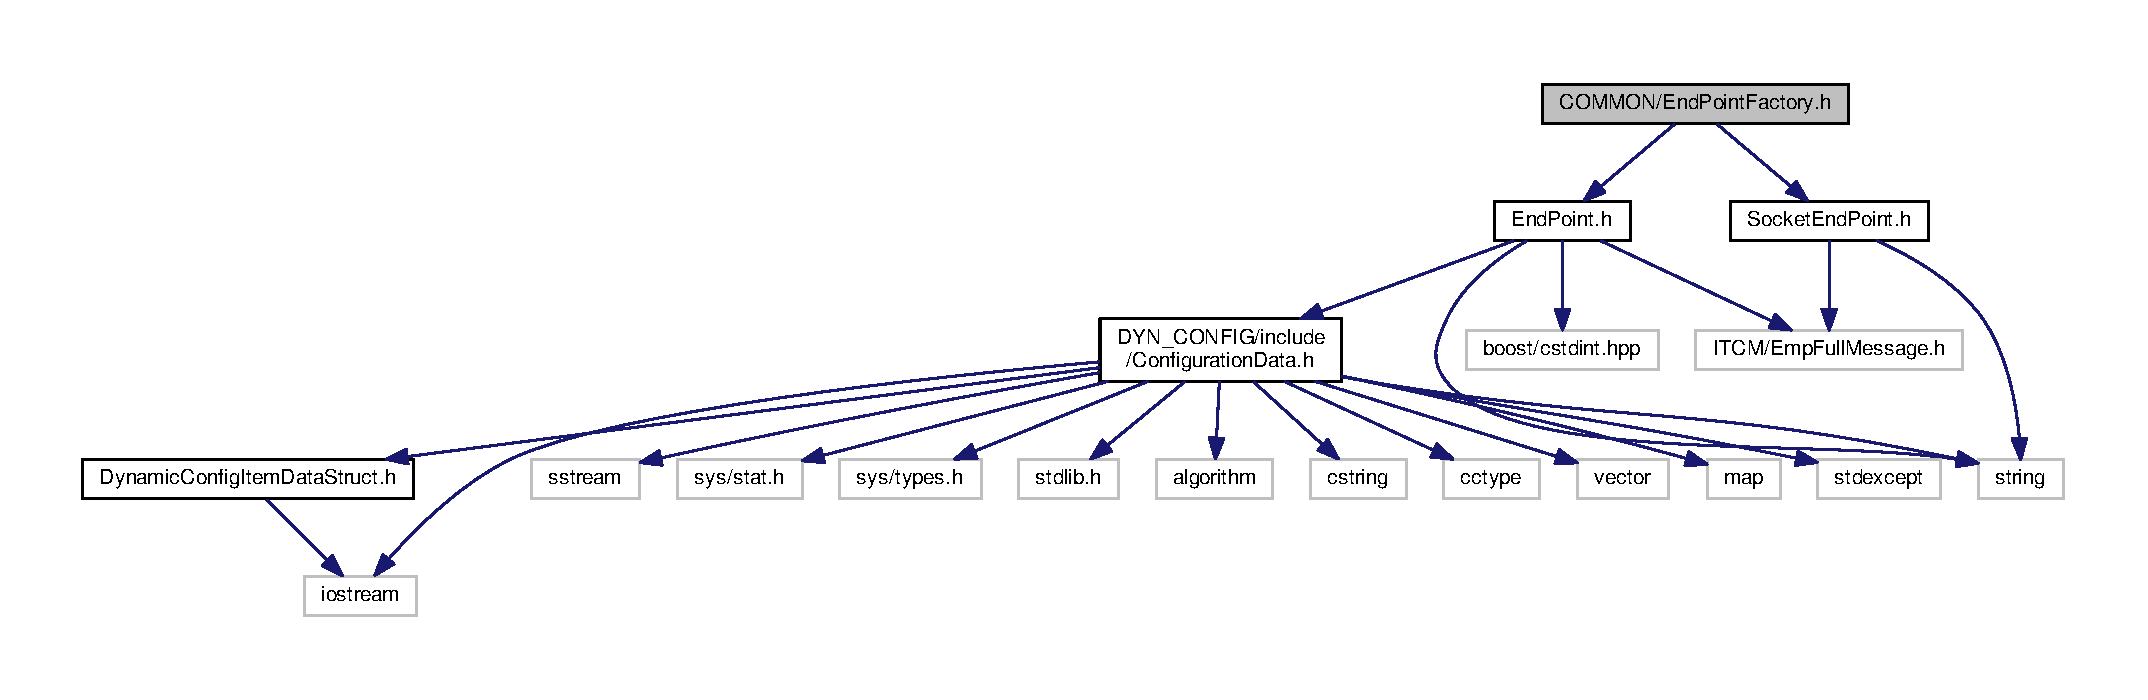
\includegraphics[width=350pt]{EndPointFactory_8h__incl}
\end{center}
\end{figure}
This graph shows which files directly or indirectly include this file\+:
\nopagebreak
\begin{figure}[H]
\begin{center}
\leavevmode
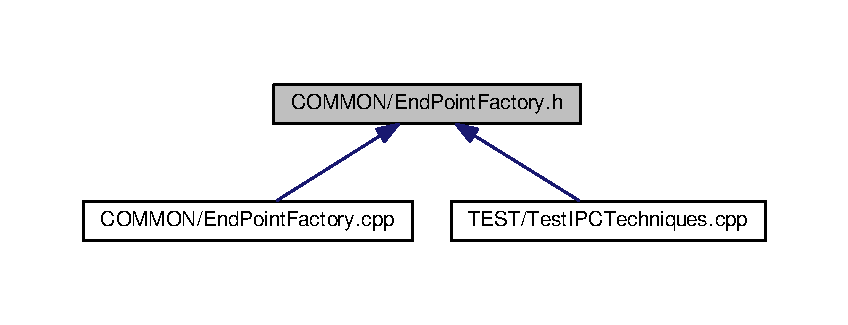
\includegraphics[width=350pt]{EndPointFactory_8h__dep__incl}
\end{center}
\end{figure}
\subsection*{Classes}
\begin{DoxyCompactItemize}
\item 
class \hyperlink{classipc_1_1EndPointFactory}{ipc\+::\+End\+Point\+Factory}
\end{DoxyCompactItemize}
\subsection*{Namespaces}
\begin{DoxyCompactItemize}
\item 
 \hyperlink{namespaceipc}{ipc}
\end{DoxyCompactItemize}
\subsection*{Macros}
\begin{DoxyCompactItemize}
\item 
\#define \hyperlink{EndPointFactory_8h_ad086ba1b5fcbd4373328901a98b20247}{E\+N\+D\+\_\+point\+\_\+\+F\+A\+C\+T\+O\+R\+Y\+\_\+\+H\+\_\+}
\end{DoxyCompactItemize}


\subsection{Macro Definition Documentation}
\index{End\+Point\+Factory.\+h@{End\+Point\+Factory.\+h}!E\+N\+D\+\_\+point\+\_\+\+F\+A\+C\+T\+O\+R\+Y\+\_\+\+H\+\_\+@{E\+N\+D\+\_\+point\+\_\+\+F\+A\+C\+T\+O\+R\+Y\+\_\+\+H\+\_\+}}
\index{E\+N\+D\+\_\+point\+\_\+\+F\+A\+C\+T\+O\+R\+Y\+\_\+\+H\+\_\+@{E\+N\+D\+\_\+point\+\_\+\+F\+A\+C\+T\+O\+R\+Y\+\_\+\+H\+\_\+}!End\+Point\+Factory.\+h@{End\+Point\+Factory.\+h}}
\subsubsection[{\texorpdfstring{E\+N\+D\+\_\+point\+\_\+\+F\+A\+C\+T\+O\+R\+Y\+\_\+\+H\+\_\+}{END_point_FACTORY_H_}}]{\setlength{\rightskip}{0pt plus 5cm}\#define E\+N\+D\+\_\+point\+\_\+\+F\+A\+C\+T\+O\+R\+Y\+\_\+\+H\+\_\+}\hypertarget{EndPointFactory_8h_ad086ba1b5fcbd4373328901a98b20247}{}\label{EndPointFactory_8h_ad086ba1b5fcbd4373328901a98b20247}


Definition at line 3 of file End\+Point\+Factory.\+h.


\hypertarget{SocketEndPoint_8cpp}{}\section{C\+O\+M\+M\+O\+N/\+Socket\+End\+Point.cpp File Reference}
\label{SocketEndPoint_8cpp}\index{C\+O\+M\+M\+O\+N/\+Socket\+End\+Point.\+cpp@{C\+O\+M\+M\+O\+N/\+Socket\+End\+Point.\+cpp}}
{\ttfamily \#include \char`\"{}Socket\+End\+Point.\+h\char`\"{}}\\*
Include dependency graph for Socket\+End\+Point.\+cpp\+:
\nopagebreak
\begin{figure}[H]
\begin{center}
\leavevmode
\includegraphics[width=273pt]{SocketEndPoint_8cpp__incl}
\end{center}
\end{figure}

\hypertarget{SocketEndPoint_8h}{}\section{C\+O\+M\+M\+O\+N/\+Socket\+End\+Point.h File Reference}
\label{SocketEndPoint_8h}\index{C\+O\+M\+M\+O\+N/\+Socket\+End\+Point.\+h@{C\+O\+M\+M\+O\+N/\+Socket\+End\+Point.\+h}}
{\ttfamily \#include $<$string$>$}\\*
{\ttfamily \#include \char`\"{}I\+T\+C\+M/\+Emp\+Full\+Message.\+h\char`\"{}}\\*
Include dependency graph for Socket\+End\+Point.\+h\+:
\nopagebreak
\begin{figure}[H]
\begin{center}
\leavevmode
\includegraphics[width=268pt]{SocketEndPoint_8h__incl}
\end{center}
\end{figure}
This graph shows which files directly or indirectly include this file\+:
\nopagebreak
\begin{figure}[H]
\begin{center}
\leavevmode
\includegraphics[width=350pt]{SocketEndPoint_8h__dep__incl}
\end{center}
\end{figure}
\subsection*{Classes}
\begin{DoxyCompactItemize}
\item 
class \hyperlink{classipc_1_1SocketEndPoint}{ipc\+::\+Socket\+End\+Point}
\end{DoxyCompactItemize}
\subsection*{Namespaces}
\begin{DoxyCompactItemize}
\item 
 \hyperlink{namespaceipc}{ipc}
\end{DoxyCompactItemize}

\hypertarget{EndPoint_8d}{}\section{Debug/\+C\+O\+M\+M\+O\+N/\+End\+Point.d File Reference}
\label{EndPoint_8d}\index{Debug/\+C\+O\+M\+M\+O\+N/\+End\+Point.\+d@{Debug/\+C\+O\+M\+M\+O\+N/\+End\+Point.\+d}}

\hypertarget{EndPointFactory_8d}{}\section{Debug/\+C\+O\+M\+M\+O\+N/\+End\+Point\+Factory.d File Reference}
\label{EndPointFactory_8d}\index{Debug/\+C\+O\+M\+M\+O\+N/\+End\+Point\+Factory.\+d@{Debug/\+C\+O\+M\+M\+O\+N/\+End\+Point\+Factory.\+d}}

\hypertarget{MessageReader_8d}{}\section{Debug/\+C\+O\+M\+M\+O\+N/\+Message\+Reader.d File Reference}
\label{MessageReader_8d}\index{Debug/\+C\+O\+M\+M\+O\+N/\+Message\+Reader.\+d@{Debug/\+C\+O\+M\+M\+O\+N/\+Message\+Reader.\+d}}

\hypertarget{SocketEndPoint_8d}{}\section{Debug/\+C\+O\+M\+M\+O\+N/\+Socket\+End\+Point.d File Reference}
\label{SocketEndPoint_8d}\index{Debug/\+C\+O\+M\+M\+O\+N/\+Socket\+End\+Point.\+d@{Debug/\+C\+O\+M\+M\+O\+N/\+Socket\+End\+Point.\+d}}

\hypertarget{Fifo_8d}{}\section{Debug/\+I\+P\+C\+\_\+\+F\+I\+F\+O/\+Fifo.d File Reference}
\label{Fifo_8d}\index{Debug/\+I\+P\+C\+\_\+\+F\+I\+F\+O/\+Fifo.\+d@{Debug/\+I\+P\+C\+\_\+\+F\+I\+F\+O/\+Fifo.\+d}}

\hypertarget{Pipe_8d}{}\section{Debug/\+I\+P\+C\+\_\+\+P\+I\+P\+E/\+Pipe.d File Reference}
\label{Pipe_8d}\index{Debug/\+I\+P\+C\+\_\+\+P\+I\+P\+E/\+Pipe.\+d@{Debug/\+I\+P\+C\+\_\+\+P\+I\+P\+E/\+Pipe.\+d}}

\hypertarget{UnixDomainSocket_8d}{}\section{Debug/\+I\+P\+C\+\_\+\+U\+D\+S/\+Unix\+Domain\+Socket.d File Reference}
\label{UnixDomainSocket_8d}\index{Debug/\+I\+P\+C\+\_\+\+U\+D\+S/\+Unix\+Domain\+Socket.\+d@{Debug/\+I\+P\+C\+\_\+\+U\+D\+S/\+Unix\+Domain\+Socket.\+d}}

\hypertarget{Log_8d}{}\section{Debug/\+L\+O\+G/\+Log.d File Reference}
\label{Log_8d}\index{Debug/\+L\+O\+G/\+Log.\+d@{Debug/\+L\+O\+G/\+Log.\+d}}

\hypertarget{main_8d}{}\section{Debug/\+L\+O\+G/main.d File Reference}
\label{main_8d}\index{Debug/\+L\+O\+G/main.\+d@{Debug/\+L\+O\+G/main.\+d}}

\hypertarget{GtestMain_8d}{}\section{Debug/\+T\+E\+S\+T/\+Gtest\+Main.d File Reference}
\label{GtestMain_8d}\index{Debug/\+T\+E\+S\+T/\+Gtest\+Main.\+d@{Debug/\+T\+E\+S\+T/\+Gtest\+Main.\+d}}

\hypertarget{TestIPCTechniques_8d}{}\section{Debug/\+T\+E\+S\+T/\+Test\+I\+P\+C\+Techniques.d File Reference}
\label{TestIPCTechniques_8d}\index{Debug/\+T\+E\+S\+T/\+Test\+I\+P\+C\+Techniques.\+d@{Debug/\+T\+E\+S\+T/\+Test\+I\+P\+C\+Techniques.\+d}}

\hypertarget{ConfigurationData_8h}{}\section{D\+Y\+N\+\_\+\+C\+O\+N\+F\+I\+G/include/\+Configuration\+Data.h File Reference}
\label{ConfigurationData_8h}\index{D\+Y\+N\+\_\+\+C\+O\+N\+F\+I\+G/include/\+Configuration\+Data.\+h@{D\+Y\+N\+\_\+\+C\+O\+N\+F\+I\+G/include/\+Configuration\+Data.\+h}}
{\ttfamily \#include \char`\"{}Dynamic\+Config\+Item\+Data\+Struct.\+h\char`\"{}}\\*
{\ttfamily \#include $<$iostream$>$}\\*
{\ttfamily \#include $<$string$>$}\\*
{\ttfamily \#include $<$sstream$>$}\\*
{\ttfamily \#include $<$sys/stat.\+h$>$}\\*
{\ttfamily \#include $<$sys/types.\+h$>$}\\*
{\ttfamily \#include $<$stdlib.\+h$>$}\\*
{\ttfamily \#include $<$algorithm$>$}\\*
{\ttfamily \#include $<$cstring$>$}\\*
{\ttfamily \#include $<$cctype$>$}\\*
{\ttfamily \#include $<$vector$>$}\\*
{\ttfamily \#include $<$map$>$}\\*
{\ttfamily \#include $<$stdexcept$>$}\\*
Include dependency graph for Configuration\+Data.\+h\+:
\nopagebreak
\begin{figure}[H]
\begin{center}
\leavevmode
\includegraphics[width=350pt]{ConfigurationData_8h__incl}
\end{center}
\end{figure}
This graph shows which files directly or indirectly include this file\+:
\nopagebreak
\begin{figure}[H]
\begin{center}
\leavevmode
\includegraphics[width=350pt]{ConfigurationData_8h__dep__incl}
\end{center}
\end{figure}
\subsection*{Classes}
\begin{DoxyCompactItemize}
\item 
class \hyperlink{classConfigurationData}{Configuration\+Data}
\end{DoxyCompactItemize}
\subsection*{Enumerations}
\begin{DoxyCompactItemize}
\item 
enum \hyperlink{ConfigurationData_8h_a4e9a8de26cf7d053d8e1db76220bdc33}{Dyn\+Cfg\+Intf\+Return\+Codes} \{ \hyperlink{ConfigurationData_8h_a4e9a8de26cf7d053d8e1db76220bdc33a9700005fb727365536f5e59c3ff8ae3f}{D\+Y\+N\+C\+F\+G\+\_\+\+L\+O\+A\+D\+\_\+\+N\+O\+T\+\_\+\+N\+E\+E\+D\+ED}, 
\hyperlink{ConfigurationData_8h_a4e9a8de26cf7d053d8e1db76220bdc33aaac28f98110a624c5fd27f389e4324dd}{D\+Y\+N\+C\+F\+G\+\_\+\+L\+O\+A\+D\+\_\+\+O\+K\+AY}, 
\hyperlink{ConfigurationData_8h_a4e9a8de26cf7d053d8e1db76220bdc33a9dd06682c59708308d169e3a2a53fd06}{D\+Y\+N\+C\+F\+G\+\_\+\+L\+O\+A\+D\+\_\+\+F\+A\+I\+L\+ED}
 \}
\end{DoxyCompactItemize}
\subsection*{Variables}
\begin{DoxyCompactItemize}
\item 
const std\+::string \hyperlink{ConfigurationData_8h_a1bb8c863dd324166ab7ef7ef053bcd5d}{D\+E\+F\+A\+U\+L\+T\+\_\+\+D\+Y\+N\+C\+FG} = \char`\"{}Configuration\char`\"{}
\end{DoxyCompactItemize}


\subsection{Enumeration Type Documentation}
\index{Configuration\+Data.\+h@{Configuration\+Data.\+h}!Dyn\+Cfg\+Intf\+Return\+Codes@{Dyn\+Cfg\+Intf\+Return\+Codes}}
\index{Dyn\+Cfg\+Intf\+Return\+Codes@{Dyn\+Cfg\+Intf\+Return\+Codes}!Configuration\+Data.\+h@{Configuration\+Data.\+h}}
\subsubsection[{\texorpdfstring{Dyn\+Cfg\+Intf\+Return\+Codes}{DynCfgIntfReturnCodes}}]{\setlength{\rightskip}{0pt plus 5cm}enum {\bf Dyn\+Cfg\+Intf\+Return\+Codes}}\hypertarget{ConfigurationData_8h_a4e9a8de26cf7d053d8e1db76220bdc33}{}\label{ConfigurationData_8h_a4e9a8de26cf7d053d8e1db76220bdc33}
\begin{Desc}
\item[Enumerator]\par
\begin{description}
\index{D\+Y\+N\+C\+F\+G\+\_\+\+L\+O\+A\+D\+\_\+\+N\+O\+T\+\_\+\+N\+E\+E\+D\+ED@{D\+Y\+N\+C\+F\+G\+\_\+\+L\+O\+A\+D\+\_\+\+N\+O\+T\+\_\+\+N\+E\+E\+D\+ED}!Configuration\+Data.\+h@{Configuration\+Data.\+h}}\index{Configuration\+Data.\+h@{Configuration\+Data.\+h}!D\+Y\+N\+C\+F\+G\+\_\+\+L\+O\+A\+D\+\_\+\+N\+O\+T\+\_\+\+N\+E\+E\+D\+ED@{D\+Y\+N\+C\+F\+G\+\_\+\+L\+O\+A\+D\+\_\+\+N\+O\+T\+\_\+\+N\+E\+E\+D\+ED}}\item[{\em 
D\+Y\+N\+C\+F\+G\+\_\+\+L\+O\+A\+D\+\_\+\+N\+O\+T\+\_\+\+N\+E\+E\+D\+ED\hypertarget{ConfigurationData_8h_a4e9a8de26cf7d053d8e1db76220bdc33a9700005fb727365536f5e59c3ff8ae3f}{}\label{ConfigurationData_8h_a4e9a8de26cf7d053d8e1db76220bdc33a9700005fb727365536f5e59c3ff8ae3f}
}]\index{D\+Y\+N\+C\+F\+G\+\_\+\+L\+O\+A\+D\+\_\+\+O\+K\+AY@{D\+Y\+N\+C\+F\+G\+\_\+\+L\+O\+A\+D\+\_\+\+O\+K\+AY}!Configuration\+Data.\+h@{Configuration\+Data.\+h}}\index{Configuration\+Data.\+h@{Configuration\+Data.\+h}!D\+Y\+N\+C\+F\+G\+\_\+\+L\+O\+A\+D\+\_\+\+O\+K\+AY@{D\+Y\+N\+C\+F\+G\+\_\+\+L\+O\+A\+D\+\_\+\+O\+K\+AY}}\item[{\em 
D\+Y\+N\+C\+F\+G\+\_\+\+L\+O\+A\+D\+\_\+\+O\+K\+AY\hypertarget{ConfigurationData_8h_a4e9a8de26cf7d053d8e1db76220bdc33aaac28f98110a624c5fd27f389e4324dd}{}\label{ConfigurationData_8h_a4e9a8de26cf7d053d8e1db76220bdc33aaac28f98110a624c5fd27f389e4324dd}
}]\index{D\+Y\+N\+C\+F\+G\+\_\+\+L\+O\+A\+D\+\_\+\+F\+A\+I\+L\+ED@{D\+Y\+N\+C\+F\+G\+\_\+\+L\+O\+A\+D\+\_\+\+F\+A\+I\+L\+ED}!Configuration\+Data.\+h@{Configuration\+Data.\+h}}\index{Configuration\+Data.\+h@{Configuration\+Data.\+h}!D\+Y\+N\+C\+F\+G\+\_\+\+L\+O\+A\+D\+\_\+\+F\+A\+I\+L\+ED@{D\+Y\+N\+C\+F\+G\+\_\+\+L\+O\+A\+D\+\_\+\+F\+A\+I\+L\+ED}}\item[{\em 
D\+Y\+N\+C\+F\+G\+\_\+\+L\+O\+A\+D\+\_\+\+F\+A\+I\+L\+ED\hypertarget{ConfigurationData_8h_a4e9a8de26cf7d053d8e1db76220bdc33a9dd06682c59708308d169e3a2a53fd06}{}\label{ConfigurationData_8h_a4e9a8de26cf7d053d8e1db76220bdc33a9dd06682c59708308d169e3a2a53fd06}
}]\end{description}
\end{Desc}


Definition at line 23 of file Configuration\+Data.\+h.



\subsection{Variable Documentation}
\index{Configuration\+Data.\+h@{Configuration\+Data.\+h}!D\+E\+F\+A\+U\+L\+T\+\_\+\+D\+Y\+N\+C\+FG@{D\+E\+F\+A\+U\+L\+T\+\_\+\+D\+Y\+N\+C\+FG}}
\index{D\+E\+F\+A\+U\+L\+T\+\_\+\+D\+Y\+N\+C\+FG@{D\+E\+F\+A\+U\+L\+T\+\_\+\+D\+Y\+N\+C\+FG}!Configuration\+Data.\+h@{Configuration\+Data.\+h}}
\subsubsection[{\texorpdfstring{D\+E\+F\+A\+U\+L\+T\+\_\+\+D\+Y\+N\+C\+FG}{DEFAULT_DYNCFG}}]{\setlength{\rightskip}{0pt plus 5cm}const std\+::string D\+E\+F\+A\+U\+L\+T\+\_\+\+D\+Y\+N\+C\+FG = \char`\"{}Configuration\char`\"{}}\hypertarget{ConfigurationData_8h_a1bb8c863dd324166ab7ef7ef053bcd5d}{}\label{ConfigurationData_8h_a1bb8c863dd324166ab7ef7ef053bcd5d}


Definition at line 21 of file Configuration\+Data.\+h.


\hypertarget{ConfigurationDataFromDatabase_8h}{}\section{D\+Y\+N\+\_\+\+C\+O\+N\+F\+I\+G/include/\+Configuration\+Data\+From\+Database.h File Reference}
\label{ConfigurationDataFromDatabase_8h}\index{D\+Y\+N\+\_\+\+C\+O\+N\+F\+I\+G/include/\+Configuration\+Data\+From\+Database.\+h@{D\+Y\+N\+\_\+\+C\+O\+N\+F\+I\+G/include/\+Configuration\+Data\+From\+Database.\+h}}
{\ttfamily \#include $<$iostream$>$}\\*
{\ttfamily \#include $<$string.\+h$>$}\\*
{\ttfamily \#include $<$sys/stat.\+h$>$}\\*
{\ttfamily \#include $<$sys/types.\+h$>$}\\*
{\ttfamily \#include $<$stdlib.\+h$>$}\\*
{\ttfamily \#include $<$algorithm$>$}\\*
{\ttfamily \#include $<$cstring$>$}\\*
{\ttfamily \#include $<$cctype$>$}\\*
{\ttfamily \#include $<$vector$>$}\\*
{\ttfamily \#include $<$map$>$}\\*
{\ttfamily \#include \char`\"{}Dynamic\+Config\+Item\+Data\+Struct.\+h\char`\"{}}\\*
Include dependency graph for Configuration\+Data\+From\+Database.\+h\+:
\nopagebreak
\begin{figure}[H]
\begin{center}
\leavevmode
\includegraphics[width=350pt]{ConfigurationDataFromDatabase_8h__incl}
\end{center}
\end{figure}
\subsection*{Classes}
\begin{DoxyCompactItemize}
\item 
class \hyperlink{classConfigurationDataFromDatabase}{Configuration\+Data\+From\+Database}
\end{DoxyCompactItemize}
\subsection*{Variables}
\begin{DoxyCompactItemize}
\item 
const int \hyperlink{ConfigurationDataFromDatabase_8h_a6e392370bd440c3edd8c168172e1ea08}{max\+\_\+msg\+\_\+size\+\_\+c} = 1024
\end{DoxyCompactItemize}


\subsection{Variable Documentation}
\index{Configuration\+Data\+From\+Database.\+h@{Configuration\+Data\+From\+Database.\+h}!max\+\_\+msg\+\_\+size\+\_\+c@{max\+\_\+msg\+\_\+size\+\_\+c}}
\index{max\+\_\+msg\+\_\+size\+\_\+c@{max\+\_\+msg\+\_\+size\+\_\+c}!Configuration\+Data\+From\+Database.\+h@{Configuration\+Data\+From\+Database.\+h}}
\subsubsection[{\texorpdfstring{max\+\_\+msg\+\_\+size\+\_\+c}{max_msg_size_c}}]{\setlength{\rightskip}{0pt plus 5cm}const int max\+\_\+msg\+\_\+size\+\_\+c = 1024}\hypertarget{ConfigurationDataFromDatabase_8h_a6e392370bd440c3edd8c168172e1ea08}{}\label{ConfigurationDataFromDatabase_8h_a6e392370bd440c3edd8c168172e1ea08}


Definition at line 19 of file Configuration\+Data\+From\+Database.\+h.


\hypertarget{DatabaseDetails_8h}{}\section{D\+Y\+N\+\_\+\+C\+O\+N\+F\+I\+G/include/\+Database\+Details.h File Reference}
\label{DatabaseDetails_8h}\index{D\+Y\+N\+\_\+\+C\+O\+N\+F\+I\+G/include/\+Database\+Details.\+h@{D\+Y\+N\+\_\+\+C\+O\+N\+F\+I\+G/include/\+Database\+Details.\+h}}
{\ttfamily \#include $<$string$>$}\\*
Include dependency graph for Database\+Details.\+h\+:
\nopagebreak
\begin{figure}[H]
\begin{center}
\leavevmode
\includegraphics[width=196pt]{DatabaseDetails_8h__incl}
\end{center}
\end{figure}
This graph shows which files directly or indirectly include this file\+:
\nopagebreak
\begin{figure}[H]
\begin{center}
\leavevmode
\includegraphics[width=196pt]{DatabaseDetails_8h__dep__incl}
\end{center}
\end{figure}
\subsection*{Classes}
\begin{DoxyCompactItemize}
\item 
class \hyperlink{classDatabaseDetails}{Database\+Details}
\end{DoxyCompactItemize}

\hypertarget{DynamicConfigItemDataStruct_8h}{}\section{D\+Y\+N\+\_\+\+C\+O\+N\+F\+I\+G/include/\+Dynamic\+Config\+Item\+Data\+Struct.h File Reference}
\label{DynamicConfigItemDataStruct_8h}\index{D\+Y\+N\+\_\+\+C\+O\+N\+F\+I\+G/include/\+Dynamic\+Config\+Item\+Data\+Struct.\+h@{D\+Y\+N\+\_\+\+C\+O\+N\+F\+I\+G/include/\+Dynamic\+Config\+Item\+Data\+Struct.\+h}}
{\ttfamily \#include $<$iostream$>$}\\*
Include dependency graph for Dynamic\+Config\+Item\+Data\+Struct.\+h\+:
\nopagebreak
\begin{figure}[H]
\begin{center}
\leavevmode
\includegraphics[width=242pt]{DynamicConfigItemDataStruct_8h__incl}
\end{center}
\end{figure}
This graph shows which files directly or indirectly include this file\+:
\nopagebreak
\begin{figure}[H]
\begin{center}
\leavevmode
\includegraphics[width=350pt]{DynamicConfigItemDataStruct_8h__dep__incl}
\end{center}
\end{figure}
\subsection*{Classes}
\begin{DoxyCompactItemize}
\item 
struct \hyperlink{structDynamicConfigItemDataStruct}{Dynamic\+Config\+Item\+Data\+Struct}
\end{DoxyCompactItemize}
\subsection*{Variables}
\begin{DoxyCompactItemize}
\item 
const int \hyperlink{DynamicConfigItemDataStruct_8h_a856963f31e35df3fa9c1dc12c397f6be}{max\+\_\+item\+\_\+value\+\_\+size\+\_\+c} = 256
\item 
const int \hyperlink{DynamicConfigItemDataStruct_8h_a36ad3a2b20f9ec19b16064c421b6e953}{max\+\_\+item\+\_\+name\+\_\+size\+\_\+c} = 41
\item 
const int \hyperlink{DynamicConfigItemDataStruct_8h_abe9e708509ade3a5605d85dd5c0593ce}{max\+\_\+item\+\_\+value\+\_\+type\+\_\+size\+\_\+c} = 13
\end{DoxyCompactItemize}


\subsection{Variable Documentation}
\index{Dynamic\+Config\+Item\+Data\+Struct.\+h@{Dynamic\+Config\+Item\+Data\+Struct.\+h}!max\+\_\+item\+\_\+name\+\_\+size\+\_\+c@{max\+\_\+item\+\_\+name\+\_\+size\+\_\+c}}
\index{max\+\_\+item\+\_\+name\+\_\+size\+\_\+c@{max\+\_\+item\+\_\+name\+\_\+size\+\_\+c}!Dynamic\+Config\+Item\+Data\+Struct.\+h@{Dynamic\+Config\+Item\+Data\+Struct.\+h}}
\subsubsection[{\texorpdfstring{max\+\_\+item\+\_\+name\+\_\+size\+\_\+c}{max_item_name_size_c}}]{\setlength{\rightskip}{0pt plus 5cm}const int max\+\_\+item\+\_\+name\+\_\+size\+\_\+c = 41}\hypertarget{DynamicConfigItemDataStruct_8h_a36ad3a2b20f9ec19b16064c421b6e953}{}\label{DynamicConfigItemDataStruct_8h_a36ad3a2b20f9ec19b16064c421b6e953}


Definition at line 7 of file Dynamic\+Config\+Item\+Data\+Struct.\+h.

\index{Dynamic\+Config\+Item\+Data\+Struct.\+h@{Dynamic\+Config\+Item\+Data\+Struct.\+h}!max\+\_\+item\+\_\+value\+\_\+size\+\_\+c@{max\+\_\+item\+\_\+value\+\_\+size\+\_\+c}}
\index{max\+\_\+item\+\_\+value\+\_\+size\+\_\+c@{max\+\_\+item\+\_\+value\+\_\+size\+\_\+c}!Dynamic\+Config\+Item\+Data\+Struct.\+h@{Dynamic\+Config\+Item\+Data\+Struct.\+h}}
\subsubsection[{\texorpdfstring{max\+\_\+item\+\_\+value\+\_\+size\+\_\+c}{max_item_value_size_c}}]{\setlength{\rightskip}{0pt plus 5cm}const int max\+\_\+item\+\_\+value\+\_\+size\+\_\+c = 256}\hypertarget{DynamicConfigItemDataStruct_8h_a856963f31e35df3fa9c1dc12c397f6be}{}\label{DynamicConfigItemDataStruct_8h_a856963f31e35df3fa9c1dc12c397f6be}


Definition at line 6 of file Dynamic\+Config\+Item\+Data\+Struct.\+h.

\index{Dynamic\+Config\+Item\+Data\+Struct.\+h@{Dynamic\+Config\+Item\+Data\+Struct.\+h}!max\+\_\+item\+\_\+value\+\_\+type\+\_\+size\+\_\+c@{max\+\_\+item\+\_\+value\+\_\+type\+\_\+size\+\_\+c}}
\index{max\+\_\+item\+\_\+value\+\_\+type\+\_\+size\+\_\+c@{max\+\_\+item\+\_\+value\+\_\+type\+\_\+size\+\_\+c}!Dynamic\+Config\+Item\+Data\+Struct.\+h@{Dynamic\+Config\+Item\+Data\+Struct.\+h}}
\subsubsection[{\texorpdfstring{max\+\_\+item\+\_\+value\+\_\+type\+\_\+size\+\_\+c}{max_item_value_type_size_c}}]{\setlength{\rightskip}{0pt plus 5cm}const int max\+\_\+item\+\_\+value\+\_\+type\+\_\+size\+\_\+c = 13}\hypertarget{DynamicConfigItemDataStruct_8h_abe9e708509ade3a5605d85dd5c0593ce}{}\label{DynamicConfigItemDataStruct_8h_abe9e708509ade3a5605d85dd5c0593ce}


Definition at line 8 of file Dynamic\+Config\+Item\+Data\+Struct.\+h.


\hypertarget{EncryptDecrypt_8h}{}\section{D\+Y\+N\+\_\+\+C\+O\+N\+F\+I\+G/include/\+Encrypt\+Decrypt.h File Reference}
\label{EncryptDecrypt_8h}\index{D\+Y\+N\+\_\+\+C\+O\+N\+F\+I\+G/include/\+Encrypt\+Decrypt.\+h@{D\+Y\+N\+\_\+\+C\+O\+N\+F\+I\+G/include/\+Encrypt\+Decrypt.\+h}}
{\ttfamily \#include $<$iostream$>$}\\*
{\ttfamily \#include $<$string$>$}\\*
{\ttfamily \#include $<$vector$>$}\\*
{\ttfamily \#include $<$map$>$}\\*
{\ttfamily \#include \char`\"{}Database\+Details.\+h\char`\"{}}\\*
Include dependency graph for Encrypt\+Decrypt.\+h\+:
\nopagebreak
\begin{figure}[H]
\begin{center}
\leavevmode
\includegraphics[width=350pt]{EncryptDecrypt_8h__incl}
\end{center}
\end{figure}
\subsection*{Classes}
\begin{DoxyCompactItemize}
\item 
class \hyperlink{classEncryptDecrypt}{Encrypt\+Decrypt}
\end{DoxyCompactItemize}

\hypertarget{FileBasedConfiguration_8h}{}\section{D\+Y\+N\+\_\+\+C\+O\+N\+F\+I\+G/include/\+File\+Based\+Configuration.h File Reference}
\label{FileBasedConfiguration_8h}\index{D\+Y\+N\+\_\+\+C\+O\+N\+F\+I\+G/include/\+File\+Based\+Configuration.\+h@{D\+Y\+N\+\_\+\+C\+O\+N\+F\+I\+G/include/\+File\+Based\+Configuration.\+h}}
{\ttfamily \#include $<$iostream$>$}\\*
{\ttfamily \#include $<$string.\+h$>$}\\*
{\ttfamily \#include $<$sys/stat.\+h$>$}\\*
{\ttfamily \#include $<$sys/types.\+h$>$}\\*
{\ttfamily \#include $<$stdlib.\+h$>$}\\*
{\ttfamily \#include $<$algorithm$>$}\\*
{\ttfamily \#include $<$cstring$>$}\\*
{\ttfamily \#include $<$cctype$>$}\\*
{\ttfamily \#include $<$vector$>$}\\*
{\ttfamily \#include $<$map$>$}\\*
{\ttfamily \#include \char`\"{}Dynamic\+Config\+Item\+Data\+Struct.\+h\char`\"{}}\\*
Include dependency graph for File\+Based\+Configuration.\+h\+:
\nopagebreak
\begin{figure}[H]
\begin{center}
\leavevmode
\includegraphics[width=350pt]{FileBasedConfiguration_8h__incl}
\end{center}
\end{figure}
\subsection*{Classes}
\begin{DoxyCompactItemize}
\item 
class \hyperlink{classFileBasedConfiguration}{File\+Based\+Configuration}
\end{DoxyCompactItemize}

\hypertarget{LoginAgent_8h}{}\section{D\+Y\+N\+\_\+\+C\+O\+N\+F\+I\+G/include/\+Login\+Agent.h File Reference}
\label{LoginAgent_8h}\index{D\+Y\+N\+\_\+\+C\+O\+N\+F\+I\+G/include/\+Login\+Agent.\+h@{D\+Y\+N\+\_\+\+C\+O\+N\+F\+I\+G/include/\+Login\+Agent.\+h}}
{\ttfamily \#include $<$iostream$>$}\\*
{\ttfamily \#include $<$string$>$}\\*
{\ttfamily \#include $<$map$>$}\\*
Include dependency graph for Login\+Agent.\+h\+:
\nopagebreak
\begin{figure}[H]
\begin{center}
\leavevmode
\includegraphics[width=246pt]{LoginAgent_8h__incl}
\end{center}
\end{figure}
\subsection*{Classes}
\begin{DoxyCompactItemize}
\item 
class \hyperlink{classLoginAgent}{Login\+Agent}
\end{DoxyCompactItemize}

\hypertarget{OraError_8h}{}\section{D\+Y\+N\+\_\+\+C\+O\+N\+F\+I\+G/include/\+Ora\+Error.h File Reference}
\label{OraError_8h}\index{D\+Y\+N\+\_\+\+C\+O\+N\+F\+I\+G/include/\+Ora\+Error.\+h@{D\+Y\+N\+\_\+\+C\+O\+N\+F\+I\+G/include/\+Ora\+Error.\+h}}
\subsection*{Macros}
\begin{DoxyCompactItemize}
\item 
\#define \hyperlink{OraError_8h_aa9d5c0fc1557b81601d01cf7e68a68d8}{D\+B\+\_\+\+C\+L\+O\+S\+ED}~(-\/3114)
\item 
\#define \hyperlink{OraError_8h_aff0c27ffe614c343819a73f6d2d694af}{O\+E\+R\+R\+\_\+\+O\+R\+A\+\_\+\+N\+O\+T\+\_\+\+L\+O\+G\+G\+E\+D\+\_\+\+IN}~-\/3114
\item 
\#define \hyperlink{OraError_8h_af3c3b4453915eb9b1e986bb7b292a3c2}{O\+E\+R\+R\+\_\+\+O\+R\+A\+\_\+\+V\+A\+L\+U\+E\+\_\+\+C\+A\+N\+N\+O\+T\+\_\+\+B\+E\+\_\+\+N\+U\+LL}~-\/1400
\item 
\#define \hyperlink{OraError_8h_a912873b09e59811b48d7414c062d78a9}{O\+E\+R\+R\+\_\+\+O\+R\+A\+\_\+\+N\+O\+\_\+\+R\+O\+W\+S\+\_\+\+F\+O\+U\+ND}~-\/1403
\item 
\#define \hyperlink{OraError_8h_af3cb6f2ce1c10c853c918d6aeaf34b2e}{O\+E\+R\+R\+\_\+\+O\+R\+A\+\_\+\+F\+E\+T\+C\+H\+E\+D\+\_\+\+C\+O\+L\+U\+M\+N\+\_\+\+N\+U\+LL}~-\/1405
\item 
\#define \hyperlink{OraError_8h_a868fdf8e70f41cf1abe8b9fda4ad7fa7}{O\+E\+R\+R\+\_\+\+O\+R\+A\+C\+L\+E\+\_\+\+S\+U\+C\+C\+E\+SS}~0
\item 
\#define \hyperlink{OraError_8h_a60026c03f82571a0feb5cbed86fe9cd2}{O\+E\+R\+R\+\_\+\+A\+N\+S\+I\+\_\+\+N\+O\+\_\+\+R\+O\+W\+S\+\_\+\+F\+O\+U\+ND}~100
\item 
\#define \hyperlink{OraError_8h_a99efa9e311f7dd7e98cc475549e4509b}{O\+E\+R\+R\+\_\+\+O\+R\+A\+\_\+\+M\+U\+L\+T\+I\+P\+L\+E\+\_\+\+R\+O\+WS}~-\/1422
\item 
\#define \hyperlink{OraError_8h_a71cd7c049295cdf78a9950dbb131c12f}{O\+E\+R\+R\+\_\+\+O\+R\+A\+\_\+\+D\+U\+P\+L\+I\+C\+A\+T\+E\+\_\+\+I\+N\+S\+E\+RT}~-\/1
\item 
\#define \hyperlink{OraError_8h_a2f4b34c951e16e4bd02e8055c5748238}{O\+E\+R\+R\+\_\+\+O\+R\+A\+\_\+\+F\+E\+T\+C\+H\+\_\+\+O\+U\+T\+\_\+\+O\+F\+\_\+\+S\+EQ}~-\/1002
\item 
\#define \hyperlink{OraError_8h_abaebb334ead9dd92483127f038a4b881}{O\+E\+R\+R\+\_\+\+O\+R\+A\+\_\+\+R\+E\+T\+\_\+\+T\+O\+O\+\_\+\+M\+A\+N\+Y\+\_\+\+R\+O\+WS}~-\/2112
\item 
\#define \hyperlink{OraError_8h_aa8f5baf16c87a29386cac06e42fb7c85}{O\+E\+R\+R\+\_\+\+O\+R\+A\+\_\+\+I\+N\+S\+U\+F\+F\+\_\+\+P\+R\+I\+VS}~-\/1031
\item 
\#define \hyperlink{OraError_8h_ad8640f49a9da967f7345c34215ce1eb0}{O\+E\+R\+R\+\_\+\+O\+R\+A\+\_\+\+N\+O\+T\+\_\+\+L\+O\+G\+G\+E\+D\+\_\+\+I\+N2}~-\/1012
\item 
\#define \hyperlink{OraError_8h_ac7c3ff2d09e99023a6139c3692f171af}{O\+E\+R\+R\+\_\+\+O\+R\+A\+\_\+\+N\+O\+\_\+\+T\+N\+S\+\_\+\+L\+I\+S\+T\+E\+N\+ER}~-\/12541
\item 
\#define \hyperlink{OraError_8h_a607a1ec511b773784bff6ae9b32b4f28}{O\+E\+R\+R\+\_\+\+O\+R\+A\+\_\+\+L\+I\+T\+E\+R\+A\+L\+\_\+\+D\+A\+T\+E\+\_\+\+M\+I\+S\+M\+A\+T\+CH}~-\/1861
\item 
\#define \hyperlink{OraError_8h_a2a29194704a50106ac76c8d968acb574}{O\+E\+R\+R\+\_\+\+O\+R\+A\+\_\+\+T\+A\+B\+L\+E\+\_\+\+N\+O\+T\+\_\+\+F\+O\+U\+ND}~-\/942
\item 
\#define \hyperlink{OraError_8h_a888b0281a43cd7353e934bdd26945f16}{O\+E\+R\+R\+\_\+\+O\+R\+A\+\_\+\+T\+N\+S\+\_\+\+L\+I\+S\+T\+E\+N\+E\+R\+\_\+\+S\+I\+D\+\_\+\+F\+I\+N\+D\+\_\+\+F\+A\+I\+L\+U\+RE}~-\/12505
\end{DoxyCompactItemize}


\subsection{Macro Definition Documentation}
\index{Ora\+Error.\+h@{Ora\+Error.\+h}!D\+B\+\_\+\+C\+L\+O\+S\+ED@{D\+B\+\_\+\+C\+L\+O\+S\+ED}}
\index{D\+B\+\_\+\+C\+L\+O\+S\+ED@{D\+B\+\_\+\+C\+L\+O\+S\+ED}!Ora\+Error.\+h@{Ora\+Error.\+h}}
\subsubsection[{\texorpdfstring{D\+B\+\_\+\+C\+L\+O\+S\+ED}{DB_CLOSED}}]{\setlength{\rightskip}{0pt plus 5cm}\#define D\+B\+\_\+\+C\+L\+O\+S\+ED~(-\/3114)}\hypertarget{OraError_8h_aa9d5c0fc1557b81601d01cf7e68a68d8}{}\label{OraError_8h_aa9d5c0fc1557b81601d01cf7e68a68d8}


Definition at line 4 of file Ora\+Error.\+h.

\index{Ora\+Error.\+h@{Ora\+Error.\+h}!O\+E\+R\+R\+\_\+\+A\+N\+S\+I\+\_\+\+N\+O\+\_\+\+R\+O\+W\+S\+\_\+\+F\+O\+U\+ND@{O\+E\+R\+R\+\_\+\+A\+N\+S\+I\+\_\+\+N\+O\+\_\+\+R\+O\+W\+S\+\_\+\+F\+O\+U\+ND}}
\index{O\+E\+R\+R\+\_\+\+A\+N\+S\+I\+\_\+\+N\+O\+\_\+\+R\+O\+W\+S\+\_\+\+F\+O\+U\+ND@{O\+E\+R\+R\+\_\+\+A\+N\+S\+I\+\_\+\+N\+O\+\_\+\+R\+O\+W\+S\+\_\+\+F\+O\+U\+ND}!Ora\+Error.\+h@{Ora\+Error.\+h}}
\subsubsection[{\texorpdfstring{O\+E\+R\+R\+\_\+\+A\+N\+S\+I\+\_\+\+N\+O\+\_\+\+R\+O\+W\+S\+\_\+\+F\+O\+U\+ND}{OERR_ANSI_NO_ROWS_FOUND}}]{\setlength{\rightskip}{0pt plus 5cm}\#define O\+E\+R\+R\+\_\+\+A\+N\+S\+I\+\_\+\+N\+O\+\_\+\+R\+O\+W\+S\+\_\+\+F\+O\+U\+ND~100}\hypertarget{OraError_8h_a60026c03f82571a0feb5cbed86fe9cd2}{}\label{OraError_8h_a60026c03f82571a0feb5cbed86fe9cd2}


Definition at line 10 of file Ora\+Error.\+h.

\index{Ora\+Error.\+h@{Ora\+Error.\+h}!O\+E\+R\+R\+\_\+\+O\+R\+A\+\_\+\+D\+U\+P\+L\+I\+C\+A\+T\+E\+\_\+\+I\+N\+S\+E\+RT@{O\+E\+R\+R\+\_\+\+O\+R\+A\+\_\+\+D\+U\+P\+L\+I\+C\+A\+T\+E\+\_\+\+I\+N\+S\+E\+RT}}
\index{O\+E\+R\+R\+\_\+\+O\+R\+A\+\_\+\+D\+U\+P\+L\+I\+C\+A\+T\+E\+\_\+\+I\+N\+S\+E\+RT@{O\+E\+R\+R\+\_\+\+O\+R\+A\+\_\+\+D\+U\+P\+L\+I\+C\+A\+T\+E\+\_\+\+I\+N\+S\+E\+RT}!Ora\+Error.\+h@{Ora\+Error.\+h}}
\subsubsection[{\texorpdfstring{O\+E\+R\+R\+\_\+\+O\+R\+A\+\_\+\+D\+U\+P\+L\+I\+C\+A\+T\+E\+\_\+\+I\+N\+S\+E\+RT}{OERR_ORA_DUPLICATE_INSERT}}]{\setlength{\rightskip}{0pt plus 5cm}\#define O\+E\+R\+R\+\_\+\+O\+R\+A\+\_\+\+D\+U\+P\+L\+I\+C\+A\+T\+E\+\_\+\+I\+N\+S\+E\+RT~-\/1}\hypertarget{OraError_8h_a71cd7c049295cdf78a9950dbb131c12f}{}\label{OraError_8h_a71cd7c049295cdf78a9950dbb131c12f}


Definition at line 12 of file Ora\+Error.\+h.

\index{Ora\+Error.\+h@{Ora\+Error.\+h}!O\+E\+R\+R\+\_\+\+O\+R\+A\+\_\+\+F\+E\+T\+C\+H\+\_\+\+O\+U\+T\+\_\+\+O\+F\+\_\+\+S\+EQ@{O\+E\+R\+R\+\_\+\+O\+R\+A\+\_\+\+F\+E\+T\+C\+H\+\_\+\+O\+U\+T\+\_\+\+O\+F\+\_\+\+S\+EQ}}
\index{O\+E\+R\+R\+\_\+\+O\+R\+A\+\_\+\+F\+E\+T\+C\+H\+\_\+\+O\+U\+T\+\_\+\+O\+F\+\_\+\+S\+EQ@{O\+E\+R\+R\+\_\+\+O\+R\+A\+\_\+\+F\+E\+T\+C\+H\+\_\+\+O\+U\+T\+\_\+\+O\+F\+\_\+\+S\+EQ}!Ora\+Error.\+h@{Ora\+Error.\+h}}
\subsubsection[{\texorpdfstring{O\+E\+R\+R\+\_\+\+O\+R\+A\+\_\+\+F\+E\+T\+C\+H\+\_\+\+O\+U\+T\+\_\+\+O\+F\+\_\+\+S\+EQ}{OERR_ORA_FETCH_OUT_OF_SEQ}}]{\setlength{\rightskip}{0pt plus 5cm}\#define O\+E\+R\+R\+\_\+\+O\+R\+A\+\_\+\+F\+E\+T\+C\+H\+\_\+\+O\+U\+T\+\_\+\+O\+F\+\_\+\+S\+EQ~-\/1002}\hypertarget{OraError_8h_a2f4b34c951e16e4bd02e8055c5748238}{}\label{OraError_8h_a2f4b34c951e16e4bd02e8055c5748238}


Definition at line 13 of file Ora\+Error.\+h.

\index{Ora\+Error.\+h@{Ora\+Error.\+h}!O\+E\+R\+R\+\_\+\+O\+R\+A\+\_\+\+F\+E\+T\+C\+H\+E\+D\+\_\+\+C\+O\+L\+U\+M\+N\+\_\+\+N\+U\+LL@{O\+E\+R\+R\+\_\+\+O\+R\+A\+\_\+\+F\+E\+T\+C\+H\+E\+D\+\_\+\+C\+O\+L\+U\+M\+N\+\_\+\+N\+U\+LL}}
\index{O\+E\+R\+R\+\_\+\+O\+R\+A\+\_\+\+F\+E\+T\+C\+H\+E\+D\+\_\+\+C\+O\+L\+U\+M\+N\+\_\+\+N\+U\+LL@{O\+E\+R\+R\+\_\+\+O\+R\+A\+\_\+\+F\+E\+T\+C\+H\+E\+D\+\_\+\+C\+O\+L\+U\+M\+N\+\_\+\+N\+U\+LL}!Ora\+Error.\+h@{Ora\+Error.\+h}}
\subsubsection[{\texorpdfstring{O\+E\+R\+R\+\_\+\+O\+R\+A\+\_\+\+F\+E\+T\+C\+H\+E\+D\+\_\+\+C\+O\+L\+U\+M\+N\+\_\+\+N\+U\+LL}{OERR_ORA_FETCHED_COLUMN_NULL}}]{\setlength{\rightskip}{0pt plus 5cm}\#define O\+E\+R\+R\+\_\+\+O\+R\+A\+\_\+\+F\+E\+T\+C\+H\+E\+D\+\_\+\+C\+O\+L\+U\+M\+N\+\_\+\+N\+U\+LL~-\/1405}\hypertarget{OraError_8h_af3cb6f2ce1c10c853c918d6aeaf34b2e}{}\label{OraError_8h_af3cb6f2ce1c10c853c918d6aeaf34b2e}


Definition at line 8 of file Ora\+Error.\+h.

\index{Ora\+Error.\+h@{Ora\+Error.\+h}!O\+E\+R\+R\+\_\+\+O\+R\+A\+\_\+\+I\+N\+S\+U\+F\+F\+\_\+\+P\+R\+I\+VS@{O\+E\+R\+R\+\_\+\+O\+R\+A\+\_\+\+I\+N\+S\+U\+F\+F\+\_\+\+P\+R\+I\+VS}}
\index{O\+E\+R\+R\+\_\+\+O\+R\+A\+\_\+\+I\+N\+S\+U\+F\+F\+\_\+\+P\+R\+I\+VS@{O\+E\+R\+R\+\_\+\+O\+R\+A\+\_\+\+I\+N\+S\+U\+F\+F\+\_\+\+P\+R\+I\+VS}!Ora\+Error.\+h@{Ora\+Error.\+h}}
\subsubsection[{\texorpdfstring{O\+E\+R\+R\+\_\+\+O\+R\+A\+\_\+\+I\+N\+S\+U\+F\+F\+\_\+\+P\+R\+I\+VS}{OERR_ORA_INSUFF_PRIVS}}]{\setlength{\rightskip}{0pt plus 5cm}\#define O\+E\+R\+R\+\_\+\+O\+R\+A\+\_\+\+I\+N\+S\+U\+F\+F\+\_\+\+P\+R\+I\+VS~-\/1031}\hypertarget{OraError_8h_aa8f5baf16c87a29386cac06e42fb7c85}{}\label{OraError_8h_aa8f5baf16c87a29386cac06e42fb7c85}


Definition at line 15 of file Ora\+Error.\+h.

\index{Ora\+Error.\+h@{Ora\+Error.\+h}!O\+E\+R\+R\+\_\+\+O\+R\+A\+\_\+\+L\+I\+T\+E\+R\+A\+L\+\_\+\+D\+A\+T\+E\+\_\+\+M\+I\+S\+M\+A\+T\+CH@{O\+E\+R\+R\+\_\+\+O\+R\+A\+\_\+\+L\+I\+T\+E\+R\+A\+L\+\_\+\+D\+A\+T\+E\+\_\+\+M\+I\+S\+M\+A\+T\+CH}}
\index{O\+E\+R\+R\+\_\+\+O\+R\+A\+\_\+\+L\+I\+T\+E\+R\+A\+L\+\_\+\+D\+A\+T\+E\+\_\+\+M\+I\+S\+M\+A\+T\+CH@{O\+E\+R\+R\+\_\+\+O\+R\+A\+\_\+\+L\+I\+T\+E\+R\+A\+L\+\_\+\+D\+A\+T\+E\+\_\+\+M\+I\+S\+M\+A\+T\+CH}!Ora\+Error.\+h@{Ora\+Error.\+h}}
\subsubsection[{\texorpdfstring{O\+E\+R\+R\+\_\+\+O\+R\+A\+\_\+\+L\+I\+T\+E\+R\+A\+L\+\_\+\+D\+A\+T\+E\+\_\+\+M\+I\+S\+M\+A\+T\+CH}{OERR_ORA_LITERAL_DATE_MISMATCH}}]{\setlength{\rightskip}{0pt plus 5cm}\#define O\+E\+R\+R\+\_\+\+O\+R\+A\+\_\+\+L\+I\+T\+E\+R\+A\+L\+\_\+\+D\+A\+T\+E\+\_\+\+M\+I\+S\+M\+A\+T\+CH~-\/1861}\hypertarget{OraError_8h_a607a1ec511b773784bff6ae9b32b4f28}{}\label{OraError_8h_a607a1ec511b773784bff6ae9b32b4f28}


Definition at line 18 of file Ora\+Error.\+h.

\index{Ora\+Error.\+h@{Ora\+Error.\+h}!O\+E\+R\+R\+\_\+\+O\+R\+A\+\_\+\+M\+U\+L\+T\+I\+P\+L\+E\+\_\+\+R\+O\+WS@{O\+E\+R\+R\+\_\+\+O\+R\+A\+\_\+\+M\+U\+L\+T\+I\+P\+L\+E\+\_\+\+R\+O\+WS}}
\index{O\+E\+R\+R\+\_\+\+O\+R\+A\+\_\+\+M\+U\+L\+T\+I\+P\+L\+E\+\_\+\+R\+O\+WS@{O\+E\+R\+R\+\_\+\+O\+R\+A\+\_\+\+M\+U\+L\+T\+I\+P\+L\+E\+\_\+\+R\+O\+WS}!Ora\+Error.\+h@{Ora\+Error.\+h}}
\subsubsection[{\texorpdfstring{O\+E\+R\+R\+\_\+\+O\+R\+A\+\_\+\+M\+U\+L\+T\+I\+P\+L\+E\+\_\+\+R\+O\+WS}{OERR_ORA_MULTIPLE_ROWS}}]{\setlength{\rightskip}{0pt plus 5cm}\#define O\+E\+R\+R\+\_\+\+O\+R\+A\+\_\+\+M\+U\+L\+T\+I\+P\+L\+E\+\_\+\+R\+O\+WS~-\/1422}\hypertarget{OraError_8h_a99efa9e311f7dd7e98cc475549e4509b}{}\label{OraError_8h_a99efa9e311f7dd7e98cc475549e4509b}


Definition at line 11 of file Ora\+Error.\+h.

\index{Ora\+Error.\+h@{Ora\+Error.\+h}!O\+E\+R\+R\+\_\+\+O\+R\+A\+\_\+\+N\+O\+\_\+\+R\+O\+W\+S\+\_\+\+F\+O\+U\+ND@{O\+E\+R\+R\+\_\+\+O\+R\+A\+\_\+\+N\+O\+\_\+\+R\+O\+W\+S\+\_\+\+F\+O\+U\+ND}}
\index{O\+E\+R\+R\+\_\+\+O\+R\+A\+\_\+\+N\+O\+\_\+\+R\+O\+W\+S\+\_\+\+F\+O\+U\+ND@{O\+E\+R\+R\+\_\+\+O\+R\+A\+\_\+\+N\+O\+\_\+\+R\+O\+W\+S\+\_\+\+F\+O\+U\+ND}!Ora\+Error.\+h@{Ora\+Error.\+h}}
\subsubsection[{\texorpdfstring{O\+E\+R\+R\+\_\+\+O\+R\+A\+\_\+\+N\+O\+\_\+\+R\+O\+W\+S\+\_\+\+F\+O\+U\+ND}{OERR_ORA_NO_ROWS_FOUND}}]{\setlength{\rightskip}{0pt plus 5cm}\#define O\+E\+R\+R\+\_\+\+O\+R\+A\+\_\+\+N\+O\+\_\+\+R\+O\+W\+S\+\_\+\+F\+O\+U\+ND~-\/1403}\hypertarget{OraError_8h_a912873b09e59811b48d7414c062d78a9}{}\label{OraError_8h_a912873b09e59811b48d7414c062d78a9}


Definition at line 7 of file Ora\+Error.\+h.

\index{Ora\+Error.\+h@{Ora\+Error.\+h}!O\+E\+R\+R\+\_\+\+O\+R\+A\+\_\+\+N\+O\+\_\+\+T\+N\+S\+\_\+\+L\+I\+S\+T\+E\+N\+ER@{O\+E\+R\+R\+\_\+\+O\+R\+A\+\_\+\+N\+O\+\_\+\+T\+N\+S\+\_\+\+L\+I\+S\+T\+E\+N\+ER}}
\index{O\+E\+R\+R\+\_\+\+O\+R\+A\+\_\+\+N\+O\+\_\+\+T\+N\+S\+\_\+\+L\+I\+S\+T\+E\+N\+ER@{O\+E\+R\+R\+\_\+\+O\+R\+A\+\_\+\+N\+O\+\_\+\+T\+N\+S\+\_\+\+L\+I\+S\+T\+E\+N\+ER}!Ora\+Error.\+h@{Ora\+Error.\+h}}
\subsubsection[{\texorpdfstring{O\+E\+R\+R\+\_\+\+O\+R\+A\+\_\+\+N\+O\+\_\+\+T\+N\+S\+\_\+\+L\+I\+S\+T\+E\+N\+ER}{OERR_ORA_NO_TNS_LISTENER}}]{\setlength{\rightskip}{0pt plus 5cm}\#define O\+E\+R\+R\+\_\+\+O\+R\+A\+\_\+\+N\+O\+\_\+\+T\+N\+S\+\_\+\+L\+I\+S\+T\+E\+N\+ER~-\/12541}\hypertarget{OraError_8h_ac7c3ff2d09e99023a6139c3692f171af}{}\label{OraError_8h_ac7c3ff2d09e99023a6139c3692f171af}


Definition at line 17 of file Ora\+Error.\+h.

\index{Ora\+Error.\+h@{Ora\+Error.\+h}!O\+E\+R\+R\+\_\+\+O\+R\+A\+\_\+\+N\+O\+T\+\_\+\+L\+O\+G\+G\+E\+D\+\_\+\+IN@{O\+E\+R\+R\+\_\+\+O\+R\+A\+\_\+\+N\+O\+T\+\_\+\+L\+O\+G\+G\+E\+D\+\_\+\+IN}}
\index{O\+E\+R\+R\+\_\+\+O\+R\+A\+\_\+\+N\+O\+T\+\_\+\+L\+O\+G\+G\+E\+D\+\_\+\+IN@{O\+E\+R\+R\+\_\+\+O\+R\+A\+\_\+\+N\+O\+T\+\_\+\+L\+O\+G\+G\+E\+D\+\_\+\+IN}!Ora\+Error.\+h@{Ora\+Error.\+h}}
\subsubsection[{\texorpdfstring{O\+E\+R\+R\+\_\+\+O\+R\+A\+\_\+\+N\+O\+T\+\_\+\+L\+O\+G\+G\+E\+D\+\_\+\+IN}{OERR_ORA_NOT_LOGGED_IN}}]{\setlength{\rightskip}{0pt plus 5cm}\#define O\+E\+R\+R\+\_\+\+O\+R\+A\+\_\+\+N\+O\+T\+\_\+\+L\+O\+G\+G\+E\+D\+\_\+\+IN~-\/3114}\hypertarget{OraError_8h_aff0c27ffe614c343819a73f6d2d694af}{}\label{OraError_8h_aff0c27ffe614c343819a73f6d2d694af}


Definition at line 5 of file Ora\+Error.\+h.

\index{Ora\+Error.\+h@{Ora\+Error.\+h}!O\+E\+R\+R\+\_\+\+O\+R\+A\+\_\+\+N\+O\+T\+\_\+\+L\+O\+G\+G\+E\+D\+\_\+\+I\+N2@{O\+E\+R\+R\+\_\+\+O\+R\+A\+\_\+\+N\+O\+T\+\_\+\+L\+O\+G\+G\+E\+D\+\_\+\+I\+N2}}
\index{O\+E\+R\+R\+\_\+\+O\+R\+A\+\_\+\+N\+O\+T\+\_\+\+L\+O\+G\+G\+E\+D\+\_\+\+I\+N2@{O\+E\+R\+R\+\_\+\+O\+R\+A\+\_\+\+N\+O\+T\+\_\+\+L\+O\+G\+G\+E\+D\+\_\+\+I\+N2}!Ora\+Error.\+h@{Ora\+Error.\+h}}
\subsubsection[{\texorpdfstring{O\+E\+R\+R\+\_\+\+O\+R\+A\+\_\+\+N\+O\+T\+\_\+\+L\+O\+G\+G\+E\+D\+\_\+\+I\+N2}{OERR_ORA_NOT_LOGGED_IN2}}]{\setlength{\rightskip}{0pt plus 5cm}\#define O\+E\+R\+R\+\_\+\+O\+R\+A\+\_\+\+N\+O\+T\+\_\+\+L\+O\+G\+G\+E\+D\+\_\+\+I\+N2~-\/1012}\hypertarget{OraError_8h_ad8640f49a9da967f7345c34215ce1eb0}{}\label{OraError_8h_ad8640f49a9da967f7345c34215ce1eb0}


Definition at line 16 of file Ora\+Error.\+h.

\index{Ora\+Error.\+h@{Ora\+Error.\+h}!O\+E\+R\+R\+\_\+\+O\+R\+A\+\_\+\+R\+E\+T\+\_\+\+T\+O\+O\+\_\+\+M\+A\+N\+Y\+\_\+\+R\+O\+WS@{O\+E\+R\+R\+\_\+\+O\+R\+A\+\_\+\+R\+E\+T\+\_\+\+T\+O\+O\+\_\+\+M\+A\+N\+Y\+\_\+\+R\+O\+WS}}
\index{O\+E\+R\+R\+\_\+\+O\+R\+A\+\_\+\+R\+E\+T\+\_\+\+T\+O\+O\+\_\+\+M\+A\+N\+Y\+\_\+\+R\+O\+WS@{O\+E\+R\+R\+\_\+\+O\+R\+A\+\_\+\+R\+E\+T\+\_\+\+T\+O\+O\+\_\+\+M\+A\+N\+Y\+\_\+\+R\+O\+WS}!Ora\+Error.\+h@{Ora\+Error.\+h}}
\subsubsection[{\texorpdfstring{O\+E\+R\+R\+\_\+\+O\+R\+A\+\_\+\+R\+E\+T\+\_\+\+T\+O\+O\+\_\+\+M\+A\+N\+Y\+\_\+\+R\+O\+WS}{OERR_ORA_RET_TOO_MANY_ROWS}}]{\setlength{\rightskip}{0pt plus 5cm}\#define O\+E\+R\+R\+\_\+\+O\+R\+A\+\_\+\+R\+E\+T\+\_\+\+T\+O\+O\+\_\+\+M\+A\+N\+Y\+\_\+\+R\+O\+WS~-\/2112}\hypertarget{OraError_8h_abaebb334ead9dd92483127f038a4b881}{}\label{OraError_8h_abaebb334ead9dd92483127f038a4b881}


Definition at line 14 of file Ora\+Error.\+h.

\index{Ora\+Error.\+h@{Ora\+Error.\+h}!O\+E\+R\+R\+\_\+\+O\+R\+A\+\_\+\+T\+A\+B\+L\+E\+\_\+\+N\+O\+T\+\_\+\+F\+O\+U\+ND@{O\+E\+R\+R\+\_\+\+O\+R\+A\+\_\+\+T\+A\+B\+L\+E\+\_\+\+N\+O\+T\+\_\+\+F\+O\+U\+ND}}
\index{O\+E\+R\+R\+\_\+\+O\+R\+A\+\_\+\+T\+A\+B\+L\+E\+\_\+\+N\+O\+T\+\_\+\+F\+O\+U\+ND@{O\+E\+R\+R\+\_\+\+O\+R\+A\+\_\+\+T\+A\+B\+L\+E\+\_\+\+N\+O\+T\+\_\+\+F\+O\+U\+ND}!Ora\+Error.\+h@{Ora\+Error.\+h}}
\subsubsection[{\texorpdfstring{O\+E\+R\+R\+\_\+\+O\+R\+A\+\_\+\+T\+A\+B\+L\+E\+\_\+\+N\+O\+T\+\_\+\+F\+O\+U\+ND}{OERR_ORA_TABLE_NOT_FOUND}}]{\setlength{\rightskip}{0pt plus 5cm}\#define O\+E\+R\+R\+\_\+\+O\+R\+A\+\_\+\+T\+A\+B\+L\+E\+\_\+\+N\+O\+T\+\_\+\+F\+O\+U\+ND~-\/942}\hypertarget{OraError_8h_a2a29194704a50106ac76c8d968acb574}{}\label{OraError_8h_a2a29194704a50106ac76c8d968acb574}


Definition at line 19 of file Ora\+Error.\+h.

\index{Ora\+Error.\+h@{Ora\+Error.\+h}!O\+E\+R\+R\+\_\+\+O\+R\+A\+\_\+\+T\+N\+S\+\_\+\+L\+I\+S\+T\+E\+N\+E\+R\+\_\+\+S\+I\+D\+\_\+\+F\+I\+N\+D\+\_\+\+F\+A\+I\+L\+U\+RE@{O\+E\+R\+R\+\_\+\+O\+R\+A\+\_\+\+T\+N\+S\+\_\+\+L\+I\+S\+T\+E\+N\+E\+R\+\_\+\+S\+I\+D\+\_\+\+F\+I\+N\+D\+\_\+\+F\+A\+I\+L\+U\+RE}}
\index{O\+E\+R\+R\+\_\+\+O\+R\+A\+\_\+\+T\+N\+S\+\_\+\+L\+I\+S\+T\+E\+N\+E\+R\+\_\+\+S\+I\+D\+\_\+\+F\+I\+N\+D\+\_\+\+F\+A\+I\+L\+U\+RE@{O\+E\+R\+R\+\_\+\+O\+R\+A\+\_\+\+T\+N\+S\+\_\+\+L\+I\+S\+T\+E\+N\+E\+R\+\_\+\+S\+I\+D\+\_\+\+F\+I\+N\+D\+\_\+\+F\+A\+I\+L\+U\+RE}!Ora\+Error.\+h@{Ora\+Error.\+h}}
\subsubsection[{\texorpdfstring{O\+E\+R\+R\+\_\+\+O\+R\+A\+\_\+\+T\+N\+S\+\_\+\+L\+I\+S\+T\+E\+N\+E\+R\+\_\+\+S\+I\+D\+\_\+\+F\+I\+N\+D\+\_\+\+F\+A\+I\+L\+U\+RE}{OERR_ORA_TNS_LISTENER_SID_FIND_FAILURE}}]{\setlength{\rightskip}{0pt plus 5cm}\#define O\+E\+R\+R\+\_\+\+O\+R\+A\+\_\+\+T\+N\+S\+\_\+\+L\+I\+S\+T\+E\+N\+E\+R\+\_\+\+S\+I\+D\+\_\+\+F\+I\+N\+D\+\_\+\+F\+A\+I\+L\+U\+RE~-\/12505}\hypertarget{OraError_8h_a888b0281a43cd7353e934bdd26945f16}{}\label{OraError_8h_a888b0281a43cd7353e934bdd26945f16}


Definition at line 20 of file Ora\+Error.\+h.

\index{Ora\+Error.\+h@{Ora\+Error.\+h}!O\+E\+R\+R\+\_\+\+O\+R\+A\+\_\+\+V\+A\+L\+U\+E\+\_\+\+C\+A\+N\+N\+O\+T\+\_\+\+B\+E\+\_\+\+N\+U\+LL@{O\+E\+R\+R\+\_\+\+O\+R\+A\+\_\+\+V\+A\+L\+U\+E\+\_\+\+C\+A\+N\+N\+O\+T\+\_\+\+B\+E\+\_\+\+N\+U\+LL}}
\index{O\+E\+R\+R\+\_\+\+O\+R\+A\+\_\+\+V\+A\+L\+U\+E\+\_\+\+C\+A\+N\+N\+O\+T\+\_\+\+B\+E\+\_\+\+N\+U\+LL@{O\+E\+R\+R\+\_\+\+O\+R\+A\+\_\+\+V\+A\+L\+U\+E\+\_\+\+C\+A\+N\+N\+O\+T\+\_\+\+B\+E\+\_\+\+N\+U\+LL}!Ora\+Error.\+h@{Ora\+Error.\+h}}
\subsubsection[{\texorpdfstring{O\+E\+R\+R\+\_\+\+O\+R\+A\+\_\+\+V\+A\+L\+U\+E\+\_\+\+C\+A\+N\+N\+O\+T\+\_\+\+B\+E\+\_\+\+N\+U\+LL}{OERR_ORA_VALUE_CANNOT_BE_NULL}}]{\setlength{\rightskip}{0pt plus 5cm}\#define O\+E\+R\+R\+\_\+\+O\+R\+A\+\_\+\+V\+A\+L\+U\+E\+\_\+\+C\+A\+N\+N\+O\+T\+\_\+\+B\+E\+\_\+\+N\+U\+LL~-\/1400}\hypertarget{OraError_8h_af3c3b4453915eb9b1e986bb7b292a3c2}{}\label{OraError_8h_af3c3b4453915eb9b1e986bb7b292a3c2}


Definition at line 6 of file Ora\+Error.\+h.

\index{Ora\+Error.\+h@{Ora\+Error.\+h}!O\+E\+R\+R\+\_\+\+O\+R\+A\+C\+L\+E\+\_\+\+S\+U\+C\+C\+E\+SS@{O\+E\+R\+R\+\_\+\+O\+R\+A\+C\+L\+E\+\_\+\+S\+U\+C\+C\+E\+SS}}
\index{O\+E\+R\+R\+\_\+\+O\+R\+A\+C\+L\+E\+\_\+\+S\+U\+C\+C\+E\+SS@{O\+E\+R\+R\+\_\+\+O\+R\+A\+C\+L\+E\+\_\+\+S\+U\+C\+C\+E\+SS}!Ora\+Error.\+h@{Ora\+Error.\+h}}
\subsubsection[{\texorpdfstring{O\+E\+R\+R\+\_\+\+O\+R\+A\+C\+L\+E\+\_\+\+S\+U\+C\+C\+E\+SS}{OERR_ORACLE_SUCCESS}}]{\setlength{\rightskip}{0pt plus 5cm}\#define O\+E\+R\+R\+\_\+\+O\+R\+A\+C\+L\+E\+\_\+\+S\+U\+C\+C\+E\+SS~0}\hypertarget{OraError_8h_a868fdf8e70f41cf1abe8b9fda4ad7fa7}{}\label{OraError_8h_a868fdf8e70f41cf1abe8b9fda4ad7fa7}


Definition at line 9 of file Ora\+Error.\+h.


\hypertarget{Fifo_8cpp}{}\section{I\+P\+C\+\_\+\+F\+I\+F\+O/\+Fifo.cpp File Reference}
\label{Fifo_8cpp}\index{I\+P\+C\+\_\+\+F\+I\+F\+O/\+Fifo.\+cpp@{I\+P\+C\+\_\+\+F\+I\+F\+O/\+Fifo.\+cpp}}
{\ttfamily \#include \char`\"{}Fifo.\+h\char`\"{}}\\*
{\ttfamily \#include \char`\"{}L\+O\+G/\+Log.\+h\char`\"{}}\\*
{\ttfamily \#include $<$sys/stat.\+h$>$}\\*
{\ttfamily \#include $<$iostream$>$}\\*
{\ttfamily \#include $<$fcntl.\+h$>$}\\*
{\ttfamily \#include $<$I\+T\+C\+M/common/\+Byte\+Stream.\+h$>$}\\*
{\ttfamily \#include $<$unistd.\+h$>$}\\*
{\ttfamily \#include $<$stdio.\+h$>$}\\*
Include dependency graph for Fifo.\+cpp\+:
\nopagebreak
\begin{figure}[H]
\begin{center}
\leavevmode
\includegraphics[width=350pt]{Fifo_8cpp__incl}
\end{center}
\end{figure}
\subsection*{Macros}
\begin{DoxyCompactItemize}
\item 
\#define \hyperlink{Fifo_8cpp_a67d661d557ba628d40ddde93f688b8b1}{F\+I\+F\+O\+\_\+\+C\+O\+N\+F\+I\+G\+\_\+\+G\+R\+O\+UP}~\char`\"{}F\+I\+FO\char`\"{}
\end{DoxyCompactItemize}


\subsection{Macro Definition Documentation}
\index{Fifo.\+cpp@{Fifo.\+cpp}!F\+I\+F\+O\+\_\+\+C\+O\+N\+F\+I\+G\+\_\+\+G\+R\+O\+UP@{F\+I\+F\+O\+\_\+\+C\+O\+N\+F\+I\+G\+\_\+\+G\+R\+O\+UP}}
\index{F\+I\+F\+O\+\_\+\+C\+O\+N\+F\+I\+G\+\_\+\+G\+R\+O\+UP@{F\+I\+F\+O\+\_\+\+C\+O\+N\+F\+I\+G\+\_\+\+G\+R\+O\+UP}!Fifo.\+cpp@{Fifo.\+cpp}}
\subsubsection[{\texorpdfstring{F\+I\+F\+O\+\_\+\+C\+O\+N\+F\+I\+G\+\_\+\+G\+R\+O\+UP}{FIFO_CONFIG_GROUP}}]{\setlength{\rightskip}{0pt plus 5cm}\#define F\+I\+F\+O\+\_\+\+C\+O\+N\+F\+I\+G\+\_\+\+G\+R\+O\+UP~\char`\"{}F\+I\+FO\char`\"{}}\hypertarget{Fifo_8cpp_a67d661d557ba628d40ddde93f688b8b1}{}\label{Fifo_8cpp_a67d661d557ba628d40ddde93f688b8b1}


Definition at line 22 of file Fifo.\+cpp.


\hypertarget{Fifo_8h}{}\section{I\+P\+C\+\_\+\+F\+I\+F\+O/\+Fifo.h File Reference}
\label{Fifo_8h}\index{I\+P\+C\+\_\+\+F\+I\+F\+O/\+Fifo.\+h@{I\+P\+C\+\_\+\+F\+I\+F\+O/\+Fifo.\+h}}
{\ttfamily \#include $<$I\+T\+C\+M/\+Configuration/\+Config\+Constants.\+h$>$}\\*
{\ttfamily \#include \char`\"{}C\+O\+M\+M\+O\+N/\+End\+Point.\+h\char`\"{}}\\*
Include dependency graph for Fifo.\+h\+:
\nopagebreak
\begin{figure}[H]
\begin{center}
\leavevmode
\includegraphics[width=350pt]{Fifo_8h__incl}
\end{center}
\end{figure}
This graph shows which files directly or indirectly include this file\+:
\nopagebreak
\begin{figure}[H]
\begin{center}
\leavevmode
\includegraphics[width=350pt]{Fifo_8h__dep__incl}
\end{center}
\end{figure}
\subsection*{Classes}
\begin{DoxyCompactItemize}
\item 
class \hyperlink{classipc_1_1Fifo}{ipc\+::\+Fifo}
\end{DoxyCompactItemize}
\subsection*{Namespaces}
\begin{DoxyCompactItemize}
\item 
 \hyperlink{namespaceipc}{ipc}
\end{DoxyCompactItemize}

\hypertarget{Pipe_8cpp}{}\section{I\+P\+C\+\_\+\+P\+I\+P\+E/\+Pipe.cpp File Reference}
\label{Pipe_8cpp}\index{I\+P\+C\+\_\+\+P\+I\+P\+E/\+Pipe.\+cpp@{I\+P\+C\+\_\+\+P\+I\+P\+E/\+Pipe.\+cpp}}
{\ttfamily \#include $<$sys/types.\+h$>$}\\*
{\ttfamily \#include $<$unistd.\+h$>$}\\*
{\ttfamily \#include $<$errno.\+h$>$}\\*
{\ttfamily \#include $<$stdlib.\+h$>$}\\*
{\ttfamily \#include $<$stdio.\+h$>$}\\*
{\ttfamily \#include \char`\"{}Pipe.\+h\char`\"{}}\\*
{\ttfamily \#include \char`\"{}L\+O\+G/\+Log.\+h\char`\"{}}\\*
{\ttfamily \#include \char`\"{}I\+T\+C\+M/common/\+Byte\+Stream.\+h\char`\"{}}\\*
{\ttfamily \#include \char`\"{}I\+T\+C\+M/\+Configuration/\+Config\+Constants.\+h\char`\"{}}\\*
Include dependency graph for Pipe.\+cpp\+:
\nopagebreak
\begin{figure}[H]
\begin{center}
\leavevmode
\includegraphics[width=350pt]{Pipe_8cpp__incl}
\end{center}
\end{figure}

\hypertarget{Pipe_8h}{}\section{I\+P\+C\+\_\+\+P\+I\+P\+E/\+Pipe.h File Reference}
\label{Pipe_8h}\index{I\+P\+C\+\_\+\+P\+I\+P\+E/\+Pipe.\+h@{I\+P\+C\+\_\+\+P\+I\+P\+E/\+Pipe.\+h}}
{\ttfamily \#include $<$string$>$}\\*
{\ttfamily \#include \char`\"{}C\+O\+M\+M\+O\+N/\+End\+Point.\+h\char`\"{}}\\*
{\ttfamily \#include \char`\"{}I\+T\+C\+M/\+Emp\+Full\+Message.\+h\char`\"{}}\\*
Include dependency graph for Pipe.\+h\+:
\nopagebreak
\begin{figure}[H]
\begin{center}
\leavevmode
\includegraphics[width=350pt]{Pipe_8h__incl}
\end{center}
\end{figure}
This graph shows which files directly or indirectly include this file\+:
\nopagebreak
\begin{figure}[H]
\begin{center}
\leavevmode
\includegraphics[width=350pt]{Pipe_8h__dep__incl}
\end{center}
\end{figure}
\subsection*{Classes}
\begin{DoxyCompactItemize}
\item 
class \hyperlink{classipc_1_1Pipe}{ipc\+::\+Pipe}
\end{DoxyCompactItemize}
\subsection*{Namespaces}
\begin{DoxyCompactItemize}
\item 
 \hyperlink{namespaceipc}{ipc}
\end{DoxyCompactItemize}

\hypertarget{UnixDomainSocket_8cpp}{}\section{I\+P\+C\+\_\+\+U\+D\+S/\+Unix\+Domain\+Socket.cpp File Reference}
\label{UnixDomainSocket_8cpp}\index{I\+P\+C\+\_\+\+U\+D\+S/\+Unix\+Domain\+Socket.\+cpp@{I\+P\+C\+\_\+\+U\+D\+S/\+Unix\+Domain\+Socket.\+cpp}}
{\ttfamily \#include \char`\"{}L\+O\+G/\+Log.\+h\char`\"{}}\\*
{\ttfamily \#include \char`\"{}Unix\+Domain\+Socket.\+h\char`\"{}}\\*
{\ttfamily \#include \char`\"{}I\+T\+C\+M/common/\+Byte\+Stream.\+h\char`\"{}}\\*
{\ttfamily \#include \char`\"{}I\+T\+C\+M/\+Configuration/\+Config\+Constants.\+h\char`\"{}}\\*
Include dependency graph for Unix\+Domain\+Socket.\+cpp\+:
\nopagebreak
\begin{figure}[H]
\begin{center}
\leavevmode
\includegraphics[width=350pt]{UnixDomainSocket_8cpp__incl}
\end{center}
\end{figure}
\subsection*{Macros}
\begin{DoxyCompactItemize}
\item 
\#define \hyperlink{UnixDomainSocket_8cpp_aeefbbafa97642defe3ee6c3080b7d66f}{B\+A\+C\+K\+L\+OG}~10
\item 
\#define \hyperlink{UnixDomainSocket_8cpp_a40e9abca92319a91dd6f2694aef26aaf}{U\+D\+S\+\_\+\+C\+O\+N\+F\+I\+G\+\_\+\+G\+R\+O\+UP}~\char`\"{}U\+DS\char`\"{}
\end{DoxyCompactItemize}


\subsection{Macro Definition Documentation}
\index{Unix\+Domain\+Socket.\+cpp@{Unix\+Domain\+Socket.\+cpp}!B\+A\+C\+K\+L\+OG@{B\+A\+C\+K\+L\+OG}}
\index{B\+A\+C\+K\+L\+OG@{B\+A\+C\+K\+L\+OG}!Unix\+Domain\+Socket.\+cpp@{Unix\+Domain\+Socket.\+cpp}}
\subsubsection[{\texorpdfstring{B\+A\+C\+K\+L\+OG}{BACKLOG}}]{\setlength{\rightskip}{0pt plus 5cm}\#define B\+A\+C\+K\+L\+OG~10}\hypertarget{UnixDomainSocket_8cpp_aeefbbafa97642defe3ee6c3080b7d66f}{}\label{UnixDomainSocket_8cpp_aeefbbafa97642defe3ee6c3080b7d66f}


Definition at line 15 of file Unix\+Domain\+Socket.\+cpp.

\index{Unix\+Domain\+Socket.\+cpp@{Unix\+Domain\+Socket.\+cpp}!U\+D\+S\+\_\+\+C\+O\+N\+F\+I\+G\+\_\+\+G\+R\+O\+UP@{U\+D\+S\+\_\+\+C\+O\+N\+F\+I\+G\+\_\+\+G\+R\+O\+UP}}
\index{U\+D\+S\+\_\+\+C\+O\+N\+F\+I\+G\+\_\+\+G\+R\+O\+UP@{U\+D\+S\+\_\+\+C\+O\+N\+F\+I\+G\+\_\+\+G\+R\+O\+UP}!Unix\+Domain\+Socket.\+cpp@{Unix\+Domain\+Socket.\+cpp}}
\subsubsection[{\texorpdfstring{U\+D\+S\+\_\+\+C\+O\+N\+F\+I\+G\+\_\+\+G\+R\+O\+UP}{UDS_CONFIG_GROUP}}]{\setlength{\rightskip}{0pt plus 5cm}\#define U\+D\+S\+\_\+\+C\+O\+N\+F\+I\+G\+\_\+\+G\+R\+O\+UP~\char`\"{}U\+DS\char`\"{}}\hypertarget{UnixDomainSocket_8cpp_a40e9abca92319a91dd6f2694aef26aaf}{}\label{UnixDomainSocket_8cpp_a40e9abca92319a91dd6f2694aef26aaf}


Definition at line 16 of file Unix\+Domain\+Socket.\+cpp.


\hypertarget{UnixDomainSocket_8h}{}\section{I\+P\+C\+\_\+\+U\+D\+S/\+Unix\+Domain\+Socket.h File Reference}
\label{UnixDomainSocket_8h}\index{I\+P\+C\+\_\+\+U\+D\+S/\+Unix\+Domain\+Socket.\+h@{I\+P\+C\+\_\+\+U\+D\+S/\+Unix\+Domain\+Socket.\+h}}
{\ttfamily \#include $<$sys/socket.\+h$>$}\\*
{\ttfamily \#include $<$sys/un.\+h$>$}\\*
{\ttfamily \#include $<$stdio.\+h$>$}\\*
{\ttfamily \#include $<$stdlib.\+h$>$}\\*
{\ttfamily \#include $<$unistd.\+h$>$}\\*
{\ttfamily \#include $<$string.\+h$>$}\\*
{\ttfamily \#include $<$errno.\+h$>$}\\*
{\ttfamily \#include $<$sys/types.\+h$>$}\\*
{\ttfamily \#include $<$fcntl.\+h$>$}\\*
{\ttfamily \#include \char`\"{}C\+O\+M\+M\+O\+N/\+Socket\+End\+Point.\+h\char`\"{}}\\*
{\ttfamily \#include \char`\"{}C\+O\+M\+M\+O\+N/\+End\+Point.\+h\char`\"{}}\\*
Include dependency graph for Unix\+Domain\+Socket.\+h\+:
\nopagebreak
\begin{figure}[H]
\begin{center}
\leavevmode
\includegraphics[width=350pt]{UnixDomainSocket_8h__incl}
\end{center}
\end{figure}
This graph shows which files directly or indirectly include this file\+:
\nopagebreak
\begin{figure}[H]
\begin{center}
\leavevmode
\includegraphics[width=350pt]{UnixDomainSocket_8h__dep__incl}
\end{center}
\end{figure}
\subsection*{Classes}
\begin{DoxyCompactItemize}
\item 
class \hyperlink{classipc_1_1UnixDomainSocket}{ipc\+::\+Unix\+Domain\+Socket}
\end{DoxyCompactItemize}
\subsection*{Namespaces}
\begin{DoxyCompactItemize}
\item 
 \hyperlink{namespaceipc}{ipc}
\end{DoxyCompactItemize}

\hypertarget{Log_8cpp}{}\section{L\+O\+G/\+Log.cpp File Reference}
\label{Log_8cpp}\index{L\+O\+G/\+Log.\+cpp@{L\+O\+G/\+Log.\+cpp}}
{\ttfamily \#include $<$stdlib.\+h$>$}\\*
{\ttfamily \#include $<$stdio.\+h$>$}\\*
{\ttfamily \#include $<$iostream$>$}\\*
{\ttfamily \#include $<$fstream$>$}\\*
{\ttfamily \#include $<$strstream$>$}\\*
{\ttfamily \#include $<$ctime$>$}\\*
{\ttfamily \#include $<$algorithm$>$}\\*
{\ttfamily \#include $<$string$>$}\\*
{\ttfamily \#include $<$string.\+h$>$}\\*
{\ttfamily \#include \char`\"{}Log.\+h\char`\"{}}\\*
{\ttfamily \#include $<$sys/time.\+h$>$}\\*
Include dependency graph for Log.\+cpp\+:
\nopagebreak
\begin{figure}[H]
\begin{center}
\leavevmode
\includegraphics[width=350pt]{Log_8cpp__incl}
\end{center}
\end{figure}
\subsection*{Namespaces}
\begin{DoxyCompactItemize}
\item 
 \hyperlink{namespaceutils}{utils}
\end{DoxyCompactItemize}
\subsection*{Macros}
\begin{DoxyCompactItemize}
\item 
\#define \hyperlink{Log_8cpp_acf6929b04ad9417655ca6a792ed47817}{D\+E\+F\+U\+T\+I\+L\+\_\+\+L\+O\+G\+D\+IR}~\char`\"{}./log/\char`\"{}
\end{DoxyCompactItemize}
\subsection*{Functions}
\begin{DoxyCompactItemize}
\item 
void \hyperlink{Log_8cpp_a2718e056abc2480426fd1c5dd81e0534}{str\+\_\+toupper} (std\+::string \&a\+String)
\end{DoxyCompactItemize}


\subsection{Macro Definition Documentation}
\index{Log.\+cpp@{Log.\+cpp}!D\+E\+F\+U\+T\+I\+L\+\_\+\+L\+O\+G\+D\+IR@{D\+E\+F\+U\+T\+I\+L\+\_\+\+L\+O\+G\+D\+IR}}
\index{D\+E\+F\+U\+T\+I\+L\+\_\+\+L\+O\+G\+D\+IR@{D\+E\+F\+U\+T\+I\+L\+\_\+\+L\+O\+G\+D\+IR}!Log.\+cpp@{Log.\+cpp}}
\subsubsection[{\texorpdfstring{D\+E\+F\+U\+T\+I\+L\+\_\+\+L\+O\+G\+D\+IR}{DEFUTIL_LOGDIR}}]{\setlength{\rightskip}{0pt plus 5cm}\#define D\+E\+F\+U\+T\+I\+L\+\_\+\+L\+O\+G\+D\+IR~\char`\"{}./log/\char`\"{}}\hypertarget{Log_8cpp_acf6929b04ad9417655ca6a792ed47817}{}\label{Log_8cpp_acf6929b04ad9417655ca6a792ed47817}


Definition at line 24 of file Log.\+cpp.



\subsection{Function Documentation}
\index{Log.\+cpp@{Log.\+cpp}!str\+\_\+toupper@{str\+\_\+toupper}}
\index{str\+\_\+toupper@{str\+\_\+toupper}!Log.\+cpp@{Log.\+cpp}}
\subsubsection[{\texorpdfstring{str\+\_\+toupper(std\+::string \&a\+String)}{str_toupper(std::string &aString)}}]{\setlength{\rightskip}{0pt plus 5cm}void str\+\_\+toupper (
\begin{DoxyParamCaption}
\item[{std\+::string \&}]{a\+String}
\end{DoxyParamCaption}
)\hspace{0.3cm}{\ttfamily [inline]}}\hypertarget{Log_8cpp_a2718e056abc2480426fd1c5dd81e0534}{}\label{Log_8cpp_a2718e056abc2480426fd1c5dd81e0534}


Definition at line 28 of file Log.\+cpp.



Here is the caller graph for this function\+:
\nopagebreak
\begin{figure}[H]
\begin{center}
\leavevmode
\includegraphics[width=258pt]{Log_8cpp_a2718e056abc2480426fd1c5dd81e0534_icgraph}
\end{center}
\end{figure}



\hypertarget{Log_8h}{}\section{L\+O\+G/\+Log.h File Reference}
\label{Log_8h}\index{L\+O\+G/\+Log.\+h@{L\+O\+G/\+Log.\+h}}
{\ttfamily \#include $<$string$>$}\\*
{\ttfamily \#include $<$fstream$>$}\\*
{\ttfamily \#include $<$map$>$}\\*
{\ttfamily \#include $<$algorithm$>$}\\*
{\ttfamily \#include $<$string.\+h$>$}\\*
{\ttfamily \#include $<$sys/types.\+h$>$}\\*
{\ttfamily \#include $<$unistd.\+h$>$}\\*
Include dependency graph for Log.\+h\+:
\nopagebreak
\begin{figure}[H]
\begin{center}
\leavevmode
\includegraphics[width=350pt]{Log_8h__incl}
\end{center}
\end{figure}
This graph shows which files directly or indirectly include this file\+:
\nopagebreak
\begin{figure}[H]
\begin{center}
\leavevmode
\includegraphics[width=350pt]{Log_8h__dep__incl}
\end{center}
\end{figure}
\subsection*{Classes}
\begin{DoxyCompactItemize}
\item 
class \hyperlink{classutils_1_1Log}{utils\+::\+Log}
\end{DoxyCompactItemize}
\subsection*{Namespaces}
\begin{DoxyCompactItemize}
\item 
 \hyperlink{namespaceutils}{utils}
\end{DoxyCompactItemize}
\subsection*{Macros}
\begin{DoxyCompactItemize}
\item 
\#define \hyperlink{Log_8h_a871f3a70864c5636a78620201dedd76b}{C\+O\+N\+V\+E\+R\+T\+\_\+\+S\+E\+C\+S\+\_\+\+T\+O\+\_\+\+M\+I\+L\+L\+I\+S\+E\+CS}(secs)~((secs) $\ast$ 1000)
\begin{DoxyCompactList}\small\item\em Default config for surgical trace cfg. \end{DoxyCompactList}\item 
\#define \hyperlink{Log_8h_a37612cd60a6e180c9a8c6b31ee2ce07f}{C\+O\+N\+V\+E\+R\+T\+\_\+\+M\+I\+L\+L\+I\+S\+E\+C\+S\+\_\+\+T\+O\+\_\+\+S\+E\+CS}(secs)~((secs) / 1000)
\item 
\#define \hyperlink{Log_8h_abfcb3531c4d1948301f4485ab72e55a7}{C\+O\+N\+V\+E\+R\+T\+\_\+\+N\+A\+N\+O\+S\+E\+C\+S\+\_\+\+T\+O\+\_\+\+M\+I\+L\+L\+I\+S\+E\+CS}(nano)~((nano) / 1000000);
\item 
\#define \hyperlink{Log_8h_afbdc5aaf2988e9ce63153c71a3b3d141}{C\+O\+N\+V\+E\+R\+T\+\_\+\+M\+I\+L\+L\+I\+S\+E\+C\+S\+\_\+\+T\+O\+\_\+\+N\+A\+N\+O\+S\+E\+CS}(nano)~((nano) $\ast$ 1000000);
\end{DoxyCompactItemize}
\subsection*{Variables}
\begin{DoxyCompactItemize}
\item 
const int \hyperlink{Log_8h_a38748057dca6f4dde567ce318b0ea3d6}{M\+A\+X\+\_\+\+U\+T\+I\+L\+S\+\_\+\+L\+O\+G\+\_\+\+F\+I\+L\+E\+\_\+\+L\+E\+N\+G\+TH} = 256
\item 
const double \hyperlink{Log_8h_a752d63cc02c31f8e2ef0e8d8d7cd2d31}{L\+O\+G\+\_\+\+E\+L\+A\+P\+S\+E\+\_\+\+E\+P\+S\+I\+L\+ON} = 0.\+001
\item 
const double \hyperlink{Log_8h_ad06db1767964b0ed803524d37e6778a3}{L\+O\+G\+\_\+\+E\+L\+A\+P\+S\+E\+\_\+\+E\+X\+C\+E\+S\+S\+I\+V\+E\+\_\+\+F\+A\+C\+T\+OR} = 2.\+5
\item 
const std\+::string \hyperlink{Log_8h_a61ef7b3b99ed0b5533dfc31e496660e0}{S\+U\+R\+G\+I\+C\+A\+L\+\_\+\+T\+R\+A\+C\+E\+\_\+\+C\+FG} = \char`\"{}Surgical\+Trace\+Idents\char`\"{}
\end{DoxyCompactItemize}


\subsection{Macro Definition Documentation}
\index{Log.\+h@{Log.\+h}!C\+O\+N\+V\+E\+R\+T\+\_\+\+M\+I\+L\+L\+I\+S\+E\+C\+S\+\_\+\+T\+O\+\_\+\+N\+A\+N\+O\+S\+E\+CS@{C\+O\+N\+V\+E\+R\+T\+\_\+\+M\+I\+L\+L\+I\+S\+E\+C\+S\+\_\+\+T\+O\+\_\+\+N\+A\+N\+O\+S\+E\+CS}}
\index{C\+O\+N\+V\+E\+R\+T\+\_\+\+M\+I\+L\+L\+I\+S\+E\+C\+S\+\_\+\+T\+O\+\_\+\+N\+A\+N\+O\+S\+E\+CS@{C\+O\+N\+V\+E\+R\+T\+\_\+\+M\+I\+L\+L\+I\+S\+E\+C\+S\+\_\+\+T\+O\+\_\+\+N\+A\+N\+O\+S\+E\+CS}!Log.\+h@{Log.\+h}}
\subsubsection[{\texorpdfstring{C\+O\+N\+V\+E\+R\+T\+\_\+\+M\+I\+L\+L\+I\+S\+E\+C\+S\+\_\+\+T\+O\+\_\+\+N\+A\+N\+O\+S\+E\+CS}{CONVERT_MILLISECS_TO_NANOSECS}}]{\setlength{\rightskip}{0pt plus 5cm}\#define C\+O\+N\+V\+E\+R\+T\+\_\+\+M\+I\+L\+L\+I\+S\+E\+C\+S\+\_\+\+T\+O\+\_\+\+N\+A\+N\+O\+S\+E\+CS(
\begin{DoxyParamCaption}
\item[{}]{nano}
\end{DoxyParamCaption}
)~((nano) $\ast$ 1000000);}\hypertarget{Log_8h_afbdc5aaf2988e9ce63153c71a3b3d141}{}\label{Log_8h_afbdc5aaf2988e9ce63153c71a3b3d141}


Definition at line 37 of file Log.\+h.

\index{Log.\+h@{Log.\+h}!C\+O\+N\+V\+E\+R\+T\+\_\+\+M\+I\+L\+L\+I\+S\+E\+C\+S\+\_\+\+T\+O\+\_\+\+S\+E\+CS@{C\+O\+N\+V\+E\+R\+T\+\_\+\+M\+I\+L\+L\+I\+S\+E\+C\+S\+\_\+\+T\+O\+\_\+\+S\+E\+CS}}
\index{C\+O\+N\+V\+E\+R\+T\+\_\+\+M\+I\+L\+L\+I\+S\+E\+C\+S\+\_\+\+T\+O\+\_\+\+S\+E\+CS@{C\+O\+N\+V\+E\+R\+T\+\_\+\+M\+I\+L\+L\+I\+S\+E\+C\+S\+\_\+\+T\+O\+\_\+\+S\+E\+CS}!Log.\+h@{Log.\+h}}
\subsubsection[{\texorpdfstring{C\+O\+N\+V\+E\+R\+T\+\_\+\+M\+I\+L\+L\+I\+S\+E\+C\+S\+\_\+\+T\+O\+\_\+\+S\+E\+CS}{CONVERT_MILLISECS_TO_SECS}}]{\setlength{\rightskip}{0pt plus 5cm}\#define C\+O\+N\+V\+E\+R\+T\+\_\+\+M\+I\+L\+L\+I\+S\+E\+C\+S\+\_\+\+T\+O\+\_\+\+S\+E\+CS(
\begin{DoxyParamCaption}
\item[{}]{secs}
\end{DoxyParamCaption}
)~((secs) / 1000)}\hypertarget{Log_8h_a37612cd60a6e180c9a8c6b31ee2ce07f}{}\label{Log_8h_a37612cd60a6e180c9a8c6b31ee2ce07f}


Definition at line 34 of file Log.\+h.

\index{Log.\+h@{Log.\+h}!C\+O\+N\+V\+E\+R\+T\+\_\+\+N\+A\+N\+O\+S\+E\+C\+S\+\_\+\+T\+O\+\_\+\+M\+I\+L\+L\+I\+S\+E\+CS@{C\+O\+N\+V\+E\+R\+T\+\_\+\+N\+A\+N\+O\+S\+E\+C\+S\+\_\+\+T\+O\+\_\+\+M\+I\+L\+L\+I\+S\+E\+CS}}
\index{C\+O\+N\+V\+E\+R\+T\+\_\+\+N\+A\+N\+O\+S\+E\+C\+S\+\_\+\+T\+O\+\_\+\+M\+I\+L\+L\+I\+S\+E\+CS@{C\+O\+N\+V\+E\+R\+T\+\_\+\+N\+A\+N\+O\+S\+E\+C\+S\+\_\+\+T\+O\+\_\+\+M\+I\+L\+L\+I\+S\+E\+CS}!Log.\+h@{Log.\+h}}
\subsubsection[{\texorpdfstring{C\+O\+N\+V\+E\+R\+T\+\_\+\+N\+A\+N\+O\+S\+E\+C\+S\+\_\+\+T\+O\+\_\+\+M\+I\+L\+L\+I\+S\+E\+CS}{CONVERT_NANOSECS_TO_MILLISECS}}]{\setlength{\rightskip}{0pt plus 5cm}\#define C\+O\+N\+V\+E\+R\+T\+\_\+\+N\+A\+N\+O\+S\+E\+C\+S\+\_\+\+T\+O\+\_\+\+M\+I\+L\+L\+I\+S\+E\+CS(
\begin{DoxyParamCaption}
\item[{}]{nano}
\end{DoxyParamCaption}
)~((nano) / 1000000);}\hypertarget{Log_8h_abfcb3531c4d1948301f4485ab72e55a7}{}\label{Log_8h_abfcb3531c4d1948301f4485ab72e55a7}


Definition at line 36 of file Log.\+h.

\index{Log.\+h@{Log.\+h}!C\+O\+N\+V\+E\+R\+T\+\_\+\+S\+E\+C\+S\+\_\+\+T\+O\+\_\+\+M\+I\+L\+L\+I\+S\+E\+CS@{C\+O\+N\+V\+E\+R\+T\+\_\+\+S\+E\+C\+S\+\_\+\+T\+O\+\_\+\+M\+I\+L\+L\+I\+S\+E\+CS}}
\index{C\+O\+N\+V\+E\+R\+T\+\_\+\+S\+E\+C\+S\+\_\+\+T\+O\+\_\+\+M\+I\+L\+L\+I\+S\+E\+CS@{C\+O\+N\+V\+E\+R\+T\+\_\+\+S\+E\+C\+S\+\_\+\+T\+O\+\_\+\+M\+I\+L\+L\+I\+S\+E\+CS}!Log.\+h@{Log.\+h}}
\subsubsection[{\texorpdfstring{C\+O\+N\+V\+E\+R\+T\+\_\+\+S\+E\+C\+S\+\_\+\+T\+O\+\_\+\+M\+I\+L\+L\+I\+S\+E\+CS}{CONVERT_SECS_TO_MILLISECS}}]{\setlength{\rightskip}{0pt plus 5cm}\#define C\+O\+N\+V\+E\+R\+T\+\_\+\+S\+E\+C\+S\+\_\+\+T\+O\+\_\+\+M\+I\+L\+L\+I\+S\+E\+CS(
\begin{DoxyParamCaption}
\item[{}]{secs}
\end{DoxyParamCaption}
)~((secs) $\ast$ 1000)}\hypertarget{Log_8h_a871f3a70864c5636a78620201dedd76b}{}\label{Log_8h_a871f3a70864c5636a78620201dedd76b}


Default config for surgical trace cfg. 



Definition at line 33 of file Log.\+h.



\subsection{Variable Documentation}
\index{Log.\+h@{Log.\+h}!L\+O\+G\+\_\+\+E\+L\+A\+P\+S\+E\+\_\+\+E\+P\+S\+I\+L\+ON@{L\+O\+G\+\_\+\+E\+L\+A\+P\+S\+E\+\_\+\+E\+P\+S\+I\+L\+ON}}
\index{L\+O\+G\+\_\+\+E\+L\+A\+P\+S\+E\+\_\+\+E\+P\+S\+I\+L\+ON@{L\+O\+G\+\_\+\+E\+L\+A\+P\+S\+E\+\_\+\+E\+P\+S\+I\+L\+ON}!Log.\+h@{Log.\+h}}
\subsubsection[{\texorpdfstring{L\+O\+G\+\_\+\+E\+L\+A\+P\+S\+E\+\_\+\+E\+P\+S\+I\+L\+ON}{LOG_ELAPSE_EPSILON}}]{\setlength{\rightskip}{0pt plus 5cm}const double L\+O\+G\+\_\+\+E\+L\+A\+P\+S\+E\+\_\+\+E\+P\+S\+I\+L\+ON = 0.\+001}\hypertarget{Log_8h_a752d63cc02c31f8e2ef0e8d8d7cd2d31}{}\label{Log_8h_a752d63cc02c31f8e2ef0e8d8d7cd2d31}


Definition at line 29 of file Log.\+h.

\index{Log.\+h@{Log.\+h}!L\+O\+G\+\_\+\+E\+L\+A\+P\+S\+E\+\_\+\+E\+X\+C\+E\+S\+S\+I\+V\+E\+\_\+\+F\+A\+C\+T\+OR@{L\+O\+G\+\_\+\+E\+L\+A\+P\+S\+E\+\_\+\+E\+X\+C\+E\+S\+S\+I\+V\+E\+\_\+\+F\+A\+C\+T\+OR}}
\index{L\+O\+G\+\_\+\+E\+L\+A\+P\+S\+E\+\_\+\+E\+X\+C\+E\+S\+S\+I\+V\+E\+\_\+\+F\+A\+C\+T\+OR@{L\+O\+G\+\_\+\+E\+L\+A\+P\+S\+E\+\_\+\+E\+X\+C\+E\+S\+S\+I\+V\+E\+\_\+\+F\+A\+C\+T\+OR}!Log.\+h@{Log.\+h}}
\subsubsection[{\texorpdfstring{L\+O\+G\+\_\+\+E\+L\+A\+P\+S\+E\+\_\+\+E\+X\+C\+E\+S\+S\+I\+V\+E\+\_\+\+F\+A\+C\+T\+OR}{LOG_ELAPSE_EXCESSIVE_FACTOR}}]{\setlength{\rightskip}{0pt plus 5cm}const double L\+O\+G\+\_\+\+E\+L\+A\+P\+S\+E\+\_\+\+E\+X\+C\+E\+S\+S\+I\+V\+E\+\_\+\+F\+A\+C\+T\+OR = 2.\+5}\hypertarget{Log_8h_ad06db1767964b0ed803524d37e6778a3}{}\label{Log_8h_ad06db1767964b0ed803524d37e6778a3}


Definition at line 30 of file Log.\+h.

\index{Log.\+h@{Log.\+h}!M\+A\+X\+\_\+\+U\+T\+I\+L\+S\+\_\+\+L\+O\+G\+\_\+\+F\+I\+L\+E\+\_\+\+L\+E\+N\+G\+TH@{M\+A\+X\+\_\+\+U\+T\+I\+L\+S\+\_\+\+L\+O\+G\+\_\+\+F\+I\+L\+E\+\_\+\+L\+E\+N\+G\+TH}}
\index{M\+A\+X\+\_\+\+U\+T\+I\+L\+S\+\_\+\+L\+O\+G\+\_\+\+F\+I\+L\+E\+\_\+\+L\+E\+N\+G\+TH@{M\+A\+X\+\_\+\+U\+T\+I\+L\+S\+\_\+\+L\+O\+G\+\_\+\+F\+I\+L\+E\+\_\+\+L\+E\+N\+G\+TH}!Log.\+h@{Log.\+h}}
\subsubsection[{\texorpdfstring{M\+A\+X\+\_\+\+U\+T\+I\+L\+S\+\_\+\+L\+O\+G\+\_\+\+F\+I\+L\+E\+\_\+\+L\+E\+N\+G\+TH}{MAX_UTILS_LOG_FILE_LENGTH}}]{\setlength{\rightskip}{0pt plus 5cm}const int M\+A\+X\+\_\+\+U\+T\+I\+L\+S\+\_\+\+L\+O\+G\+\_\+\+F\+I\+L\+E\+\_\+\+L\+E\+N\+G\+TH = 256}\hypertarget{Log_8h_a38748057dca6f4dde567ce318b0ea3d6}{}\label{Log_8h_a38748057dca6f4dde567ce318b0ea3d6}


Definition at line 28 of file Log.\+h.

\index{Log.\+h@{Log.\+h}!S\+U\+R\+G\+I\+C\+A\+L\+\_\+\+T\+R\+A\+C\+E\+\_\+\+C\+FG@{S\+U\+R\+G\+I\+C\+A\+L\+\_\+\+T\+R\+A\+C\+E\+\_\+\+C\+FG}}
\index{S\+U\+R\+G\+I\+C\+A\+L\+\_\+\+T\+R\+A\+C\+E\+\_\+\+C\+FG@{S\+U\+R\+G\+I\+C\+A\+L\+\_\+\+T\+R\+A\+C\+E\+\_\+\+C\+FG}!Log.\+h@{Log.\+h}}
\subsubsection[{\texorpdfstring{S\+U\+R\+G\+I\+C\+A\+L\+\_\+\+T\+R\+A\+C\+E\+\_\+\+C\+FG}{SURGICAL_TRACE_CFG}}]{\setlength{\rightskip}{0pt plus 5cm}const std\+::string S\+U\+R\+G\+I\+C\+A\+L\+\_\+\+T\+R\+A\+C\+E\+\_\+\+C\+FG = \char`\"{}Surgical\+Trace\+Idents\char`\"{}}\hypertarget{Log_8h_a61ef7b3b99ed0b5533dfc31e496660e0}{}\label{Log_8h_a61ef7b3b99ed0b5533dfc31e496660e0}


Definition at line 31 of file Log.\+h.


\hypertarget{main_8cpp}{}\section{L\+O\+G/main.cpp File Reference}
\label{main_8cpp}\index{L\+O\+G/main.\+cpp@{L\+O\+G/main.\+cpp}}

\hypertarget{OLD__UPDATED__IPC__Techniques_8doc}{}\section{O\+L\+D\+\_\+\+U\+P\+D\+A\+T\+E\+D\+\_\+\+I\+P\+C\+\_\+\+Techniques.\+doc File Reference}
\label{OLD__UPDATED__IPC__Techniques_8doc}\index{O\+L\+D\+\_\+\+U\+P\+D\+A\+T\+E\+D\+\_\+\+I\+P\+C\+\_\+\+Techniques.\+doc@{O\+L\+D\+\_\+\+U\+P\+D\+A\+T\+E\+D\+\_\+\+I\+P\+C\+\_\+\+Techniques.\+doc}}
\subsection*{Variables}
\begin{DoxyCompactItemize}
\item 
�� ࡱ \hyperlink{OLD__UPDATED__IPC__Techniques_8doc_ad970636f8c2c335c3a68f70a054f9ace}{�}
\item 
�� � ���� � �������������������������������������������������������������������������������������������������������������������������������������������������������������������������������������������������������������������������������������������������������������������������������������������������������������������������������������������������������������������������������������������������������������������������������������������������������� ����� ���� ���� ������������������������������������������������������������������������������������������������������������������������������������������������������������������������������������������������������������������������������������������������������������������������������������������������������������������������������������������������������������������������������������������������������������������������������������������������������������ �� ���� � F Microsoft Word Dokument M\+S\+Word\+Doc Word Document �9�q � D ���y��� �� � K� ���y��� �� � K� t h t t p \hyperlink{OLD__UPDATED__IPC__Techniques_8doc_a0cd13e1e4b2a47be857530e50c71308c}{s}
\end{DoxyCompactItemize}


\subsection{Variable Documentation}
\index{O\+L\+D\+\_\+\+U\+P\+D\+A\+T\+E\+D\+\_\+\+I\+P\+C\+\_\+\+Techniques.\+doc@{O\+L\+D\+\_\+\+U\+P\+D\+A\+T\+E\+D\+\_\+\+I\+P\+C\+\_\+\+Techniques.\+doc}!s@{s}}
\index{s@{s}!O\+L\+D\+\_\+\+U\+P\+D\+A\+T\+E\+D\+\_\+\+I\+P\+C\+\_\+\+Techniques.\+doc@{O\+L\+D\+\_\+\+U\+P\+D\+A\+T\+E\+D\+\_\+\+I\+P\+C\+\_\+\+Techniques.\+doc}}
\subsubsection[{\texorpdfstring{s}{s}}]{\setlength{\rightskip}{0pt plus 5cm}�� � ���� � �������������������������������������������������������������������������������������������������������������������������������������������������������������������������������������������������������������������������������������������������������������������������������������������������������������������������������������������������������������������������������������������������������������������������������������������������������� ����� ���� ���� ������������������������������������������������������������������������������������������������������������������������������������������������������������������������������������������������������������������������������������������������������������������������������������������������������������������������������������������������������������������������������������������������������������������������������������������������������������ �� ���� � F Microsoft Word Dokument M\+S\+Word\+Doc Word Document �9�q � D ���y��� �� � K� ���y��� �� � K� t h t t p s}\hypertarget{OLD__UPDATED__IPC__Techniques_8doc_a0cd13e1e4b2a47be857530e50c71308c}{}\label{OLD__UPDATED__IPC__Techniques_8doc_a0cd13e1e4b2a47be857530e50c71308c}


Definition at line 20 of file O\+L\+D\+\_\+\+U\+P\+D\+A\+T\+E\+D\+\_\+\+I\+P\+C\+\_\+\+Techniques.\+doc.

\index{O\+L\+D\+\_\+\+U\+P\+D\+A\+T\+E\+D\+\_\+\+I\+P\+C\+\_\+\+Techniques.\+doc@{O\+L\+D\+\_\+\+U\+P\+D\+A\+T\+E\+D\+\_\+\+I\+P\+C\+\_\+\+Techniques.\+doc}!�@{�}}
\index{�@{�}!O\+L\+D\+\_\+\+U\+P\+D\+A\+T\+E\+D\+\_\+\+I\+P\+C\+\_\+\+Techniques.\+doc@{O\+L\+D\+\_\+\+U\+P\+D\+A\+T\+E\+D\+\_\+\+I\+P\+C\+\_\+\+Techniques.\+doc}}
\subsubsection[{\texorpdfstring{�}{�}}]{\setlength{\rightskip}{0pt plus 5cm}�� ࡱ �}\hypertarget{OLD__UPDATED__IPC__Techniques_8doc_ad970636f8c2c335c3a68f70a054f9ace}{}\label{OLD__UPDATED__IPC__Techniques_8doc_ad970636f8c2c335c3a68f70a054f9ace}


Definition at line 1 of file O\+L\+D\+\_\+\+U\+P\+D\+A\+T\+E\+D\+\_\+\+I\+P\+C\+\_\+\+Techniques.\+doc.


\hypertarget{GtestMain_8cpp}{}\section{T\+E\+S\+T/\+Gtest\+Main.cpp File Reference}
\label{GtestMain_8cpp}\index{T\+E\+S\+T/\+Gtest\+Main.\+cpp@{T\+E\+S\+T/\+Gtest\+Main.\+cpp}}

\hypertarget{TestIPCTechniques_8cpp}{}\section{T\+E\+S\+T/\+Test\+I\+P\+C\+Techniques.cpp File Reference}
\label{TestIPCTechniques_8cpp}\index{T\+E\+S\+T/\+Test\+I\+P\+C\+Techniques.\+cpp@{T\+E\+S\+T/\+Test\+I\+P\+C\+Techniques.\+cpp}}
{\ttfamily \#include \char`\"{}C\+O\+M\+M\+O\+N/\+End\+Point\+Factory.\+h\char`\"{}}\\*
{\ttfamily \#include \char`\"{}L\+O\+G/\+Log.\+h\char`\"{}}\\*
{\ttfamily \#include \char`\"{}D\+Y\+N\+\_\+\+C\+O\+N\+F\+I\+G/include/\+Configuration\+Data.\+h\char`\"{}}\\*
{\ttfamily \#include $<$stdio.\+h$>$}\\*
{\ttfamily \#include $<$gtest/gtest.\+h$>$}\\*
Include dependency graph for Test\+I\+P\+C\+Techniques.\+cpp\+:
\nopagebreak
\begin{figure}[H]
\begin{center}
\leavevmode
\includegraphics[width=350pt]{TestIPCTechniques_8cpp__incl}
\end{center}
\end{figure}
\subsection*{Functions}
\begin{DoxyCompactItemize}
\item 
int \hyperlink{TestIPCTechniques_8cpp_a3c04138a5bfe5d72780bb7e82a18e627}{main} (int argc, char $\ast$$\ast$argv)
\item 
bool \hyperlink{TestIPCTechniques_8cpp_aefaa1acb486e7f286de1e1eef5d3be09}{compare\+Messages} (Emp\+Full\+Message $\ast$src\+Message, Emp\+Full\+Message $\ast$dest\+Message)
\item 
\hyperlink{TestIPCTechniques_8cpp_af032761b7ed565ba61b857f1d500fe99}{T\+E\+ST} (I\+P\+C\+Factory, uds)
\item 
\hyperlink{TestIPCTechniques_8cpp_a8b37dca848e1dbb1eed6cb0e125e3186}{T\+E\+ST} (I\+P\+C\+Factory, uds\+In\+While\+Loop)
\item 
\hyperlink{TestIPCTechniques_8cpp_a8ea67ea6c48aa73b3c86c9d3ad994d18}{T\+E\+ST} (I\+P\+C\+Factory, \hyperlink{classipc_1_1Pipe}{Pipe})
\item 
\hyperlink{TestIPCTechniques_8cpp_ab61cf1c085b52a827a55ea3a074916df}{T\+E\+ST} (I\+P\+C\+Factory, Named\+Pipe)
\end{DoxyCompactItemize}
\subsection*{Variables}
\begin{DoxyCompactItemize}
\item 
\hyperlink{classipc_1_1EndPointFactory}{End\+Point\+Factory} $\ast$ \hyperlink{TestIPCTechniques_8cpp_a47c011ed6d922c521e3ee97b06c4dbf9}{factory} = End\+Point\+Factory\+::get\+End\+Point\+Factory()
\item 
\hyperlink{classipc_1_1EndPoint}{End\+Point} $\ast$ \hyperlink{TestIPCTechniques_8cpp_a70c952319117db004460fb429e820b46}{msg\+Queue} = \hyperlink{TestIPCTechniques_8cpp_a47c011ed6d922c521e3ee97b06c4dbf9}{factory}-\/$>$create\+End\+Point\+Instance(End\+Point\+Factory\+::\+I\+P\+C\+\_\+\+MQ)
\item 
\hyperlink{classipc_1_1EndPoint}{End\+Point} $\ast$ \hyperlink{TestIPCTechniques_8cpp_a18334ba08813c7e86729355ec4976521}{file\+Locking\+Read\+Test} = \hyperlink{TestIPCTechniques_8cpp_a47c011ed6d922c521e3ee97b06c4dbf9}{factory}-\/$>$create\+End\+Point\+Instance(End\+Point\+Factory\+::\+I\+P\+C\+\_\+\+FL)
\item 
\hyperlink{classipc_1_1EndPoint}{End\+Point} $\ast$ \hyperlink{TestIPCTechniques_8cpp_a5e53bd42f80bdb36a0f8b9ab3ee97d20}{file\+Locking\+Write\+Test} = \hyperlink{TestIPCTechniques_8cpp_a47c011ed6d922c521e3ee97b06c4dbf9}{factory}-\/$>$create\+End\+Point\+Instance(End\+Point\+Factory\+::\+I\+P\+C\+\_\+\+FL)
\item 
const boost\+::uint8\+\_\+t \hyperlink{TestIPCTechniques_8cpp_a52f65e19060bd40b1481391dd52e6a36}{m\+\_\+protocol\+Version} = 2
\item 
const boost\+::uint16\+\_\+t \hyperlink{TestIPCTechniques_8cpp_a17990f346798820912f1f770065436d8}{m\+\_\+message\+Type} = 1
\item 
const boost\+::uint8\+\_\+t \hyperlink{TestIPCTechniques_8cpp_afe7266181aa95c5dcdce09ab78253db2}{m\+\_\+message\+Version} = 3
\item 
const boost\+::uint8\+\_\+t \hyperlink{TestIPCTechniques_8cpp_abb1d9198cb0832355a20f555f55599c5}{m\+\_\+flags} = 9
\item 
const boost\+::uint32\+\_\+t \hyperlink{TestIPCTechniques_8cpp_ab2f29c9f8a088506e502cb052eb3958d}{m\+\_\+data\+Length} = 4
\item 
const boost\+::uint32\+\_\+t \hyperlink{TestIPCTechniques_8cpp_aaed93ba6a83c576e05e2d4c474b5bdcf}{m\+\_\+message\+Number} = 19
\item 
const boost\+::uint32\+\_\+t \hyperlink{TestIPCTechniques_8cpp_abe51e9b4a5ec52f00ad370c9e362e832}{m\+\_\+message\+Time} = 5000
\item 
const boost\+::uint8\+\_\+t \hyperlink{TestIPCTechniques_8cpp_a497445d8dde07d63a98f3de839ef532d}{m\+\_\+var\+Header\+Size} = 32
\item 
const boost\+::uint16\+\_\+t \hyperlink{TestIPCTechniques_8cpp_a02f6faa08b17968cd7d3d4feb2cb473f}{m\+\_\+ttl} = 99
\item 
const boost\+::uint8\+\_\+t \hyperlink{TestIPCTechniques_8cpp_ad2b615a6faa8d3c5e40c85012b40974c}{m\+\_\+qos\+Class} = 3
\item 
const boost\+::uint8\+\_\+t \hyperlink{TestIPCTechniques_8cpp_a7d98911b644e04d37dc56de7da9ca359}{m\+\_\+qos\+Priority} = 2
\item 
const boost\+::uint8\+\_\+t \hyperlink{TestIPCTechniques_8cpp_a4ef45bfc186886a30ba50caa8843300c}{m\+\_\+qos\+NP} = 1
\item 
const boost\+::uint8\+\_\+t \hyperlink{TestIPCTechniques_8cpp_ad636fe0c29e424b8ff6c602c7823d8d8}{m\+\_\+qos\+SH} = 9
\item 
const boost\+::uint8\+\_\+t \hyperlink{TestIPCTechniques_8cpp_a6693f63fa0f0e01a6120a4d797a4863f}{m\+\_\+qos\+Svc\+Req} = 7
\item 
const boost\+::uint16\+\_\+t \hyperlink{TestIPCTechniques_8cpp_aefa5de57a712adfdfd5dbf9e9b21f590}{m\+\_\+qos} = 0x\+F253
\item 
const string \hyperlink{TestIPCTechniques_8cpp_a2443556744d65840e43c3da835fdfd5b}{m\+\_\+source} = \char`\"{}S\+O\+U\+R\+C\+E.\+A\+D\+D\+R\+E\+SS\char`\"{}
\item 
const string \hyperlink{TestIPCTechniques_8cpp_ac3bf173d281be959d64c30e0464404f5}{m\+\_\+destination} = \char`\"{}D\+E\+S\+T.\+A\+D\+D\+R\+E\+SS\char`\"{}
\item 
const boost\+::uint32\+\_\+t \hyperlink{TestIPCTechniques_8cpp_ad70deab15b351dfbe42cd57afbd28248}{m\+\_\+data\+Integrity} = 0
\end{DoxyCompactItemize}


\subsection{Function Documentation}
\index{Test\+I\+P\+C\+Techniques.\+cpp@{Test\+I\+P\+C\+Techniques.\+cpp}!compare\+Messages@{compare\+Messages}}
\index{compare\+Messages@{compare\+Messages}!Test\+I\+P\+C\+Techniques.\+cpp@{Test\+I\+P\+C\+Techniques.\+cpp}}
\subsubsection[{\texorpdfstring{compare\+Messages(\+Emp\+Full\+Message $\ast$src\+Message, Emp\+Full\+Message $\ast$dest\+Message)}{compareMessages(EmpFullMessage *srcMessage, EmpFullMessage *destMessage)}}]{\setlength{\rightskip}{0pt plus 5cm}bool compare\+Messages (
\begin{DoxyParamCaption}
\item[{Emp\+Full\+Message $\ast$}]{src\+Message, }
\item[{Emp\+Full\+Message $\ast$}]{dest\+Message}
\end{DoxyParamCaption}
)}\hypertarget{TestIPCTechniques_8cpp_aefaa1acb486e7f286de1e1eef5d3be09}{}\label{TestIPCTechniques_8cpp_aefaa1acb486e7f286de1e1eef5d3be09}


Definition at line 59 of file Test\+I\+P\+C\+Techniques.\+cpp.



Here is the caller graph for this function\+:
\nopagebreak
\begin{figure}[H]
\begin{center}
\leavevmode
\includegraphics[width=258pt]{TestIPCTechniques_8cpp_aefaa1acb486e7f286de1e1eef5d3be09_icgraph}
\end{center}
\end{figure}


\index{Test\+I\+P\+C\+Techniques.\+cpp@{Test\+I\+P\+C\+Techniques.\+cpp}!main@{main}}
\index{main@{main}!Test\+I\+P\+C\+Techniques.\+cpp@{Test\+I\+P\+C\+Techniques.\+cpp}}
\subsubsection[{\texorpdfstring{main(int argc, char $\ast$$\ast$argv)}{main(int argc, char **argv)}}]{\setlength{\rightskip}{0pt plus 5cm}int main (
\begin{DoxyParamCaption}
\item[{int}]{argc, }
\item[{char $\ast$$\ast$}]{argv}
\end{DoxyParamCaption}
)}\hypertarget{TestIPCTechniques_8cpp_a3c04138a5bfe5d72780bb7e82a18e627}{}\label{TestIPCTechniques_8cpp_a3c04138a5bfe5d72780bb7e82a18e627}


Definition at line 48 of file Test\+I\+P\+C\+Techniques.\+cpp.

\index{Test\+I\+P\+C\+Techniques.\+cpp@{Test\+I\+P\+C\+Techniques.\+cpp}!T\+E\+ST@{T\+E\+ST}}
\index{T\+E\+ST@{T\+E\+ST}!Test\+I\+P\+C\+Techniques.\+cpp@{Test\+I\+P\+C\+Techniques.\+cpp}}
\subsubsection[{\texorpdfstring{T\+E\+S\+T(\+I\+P\+C\+Factory, uds)}{TEST(IPCFactory, uds)}}]{\setlength{\rightskip}{0pt plus 5cm}T\+E\+ST (
\begin{DoxyParamCaption}
\item[{I\+P\+C\+Factory}]{, }
\item[{uds}]{}
\end{DoxyParamCaption}
)}\hypertarget{TestIPCTechniques_8cpp_af032761b7ed565ba61b857f1d500fe99}{}\label{TestIPCTechniques_8cpp_af032761b7ed565ba61b857f1d500fe99}


Definition at line 81 of file Test\+I\+P\+C\+Techniques.\+cpp.

\index{Test\+I\+P\+C\+Techniques.\+cpp@{Test\+I\+P\+C\+Techniques.\+cpp}!T\+E\+ST@{T\+E\+ST}}
\index{T\+E\+ST@{T\+E\+ST}!Test\+I\+P\+C\+Techniques.\+cpp@{Test\+I\+P\+C\+Techniques.\+cpp}}
\subsubsection[{\texorpdfstring{T\+E\+S\+T(\+I\+P\+C\+Factory, uds\+In\+While\+Loop)}{TEST(IPCFactory, udsInWhileLoop)}}]{\setlength{\rightskip}{0pt plus 5cm}T\+E\+ST (
\begin{DoxyParamCaption}
\item[{I\+P\+C\+Factory}]{, }
\item[{uds\+In\+While\+Loop}]{}
\end{DoxyParamCaption}
)}\hypertarget{TestIPCTechniques_8cpp_a8b37dca848e1dbb1eed6cb0e125e3186}{}\label{TestIPCTechniques_8cpp_a8b37dca848e1dbb1eed6cb0e125e3186}


Definition at line 164 of file Test\+I\+P\+C\+Techniques.\+cpp.

\index{Test\+I\+P\+C\+Techniques.\+cpp@{Test\+I\+P\+C\+Techniques.\+cpp}!T\+E\+ST@{T\+E\+ST}}
\index{T\+E\+ST@{T\+E\+ST}!Test\+I\+P\+C\+Techniques.\+cpp@{Test\+I\+P\+C\+Techniques.\+cpp}}
\subsubsection[{\texorpdfstring{T\+E\+S\+T(\+I\+P\+C\+Factory, Pipe)}{TEST(IPCFactory, Pipe)}}]{\setlength{\rightskip}{0pt plus 5cm}T\+E\+ST (
\begin{DoxyParamCaption}
\item[{I\+P\+C\+Factory}]{, }
\item[{{\bf Pipe}}]{}
\end{DoxyParamCaption}
)}\hypertarget{TestIPCTechniques_8cpp_a8ea67ea6c48aa73b3c86c9d3ad994d18}{}\label{TestIPCTechniques_8cpp_a8ea67ea6c48aa73b3c86c9d3ad994d18}


Definition at line 294 of file Test\+I\+P\+C\+Techniques.\+cpp.

\index{Test\+I\+P\+C\+Techniques.\+cpp@{Test\+I\+P\+C\+Techniques.\+cpp}!T\+E\+ST@{T\+E\+ST}}
\index{T\+E\+ST@{T\+E\+ST}!Test\+I\+P\+C\+Techniques.\+cpp@{Test\+I\+P\+C\+Techniques.\+cpp}}
\subsubsection[{\texorpdfstring{T\+E\+S\+T(\+I\+P\+C\+Factory, Named\+Pipe)}{TEST(IPCFactory, NamedPipe)}}]{\setlength{\rightskip}{0pt plus 5cm}T\+E\+ST (
\begin{DoxyParamCaption}
\item[{I\+P\+C\+Factory}]{, }
\item[{Named\+Pipe}]{}
\end{DoxyParamCaption}
)}\hypertarget{TestIPCTechniques_8cpp_ab61cf1c085b52a827a55ea3a074916df}{}\label{TestIPCTechniques_8cpp_ab61cf1c085b52a827a55ea3a074916df}


Definition at line 326 of file Test\+I\+P\+C\+Techniques.\+cpp.



\subsection{Variable Documentation}
\index{Test\+I\+P\+C\+Techniques.\+cpp@{Test\+I\+P\+C\+Techniques.\+cpp}!factory@{factory}}
\index{factory@{factory}!Test\+I\+P\+C\+Techniques.\+cpp@{Test\+I\+P\+C\+Techniques.\+cpp}}
\subsubsection[{\texorpdfstring{factory}{factory}}]{\setlength{\rightskip}{0pt plus 5cm}{\bf End\+Point\+Factory}$\ast$ factory = End\+Point\+Factory\+::get\+End\+Point\+Factory()}\hypertarget{TestIPCTechniques_8cpp_a47c011ed6d922c521e3ee97b06c4dbf9}{}\label{TestIPCTechniques_8cpp_a47c011ed6d922c521e3ee97b06c4dbf9}


Definition at line 20 of file Test\+I\+P\+C\+Techniques.\+cpp.

\index{Test\+I\+P\+C\+Techniques.\+cpp@{Test\+I\+P\+C\+Techniques.\+cpp}!file\+Locking\+Read\+Test@{file\+Locking\+Read\+Test}}
\index{file\+Locking\+Read\+Test@{file\+Locking\+Read\+Test}!Test\+I\+P\+C\+Techniques.\+cpp@{Test\+I\+P\+C\+Techniques.\+cpp}}
\subsubsection[{\texorpdfstring{file\+Locking\+Read\+Test}{fileLockingReadTest}}]{\setlength{\rightskip}{0pt plus 5cm}{\bf End\+Point}$\ast$ file\+Locking\+Read\+Test = {\bf factory}-\/$>$create\+End\+Point\+Instance(End\+Point\+Factory\+::\+I\+P\+C\+\_\+\+FL)}\hypertarget{TestIPCTechniques_8cpp_a18334ba08813c7e86729355ec4976521}{}\label{TestIPCTechniques_8cpp_a18334ba08813c7e86729355ec4976521}


Definition at line 22 of file Test\+I\+P\+C\+Techniques.\+cpp.

\index{Test\+I\+P\+C\+Techniques.\+cpp@{Test\+I\+P\+C\+Techniques.\+cpp}!file\+Locking\+Write\+Test@{file\+Locking\+Write\+Test}}
\index{file\+Locking\+Write\+Test@{file\+Locking\+Write\+Test}!Test\+I\+P\+C\+Techniques.\+cpp@{Test\+I\+P\+C\+Techniques.\+cpp}}
\subsubsection[{\texorpdfstring{file\+Locking\+Write\+Test}{fileLockingWriteTest}}]{\setlength{\rightskip}{0pt plus 5cm}{\bf End\+Point}$\ast$ file\+Locking\+Write\+Test = {\bf factory}-\/$>$create\+End\+Point\+Instance(End\+Point\+Factory\+::\+I\+P\+C\+\_\+\+FL)}\hypertarget{TestIPCTechniques_8cpp_a5e53bd42f80bdb36a0f8b9ab3ee97d20}{}\label{TestIPCTechniques_8cpp_a5e53bd42f80bdb36a0f8b9ab3ee97d20}


Definition at line 23 of file Test\+I\+P\+C\+Techniques.\+cpp.

\index{Test\+I\+P\+C\+Techniques.\+cpp@{Test\+I\+P\+C\+Techniques.\+cpp}!m\+\_\+data\+Integrity@{m\+\_\+data\+Integrity}}
\index{m\+\_\+data\+Integrity@{m\+\_\+data\+Integrity}!Test\+I\+P\+C\+Techniques.\+cpp@{Test\+I\+P\+C\+Techniques.\+cpp}}
\subsubsection[{\texorpdfstring{m\+\_\+data\+Integrity}{m_dataIntegrity}}]{\setlength{\rightskip}{0pt plus 5cm}const boost\+::uint32\+\_\+t m\+\_\+data\+Integrity = 0}\hypertarget{TestIPCTechniques_8cpp_ad70deab15b351dfbe42cd57afbd28248}{}\label{TestIPCTechniques_8cpp_ad70deab15b351dfbe42cd57afbd28248}


Definition at line 46 of file Test\+I\+P\+C\+Techniques.\+cpp.

\index{Test\+I\+P\+C\+Techniques.\+cpp@{Test\+I\+P\+C\+Techniques.\+cpp}!m\+\_\+data\+Length@{m\+\_\+data\+Length}}
\index{m\+\_\+data\+Length@{m\+\_\+data\+Length}!Test\+I\+P\+C\+Techniques.\+cpp@{Test\+I\+P\+C\+Techniques.\+cpp}}
\subsubsection[{\texorpdfstring{m\+\_\+data\+Length}{m_dataLength}}]{\setlength{\rightskip}{0pt plus 5cm}const boost\+::uint32\+\_\+t m\+\_\+data\+Length = 4}\hypertarget{TestIPCTechniques_8cpp_ab2f29c9f8a088506e502cb052eb3958d}{}\label{TestIPCTechniques_8cpp_ab2f29c9f8a088506e502cb052eb3958d}


Definition at line 29 of file Test\+I\+P\+C\+Techniques.\+cpp.

\index{Test\+I\+P\+C\+Techniques.\+cpp@{Test\+I\+P\+C\+Techniques.\+cpp}!m\+\_\+destination@{m\+\_\+destination}}
\index{m\+\_\+destination@{m\+\_\+destination}!Test\+I\+P\+C\+Techniques.\+cpp@{Test\+I\+P\+C\+Techniques.\+cpp}}
\subsubsection[{\texorpdfstring{m\+\_\+destination}{m_destination}}]{\setlength{\rightskip}{0pt plus 5cm}const string m\+\_\+destination = \char`\"{}D\+E\+S\+T.\+A\+D\+D\+R\+E\+SS\char`\"{}}\hypertarget{TestIPCTechniques_8cpp_ac3bf173d281be959d64c30e0464404f5}{}\label{TestIPCTechniques_8cpp_ac3bf173d281be959d64c30e0464404f5}


Definition at line 44 of file Test\+I\+P\+C\+Techniques.\+cpp.

\index{Test\+I\+P\+C\+Techniques.\+cpp@{Test\+I\+P\+C\+Techniques.\+cpp}!m\+\_\+flags@{m\+\_\+flags}}
\index{m\+\_\+flags@{m\+\_\+flags}!Test\+I\+P\+C\+Techniques.\+cpp@{Test\+I\+P\+C\+Techniques.\+cpp}}
\subsubsection[{\texorpdfstring{m\+\_\+flags}{m_flags}}]{\setlength{\rightskip}{0pt plus 5cm}const boost\+::uint8\+\_\+t m\+\_\+flags = 9}\hypertarget{TestIPCTechniques_8cpp_abb1d9198cb0832355a20f555f55599c5}{}\label{TestIPCTechniques_8cpp_abb1d9198cb0832355a20f555f55599c5}


Definition at line 28 of file Test\+I\+P\+C\+Techniques.\+cpp.

\index{Test\+I\+P\+C\+Techniques.\+cpp@{Test\+I\+P\+C\+Techniques.\+cpp}!m\+\_\+message\+Number@{m\+\_\+message\+Number}}
\index{m\+\_\+message\+Number@{m\+\_\+message\+Number}!Test\+I\+P\+C\+Techniques.\+cpp@{Test\+I\+P\+C\+Techniques.\+cpp}}
\subsubsection[{\texorpdfstring{m\+\_\+message\+Number}{m_messageNumber}}]{\setlength{\rightskip}{0pt plus 5cm}const boost\+::uint32\+\_\+t m\+\_\+message\+Number = 19}\hypertarget{TestIPCTechniques_8cpp_aaed93ba6a83c576e05e2d4c474b5bdcf}{}\label{TestIPCTechniques_8cpp_aaed93ba6a83c576e05e2d4c474b5bdcf}


Definition at line 30 of file Test\+I\+P\+C\+Techniques.\+cpp.

\index{Test\+I\+P\+C\+Techniques.\+cpp@{Test\+I\+P\+C\+Techniques.\+cpp}!m\+\_\+message\+Time@{m\+\_\+message\+Time}}
\index{m\+\_\+message\+Time@{m\+\_\+message\+Time}!Test\+I\+P\+C\+Techniques.\+cpp@{Test\+I\+P\+C\+Techniques.\+cpp}}
\subsubsection[{\texorpdfstring{m\+\_\+message\+Time}{m_messageTime}}]{\setlength{\rightskip}{0pt plus 5cm}const boost\+::uint32\+\_\+t m\+\_\+message\+Time = 5000}\hypertarget{TestIPCTechniques_8cpp_abe51e9b4a5ec52f00ad370c9e362e832}{}\label{TestIPCTechniques_8cpp_abe51e9b4a5ec52f00ad370c9e362e832}


Definition at line 31 of file Test\+I\+P\+C\+Techniques.\+cpp.

\index{Test\+I\+P\+C\+Techniques.\+cpp@{Test\+I\+P\+C\+Techniques.\+cpp}!m\+\_\+message\+Type@{m\+\_\+message\+Type}}
\index{m\+\_\+message\+Type@{m\+\_\+message\+Type}!Test\+I\+P\+C\+Techniques.\+cpp@{Test\+I\+P\+C\+Techniques.\+cpp}}
\subsubsection[{\texorpdfstring{m\+\_\+message\+Type}{m_messageType}}]{\setlength{\rightskip}{0pt plus 5cm}const boost\+::uint16\+\_\+t m\+\_\+message\+Type = 1}\hypertarget{TestIPCTechniques_8cpp_a17990f346798820912f1f770065436d8}{}\label{TestIPCTechniques_8cpp_a17990f346798820912f1f770065436d8}


Definition at line 26 of file Test\+I\+P\+C\+Techniques.\+cpp.

\index{Test\+I\+P\+C\+Techniques.\+cpp@{Test\+I\+P\+C\+Techniques.\+cpp}!m\+\_\+message\+Version@{m\+\_\+message\+Version}}
\index{m\+\_\+message\+Version@{m\+\_\+message\+Version}!Test\+I\+P\+C\+Techniques.\+cpp@{Test\+I\+P\+C\+Techniques.\+cpp}}
\subsubsection[{\texorpdfstring{m\+\_\+message\+Version}{m_messageVersion}}]{\setlength{\rightskip}{0pt plus 5cm}const boost\+::uint8\+\_\+t m\+\_\+message\+Version = 3}\hypertarget{TestIPCTechniques_8cpp_afe7266181aa95c5dcdce09ab78253db2}{}\label{TestIPCTechniques_8cpp_afe7266181aa95c5dcdce09ab78253db2}


Definition at line 27 of file Test\+I\+P\+C\+Techniques.\+cpp.

\index{Test\+I\+P\+C\+Techniques.\+cpp@{Test\+I\+P\+C\+Techniques.\+cpp}!m\+\_\+protocol\+Version@{m\+\_\+protocol\+Version}}
\index{m\+\_\+protocol\+Version@{m\+\_\+protocol\+Version}!Test\+I\+P\+C\+Techniques.\+cpp@{Test\+I\+P\+C\+Techniques.\+cpp}}
\subsubsection[{\texorpdfstring{m\+\_\+protocol\+Version}{m_protocolVersion}}]{\setlength{\rightskip}{0pt plus 5cm}const boost\+::uint8\+\_\+t m\+\_\+protocol\+Version = 2}\hypertarget{TestIPCTechniques_8cpp_a52f65e19060bd40b1481391dd52e6a36}{}\label{TestIPCTechniques_8cpp_a52f65e19060bd40b1481391dd52e6a36}


Definition at line 25 of file Test\+I\+P\+C\+Techniques.\+cpp.

\index{Test\+I\+P\+C\+Techniques.\+cpp@{Test\+I\+P\+C\+Techniques.\+cpp}!m\+\_\+qos@{m\+\_\+qos}}
\index{m\+\_\+qos@{m\+\_\+qos}!Test\+I\+P\+C\+Techniques.\+cpp@{Test\+I\+P\+C\+Techniques.\+cpp}}
\subsubsection[{\texorpdfstring{m\+\_\+qos}{m_qos}}]{\setlength{\rightskip}{0pt plus 5cm}const boost\+::uint16\+\_\+t m\+\_\+qos = 0x\+F253}\hypertarget{TestIPCTechniques_8cpp_aefa5de57a712adfdfd5dbf9e9b21f590}{}\label{TestIPCTechniques_8cpp_aefa5de57a712adfdfd5dbf9e9b21f590}


Definition at line 41 of file Test\+I\+P\+C\+Techniques.\+cpp.

\index{Test\+I\+P\+C\+Techniques.\+cpp@{Test\+I\+P\+C\+Techniques.\+cpp}!m\+\_\+qos\+Class@{m\+\_\+qos\+Class}}
\index{m\+\_\+qos\+Class@{m\+\_\+qos\+Class}!Test\+I\+P\+C\+Techniques.\+cpp@{Test\+I\+P\+C\+Techniques.\+cpp}}
\subsubsection[{\texorpdfstring{m\+\_\+qos\+Class}{m_qosClass}}]{\setlength{\rightskip}{0pt plus 5cm}const boost\+::uint8\+\_\+t m\+\_\+qos\+Class = 3}\hypertarget{TestIPCTechniques_8cpp_ad2b615a6faa8d3c5e40c85012b40974c}{}\label{TestIPCTechniques_8cpp_ad2b615a6faa8d3c5e40c85012b40974c}


Definition at line 35 of file Test\+I\+P\+C\+Techniques.\+cpp.

\index{Test\+I\+P\+C\+Techniques.\+cpp@{Test\+I\+P\+C\+Techniques.\+cpp}!m\+\_\+qos\+NP@{m\+\_\+qos\+NP}}
\index{m\+\_\+qos\+NP@{m\+\_\+qos\+NP}!Test\+I\+P\+C\+Techniques.\+cpp@{Test\+I\+P\+C\+Techniques.\+cpp}}
\subsubsection[{\texorpdfstring{m\+\_\+qos\+NP}{m_qosNP}}]{\setlength{\rightskip}{0pt plus 5cm}const boost\+::uint8\+\_\+t m\+\_\+qos\+NP = 1}\hypertarget{TestIPCTechniques_8cpp_a4ef45bfc186886a30ba50caa8843300c}{}\label{TestIPCTechniques_8cpp_a4ef45bfc186886a30ba50caa8843300c}


Definition at line 37 of file Test\+I\+P\+C\+Techniques.\+cpp.

\index{Test\+I\+P\+C\+Techniques.\+cpp@{Test\+I\+P\+C\+Techniques.\+cpp}!m\+\_\+qos\+Priority@{m\+\_\+qos\+Priority}}
\index{m\+\_\+qos\+Priority@{m\+\_\+qos\+Priority}!Test\+I\+P\+C\+Techniques.\+cpp@{Test\+I\+P\+C\+Techniques.\+cpp}}
\subsubsection[{\texorpdfstring{m\+\_\+qos\+Priority}{m_qosPriority}}]{\setlength{\rightskip}{0pt plus 5cm}const boost\+::uint8\+\_\+t m\+\_\+qos\+Priority = 2}\hypertarget{TestIPCTechniques_8cpp_a7d98911b644e04d37dc56de7da9ca359}{}\label{TestIPCTechniques_8cpp_a7d98911b644e04d37dc56de7da9ca359}


Definition at line 36 of file Test\+I\+P\+C\+Techniques.\+cpp.

\index{Test\+I\+P\+C\+Techniques.\+cpp@{Test\+I\+P\+C\+Techniques.\+cpp}!m\+\_\+qos\+SH@{m\+\_\+qos\+SH}}
\index{m\+\_\+qos\+SH@{m\+\_\+qos\+SH}!Test\+I\+P\+C\+Techniques.\+cpp@{Test\+I\+P\+C\+Techniques.\+cpp}}
\subsubsection[{\texorpdfstring{m\+\_\+qos\+SH}{m_qosSH}}]{\setlength{\rightskip}{0pt plus 5cm}const boost\+::uint8\+\_\+t m\+\_\+qos\+SH = 9}\hypertarget{TestIPCTechniques_8cpp_ad636fe0c29e424b8ff6c602c7823d8d8}{}\label{TestIPCTechniques_8cpp_ad636fe0c29e424b8ff6c602c7823d8d8}


Definition at line 38 of file Test\+I\+P\+C\+Techniques.\+cpp.

\index{Test\+I\+P\+C\+Techniques.\+cpp@{Test\+I\+P\+C\+Techniques.\+cpp}!m\+\_\+qos\+Svc\+Req@{m\+\_\+qos\+Svc\+Req}}
\index{m\+\_\+qos\+Svc\+Req@{m\+\_\+qos\+Svc\+Req}!Test\+I\+P\+C\+Techniques.\+cpp@{Test\+I\+P\+C\+Techniques.\+cpp}}
\subsubsection[{\texorpdfstring{m\+\_\+qos\+Svc\+Req}{m_qosSvcReq}}]{\setlength{\rightskip}{0pt plus 5cm}const boost\+::uint8\+\_\+t m\+\_\+qos\+Svc\+Req = 7}\hypertarget{TestIPCTechniques_8cpp_a6693f63fa0f0e01a6120a4d797a4863f}{}\label{TestIPCTechniques_8cpp_a6693f63fa0f0e01a6120a4d797a4863f}


Definition at line 39 of file Test\+I\+P\+C\+Techniques.\+cpp.

\index{Test\+I\+P\+C\+Techniques.\+cpp@{Test\+I\+P\+C\+Techniques.\+cpp}!m\+\_\+source@{m\+\_\+source}}
\index{m\+\_\+source@{m\+\_\+source}!Test\+I\+P\+C\+Techniques.\+cpp@{Test\+I\+P\+C\+Techniques.\+cpp}}
\subsubsection[{\texorpdfstring{m\+\_\+source}{m_source}}]{\setlength{\rightskip}{0pt plus 5cm}const string m\+\_\+source = \char`\"{}S\+O\+U\+R\+C\+E.\+A\+D\+D\+R\+E\+SS\char`\"{}}\hypertarget{TestIPCTechniques_8cpp_a2443556744d65840e43c3da835fdfd5b}{}\label{TestIPCTechniques_8cpp_a2443556744d65840e43c3da835fdfd5b}


Definition at line 43 of file Test\+I\+P\+C\+Techniques.\+cpp.

\index{Test\+I\+P\+C\+Techniques.\+cpp@{Test\+I\+P\+C\+Techniques.\+cpp}!m\+\_\+ttl@{m\+\_\+ttl}}
\index{m\+\_\+ttl@{m\+\_\+ttl}!Test\+I\+P\+C\+Techniques.\+cpp@{Test\+I\+P\+C\+Techniques.\+cpp}}
\subsubsection[{\texorpdfstring{m\+\_\+ttl}{m_ttl}}]{\setlength{\rightskip}{0pt plus 5cm}const boost\+::uint16\+\_\+t m\+\_\+ttl = 99}\hypertarget{TestIPCTechniques_8cpp_a02f6faa08b17968cd7d3d4feb2cb473f}{}\label{TestIPCTechniques_8cpp_a02f6faa08b17968cd7d3d4feb2cb473f}


Definition at line 33 of file Test\+I\+P\+C\+Techniques.\+cpp.

\index{Test\+I\+P\+C\+Techniques.\+cpp@{Test\+I\+P\+C\+Techniques.\+cpp}!m\+\_\+var\+Header\+Size@{m\+\_\+var\+Header\+Size}}
\index{m\+\_\+var\+Header\+Size@{m\+\_\+var\+Header\+Size}!Test\+I\+P\+C\+Techniques.\+cpp@{Test\+I\+P\+C\+Techniques.\+cpp}}
\subsubsection[{\texorpdfstring{m\+\_\+var\+Header\+Size}{m_varHeaderSize}}]{\setlength{\rightskip}{0pt plus 5cm}const boost\+::uint8\+\_\+t m\+\_\+var\+Header\+Size = 32}\hypertarget{TestIPCTechniques_8cpp_a497445d8dde07d63a98f3de839ef532d}{}\label{TestIPCTechniques_8cpp_a497445d8dde07d63a98f3de839ef532d}


Definition at line 32 of file Test\+I\+P\+C\+Techniques.\+cpp.

\index{Test\+I\+P\+C\+Techniques.\+cpp@{Test\+I\+P\+C\+Techniques.\+cpp}!msg\+Queue@{msg\+Queue}}
\index{msg\+Queue@{msg\+Queue}!Test\+I\+P\+C\+Techniques.\+cpp@{Test\+I\+P\+C\+Techniques.\+cpp}}
\subsubsection[{\texorpdfstring{msg\+Queue}{msgQueue}}]{\setlength{\rightskip}{0pt plus 5cm}{\bf End\+Point}$\ast$ msg\+Queue = {\bf factory}-\/$>$create\+End\+Point\+Instance(End\+Point\+Factory\+::\+I\+P\+C\+\_\+\+MQ)}\hypertarget{TestIPCTechniques_8cpp_a70c952319117db004460fb429e820b46}{}\label{TestIPCTechniques_8cpp_a70c952319117db004460fb429e820b46}


Definition at line 21 of file Test\+I\+P\+C\+Techniques.\+cpp.


%--- End generated contents ---

% Index
\backmatter
\newpage
\phantomsection
\clearemptydoublepage
\addcontentsline{toc}{chapter}{Index}
\printindex

\end{document}
